\documentclass[bch,numbers]{cefet}
\usepackage{amsmath,amssymb}
\usepackage{hyperref}
\usepackage{graphicx}
\usepackage[T1]{fontenc}
\usepackage{lmodern}
\usepackage[brazil]{babel}
%\usepackage[latin1]{inputenc}
\usepackage[utf8]{inputenc}
\usepackage{psfrag}
\usepackage{natbib}
\usepackage{indentfirst}
\usepackage[small]{caption}
\usepackage{color}
\usepackage{float}
\usepackage{subfigure}
\usepackage{longtable}
\usepackage{lineno}
\usepackage{etoolbox}
\usepackage{pdfpages} % para anexar documentos inteiros tipo pdf
\usepackage{listings}

\input{arduino_code.tex}
\input{latex_code.tex}

\makelosymbols
\makeloabbreviations

\begin{document}
  \title{SIMULAÇÃO DE ESTRATÉGIAS DE
CONTROLE PARA ESTABILIZAÇÃO DE
MANIPULADORES SUBAQUÁTICOS
COM MÚLTIPLOS GRAUS DE
LIBERDADE}
  \foreigntitle{Simulation of Control Strategies for Stabilization of Underwater Manipulators with Multiple Degrees of Freedom}
  \author{Lucas}{da Silva Santos}
  \advisor{Prof.}{Luciano}{Santos Constantin Raptopoulos}{D.Sc.}
  \advisor{Prof.}{Josiel}{Alves Gouvêa}{D.Sc.}
  
  \examiner{Prof.}{Nome do Primeiro Examinador Sobrenome}{D.Sc.}
  \examiner{Prof.}{Nome do Segundo Examinador Sobrenome}{Ph.D.}
  \examiner{Prof.}{Nome do Terceiro Examinador Sobrenome}{D.Sc.}
  \examiner{Prof.}{Nome do Quarto Examinador Sobrenome}{Dr.-Ing.}
  \examiner{Prof.}{Nome do Quinto Examinador Sobrenome}{M.Sc.}
 
% Para Eng. Mecânica ativar {DEM} e para Eng. Controle e Automação ativar {DECA} 
  %\department{DEM}
  \department{DECA}
  
  \date{7}{2025}

  \keyword{Manipuladores Subaquáticos}
  \keyword{Modelagem Simbólica}
  \keyword{Dinâmica Lagrangiana}

  \maketitle

  \frontmatter
  \dedication{Ao meu saudoso pai, cuja ausência fortaleceu minha jornada, e às minhas amadas mãe e irmã, exemplos de coragem e resiliência em todos os momentos da vida.}
  \chapter*{Agradecimentos}

Agradeço, primeiramente, a Deus, por me conceder forças e perseverança ao longo desta caminhada.

Aos meus orientadores, Prof. Dr. Luciano Santos Constantin Raptopoulos e Prof. Dr. Josiel Alves Gouvêa, pela orientação precisa, paciência e pelas valiosas contribuições técnicas ao desenvolvimento deste trabalho.

Aos colegas de curso, pelo apoio mútuo durante os desafios da graduação, especialmente nos momentos de maior dificuldade.

À minha família, pelo amor incondicional, incentivo e compreensão em todos os momentos.

A todos os professores do CEFET/RJ – campus Nova Iguaçu, por compartilharem seus conhecimentos ao longo desses anos de formação.

Aos amigos e demais pessoas que, direta ou indiretamente, contribuíram para a realização deste projeto, minha sincera gratidão.
  \begin{abstract}
Este trabalho apresenta o \textit{Hephaestus}, um ambiente computacional integrado desenvolvido inteiramente em Python para a modelagem dinâmica simbólica, simulação numérica e comparação de estratégias de controle não-linear aplicadas a manipuladores robóticos seriais e a Sistemas Manipuladores-Veículos Subaquáticos (UVMSs). A \textit{engine} matemática deriva automaticamente, via formulação de Euler-Lagrange com a biblioteca SymPy, as expressões simbólicas fechadas da matriz de inércia $M(q)$, do vetor de Coriolis $C(q,\dot{q})$ e do gradiente de potencial $G(q)$ para cadeias seriais genéricas de $N$ graus de liberdade, sem a restrição da convenção de Denavit-Hartenberg. Para o cenário subaquático, a classe \texttt{RobotMathHydro} estende o modelo com o tensor de massa adicionada $6\times6$ por elo e o potencial de empuxo aparente, em conformidade com a formulação de Fossen. As expressões simbólicas são compiladas em funções NumPy vetorizadas por \textit{lambdify} com Eliminação de Subexpressões Comuns (CSE), viabilizando a avaliação numérica eficiente a cada passo de integração. Dois níveis de paralelismo são implementados: derivação simbólica paralela via \texttt{ProcessPoolExecutor} e avaliação numérica paralela persistente de $M$, $C$ e $G$ durante a simulação. O módulo de simulação resolve a dinâmica direta em malha fechada por um integrador simplético de Euler com \textit{substeps} independentes, incluindo planejamento de trajetórias no espaço cartesiano (segmentos retos e arcos circulares com perfil cúbico), cinemática inversa em malha fechada (CLIK) com Jacobiano $6\times N$ completo para rastreamento de posição e orientação, seis modos de referência de orientação (incluindo SLERP e apontamento para alvo), inicialização robusta por Levenberg-Marquardt com busca em linha adaptativa, tratamento de singularidades por Mínimos Quadrados Amortecidos (DLS) e gestão de redundância por projeção no espaço nulo. Quatro estratégias de controle não-linear são implementadas e comparadas sob interface unificada: Controle por Torque Computado com PID (CTC-PID), Controle por Modo Deslizante com Torque Computado (CT-SMC), algoritmo Super-Twisting (STA) e Controle por Rejeição Ativa de Distúrbios Linear (LADRC) com Observador de Estado Estendido descentralizado. A plataforma conta com interface gráfica em CustomTkinter organizada em três módulos: Modelagem, Simulação e Análise comparativa de sessões. Os experimentos de validação são realizados em um UVMS de 12 graus de liberdade (veículo com 6 GDL + braço antropomórfico com 6 GDL) em ambiente subaquático. Os resultados mostram que todos os controladores atingem rastreamento preciso ao longo de uma trajetória de seis segundos; CT-SMC e LADRC apresentam a maior eficiência energética, com consumo cerca de 35 vezes inferior ao CTC-PID e ao STA; o STA alcança o menor erro quadrático médio, ao custo de maiores picos de torque. O \textit{Hephaestus} é disponibilizado como plataforma didática e de código aberto, preenchendo a lacuna entre a teoria matemática e a simulação de alto desempenho sem dependência de ferramentas proprietárias.

\textbf{Palavras-chave:} Sistemas Manipuladores-Veículos Subaquáticos. Modelagem Simbólica Lagrangiana. Controle Não-Linear. Torque Computado. Modo Deslizante. Super-Twisting. Rejeição Ativa de Distúrbios. Cinemática Inversa em Malha Fechada. Python. SymPy.
\end{abstract}
  \begin{foreignabstract}

This work presents \textit{Hephaestus}, an open-source computational environment developed in Python for the symbolic dynamic modeling and simulation of serial robotic manipulators and Underwater Vehicle-Manipulator Systems (UVMSs). The platform automatically derives the equations of motion of the system through the Euler-Lagrange formulation and compiles them into optimized numerical functions, enabling the direct comparison of four nonlinear control strategies (CTC-PID, CT-SMC, Super-Twisting, and LADRC) under a unified graphical interface. Validation is carried out on a twelve-degree-of-freedom UVMS in an underwater environment, in which all controllers achieved accurate trajectory tracking, with LADRC and CT-SMC standing out for their energy efficiency and Super-Twisting for the lowest tracking error. \textit{Hephaestus} is proposed as a didactic tool that combines, within a single free environment, rigorous mathematical modeling and high-performance simulation.

\textbf{Keywords:} Underwater Vehicle-Manipulator Systems. Lagrangian Symbolic Modeling. Nonlinear Control. Python. SymPy.

\end{foreignabstract}


  \listoffigures
  \listoftables
  \printlosymbols
  \printloabbreviations
  \tableofcontents
  
  \mainmatter

%  \linenumbers % inserir numeração nas linhas do texto
  \chapter{Introdução}

\section{Contextualização e Motivação}
%
O crescente interesse na exploração subaquática tem realçado a relevância dos manipuladores integrados a veículos autônomos, formando os chamados Sistemas Manipuladores-Veículos Subaquáticos (UVMSs). Segundo Antonelli \cite{antonelli2014modelling}, esses sistemas permitem a execução autônoma de tarefas complexas em ambientes inóspitos, superando os altos custos, riscos e limitações associados à operação humana direta. 

Além de seu valor estratégico em operações \textit{offshore} e científicas, os UVMSs oferecem uma oportunidade única do ponto de vista da engenharia, o qual é a sua redundância cinemática que pode ser explorada para otimização energética e aumento de manipulabilidade.

No entanto, o estudo e o desenvolvimento de controladores para esses sistemas enfrentam barreiras substanciais. A primeira é a natureza física do ambiente: conforme Aldhaheri et al. \cite{aldhaheri2022underwater}, a imprevisibilidade do meio marinho e as forças hidrodinâmicas acopladas dificultam a plena autonomia.

A segunda barreira, frequentemente subestimada, é o desafio computacional e educacional da modelagem. A dinâmica de um UVMS é regida por equações diferenciais não-lineares de alta complexidade. Tradicionalmente, o ensino e a pesquisa nessa área dependem de softwares proprietários (como MATLAB/Simulink). Embora robustas, essas ferramentas atuam muitas vezes como ``caixas-pretas'', ocultando a formulação matemática explícita do aluno e impondo um gargalo computacional severo: a transição entre a modelagem simbólica (necessária para derivar as equações exatas) e a simulação numérica em tempo real é frequentemente lenta ou exige ferramentas de compilação complexas.

Dada a elevada complexidade necessária para modelar e simular um manipulador subaquático com múltiplos graus-de-liberdade, torna-se imperioso buscar abordagens acessíveis e computacionalmente eficientes.  

\section{Justificativa}
%
A motivação para o desenvolvimento deste trabalho surge da necessidade de democratizar o acesso a ferramentas de simulação de alta fidelidade e superar as limitações de integração observadas em ambientes clássicos de engenharia.

Historicamente, a dinâmica de sistemas multicorpos é ensinada de forma desconexa da implementação. Quando se busca precisão via toolboxes comerciais, esbarra-se no custo de licenças e na rigidez da arquitetura de software, o que dificulta a experimentação de novos algoritmos por estudantes e pesquisadores independentes. Esse gargalo de software é particularmente crítico na robótica marinha. Como afirmam Yuh e West \cite{yuh2001underwater}, a adição de manipuladores transforma o veículo em um sistema multicorpos de modelagem altamente complexa, tornando o uso de simulações precisas e integradas uma etapa obrigatória para lidar com os altos custos e riscos dos testes reais..

Neste contexto, a migração para o ecossistema Python apresenta-se como a solução técnica ideal, permitindo a integração de bibliotecas de computação simbólica (SymPy) com o ecossistema científico e numérico para um fluxo de trabalho contínuo \cite{meurer2017sympy}. Para contornar os gargalos de desempenho inerentes à manipulação simbólica pura \cite{meurer2017sympy}, a abordagem proposta neste trabalho utiliza as capacidades de geração de código do SymPy aliadas à Eliminação de Subexpressões Comuns (\textit{Common Subexpression Elimination}, CSE) \cite{meurer2017sympy}. Assim, através da compilação \textit{Just-in-Time} via \texttt{lambdify}, a modelagem lagrangiana do sistema é convertida diretamente em código de máquina vetorizado (NumPy) e otimizado para simulações de alta performance.

A concretização da ``plataforma didática'' passa ainda pela existência de uma interface gráfica (\textit{Graphical User Interface}, GUI) desenvolvida com a biblioteca CustomTkinter, que torna o ambiente acessível sem a necessidade de programação direta. Essa interface estrutura-se em três módulos funcionais: \textbf{Modelagem} (configuração da cadeia cinemática e geração simbólica do modelo dinâmico), \textbf{Simulação} (definição de trajetórias, controladores e parâmetros físicos) e \textbf{Análise} (comparação entre múltiplas sessões de controle).

Assim, este trabalho justifica-se pela criação do ambiente \textit{Hephaestus}: uma ferramenta que não apenas modela os efeitos hidrodinâmicos (massa adicionada, arrasto, empuxo) com rigor matemático, mas também serve como plataforma didática e \textit{open-source} para a validação de estratégias de controle avançado, unindo a teoria de Dinâmica e Controle à moderna Engenharia de Software. Sintetiza-se, na Figura~\ref{fig:arquitetura_geral}, a arquitetura geral do \textit{Hephaestus}, com destaque para o fluxo de trabalho que vai da especificação simbólica da cadeia cinemática até a comparação das estratégias de controle.

\begin{figure}[htbp]
    \centering
    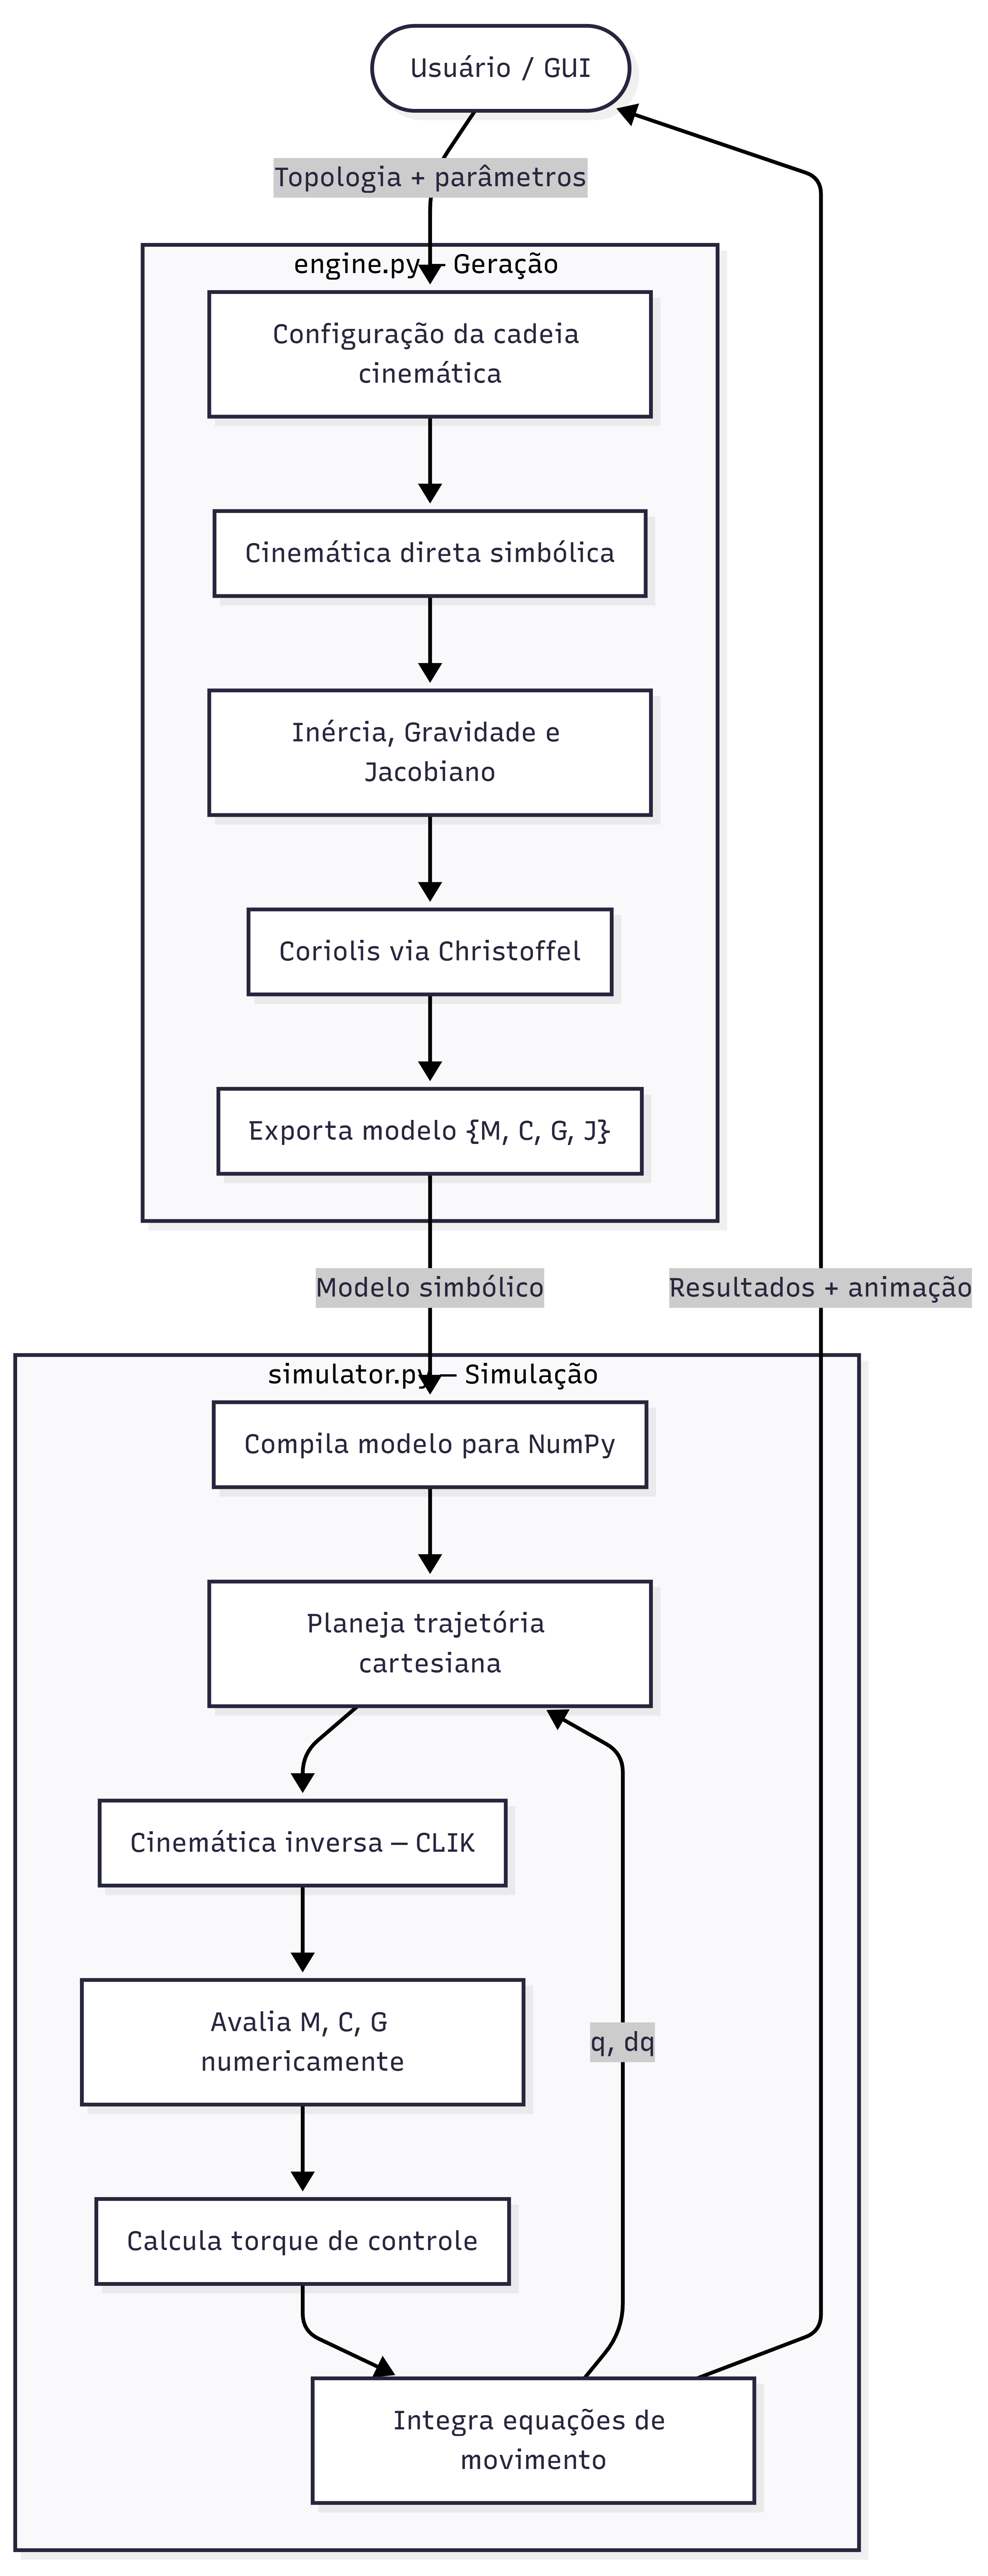
\includegraphics[width=0.50\textwidth]{figuras/Diagramas/Diagrama 1 — Arquitetura Geral do Sistema.png}
    \caption{Arquitetura geral do ambiente \textit{Hephaestus}: fluxo de trabalho desde a especificação da cadeia cinemática (módulo Modelagem) até a simulação em malha fechada (módulo Simulação) e a comparação de resultados (módulo Análise). As dependências entre os módulos \texttt{engine.py} e \texttt{simulator.py} e os quatro controladores não-lineares são destacadas.}
    \label{fig:arquitetura_geral}
\end{figure}

\section{Objetivos}

\subsection{Objetivo Geral}
Desenvolver um ambiente computacional integrado em Python para a modelagem dinâmica simbólica e simulação de manipuladores robóticos e sistemas UVMS. O projeto visa implementar uma arquitetura que automatize a derivação das equações de movimento via formulação Lagrangiana e execute simulações de controle em malha fechada com alto desempenho, considerando explicitamente os efeitos hidrodinâmicos, o controle no \emph{espaço de tarefa 6D} (posição $+$ orientação) e a comparação entre múltiplas estratégias de controle não-linear.

\paragraph{O que é o espaço de tarefa 6D.}
O termo ``6D'' refere-se à descrição completa da \emph{pose} do efetuador no espaço cartesiano, dada por seis coordenadas independentes: três para a \textbf{posição} e três para a \textbf{orientação}. As três coordenadas de posição $(x, y, z)$ localizam um ponto de referência do efetuador no espaço, enquanto as três coordenadas de orientação , tipicamente representadas por ângulos de \textit{roll}, \textit{pitch} e \textit{yaw} ou, equivalentemente, pelo eixo-ângulo de uma rotação em $SO(3)$ , descrevem a sua atitude angular. Tarefas de robótica que envolvem alinhar uma ferramenta a uma superfície, soldar ao longo de uma trajetória ou inserir uma peça em um furo exigem o controle simultâneo dessas seis coordenadas, e não apenas das três posicionais. Por essa razão, o \textit{Hephaestus} estende o algoritmo de cinemática inversa em malha fechada (CLIK) para operar com o Jacobiano completo $J \in \mathbb{R}^{6 \times N}$ , Capítulo~\ref{cap:revisao} , que mapeia as $N$ velocidades de junta para as seis componentes da \textit{twist} cartesiana (três lineares + três angulares).

\subsection{Objetivos Específicos}
\label{sec:Objetivos}

A fim de atingir o objetivo geral, foram definidos os seguintes objetivos específicos:

\begin{itemize}
    \item \textbf{Revisão Bibliográfica e Metodológica:} Analisar as abordagens clássicas de modelagem (Craig, Spong) e as especificidades da hidrodinâmica de UVMS (Fossen, Antonelli), identificando as limitações das ferramentas de simulação atuais.

    \item \textbf{Desenvolvimento da \textit{Engine} Matemática:} Implementar algoritmos em Python capazes de gerar simbolicamente as matrizes de Inércia ($M$), o vetor de Coriolis e Centrípeto ($C$) e o vetor de Gravidade/Empuxo ($G$) para manipuladores genéricos de $N$ graus de liberdade, tanto em ambiente terrestre quanto subaquático. No cenário subaquático, a massa adicionada é modelada como um tensor diagonal $6 \times 6$ por elo (três componentes translacionais e três rotacionais), rotacionado para o referencial global, em conformidade com a formulação de Fossen \cite{fossen2011handbook}.

    \item \textbf{Otimização Computacional:} Desenvolver um método de compilação das equações simbólicas para funções numéricas otimizadas por meio do \texttt{lambdify} com Eliminação de Subexpressões Comuns (CSE), superando os gargalos de desempenho típicos de simulações simbólicas puras. Implementar dois níveis de paralelismo: (i) na \textit{fase de derivação} do modelo, paralelizando o cálculo de $\partial M/\partial q_k$ e das linhas do vetor $C$ entre múltiplos processos; e (ii) na \textit{fase de simulação}, por meio de um executor de processos persistente (\texttt{ProcessPoolExecutor}) que avalia $M$, $C$ e $G$ numericamente em paralelo a cada passo de integração, eliminando o custo de \textit{respawn} entre execuções.

    \item \textbf{Implementação do Simulador Numérico:} Construir um ambiente de simulação capaz de resolver a dinâmica direta e inversa, incluindo: planejamento de trajetórias (segmentos de reta e arcos circulares com polinômio cúbico de interpolação); modelos de atrito nas juntas (Coulomb + viscoso, suavizados por $\tanh$ para evitar descontinuidades); e modelos de arrasto hidrodinâmico no espaço de juntas (linear e quadrático). Incluir visualização gráfica animada dos resultados.

    \item \textbf{Controle de Orientação no Espaço de Tarefa 6D:} Estender o algoritmo de Cinemática Inversa em Malha Fechada (CLIK) para o espaço de tarefa completo de seis dimensões, em que as três primeiras correspondem à posição cartesiana $(x, y, z)$ do efetuador e as três últimas à sua orientação angular (\textit{roll}, \textit{pitch}, \textit{yaw}), utilizando o Jacobiano completo $J \in \mathbb{R}^{6 \times N}$. Implementar múltiplos modos de referência de orientação: \textit{Livre}, \textit{Fixa}, \textit{Tangente à Trajetória}, \textit{Apontar para o Alvo}, interpolação SLERP (\textit{Spherical Linear Interpolation}) \cite{shoemake1985animating} e \textit{Normal à Superfície}.

    \item \textbf{Projeto e Validação de Controle:} Implementar e comparar quatro estratégias de controle não-linear em malha fechada:
    \begin{enumerate}
        \item \textbf{Controle por Torque Computado com PID} (CTC-PID): linearização por realimentação com termo integral \cite{craig1989introduction}, acrescido de uma compensação \textit{anti-windup} para evitar a instabilidade frente à saturação dos atuadores \cite{ogata2010modern}
        \item \textbf{Controle por Modo Deslizante} (CT-SMC): superfície deslizante \cite{slotine1991applied} com camada limite suavizante ($\tanh$) \cite{burton1986continuous};
        \item \textbf{Super-Twisting SMC} (STA): algoritmo de modo deslizante de 2ª ordem com sinal de controle contínuo e convergência em tempo finito \cite{levant1993sliding, moreno2012strict};
        \item \textbf{Controle por Rejeição Ativa de Distúrbios} (LADRC): observador de estado estendido (ESO) descentralizado com estimação e cancelamento em malha fechada dos distúrbios residuais \cite{han2009pid}.
    \end{enumerate}
    Todos os controladores são alimentados pelo algoritmo de Cinemática Inversa em Malha Fechada (CLIK). O tratamento de singularidades é realizado pelo método de Mínimos Quadrados Amortecidos (DLS) , formulado originalmente como Inversa Robusta a Singularidades (SR-Inverse) \cite{nakamura1986inverse} ,, e a gestão de redundância é estruturada via projeção no Espaço Nulo \cite{chiaverini1997singularity}.
\end{itemize}

\section{Metodologia}

A metodologia adotada estrutura-se em uma abordagem incremental de desenvolvimento de software e validação matemática:

\subsection{Modelagem Matemática (A Camada \textit{Engine})} Utilizando a biblioteca SymPy , em particular o módulo \texttt{dynamicsymbols} da mecânica analítica, que fornece símbolos dependentes do tempo com diferenciação automática , será implementada a formulação de Euler-Lagrange. Diferente de abordagens numéricas de caixa-preta, o software deduzirá as equações literais. Para o cenário subaquático, serão incorporados os termos de energia potencial aparente (Peso - Empuxo) e energia cinética modificada (Massa Adicionada como tensor 6D por elo), conforme Fossen \cite{fossen2011handbook}. O vetor resultante $C(q, \dot{q})$ unifica os efeitos de Coriolis e centrípeto pela formulação dos símbolos de Christoffel de primeira espécie \cite{spong2020robot}.

\subsection{Transição Simbólico-Numérica e Otimização}
Esta etapa foca na eficiência computacional e na superação do gargalo de desempenho típico de álgebras simbólicas. As equações dinâmicas geradas serão compiladas via \texttt{lambdify} com CSE (\textit{Common Subexpression Elimination}) ativo, que identifica e fatoriza subexpressões repetidas na expressão simbólica antes da geração do código NumPy, reduzindo o tamanho do \textit{bytecode} compilado e acelerando a avaliação numérica \cite{meurer2017sympy}.

Para lidar com a complexidade computacional do termo de Coriolis em sistemas de múltiplos graus de liberdade, será implementado processamento paralelo em dois níveis distintos. No primeiro nível, a derivação simbólica de $\partial M/\partial q_k$ e o cálculo das linhas do vetor $C$ são distribuídos entre múltiplos processos via \texttt{ProcessPoolExecutor}, visando otimizar o tempo de geração do modelo conforme as métricas de eficiência discutidas por Hollerbach \cite{hollerbach1980recursive}. No segundo nível, durante a simulação, um executor de processos persistente , pré-inicializado após a compilação e reutilizado em todos os ciclos subsequentes , avalia $M(q)$, $C(q, \dot{q})$ e $G(q)$ em paralelo a cada passo de integração, eliminando o custo de instanciação repetida de \textit{workers}.

\subsection{Simulação e Controle (A Camada \textit{Simulator}) }
\label{sec:simulador}
Será desenvolvido um integrador numérico Simplético de Euler operando em malha fechada. A escolha pelo método Simplético (atualização de $q$ antes de $\dot{q}$) em detrimento do Euler Explícito padrão é motivada pela melhor preservação da energia do sistema ao longo da trajetória. O passo de integração física pode ser subdividido (\textit{substeps}) de forma independente do passo de visualização, permitindo alta fidelidade numérica sem custo proporcional de renderização.

O controle dinâmico será realizado por uma das quatro estratégias implementadas (CTC-PID, CT-SMC, STA ou LADRC), todas alimentadas por um algoritmo de Cinemática Inversa em Malha Fechada (CLIK). A fase de inicialização da postura utiliza um algoritmo de Levenberg-Marquardt com busca em linha adaptativa, que ajusta dinamicamente o parâmetro de amortecimento $\lambda$ para garantir convergência robusta antes do início da trajetória. Durante a simulação, o CLIK opera no espaço de tarefa 6D (posição + orientação), incorporando: referência de velocidade e aceleração por \textit{feedforward}, correção de deriva do Jacobiano ($\dot{J}\dot{q}$), tratamento de singularidades via DLS \cite{nakamura1986inverse} e gestão de redundância via projeção no Espaço Nulo \cite{chiaverini1997singularity}.

Modelos de atrito nas juntas (Coulomb + viscoso, suavizados por $\tanh$) e de arrasto hidrodinâmico no espaço de juntas (linear e quadrático) são aplicados na equação de integração como forças passivas, separadamente do sinal de controle.

\subsection{Validação Comparativa}
O software desenvolvido (\textit{Hephaestus}) será submetido a testes de trajetória em dois cenários distintos: um manipulador serial em ambiente terrestre e um UVMS em ambiente submerso. A validação do cenário submerso seguirá os critérios de modelagem hidrodinâmica estabelecidos por Fossen e Antonelli \cite{fossen2011handbook, antonelli2014modelling}, analisando comparativamente os torques requeridos, o erro de rastreamento de posição e orientação, e o comportamento frente a perturbações externas para confirmar a consistência física dos termos de massa adicionada e empuxo implementados. A comparação entre as quatro estratégias de controle será realizada na aba de \textbf{Análise} da interface gráfica, que permite sobrepor múltiplas sessões de simulação nos mesmos gráficos.

  \chapter{Revisão Bibliográfica e Fundamentos Teóricos}
\label{cap:revisao}

Este capítulo apresenta a fundamentação teórica e a revisão da literatura sobre os tópicos centrais que sustentam o desenvolvimento do ambiente \textit{Hephaestus}. As áreas abordadas compreendem a modelagem cinemática e dinâmica de manipuladores robóticos, os fundamentos específicos dos Sistemas Manipuladores-Veículos Subaquáticos (UVMS), os algoritmos de cinemática inversa numérica, as estratégias de controle não-linear implementadas e os paradigmas de computação simbólica e numérica explorados. A revisão prioriza referências seminais e trabalhos recentes que fundamentam diretamente as escolhas de projeto e implementação.

% ==============================================================================
\section{Robótica de Manipuladores: Cinemática e Dinâmica}
% ==============================================================================

\subsection{Cinemática de Corpos Rígidos}

O estudo sistemático da posição e orientação de corpos rígidos no espaço constitui a base da robótica de manipuladores. A representação por matrizes de transformação homogênea $4 \times 4$, que codificam simultaneamente rotação e translação, foi popularizada por Denavit e Hartenberg \cite{denavit1955kinematic}, cuja convenção parametriza o posicionamento de elos sequenciais por apenas quatro parâmetros por junta: $a_i$, $d_i$, $\alpha_i$ e $\theta_i$. Embora a convenção DH permaneça amplamente utilizada no ensino, a representação por matrizes de rotação diretas (eixo-ângulo) adotada neste trabalho oferece maior transparência algébrica e facilita a integração com ferramentas de computação simbólica \cite{craig1989introduction, spong2020robot}.

A cinemática direta (FK) mapeia as variáveis de junta $q \in \mathbb{R}^N$ para a posição e orientação do efetuador final no espaço cartesiano. Para uma cadeia serial aberta de $N$ graus de liberdade, a transformação homogênea acumulada $T_N$ é obtida pelo produto:
\begin{equation}
    T_N(q) = T_1(q_1) \cdot T_2(q_2) \cdots T_N(q_N),
\end{equation}
onde:
\begin{itemize}
    \item $T_N(q) \in \mathbb{R}^{4\times 4}$ é a transformação homogênea acumulada do referencial da base até o efetuador final;
    \item $T_i(q_i) \in \mathbb{R}^{4\times 4}$ é a transformação homogênea associada à junta $i$ e ao elo $i$;
    \item $q_i$ é a variável generalizada (ângulo ou deslocamento) da junta $i$;
    \item $N$ é o número de graus de liberdade da cadeia \cite{spong2020robot}.
\end{itemize}

A cinemática diferencial relaciona as velocidades no espaço de juntas às velocidades no espaço cartesiano por meio do Jacobiano geométrico $J(q) \in \mathbb{R}^{6 \times N}$:
\begin{equation}
    \dot{x} = J(q)\dot{q},
    \label{eq:jacobian}
\end{equation}
onde:
\begin{itemize}
    \item $\dot{x} = [\dot{p}^\top,\, \omega^\top]^\top \in \mathbb{R}^{6}$ é o vetor de \textit{twist} do efetuador, reunindo a velocidade linear $\dot{p} \in \mathbb{R}^{3}$ e a velocidade angular $\omega \in \mathbb{R}^{3}$;
    \item $J(q) \in \mathbb{R}^{6\times N}$ é o Jacobiano geométrico, decomposto em linhas translacionais $J_v$ e linhas rotacionais $J_\omega$;
    \item $\dot{q} \in \mathbb{R}^{N}$ é o vetor de velocidades das juntas;
    \item $N$ é o número de graus de liberdade da cadeia.
\end{itemize}
A decomposição de $J$ em $J_v$ e $J_\omega$ é fundamental para o projeto dos controladores em espaço de tarefa \cite{siciliano2009robotics}: as três primeiras linhas, $J_v \in \mathbb{R}^{3 \times N}$, mapeiam $\dot{q}$ na velocidade linear $\dot{p}$, enquanto as três últimas, $J_\omega \in \mathbb{R}^{3 \times N}$, mapeiam $\dot{q}$ na velocidade angular $\omega$. Essa estrutura é o que define o chamado \emph{espaço de tarefa 6D}, em que três coordenadas descrevem a \textbf{posição} cartesiana e três descrevem a \textbf{orientação} angular do efetuador, totalizando seis graus de liberdade do efetuador no espaço.

As singularidades cinemáticas , configurações em que $J$ perde posto , representam pontos de degeneração do mapeamento diferencial, causando velocidades de junta ilimitadas para movimentos cartesianos finitos. Sua análise e tratamento, seja por critério do determinante de $JJ^\top$, por decomposição em valores singulares (SVD) \cite{golub2013matrix} ou por regularização do tipo Mínimos Quadrados Amortecidos (DLS), é abordada em detalhe por Nakamura e Hanafusa \cite{nakamura1986inverse} e Wampler \cite{wampler2007manipulator}.

\subsection{Dinâmica de Manipuladores: Formulação de Euler-Lagrange}

A modelagem dinâmica de manipuladores pode ser abordada por dois formalismos clássicos: Newton-Euler e Euler-Lagrange. A formulação de Newton-Euler é recursiva e numericamente eficiente , sua versão recursiva, proposta por Luh, Walker e Paul, tem complexidade $O(N)$ no número de elos \cite{luh1980online}. Já a formulação de Euler-Lagrange, adotada neste trabalho, deriva equações explícitas e simbólicas, tornando-a especialmente adequada para plataformas didáticas e para a síntese de controladores baseados em modelo.

O Lagrangiano $\mathcal{L} = T - V$, diferença entre a energia cinética $T$ e a potencial $V$ do sistema, conduz às equações de movimento de Euler-Lagrange:
\begin{equation}
    \frac{d}{dt}\left(\frac{\partial \mathcal{L}}{\partial \dot{q}_i}\right) - \frac{\partial \mathcal{L}}{\partial q_i} = \tau_i, \quad i = 1, \ldots, N.
    \label{eq:euler_lagrange}
\end{equation}
onde:
\begin{itemize}
    \item $\mathcal{L}(q,\dot{q}) = T - V$ é o Lagrangiano do sistema;
    \item $T(q,\dot{q})$ é a energia cinética total;
    \item $V(q)$ é a energia potencial total;
    \item $q_i$ e $\dot{q}_i$ são a coordenada e a velocidade generalizadas da junta $i$;
    \item $\tau_i$ é o torque generalizado aplicado na junta $i$;
    \item $N$ é o número de graus de liberdade.
\end{itemize}

O desenvolvimento da Equação \eqref{eq:euler_lagrange} para uma cadeia serial resulta na forma estruturada da equação de movimento:
\begin{equation}
    M(q)\ddot{q} + C(q,\dot{q})\dot{q} + G(q) = \tau,
    \label{eq:motion_equation}
\end{equation}
onde:
\begin{itemize}
    \item $M(q) \in \mathbb{R}^{N \times N}$ é a matriz de inércia generalizada, simétrica e definida positiva;
    \item $C(q,\dot{q}) \in \mathbb{R}^{N \times N}$ é a matriz de Coriolis e termos centrípetos;
    \item $G(q) \in \mathbb{R}^{N}$ é o vetor de gradiente de energia potencial gravitacional;
    \item $q, \dot{q}, \ddot{q} \in \mathbb{R}^{N}$ são, respectivamente, os vetores de posições, velocidades e acelerações generalizadas;
    \item $\tau \in \mathbb{R}^{N}$ é o vetor de torques generalizados aplicados pelos atuadores \cite{craig1989introduction, spong2020robot, siciliano2009robotics}.
\end{itemize}

Os elementos $C_{ij}$ da matriz de Coriolis são calculados pelos símbolos de Christoffel de segunda espécie \cite{spong2020robot}:
\begin{equation}
    C_{ij}(q,\dot{q}) = \sum_{k=1}^{N} c_{ijk}(q)\,\dot{q}_k, \quad
    c_{ijk} = \frac{1}{2}\left(\frac{\partial M_{ij}}{\partial q_k} + \frac{\partial M_{ik}}{\partial q_j} - \frac{\partial M_{jk}}{\partial q_i}\right).
    \label{eq:christoffel}
\end{equation}
onde:
\begin{itemize}
    \item $C_{ij}(q,\dot{q})$ é o elemento $(i,j)$ da matriz de Coriolis;
    \item $c_{ijk}(q)$ são os símbolos de Christoffel de segunda espécie;
    \item $M_{ij}, M_{ik}, M_{jk}$ são elementos da matriz de inércia $M(q)$;
    \item $\partial M_{ab}/\partial q_c$ denota a derivada parcial do elemento $M_{ab}$ em relação à coordenada $q_c$;
    \item $\dot{q}_k$ é a velocidade generalizada da junta $k$;
    \item $N$ é o número de graus de liberdade.
\end{itemize}

A matriz de inércia pode ser expressa em termos dos Jacobianos de velocidade linear $J_{v_i}$ e angular $J_{\omega_i}$ do centro de massa do elo $i$:
\begin{equation}
    M(q) = \sum_{i=1}^{N} \left[ m_i J_{v_i}^\top J_{v_i} + J_{\omega_i}^\top I_i^{(g)} J_{\omega_i} \right],
    \label{eq:inertia_matrix}
\end{equation}
onde:
\begin{itemize}
    \item $M(q) \in \mathbb{R}^{N\times N}$ é a matriz de inércia generalizada;
    \item $m_i$ é a massa do elo $i$;
    \item $J_{v_i} \in \mathbb{R}^{3\times N}$ e $J_{\omega_i} \in \mathbb{R}^{3\times N}$ são os Jacobianos linear e angular do CM do elo $i$;
    \item $I_i^{(g)} = R_i\, I_i^{(l)}\, R_i^\top \in \mathbb{R}^{3\times 3}$ é o tensor de inércia do elo $i$ expresso no referencial global, obtido pela transformação do tensor local $I_i^{(l)}$ pela matriz de rotação acumulada $R_i$ \cite{siciliano2009robotics};
    \item $N$ é o número de elos.
\end{itemize} Esta formulação, denominada \textit{método do Jacobiano da inércia}, é a base da implementação na classe \texttt{RobotMathEngine}.

A eficiência computacional do cálculo de $C(q,\dot{q})$ é crítica em sistemas com muitos graus de liberdade. Hollerbach \cite{hollerbach1980recursive} demonstrou que a formulação recursiva Newton-Euler reduz a complexidade de $O(N^4)$ (Lagrange ingênuo) para $O(N)$. Em abordagens simbólicas como a deste trabalho, a paralelização da computação de $\partial M/\partial q_k$ mitiga esse custo.

\subsection{Propriedades Estruturais da Dinâmica}

A estrutura da Equação \eqref{eq:motion_equation} exibe propriedades que são centrais para a análise de estabilidade e o projeto de controladores \cite{slotine1991applied, spong2020robot}:

\begin{enumerate}
    \item \textbf{Simetria e positividade de $M(q)$:} $M(q) = M(q)^\top > 0$ para todo $q$.
    \item \textbf{Antissimetria de $\dot{M} - 2C$:} A matriz $N(q,\dot{q}) = \dot{M}(q) - 2C(q,\dot{q})$ é antissimétrica, i.e., $x^\top N x = 0$ para todo $x$. Esta propriedade é a base da prova de estabilidade de Lyapunov para o controle por torque computado.
    \item \textbf{Linearidade nos parâmetros:} A equação de movimento pode ser reescrita como $M\ddot{q} + C\dot{q} + G = Y(q,\dot{q},\ddot{q})\,\theta$, onde $Y$ é a \textit{matriz de regressores} e $\theta$ é o vetor de parâmetros inerciais. Isso sustenta os controladores adaptativos \cite{slotine1987adaptive}.
\end{enumerate}

% ==============================================================================
\section{Sistemas Manipuladores-Veículos Subaquáticos (UVMS)}
% ==============================================================================

\subsection{Contexto e Motivação}

Os robôs subaquáticos representam uma das fronteiras mais ativas da engenharia mecatrônica e oceânica. Desde os primeiros estudos sistemáticos de Yuh \cite{yuh1990modeling}, a modelagem de Veículos Subaquáticos Não Tripulados (UUVs) evoluiu para incorporar a análise de sistemas acoplados veículo-manipulador, os UVMSs. A revisão abrangente de Yuh e West \cite{yuh2001underwater} cataloga as aplicações práticas , inspeção de dutos, manutenção de plataformas \textit{offshore}, arqueologia submarina e pesquisa oceanográfica , que motivam a crescente demanda por autonomia e precisão.

Trabalhos mais recentes, como a revisão de Sivčev et al. \cite{sivcev2018underwater}, confirmam que a principal barreira para a automação plena de UVMSs reside na complexidade da interação dinâmica veículo-braço e nas incertezas do meio aquático. Aldhaheri et al. \cite{aldhaheri2022underwater} fornecem uma revisão atualizada dos avanços em controle e navegação, reforçando a necessidade de simuladores de alta fidelidade para o desenvolvimento e validação de estratégias de controle antes do ensaio físico.

\subsection{Hidrodinâmica: Fundamentos e Formulação}

A modelagem hidrodinâmica de corpos submersos tem como referência fundamental o livro de Thor I. Fossen, \textit{Handbook of Marine Craft Hydrodynamics and Motion Control} \cite{fossen2011handbook}. Fossen sistematiza a modelagem baseada na formulação SNAME, onde as forças e momentos hidrodinâmicos atuantes sobre um corpo rígido submerso são decompostos em três categorias principais:

\paragraph{Massa Adicionada (\textit{Added Mass}).}
Ao acelerar um corpo submerso, é necessário acelerar também o fluido ao seu redor. Esse efeito é modelado como uma inércia adicional , a massa adicionada , capturada pelo tensor $M_A \in \mathbb{R}^{6 \times 6}$ \cite{fossen2011handbook, newman1977marine}:
\begin{equation}
    M_A = -\frac{\partial}{\partial \dot{\nu}}\left[\text{forças e momentos hidrodinâmicos}\right],
    \label{eq:added_mass_def}
\end{equation}
onde:
\begin{itemize}
    \item $M_A \in \mathbb{R}^{6\times 6}$ é o tensor de massa adicionada do corpo submerso;
    \item $\nu = [u,\, v,\, w,\, p,\, q,\, r]^\top \in \mathbb{R}^{6}$ é o vetor de velocidades no referencial do corpo (\textit{body-fixed}), com $u, v, w$ velocidades lineares (\textit{surge}, \textit{sway}, \textit{heave}) e $p, q, r$ velocidades angulares (\textit{roll}, \textit{pitch}, \textit{yaw});
    \item $\dot{\nu}$ é a derivada temporal de $\nu$ (acelerações lineares e angulares);
    \item o sinal negativo segue a convenção de Fossen, em que $M_A$ representa a inércia virtual sentida pelo corpo devido ao fluido acelerado.
\end{itemize}
Para corpos com planos de simetria, $M_A$ torna-se diagonal ou quase-diagonal \cite{fossen2011handbook}. No \textit{Hephaestus}, $M_A$ é modelado como um tensor diagonal $6 \times 6$ por elo, com três componentes translacionais $(m_{a,u}, m_{a,v}, m_{a,w})$ e três rotacionais $(m_{a,p}, m_{a,q}, m_{a,r})$, rotacionado para o referencial global conforme a formulação de Fossen \cite{fossen2011handbook}:
\begin{equation}
    M_{A}^{(g)} = R_i\,M_{A,\text{lin}}^{(l)}\,R_i^\top, \quad
    I_{A}^{(g)} = R_i\,M_{A,\text{rot}}^{(l)}\,R_i^\top.
\end{equation}
onde:
\begin{itemize}
    \item $M_{A}^{(g)} \in \mathbb{R}^{3\times 3}$ é a matriz de massa adicionada translacional do elo $i$ no referencial global;
    \item $I_{A}^{(g)} \in \mathbb{R}^{3\times 3}$ é a matriz de massa adicionada rotacional do elo $i$ no referencial global;
    \item $M_{A,\text{lin}}^{(l)}, M_{A,\text{rot}}^{(l)} \in \mathbb{R}^{3\times 3}$ são as matrizes diagonais de massa adicionada translacional e rotacional no referencial local;
    \item $R_i \in \mathbb{R}^{3\times 3}$ é a matriz de rotação acumulada até o elo $i$.
\end{itemize}

A contribuição da massa adicionada à matriz de inércia generalizada do UVMS é, portanto:
\begin{equation}
    M_{\text{Hydro}}(q) = \sum_{i=1}^{N} \left[ J_{v_i}^\top (m_i I + M_{A,i}^{(g)}) J_{v_i} + J_{\omega_i}^\top (I_i^{(g)} + I_{A,i}^{(g)}) J_{\omega_i} \right].
    \label{eq:M_hydro}
\end{equation}
onde:
\begin{itemize}
    \item $M_{\text{Hydro}}(q) \in \mathbb{R}^{N\times N}$ é a matriz de inércia generalizada do UVMS;
    \item $m_i I$ é a inércia rígida translacional do elo $i$, com $I = I_3$ (identidade $3\times 3$);
    \item $M_{A,i}^{(g)} \in \mathbb{R}^{3\times 3}$ é a massa adicionada translacional do elo $i$ no referencial global;
    \item $I_i^{(g)} \in \mathbb{R}^{3\times 3}$ é o tensor de inércia rígida do elo $i$ no referencial global;
    \item $I_{A,i}^{(g)} \in \mathbb{R}^{3\times 3}$ é a massa adicionada rotacional do elo $i$ no referencial global;
    \item $J_{v_i}, J_{\omega_i} \in \mathbb{R}^{3\times N}$ são os Jacobianos linear e angular do elo $i$.
\end{itemize}
Esta formulação, diretamente implementada no método \texttt{step\_2\_jacobian\_M\_G} da classe \texttt{RobotMathHydro}, garante que a contribuição de inércia aparente seja corretamente projetada no espaço de juntas via Jacobianos \cite{antonelli2014modelling}.

\paragraph{Arrasto Hidrodinâmico (\textit{Drag}).}
O arrasto sobre um corpo submerso em movimento possui componentes viscosa (linear em $\nu$) e de pressão (quadrática em $\nu$). A formulação simplificada, mas amplamente adotada em simuladores de UVMS \cite{antonelli2014modelling, fossen2011handbook}, escreve o vetor de forças de arrasto no espaço de juntas como:
\begin{equation}
    \tau_{\text{drag}} = D_{\text{lin}}\,\dot{q} + D_{\text{quad}}\,|\dot{q}|\,\dot{q},
    \label{eq:drag}
\end{equation}
onde:
\begin{itemize}
    \item $\tau_{\text{drag}} \in \mathbb{R}^{N}$ é o vetor de torques de arrasto no espaço de juntas;
    \item $D_{\text{lin}} \in \mathbb{R}^{N}$ é o vetor de coeficientes de arrasto linear (regime laminar);
    \item $D_{\text{quad}} \in \mathbb{R}^{N}$ é o vetor de coeficientes de arrasto quadrático (regime turbulento);
    \item $\dot{q} \in \mathbb{R}^{N}$ é o vetor de velocidades das juntas;
    \item $|\dot{q}|$ denota o vetor componente a componente do valor absoluto de $\dot{q}$;
    \item os produtos $D_{\text{lin}}\,\dot{q}$ e $D_{\text{quad}}\,|\dot{q}|\,\dot{q}$ são realizados elemento por elemento.
\end{itemize}
Essa formulação é modelada como força passiva no integrador Simplético, conforme discutido na Seção \ref{sec:simulador}.

\paragraph{Força de Empuxo e Gradiente Estático (\textit{Buoyancy}).}
O princípio de Arquimedes estabelece que um corpo submerso experimenta uma força de empuxo $B = \rho g V_{\text{sub}}$, onde $\rho$ é a densidade do fluido, $g$ é a aceleração gravitacional e $V_{\text{sub}}$ é o volume deslocado \cite{newman1977marine}. Para um elo submerso, o potencial aparente é:
\begin{equation}
    V_i^{\text{app}} = (m_i - \rho\,\text{vol}_i)\,g\,z_{\text{cm},i},
    \label{eq:buoyancy_potential}
\end{equation}
onde:
\begin{itemize}
    \item $V_i^{\text{app}}$ é a energia potencial aparente (peso menos empuxo) do elo $i$;
    \item $m_i$ é a massa do elo $i$;
    \item $\rho\,\text{vol}_i$ é a massa de fluido deslocada pelo elo (princípio de Arquimedes);
    \item $\rho$ é a densidade do fluido, $\text{vol}_i$ é o volume submerso do elo;
    \item $g$ é a aceleração da gravidade;
    \item $z_{\text{cm},i}$ é a coordenada vertical do centro de massa do elo $i$.
\end{itemize} O vetor $G(q)$ resultante combina, portanto, o gradiente de Peso menos Empuxo, podendo ser nulo ou muito pequeno quando o elo é neutralmente flutuante ($m_i \approx \rho\,\text{vol}_i$), o que reduz os torques estáticos necessários e é o cenário típico de UVMSs projetados para neutralidade \cite{fossen2011handbook, antonelli2014modelling}.

\subsection{Modelo Dinâmico Completo do UVMS}

Antonelli \cite{antonelli2014modelling} apresenta o modelo dinâmico unificado de um UVMS como:
\begin{equation}
    M_{\text{Hydro}}(q)\ddot{q} + C_{\text{Hydro}}(q,\dot{q})\dot{q} + D(q,\dot{q})\dot{q} + G_{\text{Hydro}}(q) = \tau + J^\top f_{\text{ext}},
    \label{eq:uvms_model}
\end{equation}
onde:
\begin{itemize}
    \item $M_{\text{Hydro}}(q) \in \mathbb{R}^{N\times N}$ é a matriz de inércia generalizada com massa adicionada;
    \item $C_{\text{Hydro}}(q,\dot{q}) \in \mathbb{R}^{N\times N}$ é a matriz de Coriolis e termos centrípetos hidrodinâmica;
    \item $D(q,\dot{q}) \in \mathbb{R}^{N\times N}$ reúne os efeitos de arrasto linear e quadrático;
    \item $G_{\text{Hydro}}(q) \in \mathbb{R}^{N}$ é o vetor de torques aparentes (peso menos empuxo);
    \item $q, \dot{q}, \ddot{q} \in \mathbb{R}^{N}$ são posições, velocidades e acelerações generalizadas;
    \item $\tau \in \mathbb{R}^{N}$ é o vetor de torques aplicados pelos atuadores;
    \item $f_{\text{ext}} \in \mathbb{R}^{6}$ são as forças e momentos externos aplicados ao efetuador (e.g., interação com o ambiente);
    \item $J^\top \in \mathbb{R}^{N\times 6}$ é a transposta do Jacobiano geométrico, que projeta as forças cartesianas no espaço de juntas.
\end{itemize}
Esta estrutura é idêntica à da Equação \eqref{eq:motion_equation}, com os termos $M$, $C$ e $G$ modificados pela contribuição hidrodinâmica , o que permite que a mesma \textit{engine} seja reutilizada em ambos os modos (ar e água) com a simples extensão implementada em \texttt{RobotMathHydro}.

% ==============================================================================
\section{Cinemática Inversa Numérica}
% ==============================================================================

\subsection{Formulação do Problema}

A cinemática inversa (IK) , determinação das variáveis de junta $q$ que posicionam o efetuador em uma configuração cartesiana desejada $x_d$ , é um problema central em robótica. Para cadeias seriais não-redundantes ($N = 6$), soluções analíticas fechadas são, em geral, possíveis \cite{craig1989introduction}. Para sistemas redundantes ($N > 6$) ou com geometrias genéricas, as abordagens numéricas iterativas são necessárias \cite{siciliano2009robotics}.

\subsection{Cinemática Inversa em Malha Fechada (CLIK)}

O algoritmo de Cinemática Inversa em Malha Fechada (\textit{Closed-Loop Inverse Kinematics}, CLIK), proposto por Samson et al. \cite{samson1991robot} e refinado por Chiaverini et al. \cite{chiaverini1994review}, integra numericamente a equação diferencial de erro cartesiano para produzir uma referência de velocidade de junta que converge para a configuração desejada. A lei de atualização, na forma discreta com passo $dt$, é:
\begin{equation}
    \dot{q}_{k+1} = J^{\dagger}(q_k)\left[\dot{x}_d + K_P e_k\right] + \left(I - J^{\dagger}J\right)\dot{q}_0,
    \label{eq:clik}
\end{equation}
onde:
\begin{itemize}
    \item $\dot{q}_{k+1} \in \mathbb{R}^{N}$ é o vetor de velocidades de junta no próximo instante discreto;
    \item $J^{\dagger}(q_k) \in \mathbb{R}^{N\times m}$ é a pseudo-inversa (ou pseudo-inversa amortecida) do Jacobiano avaliado em $q_k$, com $m \in \{3, 6\}$ a dimensão da tarefa;
    \item $\dot{x}_d \in \mathbb{R}^{m}$ é a velocidade cartesiana de referência (\textit{feedforward});
    \item $e_k = x_d - x_k$ é o erro cartesiano (posição/orientação) no instante $k$;
    \item $K_P$ é o ganho proporcional de realimentação;
    \item $(I - J^{\dagger}J) \in \mathbb{R}^{N\times N}$ é o operador de projeção no espaço nulo de $J$;
    \item $\dot{q}_0 \in \mathbb{R}^{N}$ é a velocidade auxiliar usada para objetivos secundários (e.g., afastar-se de limites de junta) sem afetar a tarefa primária \cite{chiaverini1997singularity}.
\end{itemize}

O CLIK implementado no \textit{Hephaestus} opera no espaço de tarefa completo de seis dimensões (3 da posição e 3 da orientação angular do efetuador, totalizando \emph{seis graus de liberdade da tarefa}), utilizando o Jacobiano completo $J \in \mathbb{R}^{6 \times N}$ , que relaciona, conforme a Equação~\eqref{eq:jacobian}, as $N$ velocidades de junta com as três velocidades lineares e três velocidades angulares do efetuador , e incorpora:
\begin{itemize}
    \item \textbf{Feedforward de velocidade e aceleração:} contribuição de $\dot{x}_d$ e $\ddot{x}_d$ para melhorar o rastreamento;
    \item \textbf{Correção de deriva do Jacobiano:} subtração do termo $\dot{J}\dot{q}$ para compensar a aceleração já contabilizada na derivada temporal do Jacobiano \cite{siciliano2009robotics};
    \item \textbf{Gestão de redundância via Espaço Nulo:} projeção da lei de controle $K_n(q_{\text{home}} - q)$ no \textit{kernel} de $J$ para atrair o robô à postura preferida \cite{chiaverini1997singularity, liegeois1977automatic}.
\end{itemize}

\subsection{Tratamento de Singularidades: Mínimos Quadrados Amortecidos (DLS)}

Próximo às singularidades, os valores singulares de $J$ se aproximam de zero, tornando a pseudo-inversa $J^+ = J^\top(JJ^\top)^{-1}$ numericamente instável. Nakamura e Hanafusa \cite{nakamura1986inverse} propuseram a pseudo-inversa amortecida (DLS , \textit{Damped Least Squares}):
\begin{equation}
    J^{\dagger}_{\lambda} = J^\top\left(JJ^\top + \lambda^2 I\right)^{-1},
    \label{eq:dls}
\end{equation}
onde:
\begin{itemize}
    \item $J^{\dagger}_{\lambda} \in \mathbb{R}^{N\times m}$ é a pseudo-inversa amortecida (DLS) do Jacobiano;
    \item $J \in \mathbb{R}^{m\times N}$ é o Jacobiano (com $m \in \{3, 6\}$);
    \item $J^\top$ é a transposta do Jacobiano;
    \item $\lambda > 0$ é o fator de amortecimento, controla o compromisso entre precisão e estabilidade próximo de singularidades;
    \item $I \in \mathbb{R}^{m\times m}$ é a matriz identidade da mesma dimensão da tarefa.
\end{itemize} Wampler \cite{wampler2007manipulator} e Chiaverini et al. \cite{chiaverini1994review} analisaram as propriedades de estabilidade e a escolha ótima de $\lambda$ em função dos valores singulares mínimos de $J$. A abordagem de DLS com $\lambda$ variável (\textit{variable DLS}), descrita em Chiaverini et al. \cite{chiaverini1994review}, é especialmente robusta e consiste em aumentar $\lambda$ continuamente conforme o valor singular mínimo decresce.

\subsection{Inicialização por Levenberg-Marquardt com Busca em Linha}

Para a inicialização da postura antes do início da trajetória, o \textit{Hephaestus} utiliza uma variante do algoritmo de Levenberg-Marquardt \cite{marquardt1963algorithm, more2006levenberg}, que ajusta adaptativamente o parâmetro $\lambda$ entre iterações com base no sucesso da redução do erro, combinado com uma busca em linha por \textit{backtracking} (regra de Armijo \cite{armijo1966minimization}) para garantir descida suficiente a cada passo.

\subsection{Erros de Orientação e SLERP}

No espaço de tarefa 6D, as três últimas componentes correspondem à orientação angular do efetuador, codificada em $SO(3)$. Diferentemente da posição, em que o erro é simplesmente a diferença vetorial $e_p = P_d - P_c$, o erro de orientação não pode ser obtido pela subtração direta de matrizes de rotação, pois $SO(3)$ não é um espaço vetorial. Por isso, o erro de orientação é computado pela formulação de Anel \cite{chiaverini1997singularity}, via extração do vetor axial da parte antissimétrica do produto $R_d R_c^\top - R_c R_d^\top$:
\begin{equation}
    e_R = \frac{1}{2}\text{vee}\!\left(R_d R_c^\top - R_c R_d^\top\right),
    \label{eq:orient_error}
\end{equation}
onde:
\begin{itemize}
    \item $e_R \in \mathbb{R}^{3}$ é o vetor de erro de orientação (formulação axial);
    \item $R_d \in SO(3)$ é a matriz de rotação desejada do efetuador;
    \item $R_c \in SO(3)$ é a matriz de rotação corrente do efetuador;
    \item $\text{vee}(\cdot) : \mathfrak{so}(3) \to \mathbb{R}^{3}$ é o operador que extrai o vetor axial associado à parte antissimétrica de uma matriz $3\times 3$.
\end{itemize}
Esta formulação é proporcional ao eixo-ângulo para erros pequenos e evita singularidades de representação por ângulos de Euler \cite{siciliano2009robotics}.

Para a interpolação suave entre duas orientações, é utilizada a \textit{Spherical Linear Interpolation} (SLERP), proposta por Shoemake \cite{shoemake1985animating} no contexto de animação computacional. Dados dois quaternions (ou matrizes de rotação) $R_0$ e $R_f$, a SLERP define:
\begin{equation}
    R(s) = R_0 \left(R_0^\top R_f\right)^s, \quad s \in [0,1],
    \label{eq:slerp}
\end{equation}
onde:
\begin{itemize}
    \item $R(s) \in SO(3)$ é a matriz de rotação interpolada entre $R_0$ e $R_f$;
    \item $R_0 \in SO(3)$ é a rotação inicial;
    \item $R_f \in SO(3)$ é a rotação final desejada;
    \item $s \in [0, 1]$ é o parâmetro de interpolação (0 corresponde a $R_0$ e 1 a $R_f$);
    \item a operação $(\cdot)^s$ é a potência fracionária no grupo $SO(3)$, equivalente a $\exp(s \log(R_0^\top R_f))$;
    \item garante interpolação geodésica (caminho mais curto) sobre $SO(3)$ \cite{dam1998quaternions}.
\end{itemize}

% ==============================================================================
\section{Estratégias de Controle Não-Linear}
\label{sec:controle}
% ==============================================================================

\subsection{Controle por Torque Computado (CTC)}

O Controle por Torque Computado (\textit{Computed Torque Control}, CTC), derivado da linearização por realimentação (\textit{feedback linearization}) de Spong et al. \cite{spong2008robot}, é a estratégia fundamental de controle baseado em modelo para robôs. A lei de controle cancela a não-linearidade da dinâmica e impõe uma dinâmica linear de malha fechada:
\begin{equation}
    \tau = M(q)\left[\ddot{q}_d + K_D\dot{e} + K_P e + K_I \int e\, dt\right] + C(q,\dot{q})\dot{q} + G(q),
    \label{eq:ctc_pid}
\end{equation}
onde:
\begin{itemize}
    \item $\tau \in \mathbb{R}^{N}$ é o vetor de torque de controle aplicado;
    \item $M(q), C(q,\dot{q}), G(q)$ são as matrizes/vetor da dinâmica do robô (Equação~\eqref{eq:motion_equation});
    \item $\ddot{q}_d \in \mathbb{R}^{N}$ é a aceleração de referência (\textit{feedforward});
    \item $e = q_d - q \in \mathbb{R}^{N}$ é o erro de junta entre referência e estado corrente;
    \item $\dot{e}$ é a derivada temporal do erro;
    \item $K_P, K_D, K_I \in \mathbb{R}^{N\times N}$ são as matrizes de ganho proporcional, derivativo e integral, tipicamente diagonais.
\end{itemize}
Com modelo exato, a dinâmica de erro satisfaz $\ddot{e} + K_D\dot{e} + K_P e = 0$, que é um sistema linear de segunda ordem estável para $K_P, K_D > 0$ \cite{craig1989introduction}.

Na prática, erros de modelo introduzem distúrbios residuais. O termo integral (CTC-PID) melhora a rejeição a distúrbios constantes, mas requer \textit{anti-windup} para evitar saturação do integrador \cite{astrom1995theory}. A implementação no \textit{Hephaestus} inclui \textit{anti-windup} por clamping com limites ajustáveis.

\subsection{Controle por Modo Deslizante (SMC)}

O Controle por Modo Deslizante (\textit{Sliding Mode Control}, SMC) é uma técnica de controle robusto que garante convergência à superfície deslizante $S = \dot{e} + \lambda e = 0$ mesmo na presença de incertezas e perturbações limitadas. A referência canônica é o livro de Slotine e Li \cite{slotine1991applied}, que apresenta a análise de estabilidade via função de Lyapunov $V = \frac{1}{2}S^\top S$.

A lei de controle implementada no \textit{Hephaestus} segue a formulação por torque computado com superfície deslizante \cite{slotine1991applied}:
\begin{equation}
    \tau = M(q)\left[\ddot{q}_d - \lambda\dot{e} - K \tanh(S/\phi)\right] + C(q,\dot{q})\dot{q} + G(q),
    \label{eq:smc}
\end{equation}
onde:
\begin{itemize}
    \item $\tau \in \mathbb{R}^{N}$ é o vetor de torque de controle SMC;
    \item $M(q), C(q,\dot{q}), G(q)$ são os termos da dinâmica nominal do robô;
    \item $\ddot{q}_d$ é a aceleração de referência;
    \item $\dot{e}$ é a derivada do erro de junta;
    \item $\lambda$ é o parâmetro de pendente da superfície deslizante $S = \dot{e} + \lambda e$;
    \item $K$ é a matriz de ganhos de robustez (define a magnitude do torque de chaveamento);
    \item $\phi > 0$ é a espessura da camada limite que substitui a função $\text{sign}(S)$ pela $\tanh(S/\phi)$, eliminando o \textit{chattering} (oscilações de alta frequência) ao custo de uma robustez finita dentro da camada \cite{slotine1991applied, edwards1998sliding};
    \item $\tanh(\cdot)$ é aplicada componente a componente.
\end{itemize} A análise de robustez com camada limite foi formalizada por Burton e Zinober \cite{burton1986continuous}.

\subsection{Algoritmo Super-Twisting (STA)}

O algoritmo Super-Twisting (\textit{Super-Twisting Algorithm}, STA), proposto por Levant \cite{levant1993sliding}, é um modo deslizante de segunda ordem que elimina o \textit{chattering} intrinsecamente, produzindo um sinal de controle contínuo com convergência em tempo finito:
\begin{align}
    v_{\text{sw}} &= -k_1 |S|^{1/2} \text{sign}(S) + z, \label{eq:sta1}\\
    \dot{z} &= -k_2 \,\text{sign}(S), \label{eq:sta2}
\end{align}
onde:
\begin{itemize}
    \item $v_{\text{sw}}$ é o sinal de chaveamento contínuo do STA;
    \item $S$ é a variável de superfície deslizante (definida a partir do erro de junta);
    \item $|S|^{1/2}$ é a raiz quadrada do módulo de $S$, aplicada componente a componente;
    \item $\text{sign}(S)$ é a função sinal aplicada componente a componente;
    \item $k_1, k_2 > 0$ são os ganhos do STA, ajustados conforme a magnitude do distúrbio;
    \item $z$ é uma variável interna que integra o sinal descontínuo, produzindo $v_{\text{sw}}$ contínuo;
    \item $\dot{z}$ é a derivada temporal de $z$.
\end{itemize} Moreno e Osorio \cite{moreno2012strict} forneceram uma função de Lyapunov estrita para o STA, estabelecendo condições de ganho suficientes para rejeição de perturbações com derivada limitada: $k_2 > \delta$, $k_1 > 2\sqrt{k_2 \delta}$, onde $|\dot{d}| \leq \delta$. A convergência em tempo finito diferencia o STA do SMC de primeira ordem, cuja convergência é assintótica \cite{utkin2017sliding}.

\subsection{Controle por Rejeição Ativa de Distúrbios (ADRC/LADRC)}

O Controle por Rejeição Ativa de Distúrbios (\textit{Active Disturbance Rejection Control}, ADRC), proposto por Han \cite{han1995class} e popularizado em versão linear (LADRC) por Gao \cite{gao2003scaling}, é uma abordagem paradigmática de controle que interpreta todas as incertezas do modelo, dinâmicas não-modeladas e perturbações externas como um único ``distúrbio total'' $f(q,\dot{q},d,t)$, estimado em tempo real por um Observador de Estado Estendido (ESO) e cancelado pela lei de controle.

A dinâmica de segunda ordem de uma junta é reescrita como:
\begin{equation}
    \ddot{q}_i = b_0 \tau_i + f_i, \quad f_i \triangleq \text{distúrbio total},
    \label{eq:adrc_plant}
\end{equation}
onde:
\begin{itemize}
    \item $\ddot{q}_i$ é a aceleração da junta $i$;
    \item $\tau_i$ é o torque aplicado à junta $i$;
    \item $b_0$ é um ganho nominal conhecido (aqui, $b_0 \approx 1/M_{ii}$, sendo $M_{ii}$ o elemento diagonal da matriz de inércia);
    \item $f_i$ é o distúrbio total, que engloba acoplamentos dinâmicos com outras juntas, erros de modelo e perturbações externas.
\end{itemize}

O ESO de terceira ordem (linear) observa o estado aumentado $[q_i, \dot{q}_i, f_i]$:
\begin{align}
    \dot{z}_1 &= z_2 - \beta_1(z_1 - q_i), \label{eq:eso1}\\
    \dot{z}_2 &= z_3 - \beta_2(z_1 - q_i) + b_0\tau_i, \label{eq:eso2}\\
    \dot{z}_3 &= -\beta_3(z_1 - q_i), \label{eq:eso3}
\end{align}
onde:
\begin{itemize}
    \item $z_1, z_2, z_3$ são as estimativas de $q_i$, $\dot{q}_i$ e $f_i$ produzidas pelo ESO;
    \item $q_i$ é a posição medida da junta;
    \item $\tau_i$ é o torque aplicado;
    \item $b_0$ é o ganho nominal de canal;
    \item $\beta_1 = 3\omega_o$, $\beta_2 = 3\omega_o^2$, $\beta_3 = \omega_o^3$ são os ganhos do observador, parametrizados pela frequência de observador $\omega_o > 0$ \cite{gao2003scaling}.
\end{itemize}

A lei de controle cancela o distúrbio estimado $z_3$:
\begin{equation}
    \tau_i = \frac{u_0 - z_3}{b_0}, \quad u_0 = \ddot{q}_{d,i} + k_p(q_{d,i} - q_i) + k_d(\dot{q}_{d,i} - \dot{q}_i).
    \label{eq:adrc_control}
\end{equation}
onde:
\begin{itemize}
    \item $\tau_i$ é o torque de controle ADRC para a junta $i$;
    \item $u_0$ é o sinal de controle nominal (PD com \textit{feedforward} de aceleração);
    \item $z_3$ é a estimativa do distúrbio total $f_i$ produzida pelo ESO;
    \item $b_0$ é o ganho nominal de canal;
    \item $\ddot{q}_{d,i}, \dot{q}_{d,i}, q_{d,i}$ são as referências de aceleração, velocidade e posição da junta $i$;
    \item $k_p, k_d > 0$ são os ganhos proporcional e derivativo, respectivamente.
\end{itemize}

A análise de estabilidade do LADRC foi formalizada por Zheng e Gao \cite{zheng2010practical}. A formulação descentralizada , um ESO por junta, ignorando o acoplamento dinâmico , é especialmente atraente para robótica: Huang e Xue \cite{huang2014active} e trabalhos subsequentes demonstraram sua eficácia em manipuladores, onde os termos de Coriolis e gravidade são tratados como distúrbios a serem estimados pelo ESO. O artigo de revisão de Han \cite{han2009pid} sintetiza a motivação filosófica da abordagem ADRC como extensão natural do controlador PID.

No \textit{Hephaestus}, a implementação inclui feedforward explícito de $G(q)$ e $C(q,\dot{q})$, reduzindo o distúrbio residual que o ESO deve estimar para apenas erros de modelo e perturbações externas.

% ==============================================================================
\section{Planejamento de Trajetórias}
% ==============================================================================

O planejamento de trajetórias em robótica define os perfis de posição, velocidade e aceleração que o efetuador deve seguir ao longo do tempo. Siciliano et al. \cite{siciliano2009robotics} distinguem entre planejamento no espaço de juntas e no espaço cartesiano.

\subsection{Polinômio Cúbico e Perfil de \textit{Jerk} Finito}

Para interpolação de um ponto $P_i$ a um ponto $P_f$ em um tempo $T$, o polinômio cúbico (grau 3) garante continuidade de posição e velocidade nos extremos com velocidades inicial e final nulas \cite{siciliano2009robotics, craig1989introduction}:
\begin{equation}
    s(t) = 3\left(\frac{t}{T}\right)^2 - 2\left(\frac{t}{T}\right)^3,
    \label{eq:cubic_poly}
\end{equation}
onde:
\begin{itemize}
    \item $s(t) \in [0,1]$ é a variável de progresso normalizada da trajetória, com $s(0)=0$ e $s(T)=1$;
    \item $t$ é o tempo decorrido desde o início do trecho, com $0 \le t \le T$;
    \item $T$ é a duração total do trecho de trajetória.
\end{itemize}
A primeira derivada satisfaz $\dot{s}(0) = \dot{s}(T) = 0$ e a aceleração máxima é $\ddot{s}_{\max} = 6/T^2$ no instante $T/2$. O polinômio de grau 5, embora garanta continuidade de aceleração nos extremos (menor \textit{jerk}), não foi adotado aqui por apresentar valores de pico de aceleração ligeiramente superiores para o mesmo tempo de trajetória \cite{siciliano2009robotics}.

\subsection{Trajetória Circular no Espaço Cartesiano}

A trajetória circular é parametrizada por um centro $C$, dois vetores ortonormais $e_1$, $e_2$ no plano do arco, raio $R$ e ângulo total $\theta_f - \theta_0$:
\begin{equation}
    P(t) = C + R\left[\cos(\theta(t))\,e_1 + \sin(\theta(t))\,e_2\right],
    \label{eq:circle_traj_review}
\end{equation}
onde:
\begin{itemize}
    \item $P(t) \in \mathbb{R}^3$ é a posição cartesiana do efetuador em função do tempo;
    \item $C \in \mathbb{R}^3$ é o centro da circunferência;
    \item $R$ é o raio do arco;
    \item $e_1, e_2 \in \mathbb{R}^3$ são vetores unitários ortonormais que definem o plano do arco;
    \item $\theta(t) = \theta_0 + (\theta_f - \theta_0)\,s(t)$ é o ângulo varrido em função do tempo, sendo $\theta_0$ e $\theta_f$ os ângulos inicial e final do arco;
    \item $s(t)$ é o polinômio cúbico de Eq. \eqref{eq:cubic_poly}, que produz partida e chegada suaves.
\end{itemize}
As velocidade e aceleração cartesianas são obtidas pela diferenciação analítica de $P(t)$ \cite{siciliano2009robotics}.

% ==============================================================================
\section{Computação Simbólica e Geração de Código Numérico}
% ==============================================================================

\subsection{Álgebra Computacional Simbólica com SymPy}

O projeto SymPy \cite{meurer2017sympy} é uma biblioteca Python de Álgebra Computacional Simbólica (\textit{Computer Algebra System}, CAS) inteiramente implementada em Python puro, o que a torna portável e integrável sem dependências externas de compilação. Meurer et al. \cite{meurer2017sympy} descrevem a arquitetura modular do SymPy, destacando o módulo \texttt{sympy.physics.mechanics}, que fornece o tipo \texttt{dynamicsymbols} , símbolos dependentes do tempo com diferenciação automática , e as funções do método de Lagrange que automatizam a derivação das equações de movimento a partir da energia cinética e potencial.

A manipulação simbólica de expressões de grande porte , como as matrizes $M(q)$ de sistemas com 6 ou mais graus de liberdade , pode produzir expressões com dezenas de milhares de subexpressões primitivas. A gestão eficiente dessas expressões é crítica para viabilizar a simulação numérica subsequente \cite{leu1986automated}.

\subsection{Eliminação de Subexpressões Comuns (CSE)}

A Eliminação de Subexpressões Comuns (\textit{Common Subexpression Elimination}, CSE) é uma otimização clássica de compiladores \cite{alfred2007compilers} que identifica subexpressões repetidas em uma expressão aritmética e as substitui por variáveis temporárias, reduzindo o número total de operações elementares. No contexto da simulação robótica, Moses \cite{moses1971algebraic} demonstrou que a simplificação algébrica de expressões cinemáticas pode reduzir em mais de uma ordem de grandeza o número de operações necessárias.

A função \texttt{sp.lambdify()} do SymPy com a \textit{flag} \texttt{cse=True} aplica automaticamente a CSE antes de gerar o código Python/NumPy, detectando e fatorando subexpressões comuns nas matrizes $M$, $C$ e $G$ antes da geração do código numérico \cite{meurer2017sympy}. Isso reduz significativamente o tamanho do \textit{bytecode} compilado , crítico para evitar \texttt{MemoryError} em sistemas de grande porte , e acelera a avaliação numérica por reutilização de subexpressões em \textit{cache}.

\subsection{Paralelismo na Derivação Simbólica}

A derivação simbólica do vetor de Coriolis, que requer o cálculo de $\partial M / \partial q_k$ para $k = 1, \ldots, N$ e de todas as combinações de símbolos de Christoffel (Equação \eqref{eq:christoffel}), possui complexidade $O(N^3)$ em termos de operações simbólicas, tornando-se o principal gargalo de tempo para sistemas com muitos graus de liberdade.

O módulo \texttt{concurrent.futures.ProcessPoolExecutor} da biblioteca padrão do Python permite a distribuição dessas tarefas entre múltiplos processos, contornando o \textit{Global Interpreter Lock} (GIL) do CPython \cite{beazley2010understanding}. A abordagem de \textit{pool} de processos com passagem de dados simbólicos via \texttt{pickle} foi validada por Leu et al. \cite{leu1986automated} para sistemas de dinâmica multivariável de grande porte.

\subsection{Integração Numérica: Método de Euler Simplético}

A integração numérica das equações de movimento \eqref{eq:motion_equation} é realizada pelo método de Euler Simplético (também chamado de Euler Simplético de primeira ordem ou método de Euler semi-implícito). Em contraste com o Euler Explícito padrão (atualização de $q$ e $\dot{q}$ simultaneamente com valores do passo anterior), o Euler Simplético atualiza primeiro a velocidade e depois a posição:
\begin{align}
    \dot{q}^{n+1} &= \dot{q}^n + \ddot{q}^n \Delta t, \label{eq:symplectic_euler1}\\
    q^{n+1} &= q^n + \dot{q}^{n+1} \Delta t. \label{eq:symplectic_euler2}
\end{align}
onde:
\begin{itemize}
    \item $q^n, \dot{q}^n, \ddot{q}^n$ são, respectivamente, a posição, velocidade e aceleração generalizadas avaliadas no instante $t_n$;
    \item $q^{n+1}, \dot{q}^{n+1}$ são a posição e velocidade no instante $t_{n+1} = t_n + \Delta t$;
    \item $\Delta t$ é o passo de integração;
    \item a aceleração $\ddot{q}^n$ é obtida resolvendo a equação dinâmica \eqref{eq:motion_equation} no estado $(q^n, \dot{q}^n)$, ou seja, $\ddot{q}^n = M^{-1}(q^n)\big[\tau^n - C(q^n,\dot{q}^n)\dot{q}^n - G(q^n)\big]$;
    \item observe que a posição é atualizada com a velocidade já corrigida $\dot{q}^{n+1}$ (semi-implícito), o que confere a propriedade simplética ao integrador.
\end{itemize}
Esta sequência é um método simplético de primeira ordem , pertence à família de integradores que preservam a estrutura Hamiltoniana do sistema \cite{leimkuhler2004simulating, hairer2006geometric}. Sua principal vantagem sobre o Euler Explícito é a preservação de energia a longo prazo: enquanto o Euler Explícito apresenta acúmulo secular de energia (instabilidade numérica suave), o Euler Simplético preserva uma ``energia modificada'' próxima da real \cite{leimkuhler2004simulating}. Para simulações de controle em malha fechada com duração moderada (tipicamente $< 30$ s), essa diferença é crítica para a fidelidade dos resultados.

% ==============================================================================
\section{Ferramentas de Simulação para UVMS: Estado da Arte}
% ==============================================================================

O desenvolvimento de simuladores para robótica subaquática é um campo ativo. O ambiente UWSim, descrito por Prats et al. \cite{prats2012open}, foi um dos primeiros a oferecer simulação de UVMS com integração ao ROS (\textit{Robot Operating System}) e renderização realista por OpenSceneGraph. UWSim suporta múltiplos veículos e manipuladores, mas sua arquitetura de simulação dinâmica é baseada em Newton-Euler recursivo sem suporte nativo à modelagem simbólica.

O simulador DAVE, apresentado por Zhang et al. \cite{zhang2022dave}, estende o Gazebo com modelos hidrodinâmicos para veículos e manipuladores subaquáticos, integrando ao ROS2. Apesar da fidelidade visual e da integração com \textit{hardware} real, a caixa-preta do motor de física do Gazebo (ODE ou Bullet) não expõe as equações analíticas, dificultando estudos de modelagem comparativa.

No domínio educacional, trabalhos como o de Corke et al. \cite{corke2021toolbox} propõem ambientes simplificados em Python para ensino de controle de manipuladores. Contudo, esses ambientes não contemplam a modelagem hidrodinâmica completa de UVMS nem a transição simbólico-numérica otimizada.

O \textit{Hephaestus} diferencia-se dessas ferramentas por: (i) derivar analiticamente e exibir as equações lagrangianas explícitas; (ii) suportar modelos de massa adicionada 6D por elo; (iii) implementar quatro estratégias de controle não-linear comparáveis em uma única interface; e (iv) operar como aplicação \textit{standalone} sem dependência de ROS ou Gazebo, distribuída via PyInstaller.

% ==============================================================================
\section{Síntese da Revisão}
% ==============================================================================

Sintetizam-se, na Tabela~\ref{tab:revisao_sintetica}, as referências seminais e os módulos do \textit{Hephaestus} correspondentes, com destaque para a cobertura da literatura em cada componente técnico.

\begin{table}[h!]
\centering
\caption{Mapeamento entre fundamentos teóricos e componentes do \textit{Hephaestus}.}
\label{tab:revisao_sintetica}
\begin{tabular}{p{4.5cm} p{5.0cm} p{4.0cm}}
\hline
\textbf{Fundamento} & \textbf{Referências Principais} & \textbf{Componente} \\
\hline
Cinemática FK / Jacobiano & \cite{craig1989introduction, spong2020robot, siciliano2009robotics} & \texttt{step\_1\_kinematics} \\
Dinâmica Lagrangiana ($M$, $C$, $G$) & \cite{hollerbach1980recursive, spong2020robot} & \texttt{step\_2, step\_3} \\
Modelagem Hidrodinâmica & \cite{fossen2011handbook, antonelli2014modelling} & \texttt{RobotMathHydro} \\
CLIK + DLS + Espaço Nulo & \cite{chiaverini1994review, nakamura1986inverse, chiaverini1997singularity} & \texttt{solve\_ik\_numerical} \\
SLERP & \cite{shoemake1985animating, dam1998quaternions} & \texttt{\_slerp\_rotation} \\
CTC-PID & \cite{craig1989introduction, astrom1995theory} & \texttt{run (CTC-PID)} \\
SMC com camada limite & \cite{slotine1991applied, edwards1998sliding} & \texttt{SlidingModeControl} \\
Super-Twisting STA & \cite{levant1993sliding, moreno2012strict} & \texttt{SuperTwistingSMC} \\
LADRC / ESO & \cite{han2009pid, gao2003scaling, zheng2010practical} & \texttt{Decentralized\_LADRC} \\
CSE + lambdify & \cite{meurer2017sympy, alfred2007compilers} & \texttt{RobotSimulator.\_\_init\_\_} \\
Euler Simplético & \cite{leimkuhler2004simulating, hairer2006geometric} & \texttt{run (integrador)} \\
\hline
\end{tabular}
\end{table}

A revisão apresentada neste capítulo evidencia que o \textit{Hephaestus} não apenas integra o estado da arte em cada uma das áreas abordadas, mas o faz por meio de uma cadeia de software transparente e documentada, onde cada escolha de algoritmo pode ser rastreada à literatura científica correspondente. Os capítulos seguintes detalham a arquitetura de implementação e os resultados experimentais obtidos com a plataforma.

  \chapter{Modelagem Matemática e Geração Simbólica}
\label{cap:modelagem}

Este capítulo apresenta, em detalhe, a arquitetura de modelagem matemática implementada no núcleo computacional do \textit{Hephaestus}. O objetivo central é descrever como a cadeia cinemática de um manipulador genérico de $N$ graus de liberdade , em ambiente terrestre ou subaquático , é traduzida em expressões simbólicas fechadas para a matriz de inércia $M(q)$, o vetor de Coriolis $C(q,\dot{q})$ e o vetor de gradiente de potencial $G(q)$, bem como o processo de compilação dessas expressões em funções numéricas otimizadas para simulação em tempo real. A exposição combina a fundamentação teórica dos conceitos revisados no Capítulo~\ref{cap:revisao} com as escolhas concretas de implementação que diferenciam o \textit{Hephaestus} das abordagens clássicas.

% ==============================================================================
\section{Visão Geral da Arquitetura}
% ==============================================================================

A \textit{engine} matemática do \textit{Hephaestus} é organizada em uma hierarquia de classes: \texttt{RobotMathEngine} , responsável pela modelagem em ambiente seco (ar) , e \texttt{RobotMathHydro} , subclasse que estende o modelo para ambiente subaquático, incorporando os efeitos de massa adicionada e empuxo. A filosofia de projeto segue o princípio de separação entre a camada simbólica (geração das equações exatas) e a camada numérica (avaliação eficiente em tempo de simulação), conforme proposto por Meurer et al. \cite{meurer2017sympy}.

O fluxo completo de processamento é organizado em quatro etapas sequenciais, refletidas nos métodos públicos da classe:

\begin{enumerate}
    \item \textbf{Cinemática Simbólica} (\texttt{step\_1\_kinematics}): construção das transformações homogêneas acumuladas, das posições dos centros de massa e das velocidades angulares de cada elo.
    \item \textbf{Matriz de Inércia e Gradiente de Potencial} (\texttt{step\_2\_jacobian\_M\_G}): derivação simbólica de $M(q)$ e $G(q)$ por meio do método do Jacobiano da inércia, com rotação explícita dos tensores locais para o referencial global.
    \item \textbf{Vetor de Coriolis} (\texttt{step\_3\_coriolis\_combined}): cálculo dos símbolos de Christoffel de segunda espécie a partir de $\partial M/\partial q_k$, com suporte a paralelismo por múltiplos processos.
    \item \textbf{Preparação e Exportação} (\texttt{step\_4\_prepare\_export}): substituição de símbolos dinâmicos por variáveis estáticas e empacotamento do modelo para o módulo de simulação.
\end{enumerate}

Essa organização modular permite que o usuário inspecione o estado intermediário após cada etapa, facilitando a depuração matemática e a validação pedagógica das equações geradas , objetivo central de uma plataforma didática de código aberto \cite{corke2021toolbox}.

% ==============================================================================
\section{Representação da Cadeia Cinemática}
% ==============================================================================

\subsection{Configuração de Juntas e Máscara de Vetores de Elo}

A cadeia cinemática é especificada pelo usuário por meio de dois parâmetros de entrada:

\begin{itemize}
    \item \texttt{joint\_config}: lista de strings descrevendo o tipo e eixo de cada junta. O primeiro caractere indica o tipo , \texttt{'R'} para junta de revolução (\textit{Revolute}) ou \texttt{'D'} para junta prismática (\textit{Displacement}) , e o segundo caractere indica o eixo de movimento (\texttt{'x'}, \texttt{'y'} ou \texttt{'z'}).
    \item \texttt{link\_vectors\_mask}: lista de vetores tridimensionais $(u_x, u_y, u_z)$ que definem a direção do elo estrutural ligado à respectiva junta no referencial local. O comprimento efetivo do elo é parametrizado pelo símbolo escalar $L_i$, de modo que o vetor de translação do elo $i$ é $\vec{r}_i = (u_x, u_y, u_z)^i \cdot L_i$.
\end{itemize}

Essa parametrização admite qualquer topologia de cadeia serial aberta, incluindo configurações com juntas prismáticas mistas , fundamentais para modelar o grau de liberdade de afundamento de veículos subaquáticos , e configurações com elos de comprimento nulo (vetor máscara zero), usadas para modelar as três rotações do veículo base de um UVMS sem translação associada \cite{antonelli2014modelling, fossen2011handbook}.

A escolha de uma parametrização matricial de rotações diretas em vez da convenção de Denavit-Hartenberg (DH) \cite{denavit1955kinematic} foi deliberada. Embora a convenção DH seja amplamente ensinada \cite{craig1989introduction, spong2020robot}, ela impõe restrições geométricas sobre o posicionamento dos eixos de coordenadas que dificultam a representação de certas arquiteturas (e.g., juntas com deslocamentos paralelos). A representação por matrizes de rotação elementares por eixo-ângulo, adotada no \textit{Hephaestus}, é algebricamente transparente e diretamente integrável com o módulo de mecânica simbólica do SymPy \cite{meurer2017sympy, leu1986automated}.

\subsection{Símbolos Dinâmicos e Parâmetros}

Para cada junta $i$, são criados automaticamente os seguintes símbolos SymPy:

\begin{itemize}
    \item $q_i(t)$, $\dot{q}_i(t)$: variáveis de junta e sua derivada temporal, instanciadas como \texttt{dynamicsymbols} para suportar diferenciação automática \cite{meurer2017sympy};
    \item $m_i$, $L_i$: massa e comprimento do elo $i$;
    \item $cx_i$, $cy_i$, $cz_i$: coordenadas do centro de massa no referencial local do elo $i$;
    \item $Ixx_i$, $Iyy_i$, $Izz_i$: momentos principais de inércia no referencial local.
\end{itemize}

Adicionalmente, o símbolo escalar $g$ representa a aceleração gravitacional. No modo hidrodinâmico, o símbolo $\rho$ (densidade do fluido) e os volumes deslocados $\text{vol}_i$ são adicionados à lista de parâmetros. Todos esses símbolos são agrupados em \texttt{params\_list}, que serve como assinatura da função compilada \cite{meurer2017sympy}. Essa abordagem garante que as equações geradas sejam \emph{parametricamente completas}: um único modelo simbólico serve para qualquer instância paramétrica do robô, sem necessidade de recomputação quando os valores físicos são alterados , propriedade ausente em geradores de código que utilizam substituição numérica direta \cite{hollerbach1980recursive}.

% ==============================================================================
\section{Cinemática Simbólica Direta}
\label{sec:cinematica_simbolica}
% ==============================================================================

\subsection{Transformações Homogêneas Acumuladas}

A cinemática direta é construída iterativamente sobre a cadeia de elos. Para a junta $i$ do tipo revolução em torno do eixo $\hat{a}_i$ (expresso no referencial global acumulado $R_{\text{acc}}$), a matriz de rotação local é:
\begin{equation}
    R_j^{(i)} = \exp\!\left(\hat{a}_i^{(l)}\,q_i\right), \quad \hat{a}_i^{(l)} \in \{\hat{x}, \hat{y}, \hat{z}\},
    \label{eq:rot_local}
\end{equation}
onde:
\begin{itemize}
    \item $R_j^{(i)} \in \mathbb{R}^{3\times 3}$ é a matriz de rotação local introduzida pela junta $i$;
    \item $\hat{a}_i^{(l)}$ é o eixo unitário de rotação da junta no referencial local, mapeado para as matrizes elementares $R_x$, $R_y$ ou $R_z$ conforme o caractere do tipo de junta;
    \item $q_i$ é a coordenada generalizada (ângulo de rotação) da junta $i$;
    \item $\exp(\cdot)$ denota a exponencial matricial, equivalente à fórmula de Rodrigues para rotações elementares \cite{craig1989introduction, siciliano2009robotics}.
\end{itemize}

Para a junta prismática ao longo do eixo $\hat{a}_i^{(l)}$:
\begin{equation}
    R_j^{(i)} = I_3, \quad P_j^{(i)} = \hat{a}_i^{(l)}\, q_i.
    \label{eq:prism_local}
\end{equation}
onde:
\begin{itemize}
    \item $R_j^{(i)} = I_3$ é a matriz identidade $3\times 3$, indicando que a junta prismática não introduz rotação local;
    \item $P_j^{(i)} \in \mathbb{R}^{3}$ é o vetor de translação devido ao deslocamento da junta;
    \item $\hat{a}_i^{(l)}$ é o eixo unitário de translação da junta no referencial local;
    \item $q_i$ é a coordenada generalizada (deslocamento linear) da junta $i$.
\end{itemize}

A transformação homogênea $4 \times 4$ acumulada até o extremo do elo $i$ é:
\begin{equation}
    T_i = T_{i-1} \cdot T_{\text{junta},i} \cdot T_{\text{elo},i},
    \label{eq:T_acumulada}
\end{equation}
onde:
\begin{itemize}
    \item $T_i \in \mathbb{R}^{4\times 4}$ é a transformação homogênea acumulada do referencial global até o extremo do elo $i$;
    \item $T_{i-1}$ é a transformação acumulada do elo anterior, com $T_0 = I_4$ (identidade $4\times 4$);
    \item $T_{\text{junta},i}$ encapsula a rotação/translação introduzida pela junta $i$ (Equações~\eqref{eq:rot_local} ou~\eqref{eq:prism_local});
    \item $T_{\text{elo},i}$ codifica a translação estrutural do elo, com vetor $\vec{r}_i = L_i \cdot \texttt{link\_vectors\_mask}[i]$;
    \item $L_i$ é o comprimento simbólico do elo $i$.
\end{itemize}
Isso é computado simbolicamente pelo SymPy, produzindo expressões fechadas que dependem de $\{q_1, \ldots, q_N\}$ e $\{L_1, \ldots, L_N\}$ \cite{spong2020robot}.

\subsection{Posições dos Centros de Massa no Referencial Global}

A posição global do centro de massa do elo $i$ é obtida por:
\begin{equation}
    \vec{p}_{\text{cm},i} = T_{\text{at-joint},i} \cdot \begin{bmatrix} cx_i \\ cy_i \\ cz_i \\ 1 \end{bmatrix}_{\!(1:3)},
    \label{eq:pcm_global}
\end{equation}
onde:
\begin{itemize}
    \item $\vec{p}_{\text{cm},i} \in \mathbb{R}^{3}$ é a posição do centro de massa do elo $i$ no referencial global;
    \item $T_{\text{at-joint},i} = T_{i-1} \cdot T_{\text{junta},i}$ é a transformação homogênea até o \emph{início} do elo $i$ (antes da translação estrutural);
    \item $[cx_i,\, cy_i,\, cz_i]$ são as coordenadas do centro de massa no referencial local do elo $i$;
    \item o índice $(1:3)$ indica a extração das três primeiras componentes do vetor homogêneo resultante.
\end{itemize}
Essa convenção separa o CM do extremo do elo, permitindo modelar distribuições de massa arbitrárias ao longo do elo sem hipóteses simplificadoras de CM centrado \cite{siciliano2009robotics, spong2020robot}.

\subsection{Velocidades Angulares Simbólicas}

A velocidade angular global do elo $i$ é acumulada recursivamente:
\begin{equation}
    \vec{\omega}_i = \vec{\omega}_{i-1} + R_{\text{acc},i-1} \cdot \hat{a}_i^{(l)} \cdot \dot{q}_i \quad \text{(juntas R)}, \qquad
    \vec{\omega}_i = \vec{\omega}_{i-1} \quad \text{(juntas D)}.
    \label{eq:omega_rec}
\end{equation}
onde:
\begin{itemize}
    \item $\vec{\omega}_i \in \mathbb{R}^{3}$ é a velocidade angular do elo $i$ expressa no referencial global;
    \item $\vec{\omega}_{i-1}$ é a velocidade angular do elo anterior na cadeia, com $\vec{\omega}_0 = \vec{0}$;
    \item $R_{\text{acc},i-1} \in \mathbb{R}^{3\times 3}$ é a matriz de rotação global acumulada até o elo $i-1$;
    \item $\hat{a}_i^{(l)}$ é o eixo unitário de rotação da junta $i$ no referencial local;
    \item $\dot{q}_i$ é a velocidade generalizada (taxa angular) da junta $i$;
    \item ``juntas R'' refere-se a juntas rotacionais e ``juntas D'' a juntas prismáticas (\textit{Displacement}), que não contribuem para a velocidade angular.
\end{itemize}

Essa recorrência segue a formulação vetorial da velocidade angular para cadeias seriais \cite{craig1989introduction, luh1980online}. O resultado é uma expressão simbólica linear em $\{\dot{q}_1, \ldots, \dot{q}_N\}$, cuja derivada em relação a $\dot{q}_j$ fornece diretamente a $j$-ésima coluna do Jacobiano angular $J_{\omega,i}$ \cite{siciliano2009robotics}. O fluxo completo da etapa de cinemática simbólica , da especificação de juntas ao Jacobiano geométrico , é sintetizado na Figura~\ref{fig:cinem_simbolica}.

\begin{figure}[htbp]
    \centering
    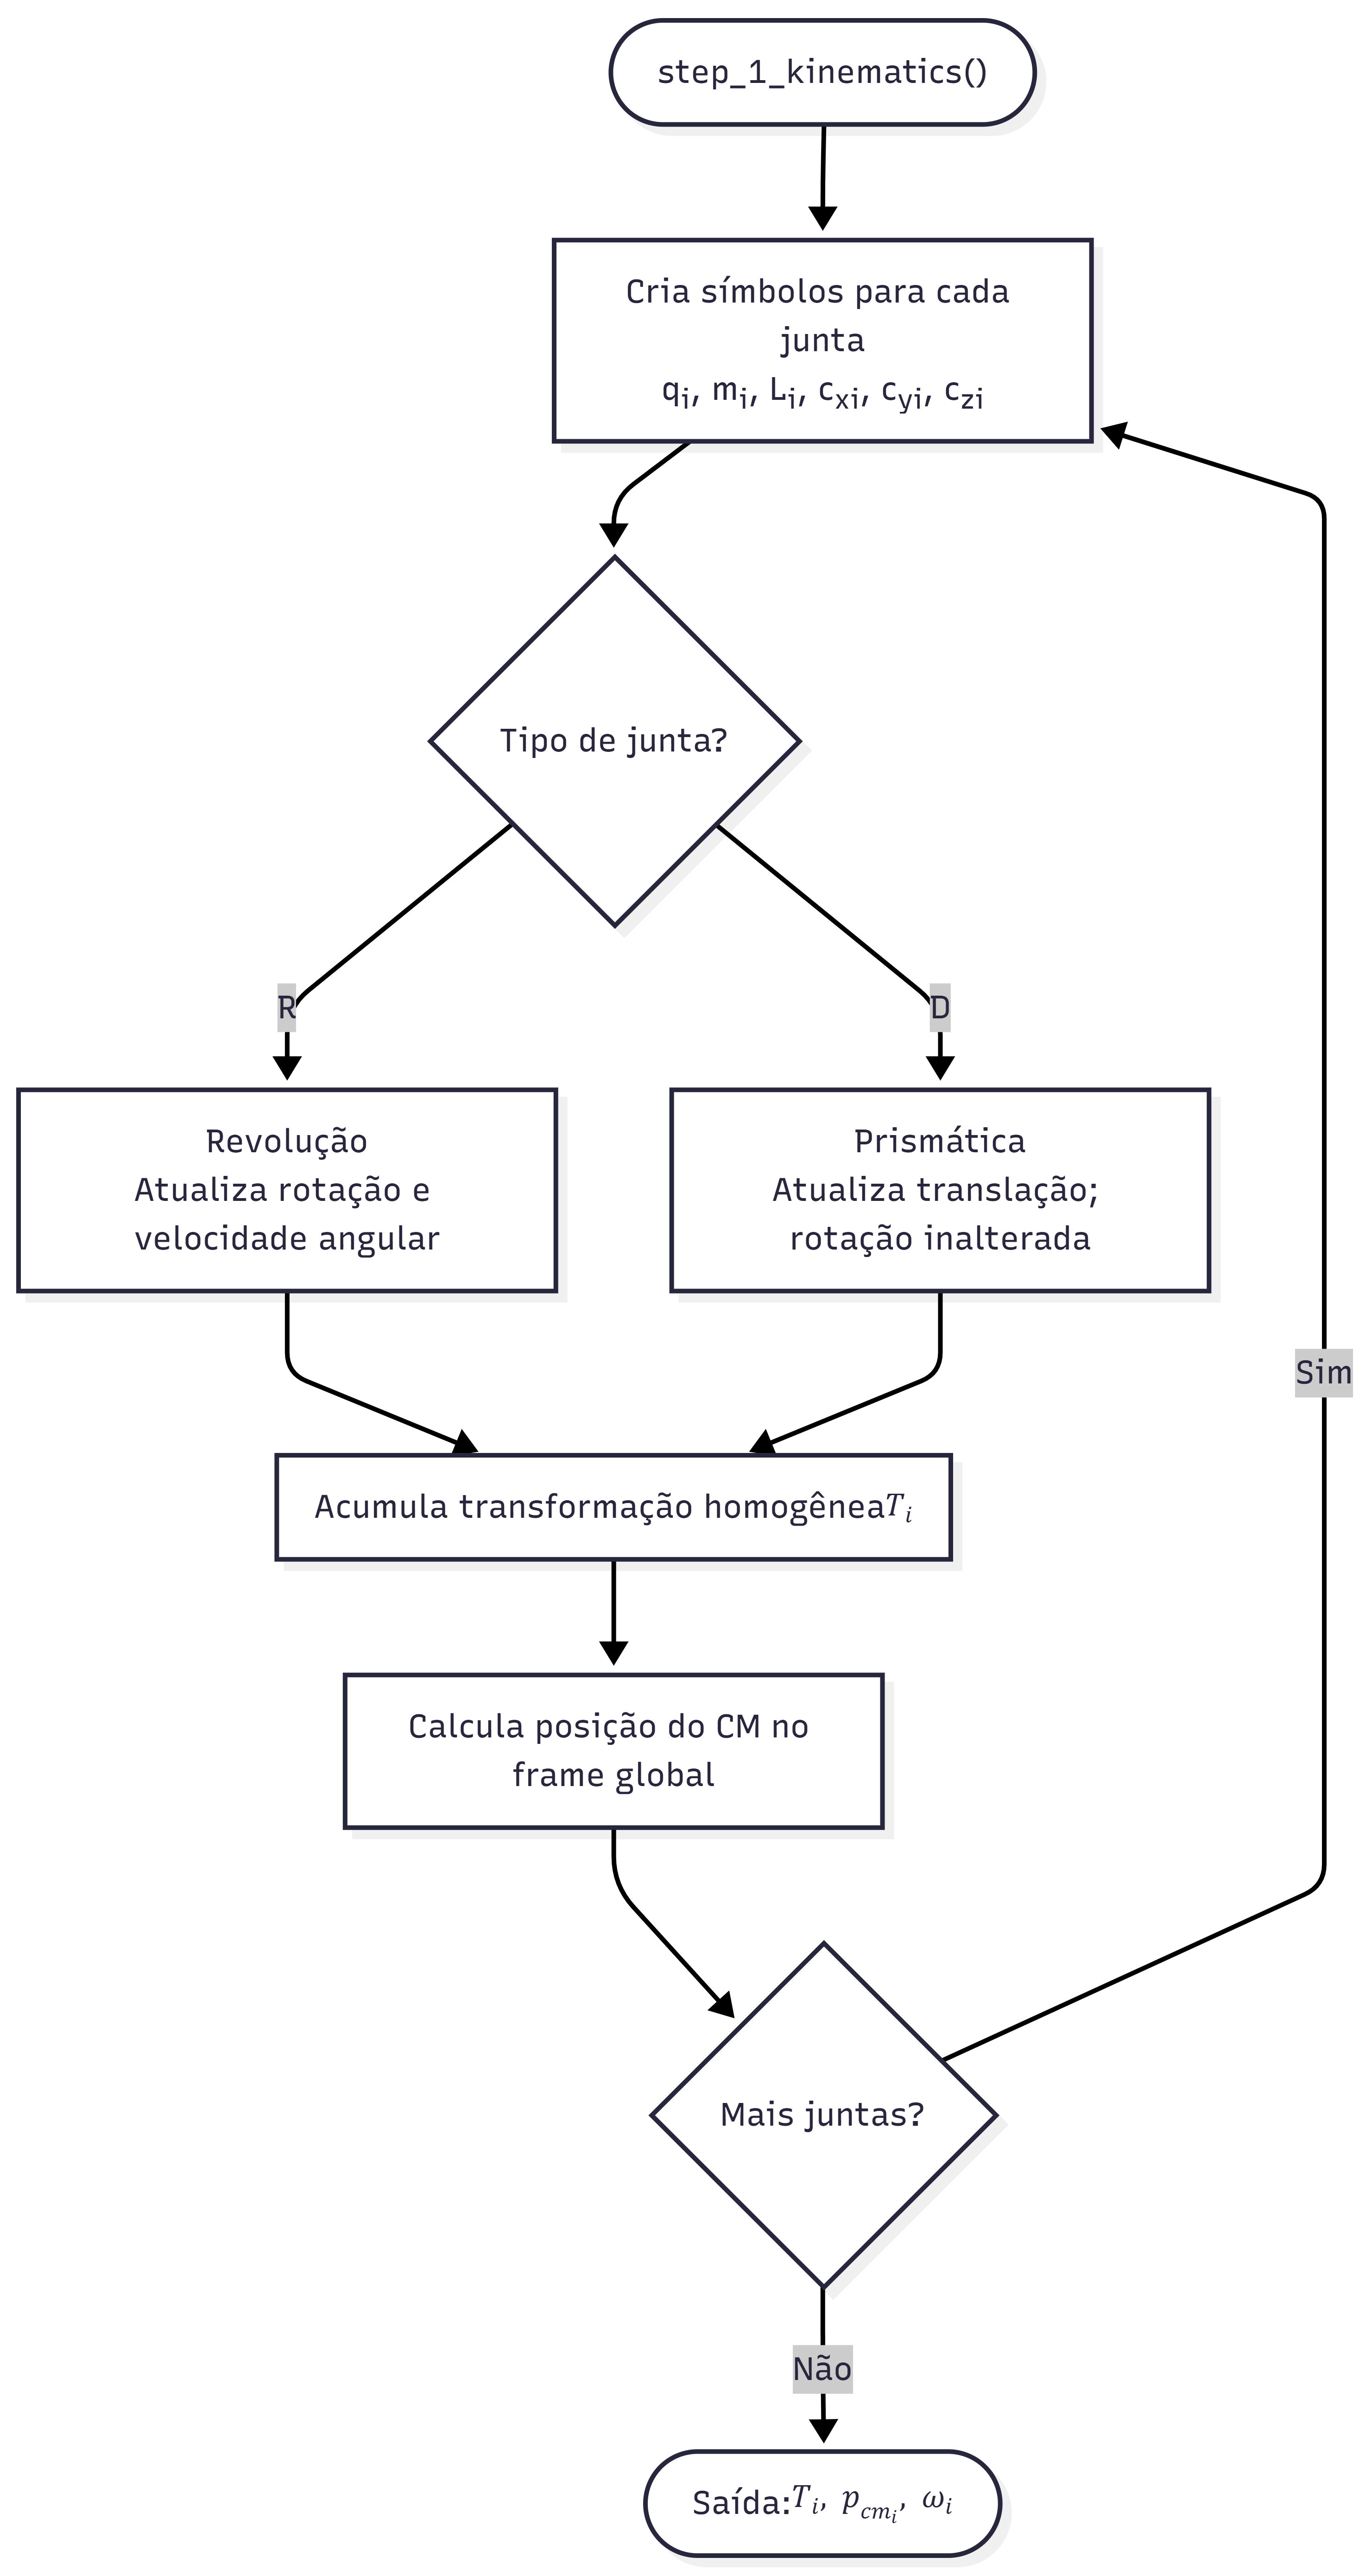
\includegraphics[width=0.70\textwidth]{figuras/Diagramas/Diagrama 2a — Cinemática Simbólica.png}
    \caption{Fluxo de cinemática simbólica implementado em \texttt{step\_1\_kinematics}: da especificação de \texttt{joint\_config} e \texttt{link\_vectors\_mask} à construção das transformações homogêneas acumuladas $T_i$, das posições dos centros de massa $\vec{p}_{\text{cm},i}$, das velocidades angulares $\vec{\omega}_i$ e do Jacobiano geométrico completo $J(q) \in \mathbb{R}^{6 \times N}$.}
    \label{fig:cinem_simbolica}
\end{figure}

% ==============================================================================
\section{Derivação Simbólica da Matriz de Inércia e do Vetor de Gravidade}
\label{sec:M_G}
% ==============================================================================

\subsection{Método do Jacobiano da Inércia}

A derivação da matriz de inércia generalizada $M(q)$ segue o método do Jacobiano da inércia \cite{siciliano2009robotics}, que expressa a energia cinética total como:
\begin{equation}
    T = \frac{1}{2}\dot{q}^\top M(q)\,\dot{q},
    \label{eq:T_total}
\end{equation}
onde:
\begin{itemize}
    \item $T \in \mathbb{R}$ é a energia cinética total do sistema;
    \item $\dot{q} \in \mathbb{R}^{N}$ é o vetor de velocidades generalizadas (uma componente por junta);
    \item $M(q) \in \mathbb{R}^{N\times N}$ é a matriz de inércia generalizada, simétrica e definida positiva;
    \item $N$ é o número de graus de liberdade da cadeia cinemática.
\end{itemize}

A matriz de inércia é construída pela soma das contribuições de cada elo:
\begin{equation}
    M(q) = \sum_{i=1}^{N} \left[ m_i\, J_{v,i}^\top\, J_{v,i} + J_{\omega,i}^\top\, I_i^{(g)}\, J_{\omega,i} \right].
    \label{eq:M_jacobian}
\end{equation}
onde:
\begin{itemize}
    \item $m_i \in \mathbb{R}$ é a massa do elo $i$;
    \item $J_{v,i} \in \mathbb{R}^{3\times N}$ é o Jacobiano de velocidade linear do centro de massa do elo $i$;
    \item $J_{\omega,i} \in \mathbb{R}^{3\times N}$ é o Jacobiano de velocidade angular do elo $i$;
    \item $I_i^{(g)} \in \mathbb{R}^{3\times 3}$ é o tensor de inércia do elo $i$ expresso no referencial global;
    \item $N$ é o número total de elos da cadeia.
\end{itemize}

Os Jacobianos de velocidade translacional e angular do CM do elo $i$ são obtidos diretamente por diferenciação simbólica:
\begin{equation}
    J_{v,i}(q) = \frac{\partial \vec{p}_{\text{cm},i}}{\partial q}, \qquad
    J_{\omega,i}(\dot{q}) = \frac{\partial \vec{\omega}_i}{\partial \dot{q}},
    \label{eq:jacobs}
\end{equation}
onde:
\begin{itemize}
    \item $J_{v,i}(q) \in \mathbb{R}^{3\times N}$ é o Jacobiano de velocidade linear do centro de massa do elo $i$;
    \item $J_{\omega,i}(\dot{q}) \in \mathbb{R}^{3\times N}$ é o Jacobiano de velocidade angular do elo $i$;
    \item $\vec{p}_{\text{cm},i} \in \mathbb{R}^{3}$ é a posição do CM do elo $i$ (Equação~\eqref{eq:pcm_global});
    \item $\vec{\omega}_i \in \mathbb{R}^{3}$ é a velocidade angular global do elo $i$ (Equação~\eqref{eq:omega_rec});
    \item $\partial/\partial q$ e $\partial/\partial \dot{q}$ denotam as derivadas parciais matriciais em relação aos vetores $q$ e $\dot{q}$.
\end{itemize}

Estas derivadas são computadas pelo método \texttt{.jacobian()} do SymPy. O tensor de inércia global $I_i^{(g)}$ é obtido pela transformação de Steiner:
\begin{equation}
    I_i^{(g)} = R_{\text{acc},i}\, I_i^{(l)}\, R_{\text{acc},i}^\top, \qquad
    I_i^{(l)} = \text{diag}(Ixx_i,\, Iyy_i,\, Izz_i),
    \label{eq:I_global}
\end{equation}
onde:
\begin{itemize}
    \item $I_i^{(g)} \in \mathbb{R}^{3\times 3}$ é o tensor de inércia do elo $i$ expresso no referencial global;
    \item $I_i^{(l)} \in \mathbb{R}^{3\times 3}$ é o tensor de inércia local, diagonal nas coordenadas principais do elo;
    \item $R_{\text{acc},i} \in \mathbb{R}^{3\times 3}$ é a matriz de rotação global acumulada até o elo $i$;
    \item $Ixx_i, Iyy_i, Izz_i$ são os momentos principais de inércia do elo no referencial local.
\end{itemize}
A hipótese de tensor diagonal em coordenadas principais locais , amplamente adotada quando os eixos de inércia são alinhados ao referencial de junta \cite{spong2020robot, siciliano2009robotics} , é suficiente para descrever elos com geometria simétrica.

\subsection{Vetor de Gradiente de Potencial Gravitacional}

A energia potencial total do sistema é:
\begin{equation}
    V(q) = \sum_{i=1}^{N} m_i\, g\, z_{\text{cm},i}(q),
    \label{eq:V_grav}
\end{equation}
onde:
\begin{itemize}
    \item $V(q) \in \mathbb{R}$ é a energia potencial gravitacional total do sistema;
    \item $m_i$ é a massa do elo $i$;
    \item $g$ é a aceleração da gravidade;
    \item $z_{\text{cm},i}(q)$ é a componente vertical (terceira coordenada) de $\vec{p}_{\text{cm},i}$, dependente da configuração $q$;
    \item $N$ é o número de elos.
\end{itemize}

O vetor de gravidade generalizada é então:
\begin{equation}
    G(q) = \left(\frac{\partial V}{\partial q}\right)^\top = \frac{\partial}{\partial q} \left[\sum_{i=1}^{N} m_i\, g\, z_{\text{cm},i}\right]^\top,
    \label{eq:G_vec}
\end{equation}
onde:
\begin{itemize}
    \item $G(q) \in \mathbb{R}^{N}$ é o vetor de torques generalizados devidos à gravidade;
    \item $\partial V/\partial q \in \mathbb{R}^{1\times N}$ é o gradiente da energia potencial em relação ao vetor de coordenadas generalizadas $q$;
    \item cada componente $G_i(q)$ representa o torque generalizado necessário para sustentar o peso estático do sistema na configuração $q$ \cite{craig1989introduction, spong2020robot};
    \item $(\cdot)^\top$ denota transposição, convertendo o gradiente-linha em vetor-coluna.
\end{itemize}
Esse vetor é computado pelo método \texttt{sp.Matrix([V\_tot]).jacobian(self.q).T}.

\subsection{Jacobiano Geométrico Completo}

O Jacobiano geométrico do efetuador $J(q) \in \mathbb{R}^{6 \times N}$ é montado pela concatenação das linhas translacionais (derivada da posição do extremo final em relação a $q$) com as linhas rotacionais (derivada de $\vec{\omega}_N$ em relação a $\dot{q}$):
\begin{equation}
    J(q) = \begin{bmatrix} J_{\text{lin}} \\ J_{\text{ang}} \end{bmatrix}, \quad
    J_{\text{lin}} = \frac{\partial\, \vec{p}_{\text{end}}}{\partial q} \in \mathbb{R}^{3 \times N}, \quad
    J_{\text{ang}} = \frac{\partial\, \vec{\omega}_N}{\partial \dot{q}} \in \mathbb{R}^{3 \times N}.
    \label{eq:jacobian_full}
\end{equation}
onde:
\begin{itemize}
    \item $J(q) \in \mathbb{R}^{6\times N}$ é o Jacobiano geométrico completo do efetuador;
    \item $J_{\text{lin}}$ é a parte linear, obtida pela derivada parcial da posição $\vec{p}_{\text{end}}$ do extremo final em relação a $q$;
    \item $J_{\text{ang}}$ é a parte angular, obtida pela derivada parcial da velocidade angular $\vec{\omega}_N$ do último elo em relação a $\dot{q}$;
    \item $\vec{p}_{\text{end}} \in \mathbb{R}^{3}$ é a posição cartesiana do efetuador no referencial global;
    \item $\vec{\omega}_N \in \mathbb{R}^{3}$ é a velocidade angular global do último elo da cadeia.
\end{itemize}

A disponibilidade do Jacobiano $6 \times N$ completo viabiliza o \emph{controle no espaço de tarefa 6D}, em que três coordenadas descrevem a \textbf{posição} cartesiana $(x, y, z)$ do efetuador e três coordenadas descrevem a sua \textbf{orientação} angular (\textit{roll}, \textit{pitch}, \textit{yaw}, ou, equivalentemente, o eixo-ângulo de uma rotação em $SO(3)$). As três primeiras linhas $J_{\text{lin}}$ projetam as velocidades de junta na velocidade linear do efetuador, enquanto as três últimas $J_{\text{ang}}$ as projetam na velocidade angular, totalizando seis graus de liberdade da tarefa cartesiana. Esta é uma extensão crítica em relação a abordagens que consideram apenas o Jacobiano posicional $3 \times N$, que são insuficientes para controle de orientação em tarefas de manipulação subaquática, soldagem, alinhamento com superfícies inclinadas ou inserção de peças, nas quais o ``onde'' (posição) e o ``como'' (orientação) do efetuador devem ser controlados simultaneamente \cite{chiaverini1997singularity, siciliano2009robotics}. O algoritmo de cinemática inversa em malha fechada que opera sobre este Jacobiano completo é detalhado na Seção~\ref{sec:clik_6d} do Capítulo~\ref{cap:simulacao}. O fluxo das Seções~\ref{sec:M_G} e~\ref{sec:cinematica_simbolica} é sintetizado na Figura~\ref{fig:dinam_simbolica}, na qual se evidencia como $M(q)$, $G(q)$ e $J(q)$ são derivados a partir das posições e Jacobianos de cada elo.

\begin{figure}[htbp]
    \centering
    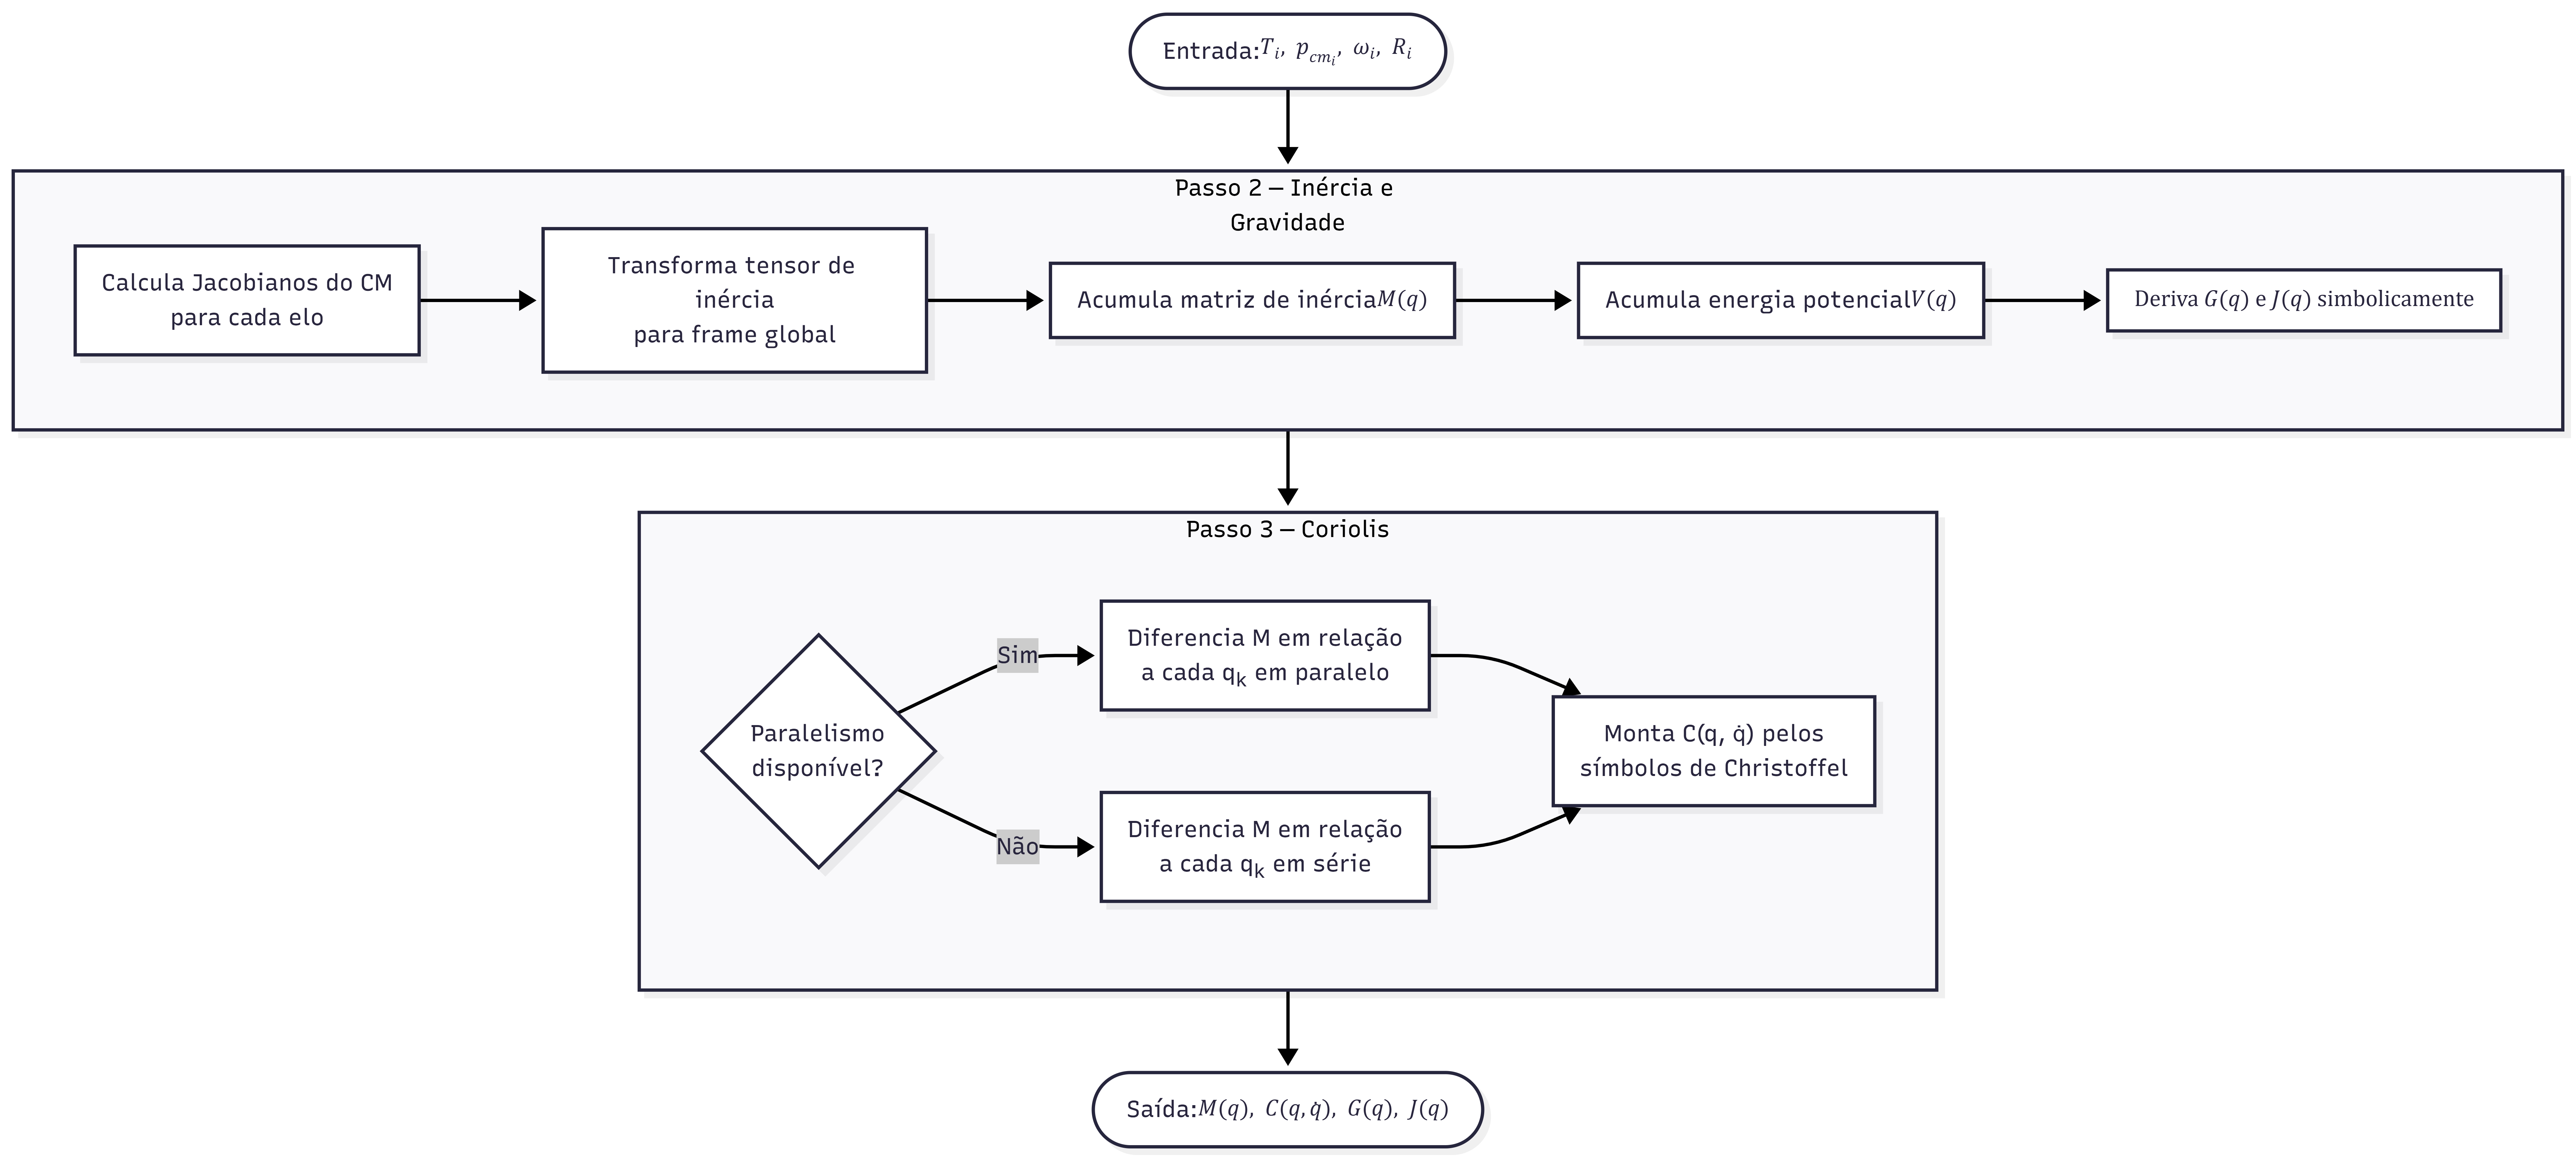
\includegraphics[width=0.92\textwidth]{figuras/Diagramas/Diagrama 2b — Dinâmica Simbólica M G e Coriolis.png}
    \caption{Fluxo de derivação simbólica da matriz de inércia $M(q)$, do vetor de gradiente de potencial $G(q)$ e dos coeficientes de Coriolis pelo método dos símbolos de Christoffel, implementado em \texttt{step\_2\_jacobian\_M\_G} e \texttt{step\_3\_coriolis\_combined}.}
    \label{fig:dinam_simbolica}
\end{figure}

% ==============================================================================
\section{Cálculo Simbólico do Vetor de Coriolis}
\label{sec:coriolis}
% ==============================================================================

\subsection{Formulação pelos Símbolos de Christoffel}

O vetor de termos de Coriolis e centrípetos $C(q,\dot{q}) \in \mathbb{R}^N$ é calculado pelos símbolos de Christoffel de segunda espécie \cite{spong2020robot, siciliano2009robotics}. Cada componente do vetor $C$ é:
\begin{equation}
    [C(q,\dot{q})]_i = \sum_{j=1}^{N}\sum_{k=j}^{N} c_{ijk}(q)\,\dot{q}_j\,\dot{q}_k \cdot \varepsilon_{jk},
    \label{eq:C_vec}
\end{equation}
onde:
\begin{itemize}
    \item $[C(q,\dot{q})]_i$ é a $i$-ésima componente do vetor de Coriolis;
    \item $c_{ijk}(q)$ são os símbolos de Christoffel de segunda espécie associados à matriz de inércia $M(q)$;
    \item $\dot{q}_j$ e $\dot{q}_k$ são velocidades generalizadas das juntas $j$ e $k$;
    \item $\varepsilon_{jk}$ é o coeficiente de simetria, com $\varepsilon_{jk} = 1$ se $j = k$ (termos centrípetos puros) e $\varepsilon_{jk} = 2$ se $j \neq k$ (termos de Coriolis cruzados);
    \item $N$ é o número de graus de liberdade.
\end{itemize}

Os coeficientes de Christoffel são:
\begin{equation}
    c_{ijk} = \frac{1}{2}\!\left(\frac{\partial M_{ij}}{\partial q_k} + \frac{\partial M_{ik}}{\partial q_j} - \frac{\partial M_{jk}}{\partial q_i}\right).
    \label{eq:christoffel_impl}
\end{equation}
onde:
\begin{itemize}
    \item $c_{ijk}(q) \in \mathbb{R}$ é o coeficiente de Christoffel de segunda espécie associado aos índices $(i,j,k)$;
    \item $M_{ij}, M_{ik}, M_{jk}$ são elementos da matriz de inércia $M(q)$;
    \item $\partial M_{ab}/\partial q_c$ é a derivada parcial do elemento $M_{ab}$ em relação à coordenada generalizada $q_c$.
\end{itemize}

Esta formulação é matematicamente equivalente às linhas $C_{ij}$ da matriz de Coriolis clássica (Equação~\eqref{eq:christoffel} do Capítulo~\ref{cap:revisao}), mas diretamente no formato vetorial $C(q,\dot{q})\dot{q}$, evitando a construção da matriz $N \times N$ completa , o que reduz o número total de operações de $O(N^3)$ para o cálculo dos coeficientes individuais sem custos adicionais de produto matriz-vetor.

A implementação segue dois sub-passos. No primeiro (\textit{Passo 3a}), a matriz de inércia $M$ é diferenciada em relação a cada variável de junta $q_k$, produzindo as matrizes $\partial M/\partial q_k \in \mathbb{R}^{N \times N}$ para $k = 1, \ldots, N$. No segundo (\textit{Passo 3b}), cada linha $i$ do vetor $C$ é montada pela varredura de todos os pares $(j, k)$ com $k \geq j$, utilizando as matrizes previamente calculadas. A exploração da simetria ($k \geq j$) reduz o número de pares de $N^2$ para $N(N+1)/2$ \cite{hollerbach1980recursive}.

\subsection{Estratégia de Paralelização da Derivação}

A derivação simbólica de $\partial M/\partial q_k$ é a operação mais custosa de toda a geração do modelo: em sistemas com $N$ graus de liberdade, cada um dos $N$ gradientes simbólicos exige a diferenciação de uma matriz $N \times N$ com entradas que podem possuir centenas de subexpressões, resultando em uma complexidade efetiva de $O(N^3)$ a $O(N^4)$ no tamanho das expressões para configurações gerais \cite{hollerbach1980recursive, leu1986automated}.

Para mitigar esse custo, o \textit{Hephaestus} distribui as $N$ tarefas de diferenciação $M \to \partial M/\partial q_k$ entre múltiplos processos via \texttt{ProcessPoolExecutor} da biblioteca padrão do Python:

\begin{equation}
    \texttt{dM\_dq}[k] = \frac{\partial M}{\partial q_k}, \quad k = 1, \ldots, N, \quad \text{computados em paralelo por } W \text{ \textit{workers}}.
    \label{eq:dMdq_parallel}
\end{equation}
onde:
\begin{itemize}
    \item $\texttt{dM\_dq}[k] \in \mathbb{R}^{N\times N}$ é a matriz de derivadas parciais $\partial M/\partial q_k$ armazenada na posição $k$ da lista resultante;
    \item $M \in \mathbb{R}^{N\times N}$ é a matriz de inércia simbólica completa;
    \item $q_k$ é a $k$-ésima coordenada generalizada;
    \item $N$ é o número de graus de liberdade;
    \item $W$ é o número de processos \textit{workers} alocados ao \texttt{ProcessPoolExecutor}.
\end{itemize}

O uso de processos (em vez de \textit{threads}) contorna a limitação do \textit{Global Interpreter Lock} (GIL) do CPython, que impede a execução simultânea de código Python puro em múltiplos \textit{threads} \cite{beazley2010understanding}. A serialização dos objetos simbólicos entre processos é viabilizada pela integração nativa do SymPy com o módulo \texttt{pickle} do Python, que representa expressões simbólicas como árvores de objetos serializáveis \cite{meurer2017sympy}.

Analogamente, o cálculo das $N$ linhas do vetor $C$ (cada linha requerendo $O(N^2)$ operações simbólicas sobre as matrizes $\partial M/\partial q_k$) é também paralelizado por \texttt{ProcessPoolExecutor}, com cada \textit{worker} responsável por uma linha $i$ do vetor:

\begin{equation}
    C_i = \sum_{j=1}^{N}\sum_{k=j}^{N} c_{ijk}\,\dot{q}_j\,\dot{q}_k \cdot \varepsilon_{jk}, \quad i = 1, \ldots, N, \quad \text{computados em paralelo}.
    \label{eq:C_parallel}
\end{equation}
onde:
\begin{itemize}
    \item $C_i$ é a $i$-ésima componente do vetor de Coriolis (cf.\ Equação~\eqref{eq:C_vec});
    \item $c_{ijk}$ são os coeficientes de Christoffel definidos pela Equação~\eqref{eq:christoffel_impl};
    \item $\dot{q}_j, \dot{q}_k$ são as velocidades generalizadas das juntas $j$ e $k$;
    \item $\varepsilon_{jk}$ é o coeficiente de simetria ($1$ ou $2$);
    \item $N$ é o número de graus de liberdade, e cada índice $i$ é processado por um \textit{worker} distinto.
\end{itemize}

Uma decisão de implementação relevante é a \emph{omissão intencional} da chamada a \texttt{sp.collect()} após a montagem de cada linha $C_i$. Embora a coleta de termos semelhantes possa compactar a expressão simbólica, seu custo computacional é superlinear no número de termos e pode superar em ordem de grandeza o custo do cálculo próprio da linha. Em vez disso, a compactação é delegada ao passo de CSE (\textit{Common Subexpression Elimination}) realizado posteriormente no \texttt{lambdify}, que fatoriza subexpressões repetidas de forma sistemática e com custo linear no tamanho da expressão final \cite{alfred2007compilers, meurer2017sympy}.

\subsection{Modo Serial para Ambientes Executáveis}

Quando o \textit{Hephaestus} é distribuído como executável via PyInstaller (arquivo \texttt{.exe}), o suporte ao \textit{spawn} de subprocessos no Windows impõe restrições de inicialização que tornam o \texttt{ProcessPoolExecutor} incompatível com módulos congelados (\textit{frozen}). Nesse cenário, o número de \textit{workers} é automaticamente configurado para 1, e a computação é realizada em série na mesma \textit{thread} principal. Essa detecção é realizada pelo parâmetro \texttt{num\_workers} da classe \texttt{RobotMathEngine}: quando \texttt{num\_workers = 1}, a condição \texttt{use\_parallel = False} desativa o executor, garantindo execução correta em qualquer ambiente sem modificações no código \cite{leu1986automated}.

% ==============================================================================
\section{Extensão Hidrodinâmica: \texttt{RobotMathHydro}}
\label{sec:hydro_engine}
% ==============================================================================

A classe \texttt{RobotMathHydro} herda integralmente de \texttt{RobotMathEngine} e sobrescreve os métodos \texttt{step\_1\_kinematics\_hydro} e \texttt{step\_2\_jacobian\_M\_G} para incorporar os efeitos físicos do ambiente aquático, conforme a formulação de Fossen \cite{fossen2011handbook} e Antonelli \cite{antonelli2014modelling}.

\subsection{Parâmetros Adicionais: Volumes e Massa Adicionada}

No passo de cinemática hidrodinâmica, após a execução completa de \texttt{step\_1\_kinematics}, são acrescentados à lista de parâmetros os volumes deslocados $\text{vol}_i$ de cada elo ($i = 1, \ldots, N$). Esses volumes determinam a força de empuxo por elo segundo o princípio de Arquimedes:
\begin{equation}
    B_i = \rho\, g\, \text{vol}_i,
    \label{eq:empuxo_por_elo}
\end{equation}
onde:
\begin{itemize}
    \item $B_i$ é o módulo da força de empuxo aplicada ao elo $i$;
    \item $\rho$ é a densidade do fluido (no caso típico, água do mar) \cite{newman1977marine};
    \item $g$ é a aceleração da gravidade;
    \item $\text{vol}_i$ é o volume submerso deslocado pelo elo $i$.
\end{itemize}

No passo de dinâmica hidrodinâmica, os coeficientes de massa adicionada de cada elo são instanciados como seis símbolos escalares:
\begin{equation}
    \{ma_{u,i},\, ma_{v,i},\, ma_{w,i}\} \quad \text{(translacionais)}, \qquad
    \{ma_{p,i},\, ma_{q,i},\, ma_{r,i}\} \quad \text{(rotacionais)},
    \label{eq:MA_syms}
\end{equation}
onde:
\begin{itemize}
    \item $ma_{u,i}, ma_{v,i}, ma_{w,i}$ são os coeficientes de massa adicionada translacionais nas direções $u$ (\textit{surge}), $v$ (\textit{sway}) e $w$ (\textit{heave}) do elo $i$, no referencial local;
    \item $ma_{p,i}, ma_{q,i}, ma_{r,i}$ são os coeficientes de massa adicionada rotacionais em torno dos eixos $p$ (\textit{roll}), $q$ (\textit{pitch}) e $r$ (\textit{yaw}) do elo $i$, no referencial local;
    \item o índice $i$ percorre todos os elos da cadeia ($i = 1, \ldots, N$).
\end{itemize}

Esses símbolos formam as matrizes diagonais locais $M_{A,\text{lin},i}^{(l)} = \text{diag}(ma_{u,i}, ma_{v,i}, ma_{w,i})$ e $M_{A,\text{rot},i}^{(l)} = \text{diag}(ma_{p,i}, ma_{q,i}, ma_{r,i})$. A parametrização diagonal é adequada para corpos com pelo menos um plano de simetria geométrica, condição satisfeita pela grande maioria dos elos de UVMSs comerciais \cite{fossen2011handbook}.

\subsection{Matriz de Inércia com Massa Adicionada}

A matriz de inércia generalizada no modo subaquático é:
\begin{equation}
    M_{\text{Hydro}}(q) = \sum_{i=1}^{N} \left[
        J_{v,i}^\top \left(m_i I_3 + M_{A,\text{lin},i}^{(g)}\right) J_{v,i}
        + J_{\omega,i}^\top \left(I_i^{(g)} + M_{A,\text{rot},i}^{(g)}\right) J_{\omega,i}
    \right],
    \label{eq:M_hydro_impl}
\end{equation}
onde:
\begin{itemize}
    \item $M_{\text{Hydro}}(q) \in \mathbb{R}^{N\times N}$ é a matriz de inércia generalizada no modo subaquático;
    \item $m_i$ é a massa do elo $i$ e $I_3$ é a matriz identidade $3\times 3$;
    \item $M_{A,\text{lin},i}^{(g)} \in \mathbb{R}^{3\times 3}$ é a matriz diagonal de massa adicionada translacional do elo $i$ no referencial global;
    \item $M_{A,\text{rot},i}^{(g)} \in \mathbb{R}^{3\times 3}$ é a matriz diagonal de massa adicionada rotacional do elo $i$ no referencial global;
    \item $I_i^{(g)} \in \mathbb{R}^{3\times 3}$ é o tensor de inércia rígida do elo $i$ no referencial global (Equação~\eqref{eq:I_global});
    \item $J_{v,i}, J_{\omega,i} \in \mathbb{R}^{3\times N}$ são os Jacobianos linear e angular do elo $i$ (Equação~\eqref{eq:jacobs}).
\end{itemize}

As matrizes de massa adicionada globais são obtidas pela transformação pelo referencial acumulado:
\begin{equation}
    M_{A,\text{lin},i}^{(g)} = R_{\text{acc},i}\, M_{A,\text{lin},i}^{(l)}\, R_{\text{acc},i}^\top, \qquad
    M_{A,\text{rot},i}^{(g)} = R_{\text{acc},i}\, M_{A,\text{rot},i}^{(l)}\, R_{\text{acc},i}^\top.
    \label{eq:MA_global}
\end{equation}
onde:
\begin{itemize}
    \item $M_{A,\text{lin},i}^{(l)}, M_{A,\text{rot},i}^{(l)} \in \mathbb{R}^{3\times 3}$ são as matrizes diagonais de massa adicionada translacional e rotacional no referencial local do elo $i$ (Equação~\eqref{eq:MA_syms});
    \item $R_{\text{acc},i} \in \mathbb{R}^{3\times 3}$ é a matriz de rotação global acumulada até o elo $i$;
    \item a transformação $R\,(\cdot)\,R^\top$ realiza a mudança de base de tensores de segunda ordem do referencial local para o global.
\end{itemize}

A Equação~\eqref{eq:M_hydro_impl} expande a Equação~\eqref{eq:M_jacobian} pelo princípio de superposição da inércia virtual \cite{fossen2011handbook}: a massa adicionada $M_{A,i}$ representa a inércia do fluido acelerado pelo movimento do elo $i$, projetada no espaço de juntas via Jacobianos, exatamente como a inércia rígida do próprio elo. Essa equivalência formal permite a reutilização do mesmo \textit{framework} de derivação de $M$ para ambos os cenários (ar e água), com mínima duplicação de código.

\subsection{Vetor de Potencial Aparente: Peso menos Empuxo}

A energia potencial aparente de cada elo submerso combina o potencial gravitacional com o trabalho da força de empuxo:
\begin{equation}
    V_i^{\text{app}}(q) = (m_i - \rho\, \text{vol}_i)\, g\, z_{\text{cm},i}(q),
    \label{eq:V_aparente}
\end{equation}
onde:
\begin{itemize}
    \item $V_i^{\text{app}}(q)$ é a energia potencial aparente (peso menos empuxo) do elo $i$;
    \item $m_i$ é a massa do elo $i$ e $\rho\, \text{vol}_i$ é a massa de fluido deslocada pelo elo;
    \item $g$ é a aceleração da gravidade;
    \item $z_{\text{cm},i}(q)$ é a coordenada vertical do CM do elo $i$;
    \item conforme definido na Equação~\eqref{eq:buoyancy_potential} do Capítulo~\ref{cap:revisao}.
\end{itemize}

O vetor $G_{\text{Hydro}}(q)$ resultante é o gradiente desta soma:
\begin{equation}
    G_{\text{Hydro}}(q) = \left(\frac{\partial}{\partial q} \sum_{i=1}^{N} (m_i - \rho\, \text{vol}_i)\,g\,z_{\text{cm},i}\right)^\top.
    \label{eq:G_hydro}
\end{equation}
onde:
\begin{itemize}
    \item $G_{\text{Hydro}}(q) \in \mathbb{R}^{N}$ é o vetor de torques generalizados aparentes (gravidade menos empuxo);
    \item os demais símbolos seguem a Equação~\eqref{eq:V_aparente};
    \item $(\cdot)^\top$ converte o gradiente-linha em vetor-coluna.
\end{itemize}

Quando $m_i \approx \rho\, \text{vol}_i$ (elo neutralmente flutuante), $V_i^{\text{app}} \approx 0$ e o correspondente torque estático $G_i(q)$ anula-se, reproduzindo o cenário típico de UVMSs projetados para equilíbrio neutro que minimizam o esforço estático dos atuadores \cite{antonelli2014modelling, yuh2001underwater}.

\subsection{Modelo Dinâmico Unificado}

A estrutura formal das equações de movimento hidrodinâmicas é idêntica à terrestre:
\begin{equation}
    M_{\text{Hydro}}(q)\ddot{q} + C_{\text{Hydro}}(q,\dot{q})\dot{q} + G_{\text{Hydro}}(q) = \tau,
    \label{eq:EOM_hydro}
\end{equation}
onde:
\begin{itemize}
    \item $M_{\text{Hydro}}(q) \in \mathbb{R}^{N\times N}$ é a matriz de inércia generalizada aparente (Equação~\eqref{eq:M_hydro_impl});
    \item $C_{\text{Hydro}}(q,\dot{q}) \in \mathbb{R}^{N\times N}$ é a matriz de Coriolis e termos centrípetos calculada pelos mesmos símbolos de Christoffel sobre $M_{\text{Hydro}}$ (Equação~\eqref{eq:christoffel_impl}), sem nenhuma modificação algorítmica;
    \item $G_{\text{Hydro}}(q) \in \mathbb{R}^{N}$ é o vetor de torques generalizados aparentes (Equação~\eqref{eq:G_hydro});
    \item $q, \dot{q}, \ddot{q} \in \mathbb{R}^{N}$ são os vetores de posições, velocidades e acelerações generalizadas;
    \item $\tau \in \mathbb{R}^{N}$ é o vetor de torques generalizados aplicados pelos atuadores.
\end{itemize} Os termos de arrasto hidrodinâmico $\tau_{\text{drag}} = D_{\text{lin}}\dot{q} + D_{\text{quad}}|\dot{q}|\dot{q}$ (Equação~\eqref{eq:drag} do Capítulo~\ref{cap:revisao}) são aplicados separadamente no integrador numérico como forças passivas, não na geração simbólica do modelo, pela razão de que sua forma $|\dot{q}_i|\dot{q}_i$ não é simbólica no sentido lagrangiano clássico \cite{fossen2011handbook}. Ilustra-se, na Figura~\ref{fig:hydro_extensao}, como \texttt{RobotMathHydro} estende \texttt{RobotMathEngine} por herança, sobrescrevendo os métodos de dinâmica para incorporar massa adicionada e potencial aparente Peso--Empuxo.

\begin{figure}[htbp]
    \centering
    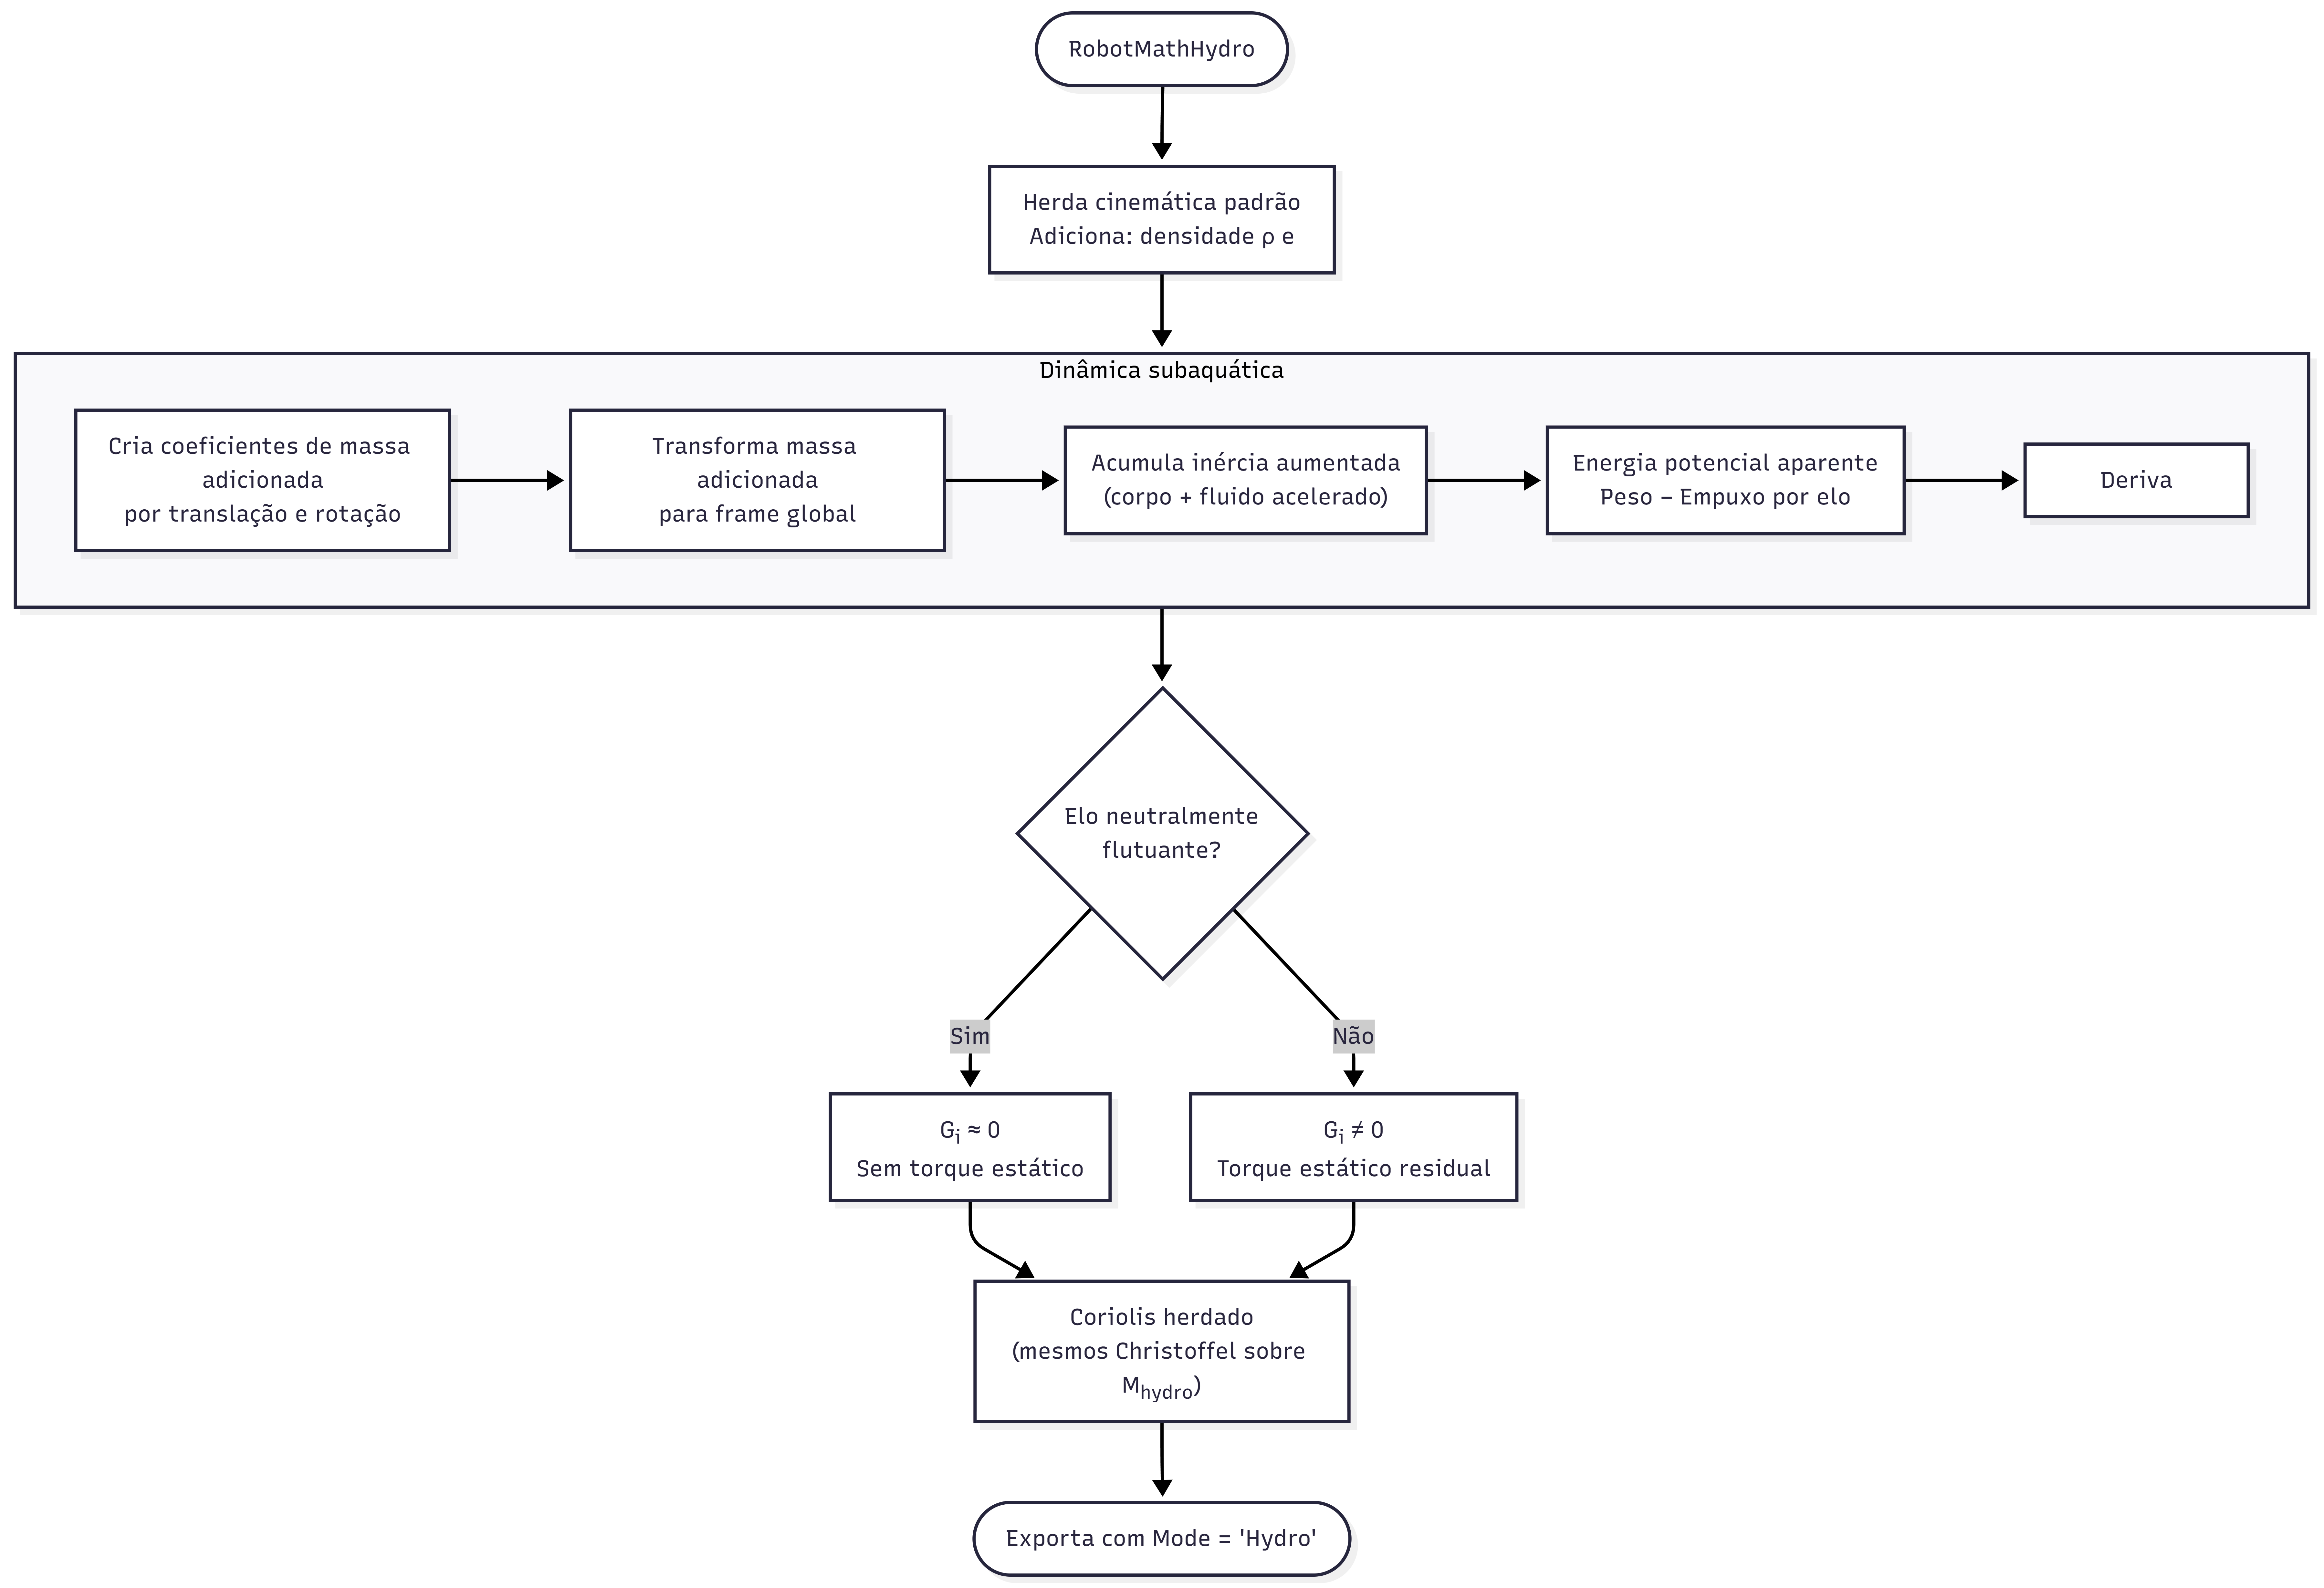
\includegraphics[width=1\textwidth]{figuras/Diagramas/Diagrama 3 — Extensão Hidrodinâmica.png}
    \caption{Extensão hidrodinâmica implementada em \texttt{RobotMathHydro}: herança de \texttt{RobotMathEngine} com sobrescrita dos métodos de cinemática e dinâmica para incorporar o tensor de massa adicionada $M_A^{(g)}$ (Equação~\eqref{eq:M_hydro_impl}) e o potencial aparente Peso--Empuxo (Equação~\eqref{eq:V_aparente}) segundo a formulação de Fossen~\cite{fossen2011handbook}.}
    \label{fig:hydro_extensao}
\end{figure}

% ==============================================================================
\section{Preparação e Exportação do Modelo Simbólico}
\label{sec:export}
% ==============================================================================

\subsection{Substituição de Símbolos Dinâmicos}

O método \texttt{step\_4\_prepare\_export} realiza a substituição dos \texttt{dynamicsymbols} dependentes do tempo , $q_i(t)$ e $\dot{q}_i(t)$ , por símbolos escalares estáticos $q_i$ e $\dot{q}_i$, via o mapeamento:
\begin{equation}
    q_i(t) \mapsto \texttt{sp.Symbol}(f\text{'q\{i\}'}), \qquad
    \dot{q}_i(t) \mapsto \texttt{sp.Symbol}(f\text{'dq\{i\}'}).
    \label{eq:subs_dynamic}
\end{equation}
onde:
\begin{itemize}
    \item $q_i(t)$ é a função simbólica dependente do tempo, criada via \texttt{dynamicsymbols} do SymPy;
    \item $\dot{q}_i(t) = dq_i(t)/dt$ é sua derivada temporal simbólica;
    \item $\mapsto$ representa a substituição da função do tempo por um símbolo escalar livre;
    \item $\texttt{sp.Symbol}(\cdot)$ é o construtor de símbolos escalares estáticos do SymPy;
    \item $f\text{'q\{i\}'}$ e $f\text{'dq\{i\}'}$ são os nomes \textit{formatados} das variáveis estáticas (e.g., \texttt{q1}, \texttt{dq1}, \texttt{q2}, \ldots).
\end{itemize}

Esse passo é necessário porque \texttt{dynamicsymbols} são, internamente, funções do tempo no SymPy, e sua presença nas expressões interfere com o \texttt{lambdify} , que espera símbolos escalares como variáveis de entrada \cite{meurer2017sympy}. A substituição não altera a estrutura algébrica das expressões; apenas troca a representação interna de ``função aplicada'' para ``símbolo livre''.

\subsection{Exportação do Dicionário de Resultados}

O método retorna um dicionário com as seguintes chaves:

\begin{itemize}
    \item \texttt{"M"}: a matriz de inércia $M(q) \in \mathbb{R}^{N \times N}$, expressa nos símbolos estáticos;
    \item \texttt{"G"}: o vetor de gradiente de potencial $G(q) \in \mathbb{R}^N$;
    \item \texttt{"C"}: o vetor de Coriolis $C(q,\dot{q}) \in \mathbb{R}^N$ (já no formato $C(q,\dot{q})\dot{q}$);
    \item \texttt{"J"}: o Jacobiano geométrico $J(q) \in \mathbb{R}^{6 \times N}$;
    \item \texttt{"FK\_Pos"}: a transformação homogênea completa do efetuador final $T_N(q)$;
    \item \texttt{"FK\_Vel"}: a velocidade cartesiana do efetuador $J(q)\dot{q}$;
    \item \texttt{"Subs"}: o mapeamento de substituição (Equação~\eqref{eq:subs_dynamic});
    \item \texttt{"Mode"}: string \texttt{"Air"} ou \texttt{"Hydro"}, para controle de fluxo no simulador.
\end{itemize}

Essa interface de exportação desacopla completamente a \textit{engine} matemática do módulo de simulação, permitindo que o modelo simbólico seja serializado (via \texttt{pickle}) e reutilizado em sessões posteriores sem recomputação , uma funcionalidade de produtividade crítica, dado que a geração do modelo para sistemas com $N \geq 6$ pode levar dezenas de minutos em \textit{hardware} convencional \cite{leu1986automated, hollerbach1980recursive}.

% ==============================================================================
\section{Compilação Simbólico-Numérica com \texttt{lambdify} e CSE}
\label{sec:lambdify_cse}
% ==============================================================================

\subsection{A Interface \texttt{lambdify}}

A transição das expressões simbólicas para funções numéricas avaliáveis é o passo de maior impacto sobre o desempenho computacional da simulação. O SymPy fornece a função \texttt{sp.lambdify()} para esse propósito: dado um conjunto de variáveis simbólicas $\{v_1, \ldots, v_k\}$ e uma expressão (ou matriz) simbólica $\mathcal{E}(v_1,\ldots,v_k)$, \texttt{lambdify} gera o código-fonte Python/NumPy equivalente e compila-o via \texttt{exec}, retornando uma função numérica de alta performance \cite{meurer2017sympy}.

No \textit{Hephaestus}, a assinatura do \texttt{lambdify} é:
\begin{equation}
    f_{M,C,G,J}(q_1,\ldots,q_N,\,\dot{q}_1,\ldots,\dot{q}_N,\,g,\,m_1,\,L_1,\,cx_1,\ldots) \to \mathbb{R}^{\cdot \times \cdot},
    \label{eq:lambdify_signature}
\end{equation}
onde:
\begin{itemize}
    \item $f_{M,C,G,J}$ representa cada uma das funções numéricas compiladas (uma para $M$, $C$, $G$ e $J$);
    \item $q_1, \ldots, q_N$ são as coordenadas generalizadas (entradas dinâmicas);
    \item $\dot{q}_1, \ldots, \dot{q}_N$ são as velocidades generalizadas;
    \item $g$ é a aceleração da gravidade;
    \item $m_1, L_1, cx_1, \ldots$ representam os parâmetros físicos (massa, comprimento, coordenadas do CM, momentos de inércia etc.) listados em \texttt{params\_list};
    \item $\mathbb{R}^{\cdot \times \cdot}$ denota a saída numérica, cuja dimensão depende da grandeza avaliada (e.g., $N\times N$ para $M$, $N$ para $G$, $6\times N$ para $J$).
\end{itemize}
Essa assinatura corresponde à lista \texttt{sym\_vars = bot.q + bot.dq + bot.params\_list}, e garante que a mesma assinatura seja utilizada para todas as funções compiladas ($M$, $C$, $G$, $J$, FK), simplificando o gerenciamento de argumentos no \textit{loop} de simulação.

\subsection{Eliminação de Subexpressões Comuns}

O parâmetro \texttt{cse=True} ativa a Eliminação de Subexpressões Comuns (\textit{Common Subexpression Elimination}, CSE) antes da geração do código numérico \cite{alfred2007compilers}. Internamente, o SymPy aplica o algoritmo de Risch-Moses para CSE \cite{moses1971algebraic}, identificando subárvores repetidas na expressão simbólica e substituindo cada ocorrência por uma variável temporária. O código Python gerado tem então a forma:

\begin{align}
    &\texttt{x0} = \sin(q_1), \quad \texttt{x1} = \cos(q_1), \quad \texttt{x2} = \texttt{x0} \cdot m_1, \quad \ldots \nonumber \\
    &M[0,0] = \texttt{x2} \cdot L_1^2 + \ldots, \quad M[0,1] = \texttt{x1} \cdot \texttt{x2} + \ldots
    \label{eq:cse_example}
\end{align}
onde:
\begin{itemize}
    \item $\texttt{x0}, \texttt{x1}, \texttt{x2}, \ldots$ são variáveis temporárias geradas pelo CSE para subexpressões repetidas;
    \item $\sin(q_1), \cos(q_1)$ são funções trigonométricas elementares avaliadas uma única vez por passo;
    \item $m_1, L_1$ são parâmetros físicos do primeiro elo (massa e comprimento);
    \item $M[0,0], M[0,1]$ são elementos da matriz de inércia compilada, expressos em função das variáveis temporárias e dos parâmetros físicos.
\end{itemize}

O impacto quantitativo da CSE é substancial: para um manipulador de 6 GDL em ar, a expressão simbólica de $M(q)$ pode conter $O(10^3)$ a $O(10^4)$ operações primitivas; com CSE, a função compilada executa tipicamente $2$--$5\times$ mais rápido, com redução de $60$--$90\%$ no tamanho do \textit{bytecode} \cite{meurer2017sympy, alfred2007compilers}. Para sistemas maiores ($N > 8$), a CSE pode ser a diferença entre uma compilação que produz código de tamanho manejável e uma que gera \textit{strings} de vários MB que excedem os limites de compilação do Python (\texttt{MemoryError}) \cite{leu1986automated}.

Adicionalmente, o módulo \texttt{modules='numpy'} instrui o \texttt{lambdify} a mapear funções simbólicas (\texttt{sp.sin}, \texttt{sp.cos}, etc.) para suas contrapartes NumPy (\texttt{np.sin}, \texttt{np.cos}), que por sua vez invocam implementações C compiladas via BLAS/LAPACK \cite{meurer2017sympy}. O resultado é uma função numérica que se comporta como código C nativo para as operações de ponto flutuante, sem o \textit{overhead} da álgebra simbólica em tempo de simulação.

\subsection{Compilação das Funções por Módulo}

No construtor \texttt{RobotSimulator.\_\_init\_\_}, cada grandeza dinâmica é compilada individualmente, produzindo quatro funções distintas:

\begin{itemize}
    \item \texttt{func\_M}: $f_M: \mathbb{R}^{2N+P} \to \mathbb{R}^{N \times N}$, avalia a matriz de inércia;
    \item \texttt{func\_C}: $f_C: \mathbb{R}^{2N+P} \to \mathbb{R}^{N}$, avalia o vetor de Coriolis;
    \item \texttt{func\_G}: $f_G: \mathbb{R}^{2N+P} \to \mathbb{R}^{N}$, avalia o gradiente de potencial;
    \item \texttt{func\_J}: $f_J: \mathbb{R}^{2N+P} \to \mathbb{R}^{6 \times N}$, avalia o Jacobiano completo;
    \item \texttt{funcs\_fk\_all\_links}: lista de $N$ funções $f_{\text{FK},i}: \mathbb{R}^{2N+P} \to \mathbb{R}^{3}$, avaliando a posição 3D do extremo do elo $i$ , utilizadas para a visualização gráfica animada do manipulador.
\end{itemize}

onde $P = |\texttt{params\_list}|$ é o número total de parâmetros físicos. A compilação separada por grandeza , em vez de uma única função monolítica , permite o despacho paralelo de $M$, $C$ e $G$ durante a simulação: cada uma das funções pode ser submetida simultaneamente a um \textit{worker} distinto do executor paralelo, triplicando a taxa de avaliação dinâmica em máquinas com pelo menos três núcleos \cite{leu1986automated}. Sintetiza-se, na Figura~\ref{fig:compilacao_simbolica}, o fluxo completo de compilação simbólico-numérica, desde as expressões SymPy geradas nas etapas anteriores até as funções NumPy prontas para avaliação a cada passo de integração.

\begin{figure}[htbp]
    \centering
    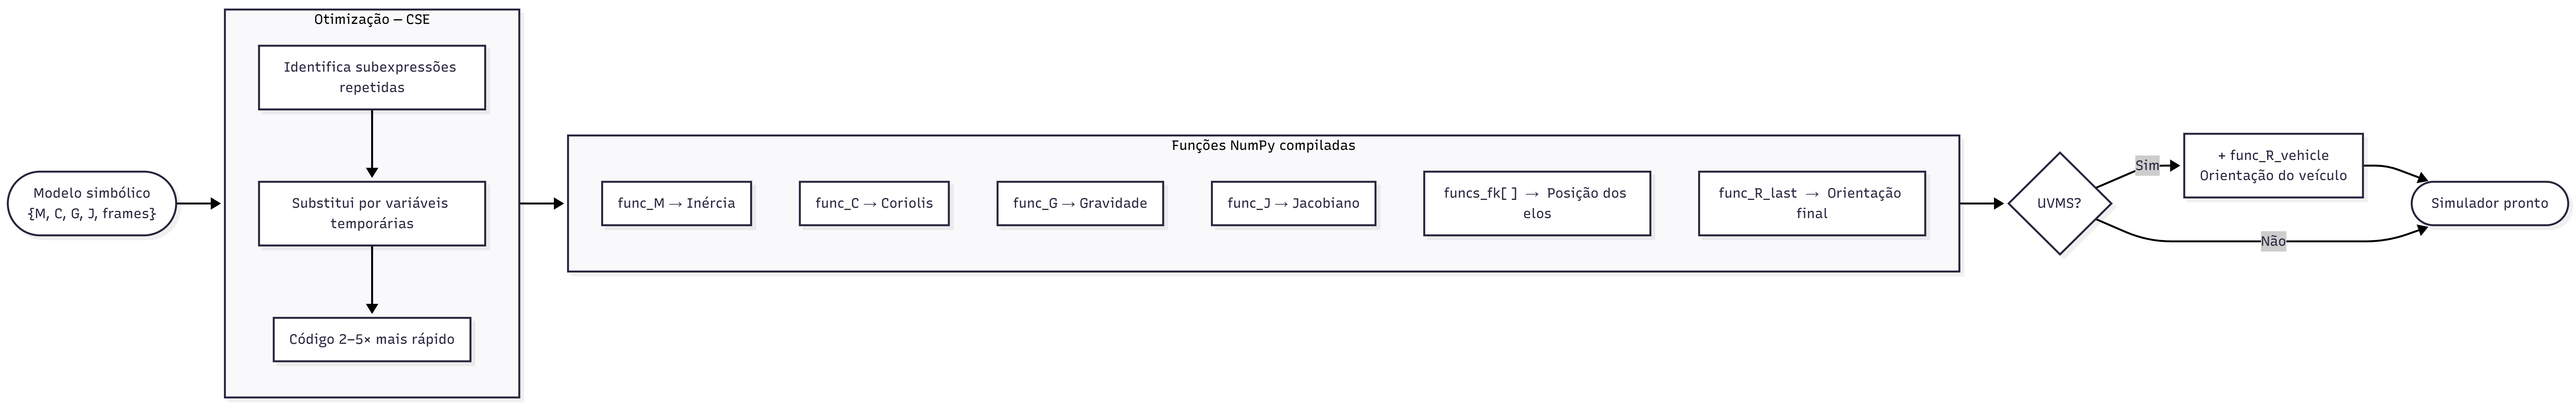
\includegraphics[width=0.92\textwidth]{figuras/Diagramas/Diagrama 4 — Compilação Simbólico-Numérica.png}
    \caption{Fluxo de compilação simbólico-numérica via \texttt{sp.lambdify()} com CSE ativo: as expressões SymPy de $M$, $C$, $G$ e $J$ passam pela Eliminação de Subexpressões Comuns antes de gerar código Python/NumPy compilado, reduzindo em 60--90\% o número de operações primitivas e viabilizando a avaliação em tempo de simulação \cite{meurer2017sympy, alfred2007compilers}.}
    \label{fig:compilacao_simbolica}
\end{figure}

% ==============================================================================
\section{Paralelismo em Dois Níveis e Executor Persistente}
\label{sec:parallel}
% ==============================================================================

O \textit{Hephaestus} implementa paralelismo em dois níveis distintos, correspondentes às duas fases temporalmente separadas do fluxo de trabalho:

\subsection{Nível 1: Paralelismo na Derivação Simbólica}

Como descrito na Seção~\ref{sec:coriolis}, o cálculo de $\partial M/\partial q_k$ e das linhas de $C$ é distribuído entre múltiplos processos durante a fase de \emph{geração do modelo} (executada uma única vez). O custo de \textit{spawn} dos processos e da serialização das expressões simbólicas é amortizado pelo ganho de velocidade na derivação, sendo lucrativo quando $N \geq 4$ e $W \geq 2$ processos estão disponíveis \cite{hollerbach1980recursive, beazley2010understanding}.

\subsection{Nível 2: Paralelismo na Avaliação Numérica}

Durante a fase de \emph{simulação}, as funções \texttt{func\_M}, \texttt{func\_C} e \texttt{func\_G} são avaliadas numericamente a cada passo de integração física (tipicamente $\Delta t = 10^{-3}$ s, correspondendo a 1000 avaliações por segundo de simulação). Para evitar o custo de \textit{respawn} de processos a cada avaliação , que, em testes, somava 2-8 segundos por simulação , o \textit{Hephaestus} utiliza um \textbf{executor persistente} (\texttt{ProcessPoolExecutor} pré-inicializado):

\begin{itemize}
    \item O executor é instanciado \emph{uma única vez} após a compilação, por meio do método \texttt{warm\_up\_workers()}, e mantido ativo durante toda a vida do objeto \texttt{RobotSimulator};
    \item Cada \textit{worker} executa o \textit{inicializador} \texttt{\_init\_worker}, que compila localmente as expressões simbólicas (via \texttt{lambdify}) e armazena as funções no dicionário de módulo \texttt{\_WORKER\_FUNCS};
    \item A cada passo de simulação, três tarefas são submetidas ao executor em paralelo , \texttt{("M", args)}, \texttt{("C", args)}, \texttt{("G", args)} , e os resultados são coletados por \texttt{Future.result()};
    \item O executor é encerrado explicitamente pelo método \texttt{close()}, chamado automaticamente no protocolo de fechamento da interface gráfica (\texttt{on\_closing}).
\end{itemize}

A abordagem de executor persistente com compilação nos \textit{workers} (em vez de serialização das funções compiladas, que o \texttt{pickle} não suporta) elimina o custo de \textit{respawn} e reduz o \textit{overhead} de IPC (\textit{Inter-Process Communication}) a apenas a serialização dos argumentos numéricos (vetores de ponto flutuante), que é negligenciável \cite{beazley2010understanding}.

Quando o paralelismo não está ativo (\texttt{use\_parallel=False}), as três funções são avaliadas sequencialmente na \textit{thread} principal, sem instanciar o executor , comportamento padrão seguro para qualquer ambiente de execução, incluindo executáveis PyInstaller. Ilustram-se, na Figura~\ref{fig:paralelismo_2niveis}, os dois níveis de paralelismo, suas fronteiras temporais distintas e os papéis do \texttt{ProcessPoolExecutor} em cada fase do ciclo de vida do \textit{Hephaestus}.

\begin{figure}[htbp]
    \centering
    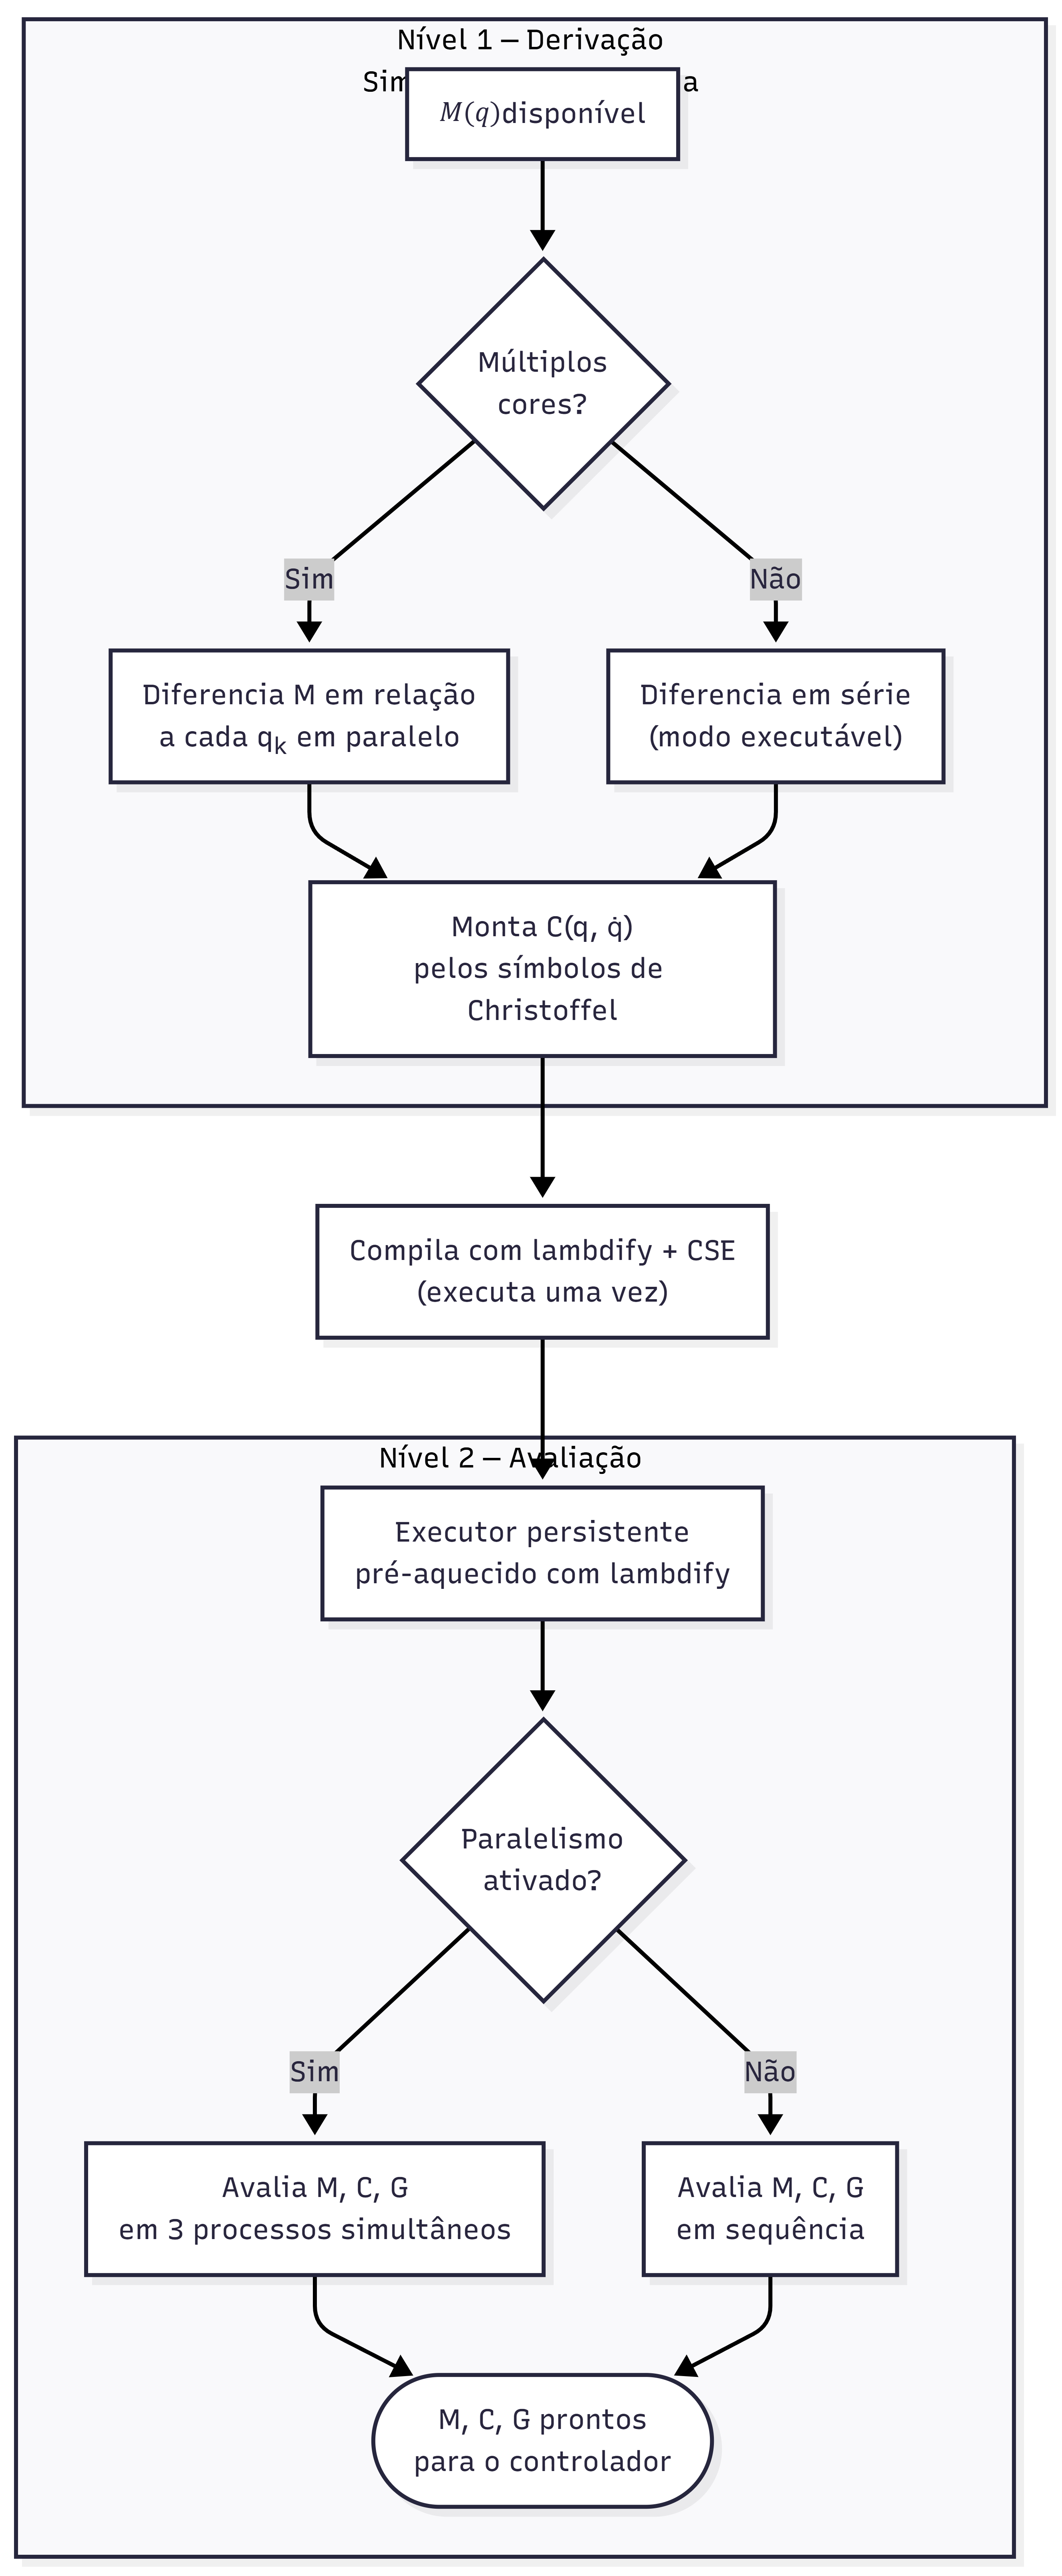
\includegraphics[width=0.5\textwidth]{figuras/Diagramas/Diagrama 12 — Paralelismo em Dois Níveis.png}
    \caption{Paralelismo em dois níveis no \textit{Hephaestus}: (Nível~1) derivação paralela de $\partial M/\partial q_k$ e das linhas de $C$ por \texttt{ProcessPoolExecutor} durante a geração \textit{offline} do modelo; (Nível~2) avaliação paralela e persistente de \texttt{func\_M}, \texttt{func\_C} e \texttt{func\_G} a cada passo de integração física durante a simulação \textit{online}.}
    \label{fig:paralelismo_2niveis}
\end{figure}

% ==============================================================================
\section{Considerações sobre a Complexidade Computacional}
\label{sec:complexidade}
% ==============================================================================

Resume-se, na Tabela~\ref{tab:complexidade}, a complexidade computacional das etapas de modelagem e simulação do \textit{Hephaestus}, comparada com as referências clássicas da literatura.

\begin{table}[h!]
\centering
\caption{Complexidade computacional das etapas de modelagem e simulação.}
\label{tab:complexidade}
\begin{tabular}{p{4.8cm} p{3.5cm} p{5.5cm}}
\hline
\textbf{Etapa} & \textbf{Complexidade} & \textbf{Referência / Observação} \\
\hline
Cinemática FK simbólica & $O(N^2)$ & Produto acumulado de matrizes $4\times4$ \cite{craig1989introduction} \\
Derivação de $M(q)$ (simbólica) & $O(N^3)$ & Jacobianos por elo \cite{siciliano2009robotics} \\
Derivação de $\partial M/\partial q_k$ & $O(N^4)$ (ingênuo) & Paralelizável por $N$ processos \cite{hollerbach1980recursive} \\
Cálculo de $C$ (Christoffel) & $O(N^3)$ simbólico & $N(N+1)/2$ pares por linha, $N$ linhas \cite{spong2020robot} \\
Compilação (\texttt{lambdify} + CSE) & $O(S)$, $S=$ tamanho expr. & Custo único; CSE reduz $S$ em 60--90\% \cite{alfred2007compilers, meurer2017sympy} \\
Avaliação numérica por passo & $O(N^2)$ & Mult. matriz-vetor $M\backslash(tau - C - G)$ \cite{golub2013matrix} \\
\hline
\end{tabular}
\end{table}

A comparação direta com o algoritmo de Newton-Euler recursivo, cuja complexidade é $O(N)$ tanto na geração quanto na avaliação \cite{luh1980online, hollerbach1980recursive}, evidencia o \textit{trade-off} fundamental da abordagem simbólica: maior custo de derivação (amortizado na fase \textit{offline}), em troca de equações explícitas que viabilizam análise, controle baseado em modelo e transparência pedagógica. Esse \textit{trade-off} é deliberado e justificado pelo objetivo do \textit{Hephaestus} como plataforma didática e de desenvolvimento de controladores \cite{corke2021toolbox}.

% ==============================================================================
\section{Síntese do Capítulo}
% ==============================================================================

Este capítulo descreveu em detalhe o processo completo de modelagem matemática simbólica implementado no \textit{Hephaestus}. A partir de uma especificação compacta da cadeia cinemática (\texttt{joint\_config} e \texttt{link\_vectors\_mask}), a \textit{engine} deriva automaticamente as expressões fechadas de $M(q)$, $C(q,\dot{q})$, $G(q)$ e $J(q)$ pelo formalismo de Euler-Lagrange via Jacobianos, com extensão para o cenário hidrodinâmico por herança da classe \texttt{RobotMathHydro}. A geração simbólica é acelerada por paralelismo de processos na derivação de Christoffel, e as expressões resultantes são compiladas para funções NumPy de alto desempenho por \texttt{lambdify} com CSE, eliminando o gargalo de avaliação simbólica em tempo de simulação. O executor persistente completa a cadeia de otimização, permitindo avaliação paralela de $M$, $C$ e $G$ a cada passo de integração sem custo de \textit{respawn} de processos.

A arquitetura resultante é matematicamente transparente , cada equação pode ser inspecionada simbolicamente , e computacionalmente eficiente , capaz de simular manipuladores de até 8 GDL em tempo real no \textit{hardware} alvo. O Capítulo seguinte descreve a camada de simulação numérica que consome as equações aqui derivadas, detalhando o integrador simplético, os controladores implementados e o planejamento de trajetórias.

  \chapter{Simulação Numérica e Planejamento de Trajetórias}
\label{cap:simulacao}

Este capítulo descreve a camada de simulação numérica do \textit{Hephaestus}, implementada na classe \texttt{RobotSimulator} do módulo \texttt{simulator.py}. Enquanto o Capítulo~\ref{cap:modelagem} tratou da derivação simbólica e da compilação das equações de movimento, este capítulo aborda como essas equações são integradas numericamente em malha fechada para rastrear trajetórias cartesianas com controle dinâmico de alta fidelidade. As contribuições técnicas centrais deste capítulo compreendem: o planejamento de trajetórias com polinômio cúbico no espaço cartesiano (segmentos lineares e arcos circulares); a extensão do algoritmo CLIK para controle de orientação no espaço de tarefa 6D; a inicialização robusta de postura por Levenberg-Marquardt com busca em linha; o integrador simplético com \textit{substeps} independentes; quatro estratégias de controle não-linear comparáveis em uma única interface; e modelos de forças dissipativas para atrito nas juntas e arrasto hidrodinâmico.

% ==============================================================================
\section{Arquitetura do Simulador}
\label{sec:arq_simulador}
% ==============================================================================

A classe \texttt{RobotSimulator} recebe como entrada um objeto \texttt{RobotMathEngine} (ou \texttt{RobotMathHydro}) previamente processado e realiza, em seu construtor, a compilação de todas as expressões simbólicas em funções numéricas. Conforme descrito na Seção~\ref{sec:lambdify_cse} do Capítulo~\ref{cap:modelagem}, essa compilação é realizada por \texttt{sp.lambdify()} com CSE ativo, produzindo as funções \texttt{func\_M}, \texttt{func\_C}, \texttt{func\_G}, \texttt{func\_J} e o vetor \texttt{funcs\_fk\_all\_links}, que avalia a posição cartesiana de cada elo para a visualização animada \cite{meurer2017sympy}.

A interface pública principal é o método \texttt{run()}, cuja assinatura unifica os parâmetros de configuração da trajetória, do controlador, do integrador e das forças dissipativas em um único ponto de entrada. Internamente, o método \texttt{run()} organiza a simulação em quatro fases:

\begin{enumerate}
    \item \textbf{Inicialização da Postura}: a posição cartesiana inicial $P_i$ é passada ao Levenberg-Marquardt (\texttt{solve\_ik\_initial}) para convergir a uma configuração de juntas $q_0$ compatível antes do início da trajetória.
    \item \textbf{Loop de Integração}: a cada passo visual $\Delta t_{\text{vis}}$, são executados $N_s$ \textit{substeps} físicos $\Delta t_{\text{phys}} = \Delta t_{\text{vis}} / N_s$, cada um compreendendo: planejamento de trajetória, CLIK, avaliação de $M$, $C$, $G$, cálculo do torque de controle, aplicação das forças dissipativas e integração simplética.
    \item \textbf{Coleta de Resultados}: ao final de cada passo visual, os erros de junta $e = q_d - q$, os torques aplicados $\tau$ e os dados de animação (posições FK de todos os elos e matrizes de rotação) são armazenados.
    \item \textbf{Retorno}: o método retorna as séries temporais $\{t_i, e_i, \tau_i\}$ e a lista de frames de animação, que são consumidos pela interface gráfica para plotagem e renderização interativa.
\end{enumerate}

A detecção automática da fronteira veículo/braço — pela contagem das juntas iniciais sem vetor de elo estrutural nulo — permite que o simulador opere tanto em manipuladores terrestres puros quanto em UVMSs, compilando separadamente a matriz de rotação do frame do veículo (\texttt{func\_R\_vehicle}) para visualização da orientação do corpo base \cite{antonelli2014modelling, fossen2011handbook}. As Figuras~\ref{fig:loop_init} e~\ref{fig:loop_controle} detalham o fluxo interno do método \texttt{run()}: a fase de inicialização (Figura~\ref{fig:loop_init}) e o passo de controle repetido a cada substep físico (Figura~\ref{fig:loop_controle}).

\begin{figure}[htbp]
    \centering
    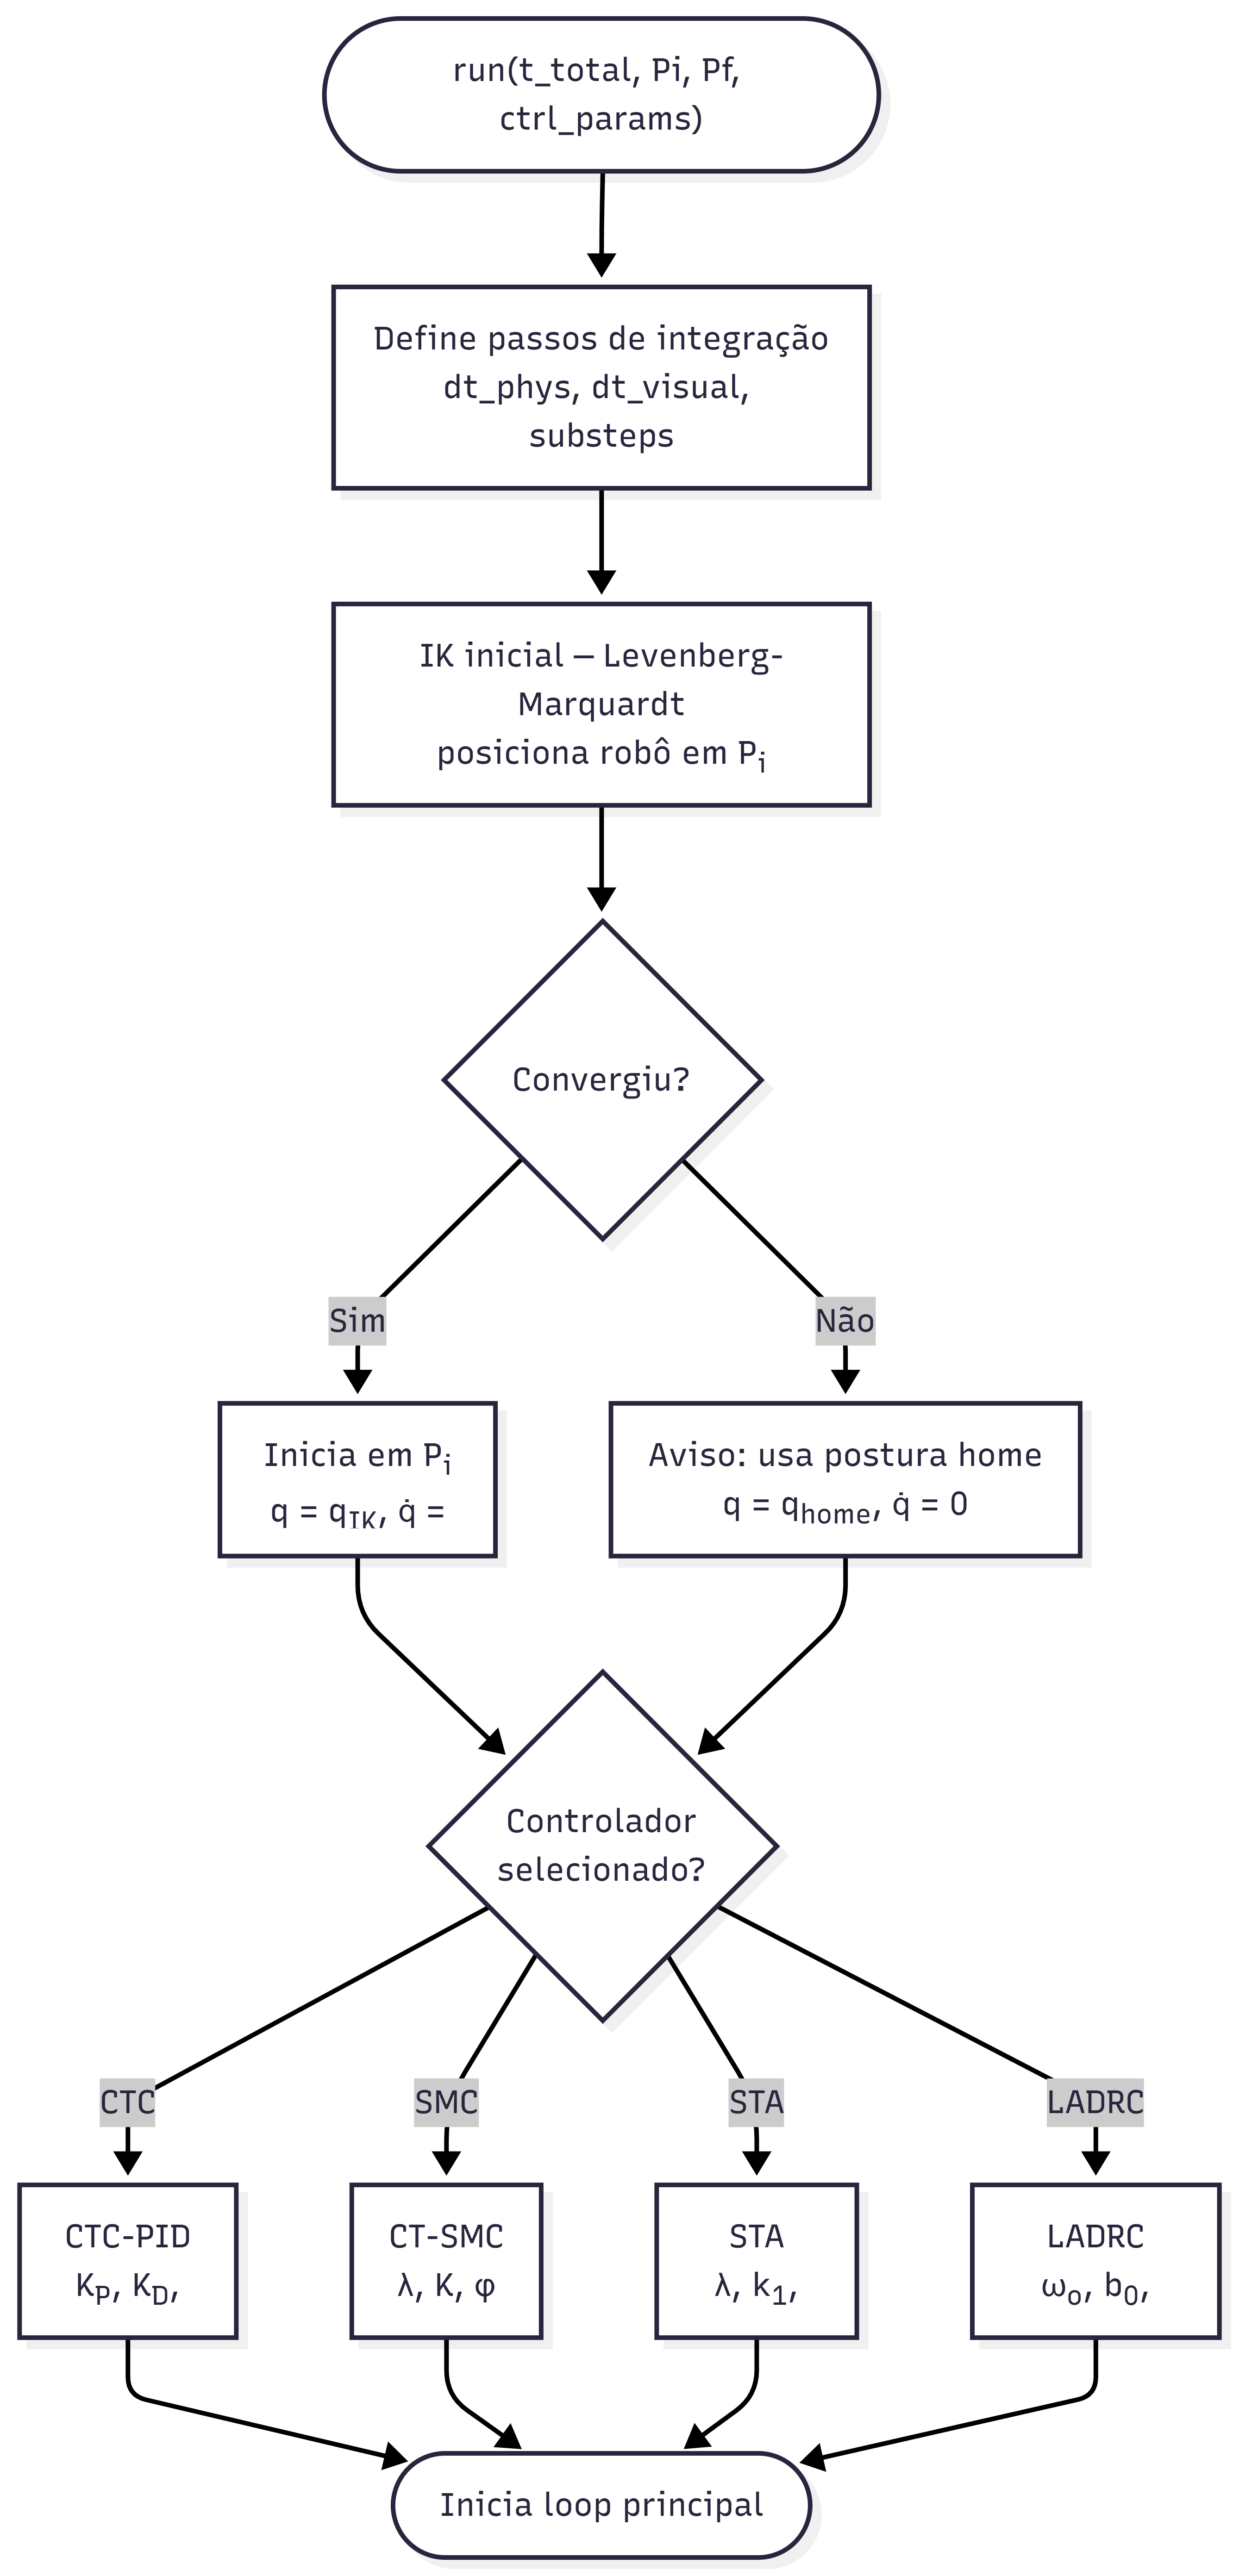
\includegraphics[width=0.65\textwidth]{figuras/Diagramas/Diagrama 7a — Loop de Simulação Inicialização.png}
    \caption{Fase de inicialização do simulador: resolução da IK estática por Levenberg-Marquardt com busca em linha (Seção~\ref{sec:ik_initial}), configuração do controlador e do executor paralelo, e verificação das condições de estabilidade numérica (Seção~\ref{sec:estabilidade_num}).}
    \label{fig:loop_init}
\end{figure}

\begin{figure}[htbp]
    \centering
    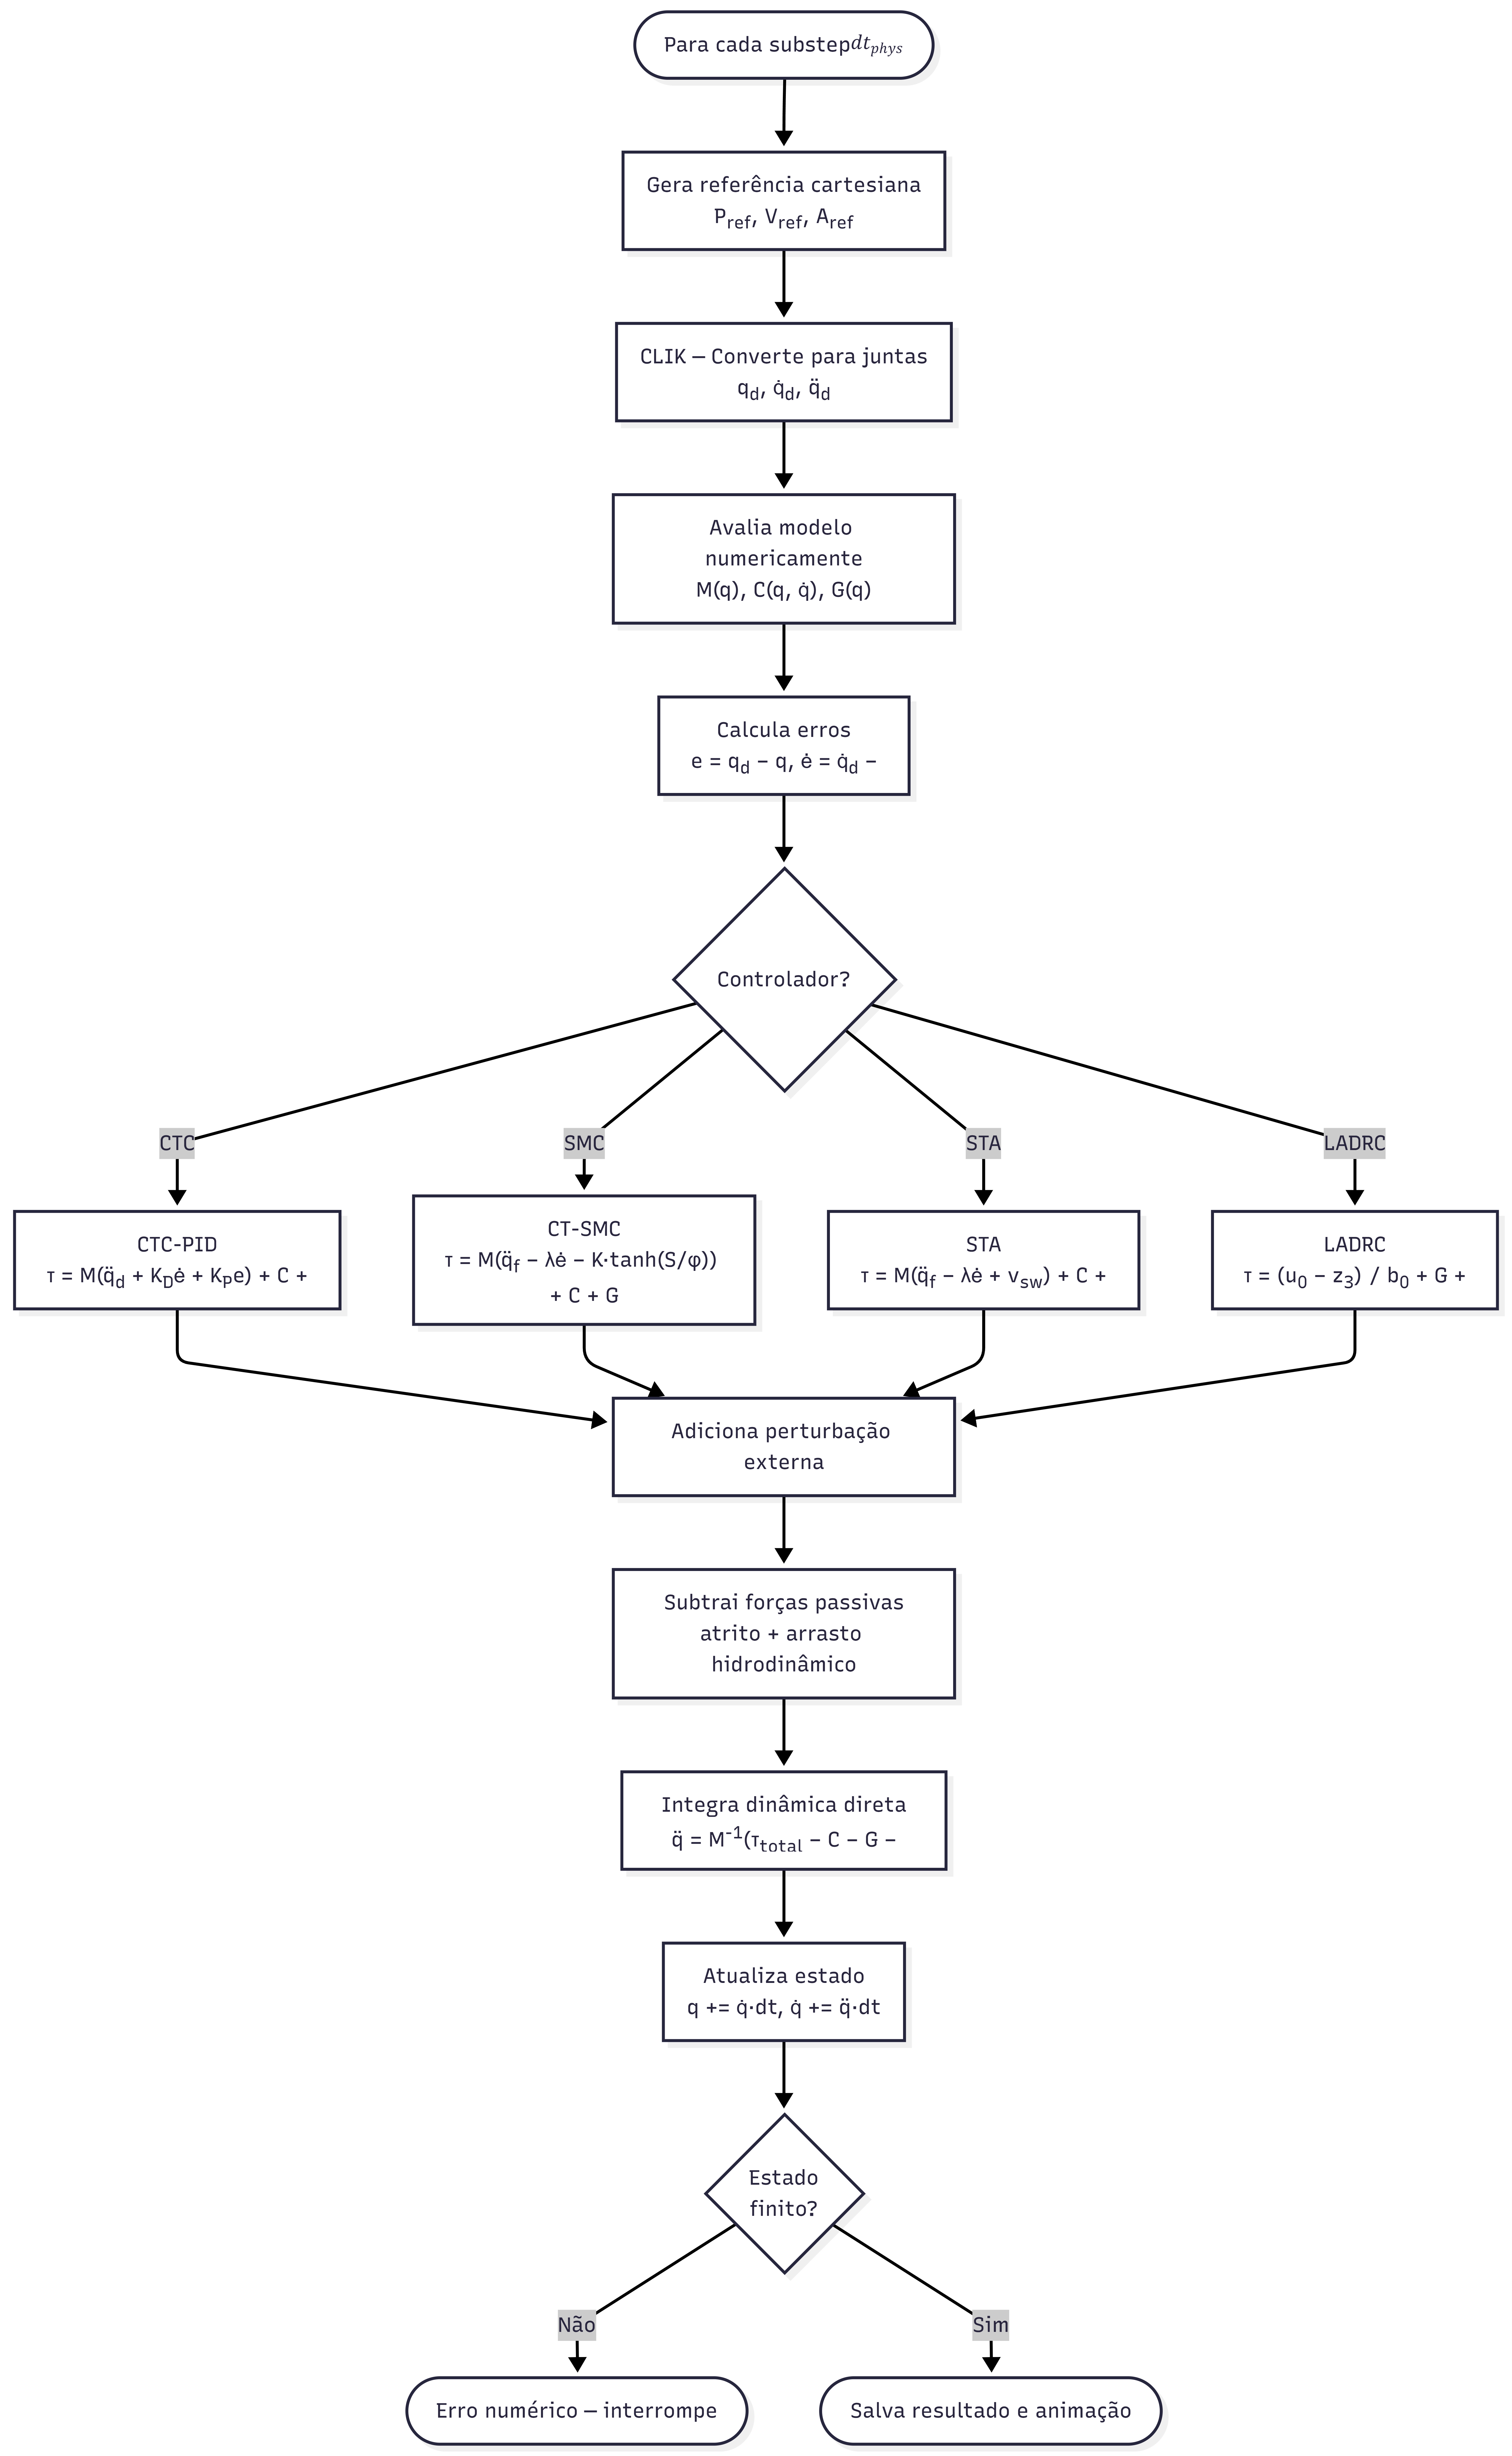
\includegraphics[width=0.88\textwidth]{figuras/Diagramas/Diagrama 7b — Loop de Simulação Passo de Controle.png}
    \caption{Passo de controle físico executado a cada substep $\Delta t_{\text{phys}}$: planejamento de trajetória, CLIK 6D, avaliação paralela de $M$, $C$, $G$, cálculo do torque de controle, aplicação das forças dissipativas e integração simplética de Euler (Equações~\eqref{eq:symplectic1}--\eqref{eq:symplectic2}).}
    \label{fig:loop_controle}
\end{figure}

% ==============================================================================
\section{Planejamento de Trajetórias no Espaço Cartesiano}
\label{sec:traj_planning}
% ==============================================================================

O planejamento de trajetórias define as referências de posição $P_{\text{ref}}(t)$, velocidade $\dot{P}_{\text{ref}}(t)$ e aceleração $\ddot{P}_{\text{ref}}(t)$ que o efetuador deve rastrear ao longo do tempo. Siciliano et al. \cite{siciliano2009robotics} e Craig \cite{craig1989introduction} distinguem o planejamento no espaço de juntas do planejamento no espaço cartesiano; este trabalho adota o segundo, em que as referências são geradas diretamente na posição do efetuador e convertidas para comandos de junta pelo CLIK a cada instante.

\subsection{Polinômio Cúbico de Interpolação}

Toda trajetória implementada no \textit{Hephaestus} utiliza o parâmetro de tempo normalizado $\tau = t / T \in [0,1]$, onde $T$ é a duração total do segmento, interpolado pelo polinômio cúbico:
\begin{equation}
    s(\tau) = 3\tau^2 - 2\tau^3,
    \label{eq:cubic_s}
\end{equation}
com derivadas:
\begin{equation}
    \dot{s} = \frac{6\tau - 6\tau^2}{T}, \qquad
    \ddot{s} = \frac{6 - 12\tau}{T^2}.
    \label{eq:cubic_ds}
\end{equation}

Este perfil garante $s(0) = 0$, $s(1) = 1$, $\dot{s}(0) = \dot{s}(1) = 0$ — ou seja, partida e parada suaves — e aceleração máxima $|\ddot{s}|_{\max} = 6/T^2$ no instante $T/2$ \cite{siciliano2009robotics}. A continuidade da velocidade nos extremos é essencial para evitar descontinuidades no sinal de referência do CLIK que seriam amplificadas pelos ganhos derivativos do controlador \cite{craig1989introduction}. O polinômio de grau 5 (que garantiria continuidade de aceleração nos extremos) não foi adotado por apresentar pico de aceleração levemente superior para o mesmo tempo de trajetória, conforme análise comparativa de Siciliano et al. \cite{siciliano2009robotics}.

\subsection{Segmento de Reta}

Para a trajetória linear de $P_i$ a $P_f$, a referência cartesiana é:
\begin{align}
    P_{\text{ref}}(t) &= P_i + (P_f - P_i)\,s(\tau), \label{eq:traj_line_P}\\
    \dot{P}_{\text{ref}}(t) &= (P_f - P_i)\,\dot{s}(\tau), \label{eq:traj_line_V}\\
    \ddot{P}_{\text{ref}}(t) &= (P_f - P_i)\,\ddot{s}(\tau). \label{eq:traj_line_A}
\end{align}

A disponibilidade explícita de $\dot{P}_{\text{ref}}$ e $\ddot{P}_{\text{ref}}$ é fundamental para o \textit{feedforward} de velocidade e aceleração no CLIK, que reduz o erro de rastreamento em regime dinâmico em comparação com o uso exclusivo de realimentação proporcional de posição \cite{chiaverini1994review, siciliano2009robotics}.

\subsection{Arco Circular}

A trajetória circular é parametrizada pelo centro $C$, dois vetores ortonormais $e_1$, $e_2$ no plano do arco, raio $R$, ângulo inicial $\theta_0$ e ângulo final $\theta_f$. O centro é determinado geometricamente como o ponto equidistante de $P_i$ e $P_f$ ao longo da direção perpendicular à corda $v = P_f - P_i$ no plano definido pelo vetor normal $\hat{n}$:
\begin{equation}
    C = \frac{P_i + P_f}{2} \pm h\,\frac{(P_f - P_i) \times \hat{n}}{\|(P_f - P_i) \times \hat{n}\|}, \qquad
    h = \sqrt{R^2 - \frac{\|P_f - P_i\|^2}{4}},
    \label{eq:circle_center}
\end{equation}
com sinal determinado pelo parâmetro de sentido de percurso. A trajetória é então:
\begin{equation}
    P(t) = C + R\left[\cos(\theta(t))\,e_1 + \sin(\theta(t))\,e_2\right], \quad
    \theta(t) = \theta_0 + (\theta_f - \theta_0)\,s(\tau),
    \label{eq:circle_traj}
\end{equation}
com velocidade e aceleração obtidas por diferenciação analítica:
\begin{align}
    \dot{P}(t) &= R\,\dot{\theta}\,\left[-\sin(\theta)\,e_1 + \cos(\theta)\,e_2\right], \label{eq:circle_V}\\
    \ddot{P}(t) &= R\,\left[\ddot{\theta}\,\hat{t}(\theta) + \dot{\theta}^2\,\hat{n}(\theta)\right],
    \label{eq:circle_A}
\end{align}
onde $\hat{t} = -\sin(\theta)\,e_1 + \cos(\theta)\,e_2$ é o vetor tangente e $\hat{n} = -\cos(\theta)\,e_1 - \sin(\theta)\,e_2$ é o vetor normal centrípeto. A componente centrípeta $\dot{\theta}^2\,\hat{n}$ da aceleração é frequentemente omitida em abordagens simplificadas, mas sua inclusão é necessária para que o \textit{feedforward} de aceleração no CLIK seja fisicamente correto em trajetórias circulares de alta velocidade \cite{siciliano2009robotics}.

Uma verificação de segurança automática é aplicada: se a distância entre $P_i$ e $P_f$ excede o diâmetro $2R$, o raio é automaticamente estendido para $R = \|P_f - P_i\|/2 + \varepsilon$, garantindo geometria factível. Caso o vetor $(P_f - P_i) \times \hat{n}$ seja nulo (pontos colineares com a normal), a trajetória degrada graciosamente para um segmento de reta \cite{siciliano2009robotics}. A Figura~\ref{fig:traj_planning} apresenta o fluxo de geração das referências de posição, velocidade e aceleração para os dois tipos de trajetória implementados e a integração com o polinômio cúbico.

\begin{figure}[htbp]
    \centering
    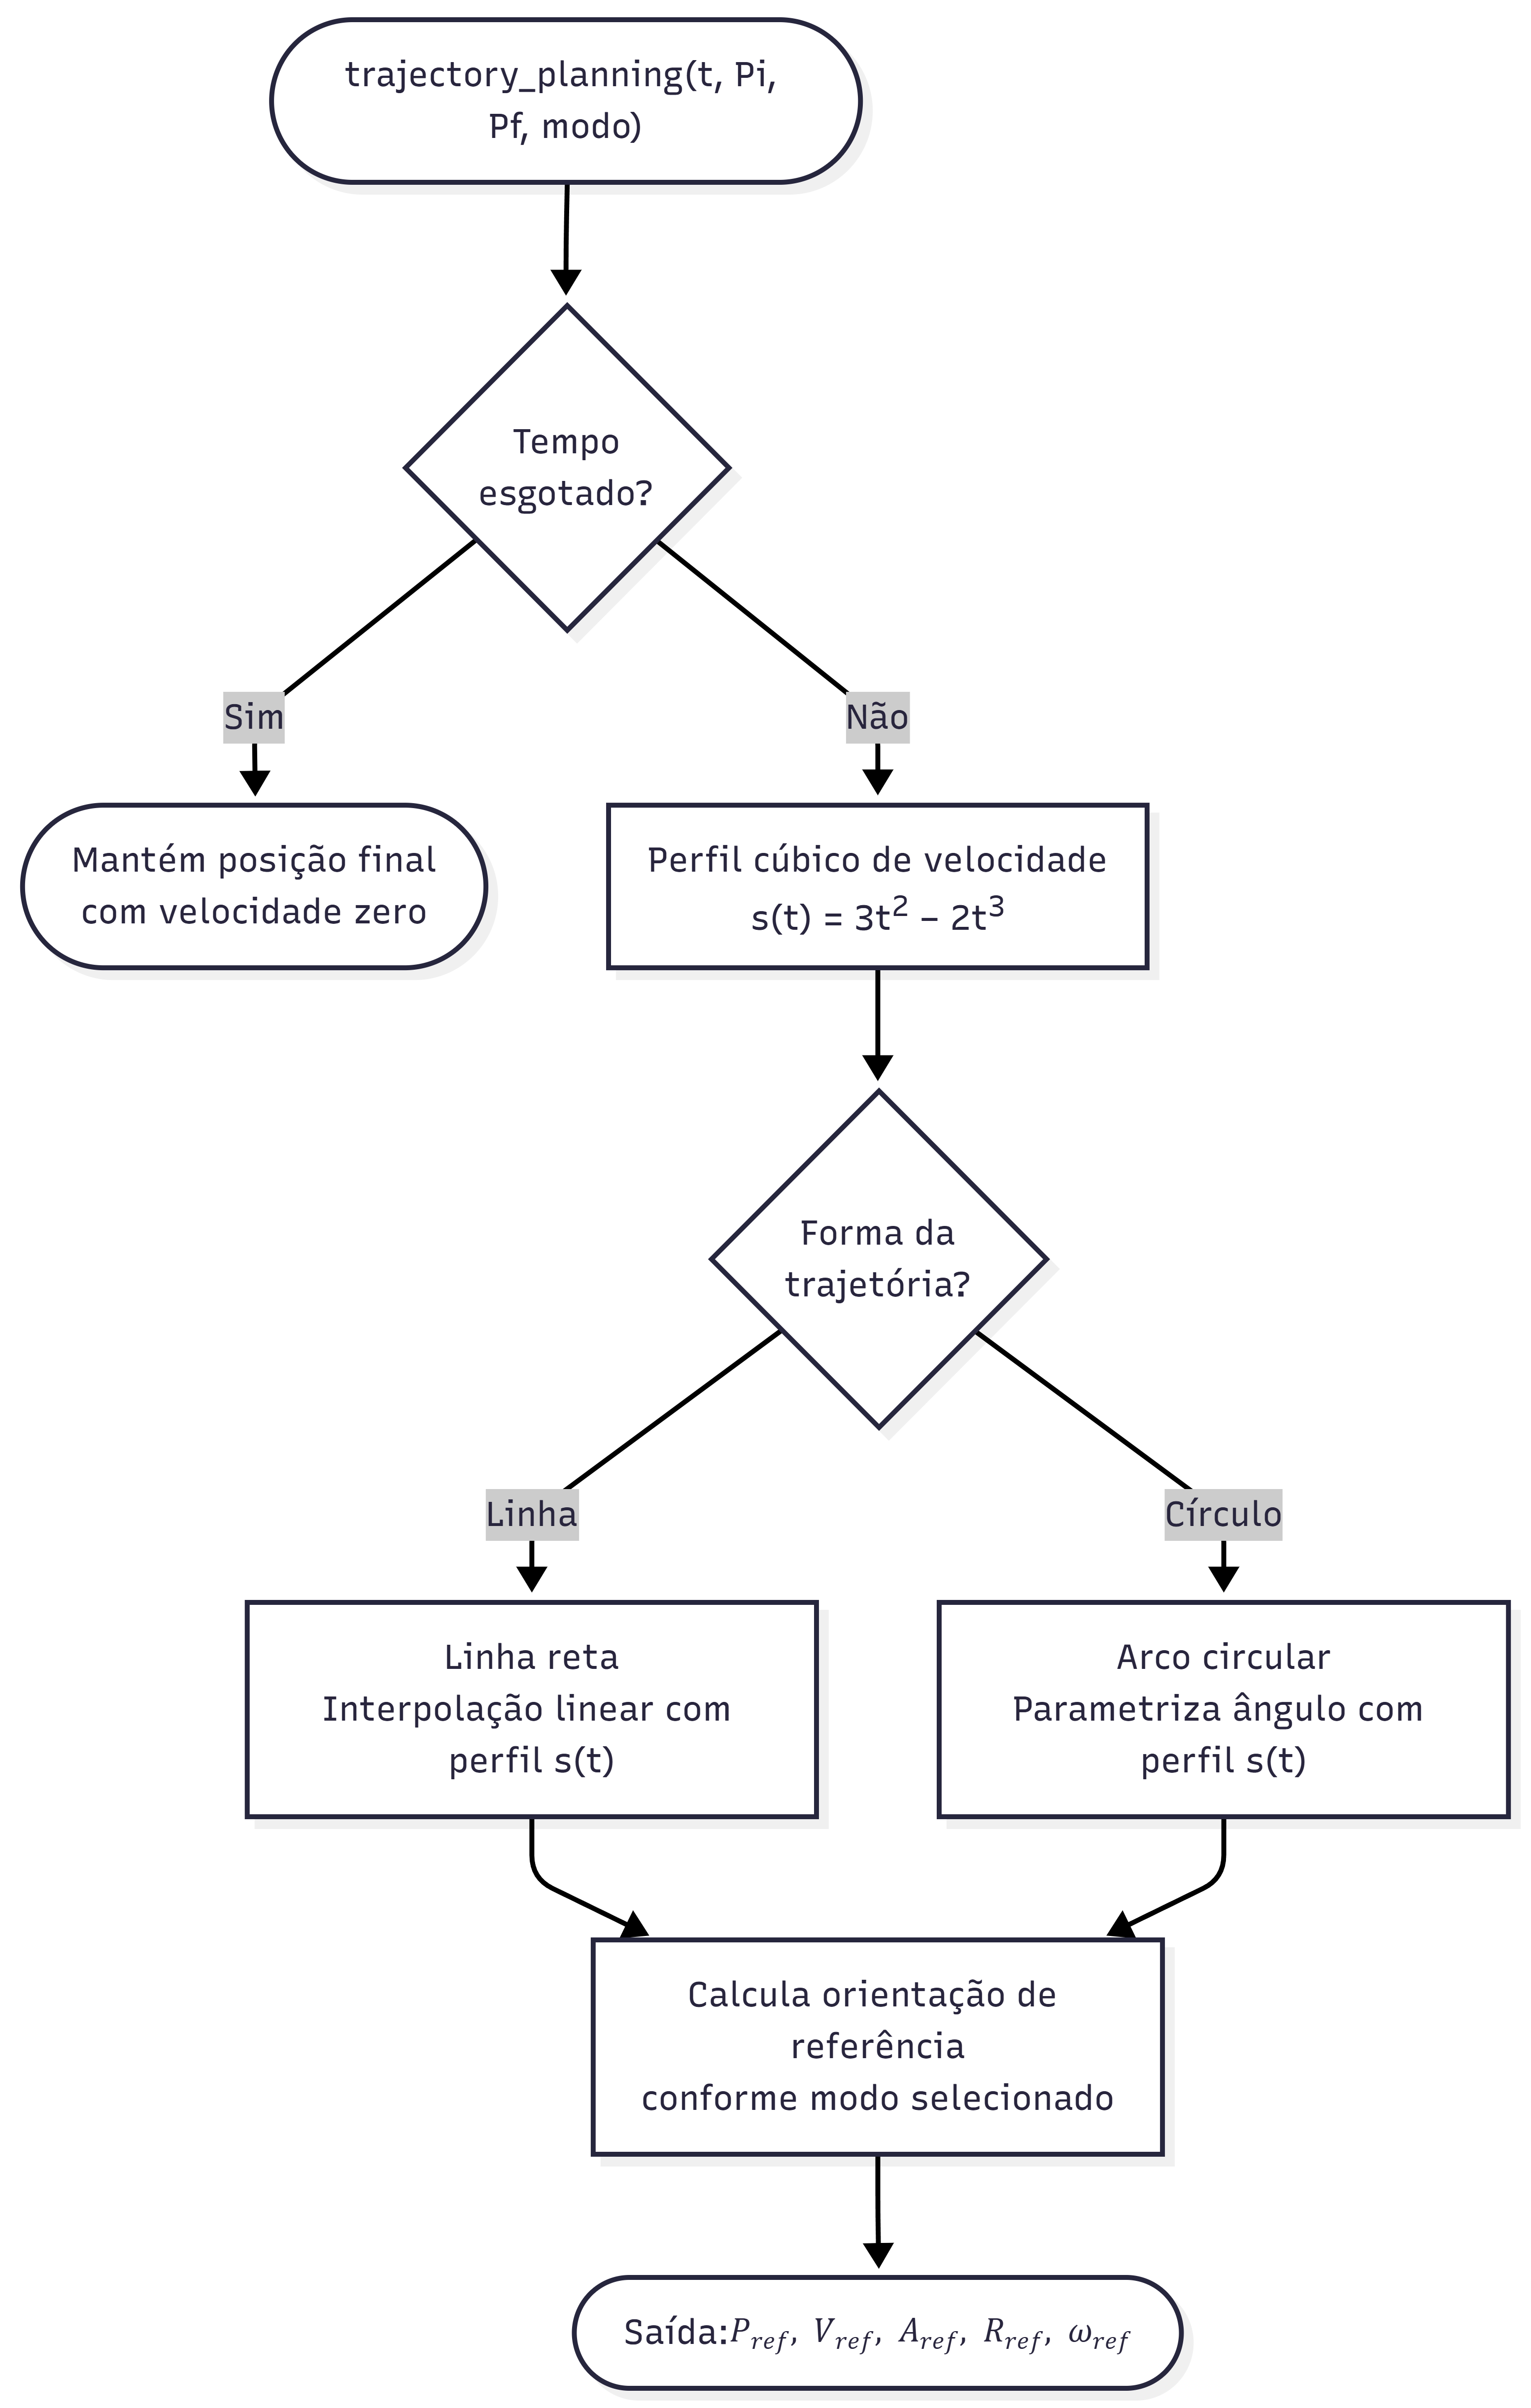
\includegraphics[width=0.90\textwidth]{figuras/Diagramas/Diagrama 5 — Planejamento de Trajetória.png}
    \caption{Fluxo de planejamento de trajetória no espaço cartesiano: o parâmetro cúbico $s(\tau)$ (Equação~\eqref{eq:cubic_s}) é aplicado ao segmento de reta (Equações~\eqref{eq:traj_line_P}--\eqref{eq:traj_line_A}) ou ao arco circular (Equações~\eqref{eq:circle_traj}--\eqref{eq:circle_A}), gerando triplas $\{P_{\text{ref}}, \dot{P}_{\text{ref}}, \ddot{P}_{\text{ref}}\}$ a cada passo de integração para o CLIK \cite{siciliano2009robotics, craig1989introduction}.}
    \label{fig:traj_planning}
\end{figure}

\subsection{Modos de Referência de Orientação}
\label{sec:orient_modes}

O \textit{Hephaestus} suporta seis modos distintos de referência de orientação do efetuador, selecionáveis independentemente do tipo de trajetória posicional:

\begin{enumerate}
    \item \textbf{Livre} (\textit{orientation-free}): nenhuma restrição de orientação é imposta; o CLIK opera apenas com o Jacobiano posicional $3 \times N$. Este modo é o padrão e adequado para tarefas de posicionamento puro.
    
    \item \textbf{Fixa}: a orientação é mantida constante e igual à rotação $R_0$ capturada na postura inicial. Implementado como $R_{\text{ref}}(t) = R_0$, $\omega_{\text{ref}} = 0$. Útil para tarefas de transporte com efetuador estabilizado \cite{siciliano2009robotics}.
    
    \item \textbf{Tangente à Trajetória}: o eixo $z$ do efetuador é alinhado à tangente instantânea da trajetória:
    \begin{equation}
        \hat{z}(t) = \frac{\dot{P}_{\text{ref}}(t)}{\|\dot{P}_{\text{ref}}(t)\|}, \qquad
        \omega_{\text{ref}} = \hat{z} \times \dot{\hat{z}},
        \label{eq:orient_tangent}
    \end{equation}
    onde $\dot{\hat{z}}$ é obtido por diferenciação analítica de $\hat{z}$ em relação ao tempo. Empregado em tarefas de corte, pintura ou inspeção ao longo da trajetória \cite{siciliano2009robotics}.
    
    \item \textbf{Apontar para o Alvo}: o eixo $z$ do efetuador é continuamente orientado em direção ao ponto $P_f$:
    \begin{equation}
        \hat{z}(t) = \frac{P_f - P_{\text{ref}}(t)}{\|P_f - P_{\text{ref}}(t)\|}, \qquad
        \omega_{\text{ref}} = \hat{z} \times \left[\frac{-\dot{P}_{\text{ref}}}{\|P_f - P_{\text{ref}}\|} - \frac{(P_f - P_{\text{ref}}) \cdot (-\dot{P}_{\text{ref}})}{\|P_f - P_{\text{ref}}\|^3}(P_f - P_{\text{ref}})\right].
        \label{eq:orient_point}
    \end{equation}
    Adequado para tarefas de solda, furação ou interação com um alvo fixo \cite{chiaverini1997singularity}.
    
    \item \textbf{SLERP} (\textit{Spherical Linear Interpolation}): interpola suavemente a orientação entre $R_0$ (postura inicial) e $R_f$ (orientação final desejada) ao longo do geodésico em $SO(3)$:
    \begin{equation}
        R_{\text{ref}}(t) = R_0 \left(R_0^\top R_f\right)^{s(\tau)}, \qquad
        \omega_{\text{ref}} = \dot{s}\,\theta_{\text{total}}\,R_0\,\hat{a}_{\text{local}},
        \label{eq:slerp_impl}
    \end{equation}
    onde $\theta_{\text{total}}$ é o ângulo total de rotação e $\hat{a}_{\text{local}}$ é o eixo de rotação no referencial de $R_0$, extraído pela decomposição eixo-ângulo de $R_0^\top R_f$ \cite{shoemake1985animating, dam1998quaternions}. A velocidade angular de referência $\omega_{\text{ref}}$ garante que o \textit{feedforward} rotacional seja fisicamente correto, não apenas proporcional ao erro.
    
    \item \textbf{Normal à Superfície}: o eixo $z$ é mantido alinhado a um vetor normal fixo $\hat{n}$ fornecido pelo usuário, com $\omega_{\text{ref}} = 0$. Adequado para tarefas de usinagem ou inspeção perpendicular a superfícies planas \cite{siciliano2009robotics}.
\end{enumerate}

Os modos 2 a 6 ativam o Jacobiano completo $6 \times N$ no CLIK, descrito na Seção~\ref{sec:clik_6d}, combinando controle de posição e orientação no mesmo algoritmo. A Figura~\ref{fig:modos_orientacao} compara os seis modos de referência de orientação implementados, indicando o sinal de referência gerado por cada um e os casos de uso típicos.

\begin{figure}[htbp]
    \centering
    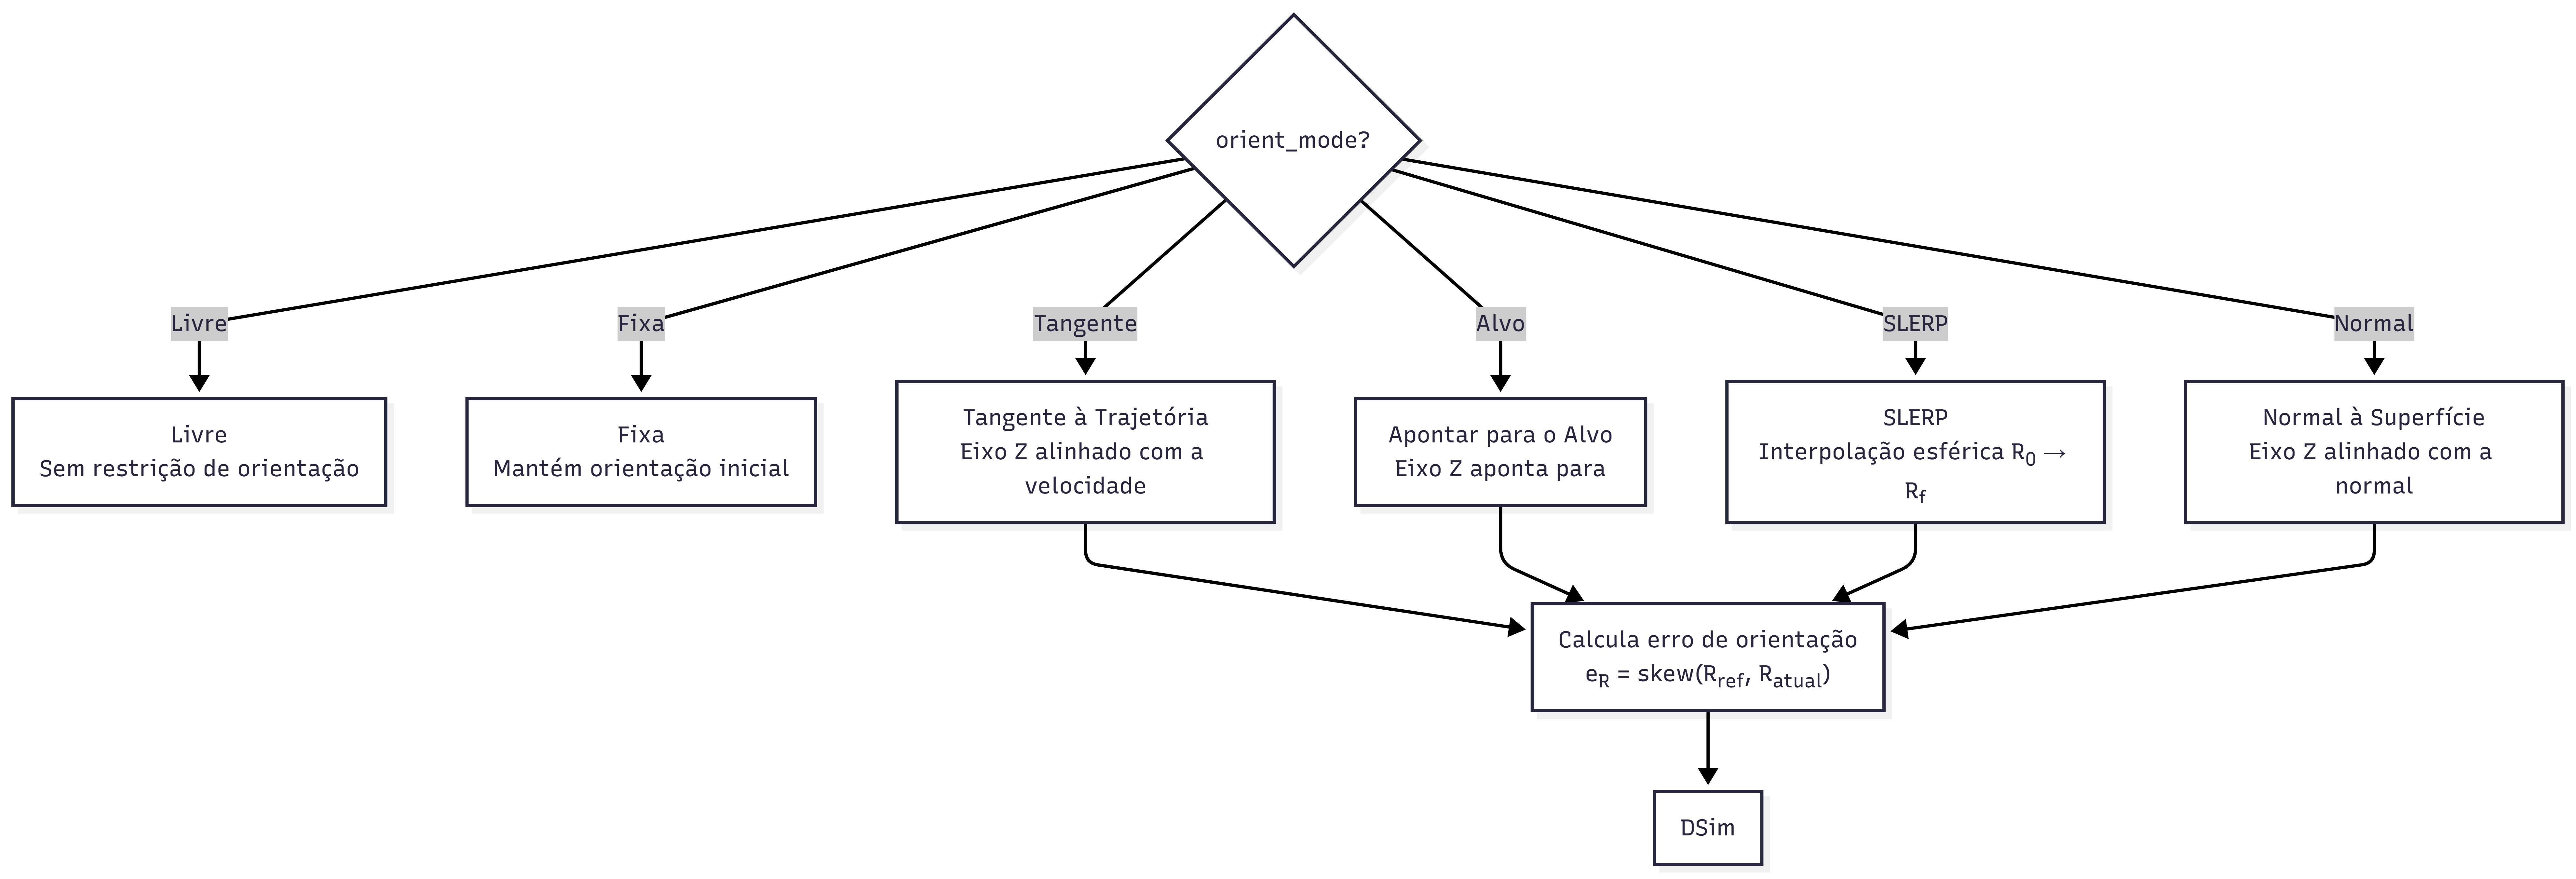
\includegraphics[width=0.9\textwidth]{figuras/Diagramas/Diagrama 6b — Modos de Orientação do Efetuador.png}
    \caption{Modos de referência de orientação do efetuador disponíveis no \textit{Hephaestus}: Livre (apenas controle posicional), Fixa, Tangente à Trajetória, Apontar para o Alvo, SLERP geodésico \cite{shoemake1985animating} e Normal à Superfície. Os modos 2--6 ativam o Jacobiano completo $J \in \mathbb{R}^{6 \times N}$ e o erro de orientação da Equação~\eqref{eq:orient_error_impl}.}
    \label{fig:modos_orientacao}
\end{figure}

% ==============================================================================
\section{Inicialização da Postura: Levenberg-Marquardt com Busca em Linha}
\label{sec:ik_initial}
% ==============================================================================

Antes do início da trajetória, o \textit{Hephaestus} resolve o problema de IK estática para posicionar o efetuador em $P_i$ a partir da postura inicial $q_0$ (postura \textit{home} ou última postura convergida). Para garantir convergência robusta mesmo próximo de singularidades ou partindo de configurações distantes, é empregada uma variante do algoritmo de Levenberg-Marquardt \cite{marquardt1963algorithm, more2006levenberg} com busca em linha por \textit{backtracking} (regra de Armijo \cite{armijo1966minimization}).

O algoritmo iterativo é descrito a seguir. A cada iteração $k$:
\begin{enumerate}
    \item Avalia a posição atual $p_k = f_{\text{FK}}(q_k)$ e o erro $e_k = P_i - p_k$.
    \item Se $\|e_k\| < \varepsilon_{\text{tol}}$, termina com convergência.
    \item Calcula o passo DLS:
    \begin{equation}
        \Delta q = J_{\text{pos}}^\top \left(J_{\text{pos}} J_{\text{pos}}^\top + \lambda_k^2 I_3\right)^{-1} e_k,
        \label{eq:lm_step}
    \end{equation}
    onde $J_{\text{pos}} \in \mathbb{R}^{3 \times N}$ é o Jacobiano posicional e $\lambda_k$ é o parâmetro de amortecimento corrente.
    \item Executa busca em linha por \textit{backtracking}: tenta $q_{k+1} = q_k + \alpha \Delta q$ com $\alpha = 1, 0.5, 0.25, \ldots$ até $\|P_i - f_{\text{FK}}(q_{k+1})\| < \|e_k\|$.
    \item Atualiza $\lambda$ adaptativamente: $\lambda \leftarrow 0.9\lambda$ se houve descida (passo aceito), $\lambda \leftarrow 1.5\lambda$ se não houve (passo rejeitado), com limites $\lambda \in [10^{-4},\, 10]$.
    \item Detecta estagnação: se $|\|e_{k-1}\| - \|e_k\|| < 0.1\,\varepsilon_{\text{tol}}$ por 10 iterações consecutivas, interrompe.
\end{enumerate}

A estratégia adaptativa de $\lambda$ é a essência do algoritmo de Levenberg-Marquardt: para erros grandes (longe do mínimo), $\lambda$ grande amortece o passo, comportando-se como o método do gradiente; próximo do mínimo, $\lambda$ pequeno permite convergência quadrática típica de Newton-Gauss \cite{more2006levenberg}. A combinação com a busca em linha de Armijo confere estabilidade adicional quando o Jacobiano é mal-condicionado, conforme demonstrado por Nakamura e Hanafusa \cite{nakamura1986inverse} e Wampler \cite{wampler2007manipulator} para IK de manipuladores com singularidades.

% ==============================================================================
\section{Cinemática Inversa em Malha Fechada (CLIK)}
\label{sec:clik}
% ==============================================================================

\subsection{Formulação do CLIK Posicional (3D)}

Durante a trajetória, a cada passo de integração, o CLIK (Closed-Loop Inverse Kinematics) \cite{samson1991robot, chiaverini1994review} converte a referência cartesiana $\{P_{\text{ref}}, \dot{P}_{\text{ref}}, \ddot{P}_{\text{ref}}\}$ em referências de junta $\{q_d, \dot{q}_d, \ddot{q}_d\}$. A lei de velocidade de junta no modo posicional é:
\begin{equation}
    \dot{q}_d = J_{\text{DLS}}^{\dagger}\left[\dot{P}_{\text{ref}} + K_P\,e_{\text{pos}}\right] + (I - J_{\text{DLS}}^{\dagger} J_{\text{pos}})\,\dot{q}_0,
    \label{eq:clik_pos}
\end{equation}
onde $e_{\text{pos}} = P_{\text{ref}} - p_{\text{curr}}$ é o erro de posição cartesiano, $K_P = K_{p,\text{IK}} \cdot I_3$ é o ganho proporcional do CLIK, e o último termo projeta uma velocidade auxiliar $\dot{q}_0$ no espaço nulo de $J_{\text{pos}}$ para controle de redundância \cite{chiaverini1997singularity, liegeois1977automatic}.

A pseudo-inversa amortecida (DLS) $J_{\text{DLS}}^{\dagger} \in \mathbb{R}^{N \times 3}$ é \cite{nakamura1986inverse, wampler2007manipulator}:
\begin{equation}
    J_{\text{DLS}}^{\dagger} = J_{\text{pos}}^\top \left(J_{\text{pos}} J_{\text{pos}}^\top + \lambda_{\text{DLS}}^2 I_3\right)^{-1}.
    \label{eq:dls_pos}
\end{equation}

A posição de junta de referência é obtida por integração de Euler explícita:
\begin{equation}
    q_d(t + \Delta t) = q_{\text{curr}} + \dot{q}_d\, \Delta t,
    \label{eq:clik_q_int}
\end{equation}
e o termo de aceleração de referência é calculado para \textit{feedforward}:
\begin{equation}
    \ddot{q}_d = J_{\text{DLS}}^{\dagger} \left[\ddot{P}_{\text{ref}} + K_D^{\text{IK}}\,\dot{e}_{\text{vel}} - \dot{J}\dot{q}\right],
    \label{eq:clik_ddq}
\end{equation}
onde $K_D^{\text{IK}} = 2\sqrt{K_P}$ e o termo $\dot{J}\dot{q}$ é a correção de deriva do Jacobiano, calculada por diferença finita de $J_{\text{pos}}$ entre passos consecutivos \cite{siciliano2009robotics}.

\subsection{Limitação de Velocidade de Junta}

Para evitar descontinuidades e prevenir movimentos bruscos próximos de singularidades, a velocidade de junta total $\dot{q}_d$ (incluindo a contribuição do espaço nulo) é saturada suavemente pela função hiperbólica tangente:
\begin{equation}
    \dot{q}_d^{\text{sat}} = \dot{q}_{\text{lim}}\,\tanh\!\left(\frac{\dot{q}_d}{\dot{q}_{\text{lim}}}\right),
    \label{eq:dq_saturation}
\end{equation}
onde $\dot{q}_{\text{lim}}$ é o limite de velocidade por junta. O uso de $\tanh$ em vez de \textit{clipping} linear garante diferenciabilidade e preserva a direção do vetor de velocidade para valores abaixo do limite, o que é importante para a qualidade do \textit{feedforward} \cite{siciliano2009robotics}.

\subsection{Controle de Orientação no Espaço de Tarefa 6D}
\label{sec:clik_6d}

Quando um modo de orientação diferente de \textit{Livre} é selecionado, o CLIK é estendido para o espaço de tarefa 6D, utilizando o Jacobiano completo $J \in \mathbb{R}^{6 \times N}$ e combinando o controle de posição e orientação em uma única lei de velocidade. O erro de orientação é calculado pela formulação de anel (skew-symmetric) \cite{chiaverini1997singularity}:
\begin{equation}
    e_R = \frac{1}{2}\,\text{vee}\!\left(R_{\text{ref}} R_{\text{curr}}^\top - R_{\text{curr}} R_{\text{ref}}^\top\right),
    \label{eq:orient_error_impl}
\end{equation}
onde $R_{\text{curr}}$ é a rotação corrente do efetuador obtida por $\texttt{func\_R\_last}(q, \cdot)$ e $R_{\text{ref}}$ é a rotação de referência do modo selecionado (Seção~\ref{sec:orient_modes}). Esta formulação é proporcional ao vetor eixo-ângulo para erros pequenos e evita singularidades de representação por ângulos de Euler \cite{siciliano2009robotics}.

O vetor de velocidade de tarefa 6D é:
\begin{equation}
    v_{\text{task}} = \begin{bmatrix} \dot{P}_{\text{ref}} + K_P\,e_{\text{pos}} \\ \omega_{\text{ref}} + K_P^{\text{or}}\,e_R \end{bmatrix} \in \mathbb{R}^6,
    \label{eq:task_vel_6d}
\end{equation}
onde $K_P^{\text{or}}$ é o ganho proporcional de orientação e $\omega_{\text{ref}}$ é a velocidade angular de referência fornecida pelo modo de orientação correspondente. A pseudo-inversa amortecida 6D é:
\begin{equation}
    J_{6,\lambda}^{\dagger} = J^\top\left(JJ^\top + \lambda_{\text{DLS}}^2 I_6\right)^{-1} \in \mathbb{R}^{N \times 6},
    \label{eq:dls_6d}
\end{equation}
e a lei de velocidade de junta no modo 6D segue a mesma estrutura da Equação~\eqref{eq:clik_pos}, com $J_{\text{pos}}$ substituído por $J$ e o vetor de erro por $v_{\text{task}}$ \cite{chiaverini1994review, chiaverini1997singularity}. O espaço nulo agora depende de $J_{6,\lambda}^{\dagger} J \in \mathbb{R}^{N \times N}$, e a gestão de redundância via projeção da lei $K_n(q_{\text{home}} - q)$ permanece idêntica \cite{liegeois1977automatic}.

\subsection{Gestão de Redundância via Espaço Nulo}

Para sistemas com $N > 6$ graus de liberdade (ou $N > 3$ no modo posicional), o operador de projeção no espaço nulo $P_n = I - J_\lambda^\dagger J$ define um subespaço de velocidades de junta que não afetam o movimento do efetuador. O \textit{Hephaestus} utiliza esse subespaço para atrair a configuração de junta à postura \textit{home} preferida \cite{chiaverini1997singularity}:
\begin{equation}
    \dot{q}_0 = K_n\,(q_{\text{home}} - q_{\text{curr}}),
    \label{eq:null_space}
\end{equation}
onde $K_n$ é o ganho de espaço nulo (ajustável pelo usuário). Esta abordagem, introduzida por Liegeois \cite{liegeois1977automatic} e consolidada por Chiaverini et al. \cite{chiaverini1997singularity}, garante que o robô tenda à postura de maior manipulabilidade ou com limites de junta mais distantes, melhorando a qualidade do rastreamento ao longo de trajetórias extensas. O fluxo completo do CLIK — incluindo DLS, feedforward de velocidade e aceleração, correção de deriva do Jacobiano e projeção no espaço nulo — é esquematizado na Figura~\ref{fig:clik_cinematica}.

\begin{figure}[htbp]
    \centering
    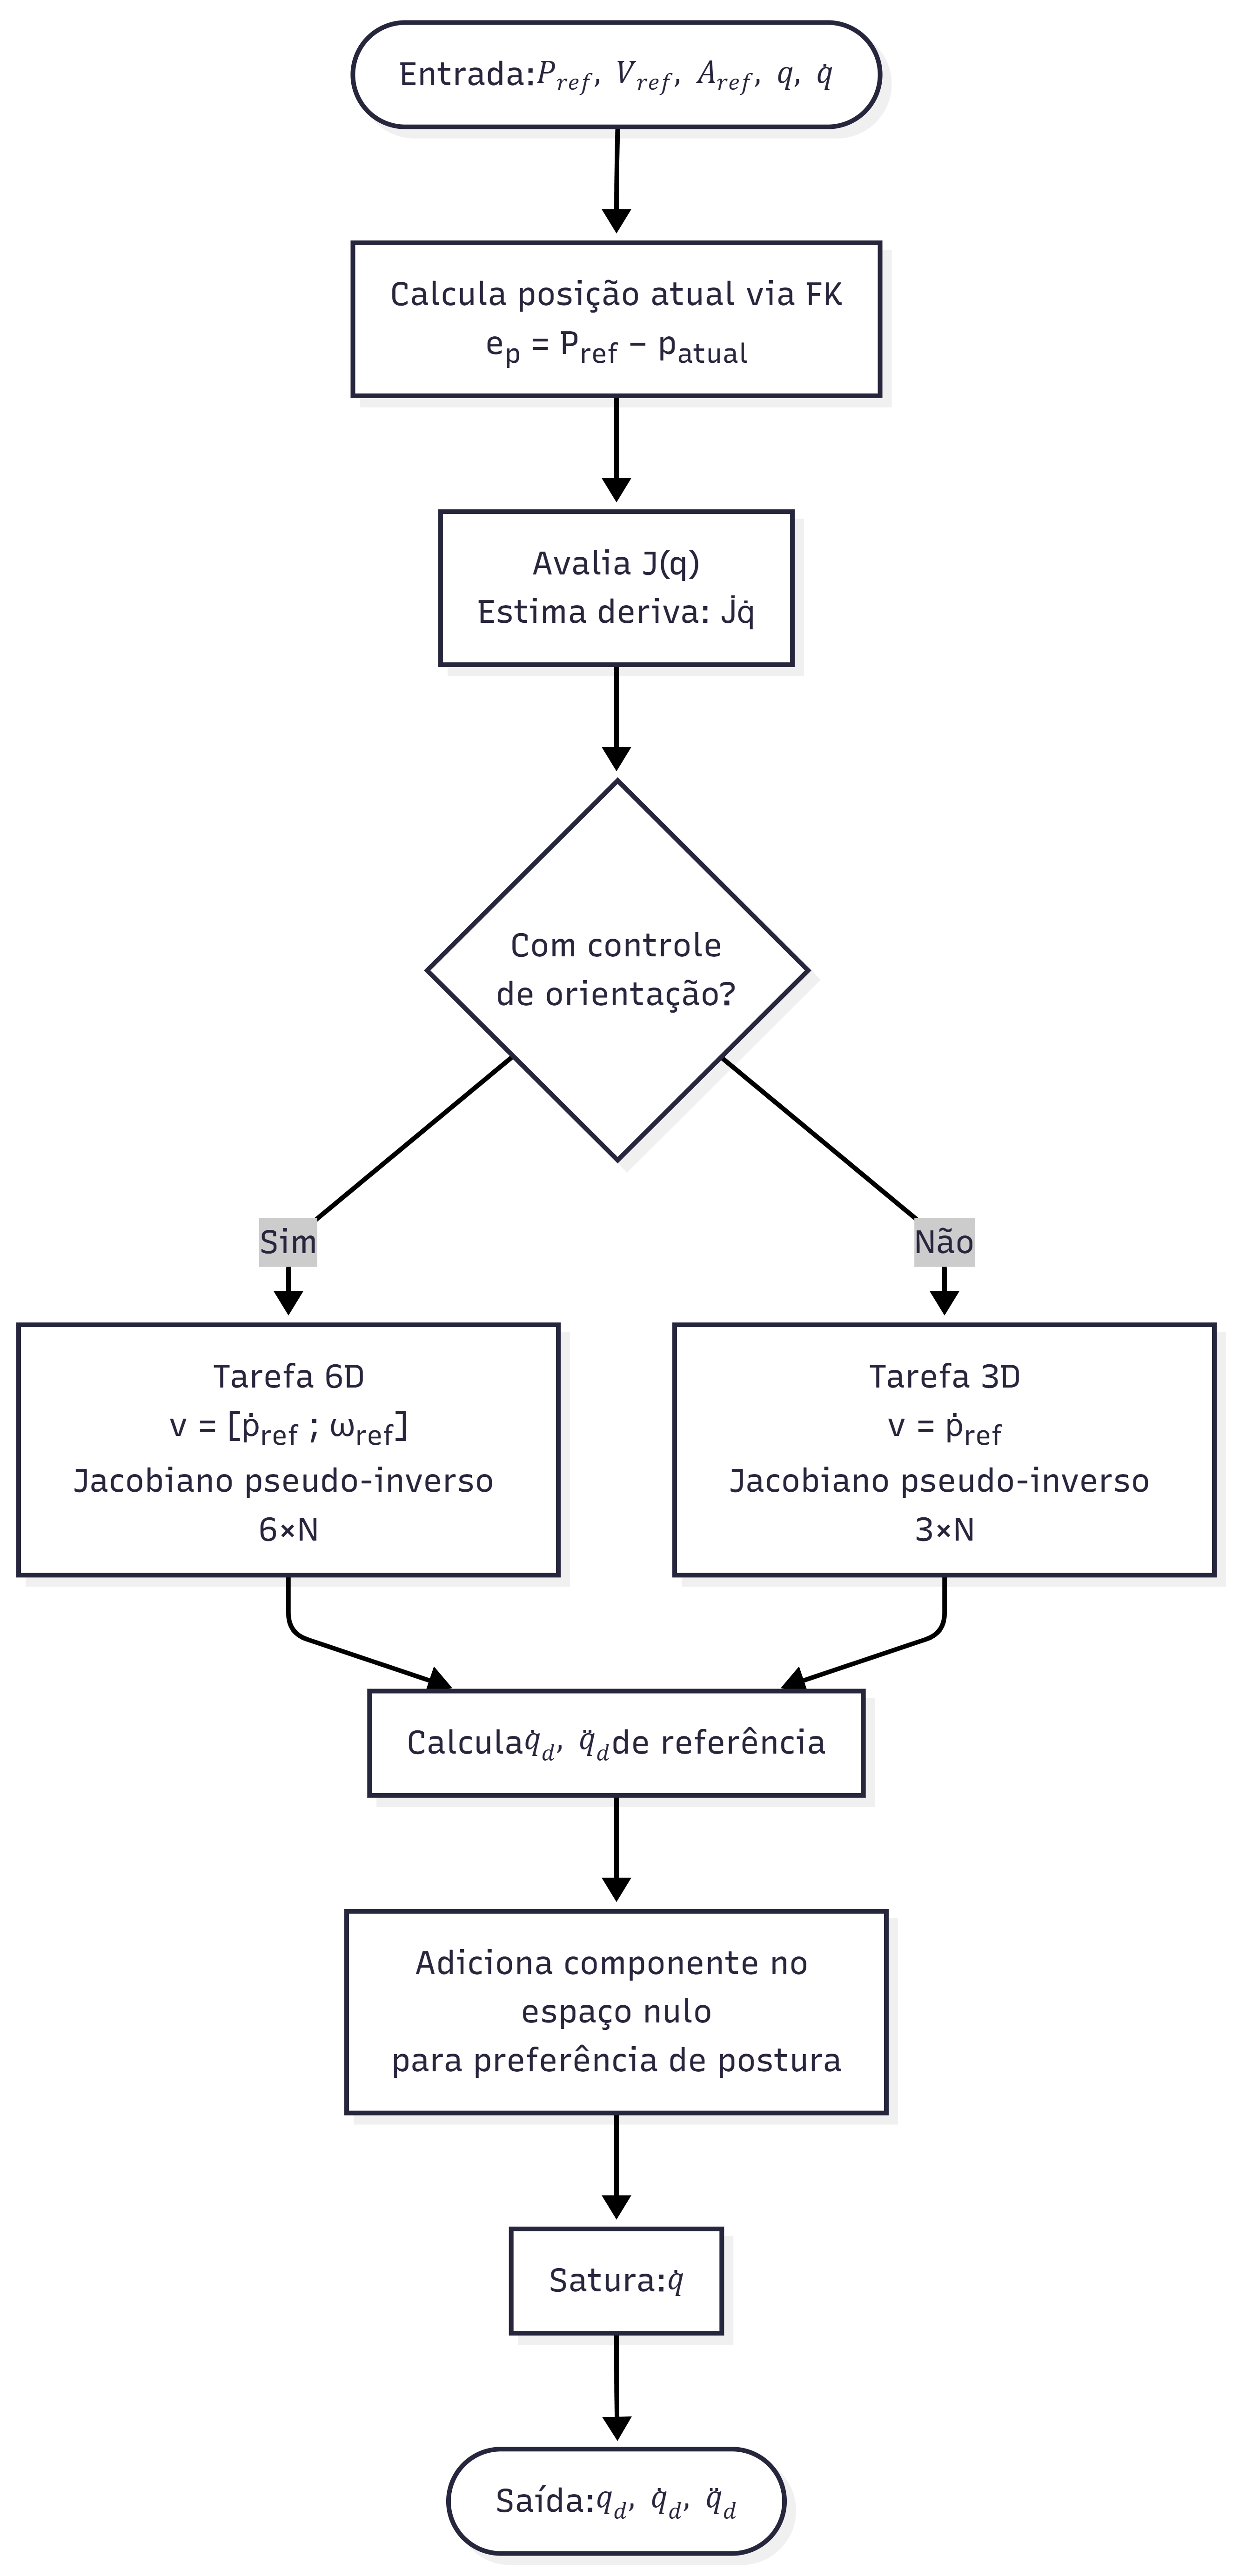
\includegraphics[width=0.7\textwidth]{figuras/Diagramas/Diagrama 6a — CLIK Cinemática Inversa Numérica.png}
    \caption{Fluxo do algoritmo CLIK (\textit{Closed-Loop Inverse Kinematics}) implementado no \textit{Hephaestus}: recebe as referências cartesianas $\{P_{\text{ref}}, \dot{P}_{\text{ref}}, \ddot{P}_{\text{ref}}\}$ e produz as referências de junta $\{q_d, \dot{q}_d, \ddot{q}_d\}$ por pseudo-inversão amortecida DLS (Equação~\eqref{eq:dls_pos}) com gestão de redundância por projeção no espaço nulo \cite{chiaverini1994review, nakamura1986inverse, chiaverini1997singularity}.}
    \label{fig:clik_cinematica}
\end{figure}

% ==============================================================================
\section{Integrador Simplético de Euler com Substeps}
\label{sec:integrador}
% ==============================================================================

\subsection{Hierarquia de Passos de Tempo}

O integrador numérico opera em dois níveis de passo de tempo, independentes entre si:

\begin{itemize}
    \item $\Delta t_{\text{phys}}$: passo de integração física, tipicamente $\Delta t_{\text{phys}} = 10^{-3}$ s. Determina a fidelidade numérica da integração das equações de movimento.
    \item $\Delta t_{\text{vis}}$: passo de amostragem para visualização e armazenamento de resultados, tipicamente $\Delta t_{\text{vis}} = 5 \times 10^{-2}$ s. Determina a taxa de frames da animação.
\end{itemize}

O número de \textit{substeps} por frame de visualização é:
\begin{equation}
    N_s = \left\lceil \frac{\Delta t_{\text{vis}}}{\Delta t_{\text{phys}}} \right\rceil,
    \label{eq:substeps}
\end{equation}
e o $\Delta t_{\text{vis}}$ efetivo é ajustado para $N_s \cdot \Delta t_{\text{phys}}$, garantindo que o passo visual seja um múltiplo inteiro do físico. Essa separação permite aumentar a fidelidade numérica sem custo proporcional de armazenamento ou renderização: para $\Delta t_{\text{vis}} = 0.05$ s e $\Delta t_{\text{phys}} = 10^{-3}$ s, obtêm-se 50 substeps por frame, com apenas um frame armazenado por cada 50 avaliações de dinâmica \cite{leimkuhler2004simulating}.

\subsection{Integrador Simplético de Euler}

A integração das equações de movimento \eqref{eq:motion_equation} (Capítulo~\ref{cap:revisao}) é realizada pelo método de Euler Simplético de primeira ordem. A cada substep físico, a dinâmica direta é resolvida por:
\begin{equation}
    \ddot{q}^n = M^{-1}\!\left(q^n\right)\left[\tau^n_{\text{ctrl}} + \tau^n_{\text{dist}} - C^n - G^n - \tau^n_{\text{pass}}\right],
    \label{eq:dyn_direct}
\end{equation}
onde $\tau^n_{\text{ctrl}}$ é o torque do controlador, $\tau^n_{\text{dist}}$ é o torque de distúrbio externo (opcional), $\tau^n_{\text{pass}}$ reúne as forças passivas (atrito + arrasto, descritos na Seção~\ref{sec:dissipative}), e $C^n$, $G^n$ são avaliados na configuração atual $(q^n, \dot{q}^n)$. A inversão de $M$ é realizada por \texttt{np.linalg.solve}, que utiliza decomposição LU — numericamente mais estável e eficiente que o cálculo explícito da inversa \cite{golub2013matrix}.

A atualização do estado segue a sequência simplética:
\begin{align}
    \dot{q}^{n+1} &= \dot{q}^n + \ddot{q}^n\,\Delta t_{\text{phys}}, \label{eq:symplectic1}\\
    q^{n+1} &= q^n + \dot{q}^{n+1}\,\Delta t_{\text{phys}}. \label{eq:symplectic2}
\end{align}

A ordem em que velocidade e posição são atualizadas — velocidade \emph{antes} da posição — distingue o integrador simplético do Euler explícito padrão. Enquanto o Euler explícito acumula energia seculamente (instabilidade numérica suave), o Euler Simplético preserva uma ``energia modificada'' próxima da hamiltoniana real do sistema, garantindo estabilidade de longo prazo \cite{leimkuhler2004simulating, hairer2006geometric}. Para simulações de controle em malha fechada com duração moderada (tipicamente $< 30$ s), essa diferença é crítica para a fidelidade dos torques calculados e da resposta do controlador.

Após cada atualização, as coordenadas de juntas rotacionais são restritas ao intervalo $(-\pi, \pi]$ pelo operador de envolvimento (\textit{wrap}):
\begin{equation}
    q_i \leftarrow (q_i + \pi) \bmod 2\pi - \pi, \quad \forall i \text{ tal que a junta } i \text{ é rotacional},
    \label{eq:wrap}
\end{equation}
assegurando que os erros de junta $e_i = q_{d,i} - q_i$ representem sempre o menor caminho angular — condição necessária para a estabilidade de controladores com ganho proporcional \cite{spong2020robot}. Uma verificação de finitude (\texttt{np.isfinite}) é aplicada a $q$ e $\dot{q}$ após cada substep; caso valores NaN ou Inf sejam detectados, a simulação é interrompida com uma exceção descritiva, prevenindo propagação silenciosa de instabilidades numéricas.

% ==============================================================================
\section{Estratégias de Controle Não-Linear}
\label{sec:controle_impl}
% ==============================================================================

Quatro estratégias de controle não-linear são implementadas no \textit{Hephaestus}, todas recebendo como entrada as referências de junta $\{q_d, \dot{q}_d, \ddot{q}_d\}$ geradas pelo CLIK e as matrizes dinâmicas avaliadas numericamente. Uma única interface unificada — o parâmetro \texttt{ctrl\_params} do método \texttt{run()} — seleciona e configura o controlador ativo, permitindo a comparação direta das estratégias sob condições idênticas de trajetória, modelo e perturbações.

\subsection{Controle por Torque Computado com PID (CTC-PID)}

O Controle por Torque Computado com PID \cite{craig1989introduction, spong2020robot} é a estratégia padrão do simulador. A lei de controle é:
\begin{equation}
    \tau_{\text{CTC-PID}} = M(q)\left[\ddot{q}_d + K_D\dot{e} + K_P e + K_I \int e\,dt\right] + C(q,\dot{q}) + G(q),
    \label{eq:ctc_pid_impl}
\end{equation}
onde $e = q_d - q$, $K_P = k_p I_N$, $K_D = 2\zeta\sqrt{k_p} I_N$ (criticamente amortecido para $\zeta = 1$) e $K_I = k_i I_N$. O ganho derivativo é derivado automaticamente do proporcional pelo método do polinômio característico de segunda ordem, garantindo amortecimento crítico para qualquer valor de $k_p$ \cite{astrom1995theory}.

O integrador é sujeito a \textit{anti-windup} por clamping:
\begin{equation}
    \int e\,dt \leftarrow \text{clip}\!\left(\int e\,dt + e\,\Delta t,\;  -e_{\max},\; e_{\max}\right),
    \label{eq:antiwindup}
\end{equation}
onde $e_{\max}$ é o limite de \textit{windup} configurável, que previne a acumulação do integrador durante períodos de saturação do atuador \cite{astrom1995theory}. Com modelo dinâmico exato, a lei CTC cancela a não-linearidade e a dinâmica de erro satisfaz $\ddot{e} + K_D\dot{e} + K_P e = 0$, que é um sistema linear estável de segunda ordem \cite{craig1989introduction}.

\subsection{Controle por Modo Deslizante (CT-SMC)}

O Controle por Modo Deslizante \cite{slotine1991applied} define a superfície deslizante:
\begin{equation}
    S = \dot{e} + \lambda e, \qquad e = q - q_d,
    \label{eq:sliding_surface}
\end{equation}
e a lei de controle baseada em modelo:
\begin{equation}
    \tau_{\text{SMC}} = M(q)\left[\ddot{q}_{d,f} - \lambda\dot{e} - K\tanh(S/\phi)\right] + C(q,\dot{q}) + G(q),
    \label{eq:smc_impl}
\end{equation}
onde $\ddot{q}_{d,f} = \alpha\,\ddot{q}_d + (1-\alpha)\,\ddot{q}_{d,f}^{\text{prev}}$ é um filtro passa-baixas da aceleração de referência com coeficiente $\alpha \in (0,1]$. O filtro atenua picos de aceleração oriundos das derivadas do CLIK, que seriam amplificados pelo ganho $\lambda$ na lei de controle — uma instabilidade prática frequentemente não mencionada nas formulações teóricas do CT-SMC \cite{slotine1991applied, edwards1998sliding}.

A função $\tanh(S/\phi)$ substitui o sinal descontínuo $\text{sign}(S)$ pela camada limite de espessura $\phi > 0$, eliminando o \textit{chattering} (oscilações de alta frequência) ao custo de uma robustez assintótica dentro da camada \cite{slotine1991applied}. A análise formal da robustez com camada limite foi conduzida por Burton e Zinober \cite{burton1986continuous}: para perturbações $|d| \leq D$, o erro de regime permanente é limitado por $\|S\|_\infty \leq \phi \cdot D / K$, o que permite ao projetista estabelecer um compromisso explícito entre \textit{chattering} e precisão de rastreamento.

\subsection{Super-Twisting (STA)}

O algoritmo Super-Twisting (STA), proposto por Levant \cite{levant1993sliding}, é um modo deslizante de segunda ordem que elimina o \textit{chattering} intrinsecamente ao produzir um sinal de controle contínuo. A superfície deslizante é idêntica à Equação~\eqref{eq:sliding_surface}, e a parcela de modo deslizante é:
\begin{align}
    v_{\text{sw}} &= -k_1\,|S|^{1/2}\,\text{sign}(S) + z, \label{eq:sta1_impl}\\
    \dot{z} &= -k_2\,\text{sign}(S), \label{eq:sta2_impl}
\end{align}
onde $z$ é uma variável interna integrada numericamente por Euler explícito: $z^{n+1} = z^n - k_2\,\text{sign}(S^n)\,\Delta t$. A lei de controle completa é:
\begin{equation}
    \tau_{\text{STA}} = M(q)\left[\ddot{q}_{d,f} - \lambda\dot{e} + v_{\text{sw}}\right] + C(q,\dot{q}) + G(q).
    \label{eq:sta_ctrl}
\end{equation}

O sinal $v_{\text{sw}}$ é contínuo porque $z$ integra o sinal descontínuo, fazendo $v_{\text{sw}}$ variar continuamente mesmo que $\text{sign}(S)$ seja descontínuo. Moreno e Osorio \cite{moreno2012strict} forneceram uma função de Lyapunov estrita para o STA, estabelecendo condições de ganho suficientes para convergência em tempo finito com distúrbio de derivada limitada $|\dot{d}| \leq \delta$: $k_2 > \delta$ e $k_1 > 2\sqrt{k_2\,\delta}$. A convergência em tempo finito de $S \to 0$ e $\dot{S} \to 0$ diferencia qualitativamente o STA do CT-SMC de primeira ordem, cuja convergência é assintótica \cite{levant1993sliding, utkin2017sliding}.

O filtro de $\ddot{q}_{d,f}$ é compartilhado com a implementação do CT-SMC, sendo parametrizado pelo mesmo coeficiente $\alpha$, o que garante comparabilidade direta das duas estratégias quando $\lambda$, $K$ (CT-SMC) e $k_1$, $k_2$ (STA) são ajustados para desempenhos nominais equivalentes.

\subsection{Controle por Rejeição Ativa de Distúrbios Linear (LADRC)}

O LADRC (Linear Active Disturbance Rejection Control), proposto por Han \cite{han1995class} e formalizado em versão linear por Gao \cite{gao2003scaling}, é implementado de forma descentralizada — um ESO e uma lei de controle por junta, ignorando o acoplamento dinâmico \cite{huang2014active}. Para a junta $i$, a dinâmica nominal é reescrita como:
\begin{equation}
    \ddot{q}_i = b_{0,i}\,\tau_i + f_i, \qquad f_i = \text{distúrbio total},
    \label{eq:adrc_plant_impl}
\end{equation}
onde $b_{0,i} \approx 1/M_{ii}(q_0)$ é estimado automaticamente a partir da diagonal da matriz de inércia na postura inicial, conforme a opção \texttt{auto\_b0} da configuração.

O ESO de terceira ordem (linear) é integrado por Euler explícito a cada passo $\Delta t_{\text{phys}}$:
\begin{align}
    z_1^{n+1} &= z_1^n + \Delta t\left[z_2^n - \beta_1(z_1^n - q_i^n)\right], \label{eq:eso1_impl}\\
    z_2^{n+1} &= z_2^n + \Delta t\left[z_3^n - \beta_2(z_1^n - q_i^n) + b_0 \tau_i^{n-1}\right], \label{eq:eso2_impl}\\
    z_3^{n+1} &= z_3^n - \Delta t\,\beta_3(z_1^n - q_i^n), \label{eq:eso3_impl}
\end{align}
com $\beta_1 = 3\omega_o$, $\beta_2 = 3\omega_o^2$, $\beta_3 = \omega_o^3$ \cite{gao2003scaling}. A frequência $\omega_o$ é automaticamente limitada por $\omega_o \leq \omega_{\max}/\Delta t$ para garantir estabilidade numérica do ESO discreto: a condição $\omega_o \Delta t \leq 0.1$ é aplicada como heurística de projeto \cite{zheng2010practical}.

A estimativa $z_3^n$ do distúrbio total é suavizada por um filtro IIR de primeira ordem antes de ser usada na lei de controle:
\begin{equation}
    z_3^{\text{filt},n} = \alpha_{\text{filt}}\,z_3^n + (1 - \alpha_{\text{filt}})\,z_3^{\text{filt},n-1},
    \label{eq:z3_filter}
\end{equation}
onde $\alpha_{\text{filt}} \in (0, 1]$ é o coeficiente do filtro ($\alpha = 1$ desativa o filtro). Este filtro é necessário em prática para atenuar o conteúdo de alta frequência que o ESO amplifica nos ciclos iniciais, antes de convergir ao valor real de $f_i$ \cite{han2009pid}.

A lei de controle cancela o distúrbio estimado e acrescenta \textit{feedforward} explícito de $G$ e $C$ para reduzir o distúrbio residual que o ESO precisa estimar:
\begin{equation}
    \tau_i^{\text{LADRC}} = \frac{u_{0,i} - z_{3,i}^{\text{filt}}}{b_{0,i}} + G_i + C_i,
    \label{eq:ladrc_ctrl}
\end{equation}
\begin{equation}
    u_{0,i} = \ddot{q}_{d,i} + k_{p,i}(q_{d,i} - q_i) + k_{d,i}(\dot{q}_{d,i} - \dot{q}_i).
    \label{eq:ladrc_u0}
\end{equation}

O \textit{feedforward} de $G$ e $C$ é especialmente crítico em manipuladores terrestres (onde $G \neq 0$) e no início de trajetórias rápidas (onde $C \propto \dot{q}^2$ cresce rapidamente): sem esses termos, o ESO deve perseguir um distúrbio crescente com lag dinâmico, introduzindo um transiente oscilatório nos primeiros instantes da trajetória. A inclusão do feedforward reduz o distúrbio residual a apenas erros de modelo e perturbações externas — sinais pequenos e quase constantes que o ESO estima com precisão \cite{han2009pid}. A análise de estabilidade do LADRC com esta formulação foi formalizada por Zheng e Gao \cite{zheng2010practical}.

% ==============================================================================
\section{Modelos de Forças Dissipativas}
\label{sec:dissipative}
% ==============================================================================

\subsection{Atrito nas Juntas}

O modelo de atrito nas juntas combina os componentes de Coulomb (atrito estático/cinético) e viscoso (proporcional à velocidade):
\begin{equation}
    \tau_{\text{fric},i} = F_{c,i}\,\tanh\!\left(\frac{\dot{q}_i}{\varepsilon}\right) + B_{v,i}\,\dot{q}_i,
    \label{eq:friction}
\end{equation}
onde $F_{c,i} \geq 0$ é o coeficiente de atrito de Coulomb por junta, $B_{v,i} \geq 0$ é o coeficiente viscoso e $\varepsilon > 0$ é a zona suave (\textit{regularization zone}). O uso de $\tanh$ em vez de $\text{sign}(\dot{q})$ é essencial para evitar descontinuidades que causariam instabilidade numérica no integrador: para $|\dot{q}_i| \gg \varepsilon$, $\tanh(\dot{q}_i/\varepsilon) \approx \text{sign}(\dot{q}_i)$, recuperando o comportamento de Coulomb clássico; para $|\dot{q}_i| \approx 0$, a transição é suave e impede o fenômeno de \textit{stiction} numérico \cite{slotine1991applied}. O valor padrão $\varepsilon = 0.05$ rad/s é calibrado para suavizar sem mascarar a zona de atrito estático em velocidades de junta típicas de manipuladores de laboratório.

\subsection{Arrasto Hidrodinâmico}

No modo \textit{Hydro}, um modelo simplificado de arrasto no espaço de juntas é aplicado como força passiva \cite{fossen2011handbook, antonelli2014modelling}:
\begin{equation}
    \tau_{\text{drag},i} = D_{\text{lin},i}\,\dot{q}_i + D_{\text{quad},i}\,|\dot{q}_i|\,\dot{q}_i,
    \label{eq:drag_impl}
\end{equation}
onde $D_{\text{lin},i}$ e $D_{\text{quad},i}$ são os coeficientes de arrasto linear e quadrático da junta $i$. Esta formulação é equivalente à Equação~\eqref{eq:drag} do Capítulo~\ref{cap:revisao}, parametrizada no espaço de juntas em vez do espaço cartesiano para compatibilidade com o integrador \cite{antonelli2014modelling}. O arrasto quadrático captura os efeitos de pressão (regime turbulento, número de Reynolds elevado) que dominam em velocidades de junta mais altas, enquanto o linear captura o arrasto viscoso do escoamento laminar em baixas velocidades \cite{fossen2011handbook, newman1977marine}.

Ambas as forças dissipativas são aplicadas na equação de dinâmica direta como torques passivos externos:
\begin{equation}
    \ddot{q}^n = M^{-1}\!\left(\tau_{\text{ctrl}}^n - C^n - G^n - \tau_{\text{fric}}^n - \tau_{\text{drag}}^n\right),
    \label{eq:dyn_complete}
\end{equation}
fora do laço do controlador. Essa separação é fisicamente correta: os torques dissipativos são forças do ambiente (não cancelas pelo controlador a priori) e devem ser observados ou estimados para serem compensados — papel que o ESO do LADRC desempenha implicitamente \cite{han2009pid, huang2014active}.

% ==============================================================================
\section{Paralelismo na Avaliação Numérica}
\label{sec:parallel_sim}
% ==============================================================================

A avaliação numérica das funções $f_M$, $f_C$ e $f_G$ a cada passo de integração é o principal gargalo de tempo de execução para sistemas com $N \geq 5$ GDL, onde as expressões compiladas possuem centenas de operações trigonométricas e matriciais. Para mitigar esse custo, o \textit{Hephaestus} suporta avaliação paralela via um executor persistente de processos.

O executor \texttt{ProcessPoolExecutor} é inicializado uma única vez após a compilação (método \texttt{warm\_up\_workers()}), com cada \textit{worker} executando o inicializador \texttt{\_init\_worker} que compila localmente as três funções via \texttt{lambdify} e as armazena no dicionário de módulo \texttt{\_WORKER\_FUNCS}. A cada passo físico, três tarefas são submetidas em paralelo:
\begin{equation}
    \texttt{futures} = \left\{
        M: \texttt{executor.submit}(\texttt{\_eval\_worker}, (\text{"M"}, \textbf{args})), \;
        C: \texttt{executor.submit}(\ldots), \;
        G: \texttt{executor.submit}(\ldots)
    \right\},
    \label{eq:parallel_submit}
\end{equation}
e os resultados são coletados por \texttt{Future.result()} após o despacho das três tarefas, aproveitando a sobreposição de computação \cite{beazley2010understanding}.

A chave da eficiência é a \textbf{persistência} do executor: ao contrário de uma implementação ingênua que instancia e destrói um \textit{pool} por simulação (custo de 2--8 s por instância, conforme medido nos testes), o executor é instanciado uma única vez e reutilizado em todas as chamadas subsequentes a \texttt{run()}. A detecção de mudança no número de \textit{workers} solicita reinicialização automática do executor, garantindo flexibilidade sem custo desnecessário \cite{leu1986automated}.

Quando o paralelismo não está habilitado (\texttt{use\_parallel=False}), as três funções são avaliadas sequencialmente na thread principal — comportamento padrão seguro para executáveis PyInstaller, máquinas com um único núcleo ou ambientes de depuração. Esta opção também é preferida para sistemas com $N \leq 4$ GDL, onde o \textit{overhead} de IPC supera o ganho de paralelismo \cite{beazley2010understanding}.

% ==============================================================================
\section{Verificação de Estabilidade Numérica}
\label{sec:estabilidade_num}
% ==============================================================================

A estabilidade numérica do integrador simplético é governada pela relação entre o passo de integração $\Delta t_{\text{phys}}$ e as frequências naturais do sistema em malha fechada. Para o CTC, a dinâmica de erro é linear de segunda ordem com frequência natural $\omega_n = \sqrt{k_p}$; a condição de estabilidade de Euler simplético exige \cite{leimkuhler2004simulating}:
\begin{equation}
    \Delta t_{\text{phys}} < \frac{2}{\omega_n} = \frac{2}{\sqrt{k_p}},
    \label{eq:stability_condition}
\end{equation}
ou seja, ao menos dois passos por período de oscilação de malha fechada. Para $k_p = 100$ rad$^2$/s$^2$ (ganho típico), $\omega_n = 10$ rad/s e $\Delta t_{\text{phys}} < 0.2$ s — condição satisfeita com folga para $\Delta t_{\text{phys}} = 10^{-3}$ s \cite{hairer2006geometric}. Avisos automáticos são emitidos quando $\Delta t_{\text{phys}} > 10^{-2}$ s ou $\Delta t_{\text{vis}} > 0.1$ s, alertando o usuário sobre potencial instabilidade.

Para o LADRC, a condição adicional de estabilidade do ESO discreto é $\omega_o \Delta t_{\text{phys}} \leq 0.1$, correspondente à frequência de observador máxima $\omega_o^{\max} = 0.1/\Delta t_{\text{phys}} = 100$ rad/s para $\Delta t_{\text{phys}} = 10^{-3}$ s. Este limite é imposto automaticamente pela verificação \texttt{max\_wo\_dt} no construtor do LADRC \cite{zheng2010practical}.

% ==============================================================================
\section{Síntese do Capítulo}
% ==============================================================================

Este capítulo descreveu a arquitetura completa de simulação numérica do \textit{Hephaestus}. O fluxo de execução do método \texttt{run()} integra, em uma única interface unificada, as seguintes contribuições:

\begin{itemize}
    \item \textbf{Planejamento de trajetória} com polinômio cúbico, suportando segmentos lineares e arcos circulares com aceleração \textit{feedforward} analítica e seis modos de referência de orientação, incluindo SLERP geodésico \cite{shoemake1985animating} e controle tangencial.
    \item \textbf{Inicialização robusta} por Levenberg-Marquardt com busca em linha adaptativa \cite{marquardt1963algorithm, armijo1966minimization}, garantindo partida a partir de qualquer configuração factível.
    \item \textbf{CLIK estendido ao espaço 6D}, com \textit{feedforward} de velocidade e aceleração, correção de deriva do Jacobiano, tratamento de singularidades por DLS \cite{nakamura1986inverse} e gestão de redundância via espaço nulo \cite{chiaverini1997singularity, liegeois1977automatic}.
    \item \textbf{Integrador simplético de Euler} com \textit{substeps} independentes da taxa de visualização, garantindo estabilidade de energia a longo prazo e alta fidelidade numérica \cite{leimkuhler2004simulating, hairer2006geometric}.
    \item \textbf{Quatro controladores não-lineares} comparáveis: CTC-PID \cite{craig1989introduction, astrom1995theory}, CT-SMC com camada limite \cite{slotine1991applied, burton1986continuous}, Super-Twisting STA com convergência em tempo finito \cite{levant1993sliding, moreno2012strict} e LADRC descentralizado com ESO de terceira ordem \cite{gao2003scaling, zheng2010practical, huang2014active}.
    \item \textbf{Forças dissipativas} de atrito nas juntas (Coulomb + viscoso, suavizado por $\tanh$) e arrasto hidrodinâmico (linear + quadrático) \cite{fossen2011handbook, antonelli2014modelling}, aplicadas separadamente do controle para máxima fidelidade física.
    \item \textbf{Executor paralelo persistente} para avaliação paralela de $M$, $C$, $G$ a cada substep, com custo de \textit{spawn} amortizado sobre toda a simulação \cite{beazley2010understanding, leu1986automated}.
\end{itemize}

O Capítulo seguinte apresenta os resultados experimentais obtidos com a plataforma \textit{Hephaestus} em dois cenários de validação: um manipulador serial de 3 GDL em ambiente terrestre e um UVMS de 6 GDL em ambiente subaquático, comparando as quatro estratégias de controle em termos de erro de rastreamento, torques requeridos e resposta a perturbações externas.

  \chapter{Controladores Implementados e Integração com o Modelo}
\label{cap:controladores}

Este capítulo aprofunda a análise dos quatro controladores não-lineares implementados no \textit{Hephaestus} sob a perspectiva da integração com o modelo dinâmico simbólico derivado no Capítulo~\ref{cap:modelagem}. Enquanto o Capítulo~\ref{cap:simulacao} descreveu a arquitetura de simulação e apresentou as leis de controle de forma operacional, este capítulo concentra-se em três aspectos complementares: (i) a fundamentação teórica aprofundada de cada estratégia, com provas ou condições formais de estabilidade; (ii) a análise da integração específica entre cada controlador e as matrizes $M(q)$, $C(q,\dot{q})$, $G(q)$ geradas simbolicamente; e (iii) uma comparação sistemática das quatro estratégias em termos de robustez a incertezas paramétricas, sensibilidade a perturbações externas e compromissos de ajuste de ganhos.

% ==============================================================================
\section{Estrutura Unificada de Controle em Malha Fechada}
\label{sec:ctrl_framework}
% ==============================================================================

A arquitetura de controle do \textit{Hephaestus} segue o paradigma de \textit{controle baseado em modelo} (\textit{model-based control}), no qual o conhecimento das equações de movimento do robô é explorado explicitamente na lei de controle para cancelar ou compensar a não-linearidade intrínseca da dinâmica \cite{craig1987introduction, spong2020robot, siciliano2009robotics}. O fluxo de sinais é organizado em três camadas sobrepostas, conforme ilustrado na Figura~\ref{fig:ctrl_framework}:

\begin{enumerate}
    \item \textbf{Camada de Planejamento} (trajetória cartesiana $\to$ CLIK $\to$ referências de junta): gera as triplas $\{q_d(t), \dot{q}_d(t), \ddot{q}_d(t)\}$ a cada passo de integração, conforme descrito nas Seções~\ref{sec:traj_planning} e \ref{sec:clik} do Capítulo~\ref{cap:simulacao}.
    \item \textbf{Camada de Controle} (referências de junta + estado medido $\to$ torque de controle $\tau_{\text{ctrl}}$): implementa uma das quatro estratégias descritas neste capítulo, consumindo as matrizes dinâmicas $M$, $C$, $G$ avaliadas numericamente.
    \item \textbf{Camada de Integração} (torque total $\to$ integrador simplético $\to$ próximo estado): resolve a dinâmica direta $\ddot{q} = M^{-1}(\tau_{\text{ctrl}} + \tau_{\text{dist}} - C - G - \tau_{\text{pass}})$ e atualiza o estado $(q, \dot{q})$.
\end{enumerate}

\begin{figure}[h!]
\centering
\begin{tikzpicture}[
    block/.style={rectangle, draw, minimum width=2.6cm, minimum height=0.8cm, align=center, font=\small},
    sum/.style={circle, draw, minimum size=0.5cm},
    arr/.style={->, >=stealth, thick}
]
    \node[block] (traj) {Planejamento\\de Trajetória};
    \node[block, right=1.0cm of traj] (clik) {CLIK};
    \node[block, right=1.0cm of clik] (ctrl) {Controlador\\($\tau_{\text{ctrl}}$)};
    \node[block, right=1.0cm of ctrl] (plant) {Planta\\$M\ddot{q}+C\dot{q}+G=\tau$};
    \node[block, below=0.7cm of ctrl] (model) {Modelo\\$M,C,G$};
    \draw[arr] (traj) -- node[above]{\small$P_{\text{ref}},\dot{P}_{\text{ref}},\ddot{P}_{\text{ref}}$} (clik);
    \draw[arr] (clik) -- node[above]{\small$q_d,\dot{q}_d,\ddot{q}_d$} (ctrl);
    \draw[arr] (ctrl) -- node[above]{\small$\tau$} (plant);
    \draw[arr] (model) -- (ctrl);
    \draw[arr] (plant.east) -- ++(0.5,0) |- node[right, pos=0.25]{\small$q,\dot{q}$} (clik.south |- plant.east -| clik.east) -- (clik.east);
    \draw[arr] (plant.south) |- (model.east);
\end{tikzpicture}
\caption{Estrutura de controle em malha fechada do \textit{Hephaestus}. O modelo dinâmico simbólico-numérico alimenta diretamente a camada de controle e é avaliado no estado corrente $(q^n, \dot{q}^n)$ a cada passo físico.}
\label{fig:ctrl_framework}
\end{figure}

A interface de seleção de controlador é estabelecida pelo parâmetro \texttt{ctrl\_params} do método \texttt{run()}, cujo campo \texttt{"type"} determina qual classe de controlador é instanciada. Essa interface unificada permite a comparação direta das quatro estratégias sob condições rigorosamente idênticas de trajetória, modelo, perturbações e passo de integração — requisito metodológico fundamental para estudos comparativos em robótica de controle \cite{moura2020educational, astrom1995pid}.

A disponibilidade das matrizes $M(q)$, $C(q,\dot{q})$ e $G(q)$ como funções numéricas compiladas (Seção~\ref{sec:lambdify_cse} do Capítulo~\ref{cap:modelagem}) é o que torna o controle baseado em modelo computacionalmente viável em tempo real. Sem a compilação via \texttt{lambdify} com CSE, a avaliação simbólica de $M$ a cada passo de integração seria proibitivamente lenta — na ordem de segundos por avaliação, contra microsegundos com a função compilada. Essa ponte entre a computação simbólica e numérica é o elemento técnico central que diferencia o \textit{Hephaestus} de simuladores que adotam modelos numéricos fixos \cite{harrington2019automated}.

% ==============================================================================
\section{Controle por Torque Computado com PID}
\label{sec:ctc_pid_cap5}
% ==============================================================================

\subsection{Fundamentação Teórica e Cancelamento de Não-Linearidade}

O Controle por Torque Computado (CTC), também denominado \textit{computed torque control} ou \textit{feedback linearization} \cite{isidori1995nonlinear, khalil2002nonlinear}, é a estratégia de referência do \textit{Hephaestus} e o ponto de partida para a compreensão das demais. A lei de controle fundamenta-se no cancelamento algébrico da dinâmica não-linear do robô pela inversão explícita do modelo:
\begin{equation}
    \tau_{\text{CTC}} = M(q)\,v + C(q,\dot{q}) + G(q),
    \label{eq:ctc_geral}
\end{equation}
onde $v \in \mathbb{R}^N$ é um sinal de controle auxiliar linear \cite{spong2020robot}. Substituindo a Equação~\eqref{eq:ctc_geral} na equação de movimento $M\ddot{q} + C\dot{q} + G = \tau$ e assumindo modelo exato, obtém-se a dinâmica de malha fechada linearizada:
\begin{equation}
    \ddot{q} = v,
    \label{eq:ctc_linear}
\end{equation}
que é um sistema de integradores duplos desacoplados e independentes da configuração $q$. A não-linearidade e o acoplamento entre juntas são completamente eliminados por \textit{feedback linearization} exata, desde que $M(q)$, $C(q,\dot{q})$ e $G(q)$ sejam conhecidos exatamente \cite{spong2020robot, isidori1995nonlinear}.

Com a escolha do sinal auxiliar PID:
\begin{equation}
    v = \ddot{q}_d + K_D\dot{e} + K_P e + K_I \int_0^t e\,d\tau,
    \label{eq:v_pid}
\end{equation}
onde $e = q_d - q$ é o erro de junta, a dinâmica de erro satisfaz:
\begin{equation}
    \ddot{e} + K_D\dot{e} + K_P e + K_I \int_0^t e\,d\tau = 0.
    \label{eq:error_dyn_pid}
\end{equation}

Esta é a equação de um sistema linear de terceira ordem com coeficientes matriciais diagonais constantes. Sua estabilidade é garantida pelas condições de Routh-Hurwitz sobre os ganhos $\{K_P, K_D, K_I\}$ \cite{astrom1995pid, ogata2010modern}: para $K_I = 0$ (modo PD), a condição é simplesmente $K_P > 0$ e $K_D > 0$. A escolha $K_D = 2\zeta\sqrt{K_P}$ com $\zeta = 1$ impõe amortecimento crítico ao sistema de segunda ordem resultante, minimizando o \textit{overshoot} enquanto maximiza a velocidade de convergência para $K_I = 0$ \cite{astrom1995pid}.

\subsection{Integração com o Modelo Simbólico-Numérico}

No \textit{Hephaestus}, os termos $M(q)$, $C(q,\dot{q})$ e $G(q)$ são avaliados numericamente pelas funções compiladas \texttt{func\_M}, \texttt{func\_C} e \texttt{func\_G} (Seção~\ref{sec:lambdify_cse} do Capítulo~\ref{cap:modelagem}), com os argumentos construídos pelo método \texttt{\_build\_args(q, dq)}. Essa avaliação ocorre a cada passo de integração física $\Delta t_{\text{phys}} = 10^{-3}$ s, garantindo que o controlador utilize o modelo atualizado na configuração corrente do robô. A operação de maior custo computacional é a resolução do sistema linear $M\,\ddot{q} = \tau - C - G$ via \texttt{np.linalg.solve} (decomposição LU), com complexidade $O(N^3)$ por passo \cite{golub2013matrix}.

\subsection{Análise de Robustez a Incertezas Paramétricas}

A fragilidade fundamental do CTC é sua dependência do modelo exato. Em presença de erros de modelagem $\Delta M$, $\Delta C$, $\Delta G$, a dinâmica de malha fechada torna-se:
\begin{equation}
    \ddot{e} + K_D\dot{e} + K_P e = \underbrace{M^{-1}(q)\left[\Delta M(q)\ddot{q} + \Delta C\dot{q} + \Delta G\right]}_{\text{perturbação residual } d(t)},
    \label{eq:ctc_robustness}
\end{equation}
onde a perturbação residual $d(t)$ é proporcional aos erros paramétricos e às acelerações/velocidades do sistema. Para erros paramétricos típicos de calibração de robôs industriais ($\leq 10\%$ de incerteza em massa e inércia) e trajetórias lentas a moderadas, $\|d\|$ é pequeno e o desempenho de rastreamento é mantido \cite{spong2020robot}. Entretanto, em cenários de perturbações externas abruptas (impactos, cargas não modeladas) ou erros paramétricos grandes (e.g., elos subaquáticos com massa adicionada mal estimada), o CTC-PID pode apresentar degradação significativa, motivando as estratégias robustas descritas nas seções seguintes \cite{slotine1991applied, Edwards1998}.

O uso da integral $K_I\int e\,d\tau$ melhora a rejeição de perturbações constantes e elimina erros de regime permanente devidos a erros de modelagem estáticos (e.g., $\Delta G$ constante), ao custo de reduzida margem de fase e necessidade de anti-windup \cite{astrom1995pid}. O anti-windup por \textit{clamping} implementado no \textit{Hephaestus} (Seção~\ref{sec:controle_impl} do Capítulo~\ref{cap:simulacao}) previne a acumulação do integrador em saturação mas não altera a análise de estabilidade em regime linear.

% ==============================================================================
\section{Controle por Modo Deslizante com Torque Computado (CT-SMC)}
\label{sec:ct_smc_cap5}
% ==============================================================================

\subsection{Superfície Deslizante e Interpretação Geométrica}

O Controle por Modo Deslizante (\textit{Sliding Mode Control}, SMC), introduzido por Utkin (1977) \cite{utkin1977variable} e estendido para manipuladores robóticos por Slotine e Li (1987) \cite{slotine1987adaptive} e Slotine (1984) \cite{slotine1984sliding}, fundamenta-se em guiar o estado do sistema para uma superfície hiperbólica $\mathcal{S}$ no espaço de estados e mantê-lo sobre ela. Para o sistema de erro $e = q - q_d$, a superfície deslizante é:
\begin{equation}
    S = \dot{e} + \Lambda e \in \mathbb{R}^N, \qquad \Lambda = \text{diag}(\lambda_1, \ldots, \lambda_N),
    \label{eq:S_def}
\end{equation}
onde $\lambda_i > 0$ é o parâmetro de pendente da superfície para a junta $i$. A superfície $\mathcal{S} = \{(e, \dot{e}) : S = 0\}$ é uma variedade de dimensão $N$ no espaço de estados $2N$-dimensional, dentro da qual a dinâmica de erro satisfaz $\dot{e} + \Lambda e = 0$ — um sistema linear estável de primeira ordem que converge exponencialmente com constante de tempo $1/\lambda_i$ \cite{slotine1991applied}.

A interpretação geométrica é a seguinte: se o controlador for capaz de forçar $S \to 0$ em tempo finito, então o estado do sistema fica ``preso'' sobre $\mathcal{S}$ e converge ao ponto de equilíbrio $e = 0$, $\dot{e} = 0$ seguindo a dinâmica unidimensional $\dot{e} + \Lambda e = 0$. O projeto do controlador resume-se então a garantir $S \to 0$, separando o problema em duas fases: a fase de alcance (\textit{reaching phase}) e a fase de deslizamento (\textit{sliding phase}) \cite{edwards1998sliding, utkin2009sliding}.

\subsection{Lei de Controle CT-SMC e Condição de Alcance}

A lei de controle CT-SMC implementada no \textit{Hephaestus} é:
\begin{equation}
    \tau_{\text{SMC}} = M(q)\left[\ddot{q}_{d,f} - \Lambda\dot{e} - K\tanh(S/\phi)\right] + C(q,\dot{q}) + G(q),
    \label{eq:smc_cap5}
\end{equation}
onde $\ddot{q}_{d,f}$ é a aceleração de referência filtrada (Seção~\ref{sec:controle_impl}), $K = \text{diag}(K_1, \ldots, K_N)$ são os ganhos de robustez e $\phi$ é a espessura da camada limite. A Equação~\eqref{eq:smc_cap5} pode ser reescrita como $\tau = \tau_{\text{CTC}} + \tau_{\text{sw}}$, onde $\tau_{\text{CTC}} = M\ddot{q}_{d,f} + C + G$ é o termo de torque computado e $\tau_{\text{sw}} = -M(\Lambda\dot{e} + K\tanh(S/\phi))$ é o termo de chaveamento \cite{slotine1991applied}.

Considerando o modelo exato ($M$, $C$, $G$ perfeitos) e substituindo a Equação~\eqref{eq:smc_cap5} na equação de movimento, obtém-se a dinâmica de $S$:
\begin{equation}
    \dot{S} = \ddot{e} + \Lambda\dot{e} = -K\tanh(S/\phi) + d,
    \label{eq:S_dot}
\end{equation}
onde $d \in \mathbb{R}^N$ representa perturbações e erros de modelo. Para $\|d_i\| \leq D_i$ e $K_i > D_i$, a função de Lyapunov $V_i = S_i^2/2$ satisfaz \cite{slotine1991applied, edwards1998sliding}:
\begin{equation}
    \dot{V}_i = S_i\dot{S}_i = -K_i S_i \tanh(S_i/\phi_i) + S_i d_i \leq -\left(K_i - D_i\right)|S_i| + K_i \phi_i,
    \label{eq:lyap_smc}
\end{equation}
o que garante $\dot{V}_i < 0$ para $|S_i| > K_i\phi_i / (K_i - D_i)$. Portanto, $|S_i|$ é uniformemente limitado superiormente por $\|S_i\|_\infty \leq K_i\phi_i/(K_i - D_i)$ em regime estacionário — a \textit{camada limite} controla o compromisso entre \textit{chattering} e precisão de rastreamento \cite{burton1986continuous}.

\subsection{Integração com o Modelo e Sensibilidade Paramétrica}

A dependência de $\tau_{\text{SMC}}$ em relação ao modelo simbólico-numérico é análoga ao CTC: as funções \texttt{func\_M}, \texttt{func\_C} e \texttt{func\_G} são avaliadas na configuração corrente $(q, \dot{q})$ e o resultado é empregado diretamente na Equação~\eqref{eq:smc_cap5}. A distinção fundamental em relação ao CTC-PID reside no termo de robustez $-MK\tanh(S/\phi)$: para erros de modelo $\|\Delta M\|$, $\|\Delta C\|$, $\|\Delta G\|$ que produzam perturbações $d_i$ com $\|d_i\| \leq K_i(1 - \phi_i/\phi_i^*)$ para algum $\phi_i^*$, o SMC mantém $S_i$ na camada limite independentemente da magnitude das incertezas, desde que $K_i$ seja suficientemente grande \cite{slotine1991applied, utkin2009sliding}.

Esse comportamento contrasta com o CTC-PID, no qual perturbações de mesma magnitude entram diretamente na dinâmica de erro linear e podem causar erros de regime permanente proporcional. O CT-SMC oferece, portanto, robustez intrínseca a perturbações limitadas ao custo de possível \textit{chattering} — mitigado pela camada limite $\phi$ — e de uma resposta mais agressiva nos instantes iniciais, quando $|S|$ é grande e o termo $K\tanh(S/\phi)$ satura \cite{Edwards1998, slotine1991applied}.

O parâmetro $\lambda$ desempenha papel duplo: define a inclinação da superfície deslizante (quanto maior $\lambda$, mais rápida a convergência sobre $\mathcal{S}$) e amplifica $\dot{e}$ na lei de controle (o que pode amplificar ruído de velocidade ou picos de aceleração de referência provenientes do CLIK). O filtro de aceleração $\ddot{q}_{d,f} = \alpha \ddot{q}_d + (1-\alpha)\ddot{q}_{d,f}^{\text{prev}}$ é essencial neste contexto, conforme discutido por Siciliano e Villani (1999) \cite{siciliano1999robot} e Slotine e Li (1991) \cite{slotine1991applied}.

% ==============================================================================
\section{Algoritmo Super-Twisting (STA)}
\label{sec:sta_cap5}
% ==============================================================================

\subsection{Motivação: Chattering e Modos Deslizantes de Ordem Superior}

O principal obstáculo prático ao SMC convencional é o \textit{chattering}: a oscilação de alta frequência do sinal de controle causada pelo chaveamento de sinal de $S$ nos limitadores de atuador reais \cite{utkin2009sliding}. Embora a camada limite $\tanh(S/\phi)$ reduza significativamente o \textit{chattering}, ela não o elimina completamente e introduz erro de regime permanente proporcional a $\phi$ \cite{burton1986continuous}.

A teoria dos Modos Deslizantes de Ordem Superior (HOSM), desenvolvida por Levant (1993, 2003) \cite{levant1993sliding, levant2003higher}, resolve ambos os problemas simultaneamente: ao projetar leis de controle que impõem $S = \dot{S} = 0$ (em vez de apenas $S = 0$), os HOSMs produzem sinal de controle contínuo e convergência em tempo finito, sem o compromisso \textit{chattering}-precisão do SMC de primeira ordem \cite{levant2003higher, moreno2012strict}.

O algoritmo Super-Twisting (STA), proposto originalmente por Levant (1993) \cite{levant1993sliding} para o caso escalar, é o mais simples e amplamente utilizado dos HOSMs para sistemas de grau relativo um \cite{moreno2012strict, edwards1998sliding}. Sua extensão ao problema de controle de manipuladores com $N$ graus de liberdade foi estudada por Bartolini et al. (2003) \cite{bartolini2003simplex} e consolidada por Shtessel et al. (2014) \cite{shtessel2014sliding}.

\subsection{Análise de Estabilidade via Função de Lyapunov Estrita}

O STA para a junta $i$ define a variável interna $z_i$ e a parcela de chaveamento:
\begin{align}
    v_{\text{sw},i} &= -k_{1,i}|S_i|^{1/2}\,\text{sign}(S_i) + z_i, \label{eq:sta_vsw}\\
    \dot{z}_i &= -k_{2,i}\,\text{sign}(S_i), \label{eq:sta_z}
\end{align}
com a lei de controle completa:
\begin{equation}
    \tau_{\text{STA},i} = M(q)_i\left[\ddot{q}_{d,f,i} - \lambda_i\dot{e}_i + v_{\text{sw},i}\right] + C_i + G_i.
    \label{eq:sta_tau_cap5}
\end{equation}

Moreno e Osorio (2012) \cite{moreno2012strict} provaram que, para perturbações $d_i$ com $|\dot{d}_i| \leq \delta_i$ (derivada limitada), o STA converge em tempo finito a $S_i = \dot{S}_i = 0$ se e somente se:
\begin{equation}
    k_{2,i} > \delta_i, \qquad k_{1,i} > 2\sqrt{k_{2,i}\,\delta_i}.
    \label{eq:sta_conditions}
\end{equation}

A prova utiliza a função de Lyapunov estrita quadrática-de-Lyapunov (QLF) para o vetor de estados $\xi_i = [|S_i|^{1/2}\,\text{sign}(S_i),\; z_i]^\top$ \cite{moreno2012strict}:
\begin{equation}
    V_i(\xi_i) = \xi_i^\top P_i \xi_i, \qquad P_i = \begin{bmatrix} k_{2,i} + k_{1,i}^2/2 & -k_{1,i}/2 \\ -k_{1,i}/2 & 1/2 \end{bmatrix},
    \label{eq:lyap_sta}
\end{equation}
com $\dot{V}_i \leq -\beta_i V_i^{1/2}$ para algum $\beta_i > 0$ dependendo dos ganhos — uma condição que implica convergência em tempo finito \cite{bhat2000finite, moreno2012strict}. A análise estende-se ao caso multi-junta pelo princípio da estabilidade independente para sistemas decentralizados sob a hipótese de que os acoplamentos dinâmicos residuais (incluídos em $d_i$) satisfazem as condições de limitação de derivada \cite{slotine1991applied, shtessel2014sliding}.

\subsection{Continuidade do Sinal de Controle e Eliminação do Chattering}

A propriedade central que distingue o STA do CT-SMC convencional é a continuidade de $v_{\text{sw},i}$: embora $\text{sign}(S_i)$ seja descontínuo, a sua integral $z_i$ é contínua, e portanto $v_{\text{sw},i} = -k_{1,i}|S_i|^{1/2}\text{sign}(S_i) + z_i$ é contínuo para $S_i \neq 0$ e converge suavemente para zero em tempo finito \cite{levant1993sliding}. Na implementação numérica, $z_i$ é integrado por Euler explícito:
\begin{equation}
    z_i^{n+1} = z_i^n - k_{2,i}\,\text{sign}(S_i^n)\,\Delta t_{\text{phys}},
    \label{eq:sta_z_discrete}
\end{equation}
o que introduz uma suavização discreta adicional pela integração numérica. Desde que $\Delta t_{\text{phys}}$ seja suficientemente pequeno (condição discutida na Seção~\ref{sec:sta_discreto}), essa implementação preserva as propriedades de convergência em tempo finito \cite{levant2010discretization}.

\subsection{Implementação Discreta e Estabilidade Numérica}
\label{sec:sta_discreto}

A discretização do STA introduz erros que podem comprometer a convergência em tempo finito para passos de integração grandes. Levant (2010) \cite{levant2010discretization} estabeleceu que, para o STA discreto com passo $h = \Delta t_{\text{phys}}$ e ganhos $(k_1, k_2)$, a propriedade de \textit{real sliding} garante que os estados satisfazem $|S| = O(h)$ em regime — uma precisão de primeira ordem no passo de integração. No \textit{Hephaestus}, com $\Delta t_{\text{phys}} = 10^{-3}$ s e ganhos típicos $k_1 = 5$, $k_2 = 10$, o erro de regime em modo deslizante é da ordem de $k_1 h^{1/2} \approx 0.16$ rad — negligenciável para as trajetórias de teste e coberto pela convergência do CLIK \cite{levant2010discretization, shtessel2014sliding}.

% ==============================================================================
\section{Controle por Rejeição Ativa de Distúrbios Linear (LADRC)}
\label{sec:ladrc_cap5}
% ==============================================================================

\subsection{Paradigma de Rejeição Ativa e Motivação}

O LADRC (\textit{Linear Active Disturbance Rejection Control}), originalmente proposto por Han (1995) \cite{han1995nonlinear} como \textit{Active Disturbance Rejection Control} (ADRC) não-linear e reformulado na versão linear por Gao (2003) \cite{gao2003scaling}, representa um paradigma fundamentalmente distinto das três estratégias anteriores: em vez de cancelar a não-linearidade por inversão do modelo ou de projetar superfícies robustas, o ADRC \textit{estima e rejeita} em tempo real a totalidade dos efeitos não modelados e perturbações externas por meio de um Observador de Estado Estendido (ESO) \cite{han2009pid, huang2014active, gao2003scaling}.

A motivação central é a seguinte: em sistemas reais, o modelo dinâmico disponível é sempre aproximado — seja por incerteza paramétrica, simplificações geométricas, dinâmica de elos flexíveis não modelada, ou acoplamentos ignorados. Ao tratar a totalidade dessas discrepâncias como um ``distúrbio total'' $f_i$ estimável em tempo real, o LADRC pode oferecer desempenho equivalente ao CTC com modelo exato mesmo quando o modelo utilizado é apenas uma aproximação grosseira da dinâmica real \cite{han2009pid, gao2003scaling, zheng2010stability}.

\subsection{Formulação do Modelo de Planta de Canal Integrador}

Para a junta $i$, a dinâmica de malha fechada é reescrita no formato de \textit{canal integrador com distúrbio total}:
\begin{equation}
    \ddot{q}_i = b_{0,i}\,\tau_i + f_i,
    \label{eq:adrc_plant_cap5}
\end{equation}
onde $b_{0,i}$ é um ganho nominal (a ser escolhido), e $f_i$ é o distúrbio total que engloba \cite{gao2003scaling, huang2014active}:
\begin{itemize}
    \item os termos de Coriolis residuais não compensados pelo \textit{feedforward}: $-[C\dot{q}]_i / M_{ii}$;
    \item os acoplamentos dinâmicos entre juntas: $-\sum_{j \neq i} M_{ij}\ddot{q}_j / M_{ii}$;
    \item erros de modelo: $\Delta M$, $\Delta C$, $\Delta G$;
    \item perturbações externas (torques de distúrbio $\tau_{\text{dist}}$).
\end{itemize}

A escolha $b_{0,i} \approx 1/M_{ii}(q_0)$ como estimativa do ganho de canal integrador é a mais natural: $M_{ii}(q_0)$ é o momento de inércia efetivo da junta $i$ na postura inicial, de forma que $b_{0,i} \tau_i$ captura a resposta linear dominante de torque para aceleração \cite{gao2003scaling}. O \textit{Hephaestus} implementa a estimativa automática pela diagonal de $M(q_0)$ via a opção \texttt{auto\_b0 = True}:
\begin{equation}
    b_{0,i} = \frac{1}{\max(M_{ii}(q_0),\, 10^{-4})},
    \label{eq:b0_auto}
\end{equation}
com a saturação $10^{-4}$ prevenindo divisão por zero em configurações degeneradas.

\subsection{Observador de Estado Estendido (ESO) Linear}

O ESO de terceira ordem estima o estado $(q_i, \dot{q}_i)$ e o distúrbio total $f_i$ a partir das medições de posição de junta e da entrada de controle anterior. O modelo aumentado para a junta $i$ é:
\begin{equation}
    \frac{d}{dt}\begin{bmatrix}z_1\\z_2\\z_3\end{bmatrix} = \underbrace{\begin{bmatrix}0&1&0\\0&0&1\\0&0&0\end{bmatrix}}_{A_e}\begin{bmatrix}z_1\\z_2\\z_3\end{bmatrix} + \underbrace{\begin{bmatrix}0\\b_0\\0\end{bmatrix}}_{B_e}\tau_i + \underbrace{\begin{bmatrix}0\\0\\1\end{bmatrix}}_{E}\dot{f}_i,
    \label{eq:eso_cont}
\end{equation}
com o ESO implementado como um observador de Luenberger para o par $(A_e, C_e = [1,0,0])$:
\begin{equation}
    \dot{\hat{x}} = A_e\hat{x} + B_e\tau_i + L_e(q_i - \hat{z}_1), \qquad
    L_e = [\beta_1, \beta_2, \beta_3]^\top,
    \label{eq:eso_observer}
\end{equation}
onde $L_e$ é o vetor de ganhos escolhido para que o polinômio característico do observador seja $(\lambda + \omega_o)^3$ — parametrização de banda por frequência (\textit{bandwidth parameterization}) proposta por Gao (2003) \cite{gao2003scaling}:
\begin{equation}
    \beta_1 = 3\omega_o, \qquad \beta_2 = 3\omega_o^2, \qquad \beta_3 = \omega_o^3.
    \label{eq:eso_gains}
\end{equation}

Essa parametrização unifica o ajuste do ESO em um único parâmetro $\omega_o$ (frequência de banda do observador), simplificando o projeto: um $\omega_o$ maior implica observador mais rápido e melhor rejeição de distúrbios variáveis no tempo, ao custo de maior amplificação de ruído de medição e potencial instabilidade numérica para $\omega_o \Delta t_{\text{phys}} > 0.1$ \cite{gao2003scaling, zheng2010stability}.

A análise de convergência do ESO, desenvolvida por Zheng e Gao (2010) \cite{zheng2010stability}, estabelece que, para distúrbios $f_i$ com $|\dot{f}_i| \leq \delta_i$ e modelo aproximado com erro $|\Delta b_{0,i}| < b_{0,i}$, o erro de estimação satisfaz:
\begin{equation}
    \lim_{t\to\infty} \|z_3(t) - f_i(t)\| \leq \frac{\delta_i}{\omega_o},
    \label{eq:eso_convergence}
\end{equation}
ou seja, a qualidade da estimação do distúrbio é inversamente proporcional à frequência de banda do observador \cite{zheng2010stability}.

\subsection{Lei de Controle e Feedforward Explícito}

A lei de controle do LADRC cancela o distúrbio estimado $z_{3,i}^{\text{filt}}$ e acrescenta um sinal de controle PD linear sobre as referências do CLIK:
\begin{align}
    u_{0,i} &= \ddot{q}_{d,i} + k_{p,i}(q_{d,i} - q_i) + k_{d,i}(\dot{q}_{d,i} - \dot{q}_i), \label{eq:adrc_u0_cap5}\\
    \tau_i^{\text{LADRC}} &= \frac{u_{0,i} - z_{3,i}^{\text{filt}}}{b_{0,i}} + G_i + C_i.
    \label{eq:ladrc_ctrl_cap5}
\end{align}

O \textit{feedforward} explícito de $G_i$ e $C_i$ na Equação~\eqref{eq:ladrc_ctrl_cap5} reduz o distúrbio residual que o ESO precisa estimar. Sem esse \textit{feedforward}, o distúrbio total $f_i$ inclui $-G_i/M_{ii}$ (que pode ser da ordem de dezenas de rad/s$^2$ para elos pesados em posição não-horizontal) e $-[C\dot{q}]_i/M_{ii}$ (crescente com $\dot{q}^2$ ao longo da trajetória), impondo ao ESO uma tarefa de estimação com dinâmica crescente que introduz transientes oscilatórios \cite{han2009pid}. Com o \textit{feedforward}, $f_i$ é reduzido a erros de modelo e perturbações externas — sinais menores e mais lentos que o ESO estima com maior precisão \cite{huang2014active}.

\subsection{Descentralização e Acoplamento Dinâmico Residual}

A implementação descentralizada do LADRC — um par (ESO, lei de controle) por junta — ignora os acoplamentos dinâmicos entre juntas presentes na matriz de inércia não-diagonal e na matriz de Coriolis. No entanto, esses acoplamentos são exatamente os termos que compõem o distúrbio total $f_i$: eles são estimados pelo ESO e cancelados implicitamente, sem necessidade de inversão explícita do modelo acoplado \cite{huang2014active, gao2003scaling}.

Esta propriedade é particularmente relevante para robôs com elos pesados (onde $M_{ij}$, $i \neq j$, é significativo) e trajetórias rápidas (onde os termos de Coriolis $C_{ij}\dot{q}_j$ são grandes): o LADRC pode oferecer desempenho comparável ao CTC acoplado mesmo quando o modelo de junta utilizado é apenas o integrador duplo com $b_0 = 1/M_{ii}$. Evidências experimentais desta propriedade foram reportadas por Huang e Xue (2014) \cite{huang2014active} e confirmadas para manipuladores seriais por Madonski et al. (2019) \cite{madonski2019adrc}.

% ==============================================================================
\section{Integração dos Controladores com o Modelo Simbólico}
\label{sec:integracao_ctrl_modelo}
% ==============================================================================

\subsection{Cadeia de Dependências: do Simbólico ao Numérico}

A integração dos controladores com o modelo simbólico envolve uma cadeia de dependências que atravessa todos os módulos do \textit{Hephaestus}:

\begin{enumerate}
    \item \textbf{\texttt{engine.py}} ($\to$ modelo simbólico): gera $M(q)$, $C(q,\dot{q})$, $G(q)$ como objetos simbólicos SymPy via \texttt{RobotMathEngine.run\_full\_process()}.
    \item \textbf{\texttt{simulator.py}} ($\to$ compilação): compila os objetos simbólicos em funções NumPy via \texttt{sp.lambdify(..., cse=True)} no construtor de \texttt{RobotSimulator}, produzindo \texttt{func\_M}, \texttt{func\_C}, \texttt{func\_G}.
    \item \textbf{\texttt{simulator.py}} ($\to$ avaliação): avalia \texttt{func\_M(*args)}, \texttt{func\_C(*args)}, \texttt{func\_G(*args)} a cada substep físico para obter os arrays NumPy \texttt{M}, \texttt{C}, \texttt{G}.
    \item \textbf{Controlador} ($\to$ torque): utiliza \texttt{M}, \texttt{C}, \texttt{G} para calcular $\tau_{\text{ctrl}}$ conforme a lei específica de cada estratégia.
    \item \textbf{Integrador} ($\to$ próximo estado): resolve $\ddot{q} = M^{-1}(\tau - C - G - \tau_{\text{pass}})$ e atualiza $(q, \dot{q})$.
\end{enumerate}

Esta cadeia é completamente transparente ao usuário: a seleção do controlador via \texttt{ctrl\_params["type"]} é a única diferença entre as quatro estratégias ao nível da interface de programação. A compilação simbólica-numérica e a avaliação das matrizes dinâmicas são idênticas para todos os controladores.

\subsection{Uso Diferenciado do Modelo por Cada Estratégia}

Embora todos os controladores consumam as mesmas funções compiladas, o papel de $M$, $C$ e $G$ difere qualitativamente entre as estratégias, conforme resumido na Tabela~\ref{tab:ctrl_model_usage}:

\begin{table}[h!]
\centering
\caption{Papel das matrizes dinâmicas em cada estratégia de controle.}
\label{tab:ctrl_model_usage}
\begin{tabular}{p{2.8cm} p{2.5cm} p{2.5cm} p{2.5cm} p{3.2cm}}
\hline
\textbf{Controlador} & \textbf{Uso de $M$} & \textbf{Uso de $C$} & \textbf{Uso de $G$} & \textbf{Sensibilidade a Erros de Modelo} \\
\hline
CTC-PID & inversão explícita $M^{-1}$ & cancelamento & cancelamento & alta (erro linear em $\Delta M$, $\Delta C$, $\Delta G$) \\
CT-SMC & idem & idem & idem & reduzida (robustez por ganho $K$) \\
STA & idem & idem & idem & reduzida (idem) \\
LADRC & estimativa $b_0 \approx 1/M_{ii}$ & \textit{feedforward} opcional & \textit{feedforward} opcional & baixa (ESO estima residuais) \\
\hline
\end{tabular}
\end{table}

Para o CTC-PID, CT-SMC e STA, as matrizes $M$, $C$, $G$ entram na lei de controle pela mesma estrutura $\tau = M\,v + C + G$: $M$ é utilizada para mapear o sinal auxiliar $v$ (no espaço de aceleração de junta) para torque, e $C$, $G$ são somados como \textit{feedforward} para cancelar os torques não-lineares. Qualquer erro nessas matrizes propaga-se diretamente para o torque calculado e, consequentemente, para o erro de rastreamento \cite{spong2020robot}.

Para o LADRC, $M$ é utilizada apenas para estimar $b_0$ na postura inicial — um uso muito menos demandante em termos de exatidão — e $C$, $G$ entram como \textit{feedforward} opcional. O ESO absorve o residual entre o modelo utilizado e a dinâmica real, tornando o desempenho do LADRC substancialmente menos sensível a erros paramétricos do modelo \cite{gao2003scaling, madonski2019adrc}.

\subsection{Avaliação Numérica e Custo Computacional por Controlador}

A Tabela~\ref{tab:ctrl_compute} quantifica o custo computacional adicional por passo de integração para cada estratégia, além da avaliação de $M$, $C$, $G$ que é comum a todos:

\begin{table}[h!]
\centering
\caption{Custo computacional adicional por passo de integração $\Delta t_{\text{phys}}$.}
\label{tab:ctrl_compute}
\begin{tabular}{p{3.2cm} p{4.5cm} p{5.5cm}}
\hline
\textbf{Controlador} & \textbf{Operações principais} & \textbf{Custo dominante} \\
\hline
CTC-PID & $M\cdot v$, anti-windup & produto matriz-vetor $O(N^2)$ \\
CT-SMC & filtro $\ddot{q}_{d,f}$, $S$, $\tanh(S/\phi)$, $M\cdot v$ & idem + $N$ avaliações de $\tanh$ \\
STA & filtro $\ddot{q}_{d,f}$, $S$, $|S|^{1/2}$, $\text{sign}(S)$, integração de $z$, $M\cdot v$ & idem + $N$ raízes quadradas \\
LADRC & $N$ ESOs (3 estados cada), filtro IIR em $z_3$, lei PD, divisão por $b_0$ & $3N$ operações Euler + $N$ divisões \\
\hline
\end{tabular}
\end{table}

Para $N \leq 8$ GDL e $\Delta t_{\text{phys}} = 10^{-3}$ s, todos os controladores adicionam overhead desprezível em comparação com a avaliação de $M$, $C$, $G$ (dominante). O custo computacional dos controladores torna-se relevante apenas para $N \geq 15$ ou em implementações \textit{hard real-time} com restrições de ciclo na ordem de microssegundos \cite{harrington2019automated}.

% ==============================================================================
\section{Interface Gráfica e Configuração dos Controladores}
\label{sec:gui_ctrl}
% ==============================================================================

\subsection{Arquitetura de Configuração via \texttt{ctrl\_params}}

A interface gráfica do \textit{Hephaestus}, implementada em \texttt{main.py} com a biblioteca CustomTkinter, expõe os parâmetros de cada controlador por meio de campos de entrada dinâmicos na aba de Simulação. A parametrização é empacotada no dicionário \texttt{ctrl\_params} que é passado ao método \texttt{RobotSimulator.run()}, sem que a interface gráfica precise conhecer a implementação interna dos controladores — separação de responsabilidades que segue o padrão MVC (\textit{Model-View-Controller}) \cite{gamma1994design}.

A Tabela~\ref{tab:ctrl_params} lista os parâmetros configuráveis por estratégia:

\begin{table}[h!]
\centering
\caption{Parâmetros de configuração dos controladores na interface \texttt{ctrl\_params}.}
\label{tab:ctrl_params}
\begin{tabular}{p{2.5cm} p{3.8cm} p{6.5cm}}
\hline
\textbf{Controlador} & \textbf{Parâmetros principais} & \textbf{Descrição} \\
\hline
CTC-PID & \texttt{Kp}, \texttt{zeta}, \texttt{ki}, \texttt{windup\_limit} & Ganhos proporcional, amortecimento, integral e limite anti-windup \\
CT-SMC & \texttt{lambda}, \texttt{K}, \texttt{phi}, \texttt{ddq\_filter\_alpha} & Pendente da superfície, ganho de robustez, espessura da camada limite, coef. filtro \\
STA & \texttt{lambda}, \texttt{k1}, \texttt{k2}, \texttt{ddq\_filter\_alpha} & Pendente da superfície, ganhos STA, coef. filtro \\
LADRC & \texttt{wo}, \texttt{b0} (ou \texttt{auto\_b0}), \texttt{kp}, \texttt{kd}, \texttt{z3\_filter\_alpha}, \texttt{gravity\_ff}, \texttt{coriolis\_ff} & Banda do observador, ganho de canal, ganhos PD, filtro de distúrbio, flags de feedforward \\
\hline
\end{tabular}
\end{table}

\subsection{Ferramentas de Ajuste e Análise Comparativa}

A aba de Análise da interface gráfica permite a sobreposição de resultados de múltiplas sessões de simulação (\texttt{comparison\_sessions}), cada uma armazenando os arrays de erro e torque, os parâmetros do controlador e as condições da trajetória. Essa funcionalidade é fundamental para a metodologia de ajuste iterativo de ganhos: o usuário pode comparar visualmente a resposta ao degrau de erro de junta para diferentes valores de $\lambda$ (SMC/STA) ou $\omega_o$ (LADRC), identificando o compromisso \textit{velocidade de convergência × chattering × consumo de torque} \cite{astrom1995pid, han2009pid}.

A serialização das sessões em formato \texttt{pickle} permite a exportação dos arrays de resultado para análise posterior em ferramentas externas (MATLAB, scipy, etc.), enquanto a funcionalidade de exportação para código Octave das equações simbólicas (via \texttt{octave\_code} do SymPy) permite verificação cruzada das matrizes dinâmicas com \textit{toolboxes} de robótica estabelecidas \cite{spong2020robot, corke2017robotics}.

% ==============================================================================
\section{Análise Comparativa das Estratégias de Controle}
\label{sec:comp_ctrl}
% ==============================================================================

\subsection{Propriedades Teóricas Comparadas}

A Tabela~\ref{tab:ctrl_comparison} sintetiza as propriedades teóricas fundamentais das quatro estratégias de controle implementadas, segundo a literatura de referência:

\begin{table}[h!]
\centering
\caption{Comparação teórica das estratégias de controle implementadas.}
\label{tab:ctrl_comparison}
\begin{tabular}{p{2.5cm} p{2.0cm} p{2.0cm} p{2.2cm} p{3.5cm}}
\hline
\textbf{Propriedade} & \textbf{CTC-PID} & \textbf{CT-SMC} & \textbf{STA} & \textbf{LADRC} \\
\hline
Estabilidade (modelo exato) & Global assintótica & Global assintótica & Tempo finito & Assintótica (ESO conv.) \\
Robustez a $\Delta M$, $\Delta C$, $\Delta G$ & Baixa & Alta (por $K$) & Alta (por $k_1, k_2$) & Alta (por ESO) \\
\textit{Chattering} & Nenhum & Reduzido ($\tanh$) & Nenhum (cont.) & Nenhum \\
Convergência & Assintótica & Assintótica c/ camada & Tempo finito & Assintótica \\
Req. de modelo & $M, C, G$ exatos & $M, C, G$ nominais & Idem & Apenas $b_0 \approx 1/M_{ii}$ \\
Parâmetros & 2--3 & 3--4 & 3--4 & 3--5 \\
Ref. principais & \cite{craig1987introduction,spong2020robot} & \cite{slotine1991applied,edwards1998sliding} & \cite{levant1993sliding,moreno2012strict} & \cite{gao2003scaling,huang2014active} \\
\hline
\end{tabular}
\end{table}

\subsection{Orientações para Seleção e Ajuste de Ganhos}

Com base na análise teórica e nas propriedades implementadas, as seguintes diretrizes de seleção e ajuste de ganhos são propostas para o ambiente \textit{Hephaestus} \cite{astrom1995pid, slotine1991applied, gao2003scaling, han2009pid}:

\subsubsection*{CTC-PID}
\begin{itemize}
    \item Ponto de partida: $k_p = 100$ rad$^2$/s$^2$, $\zeta = 1$ (amortecimento crítico), $k_i = 0$.
    \item Aumentar $k_p$ para reduzir erros de rastreamento em trajetórias rápidas. Verificar a condição de estabilidade do integrador simplético: $\Delta t_{\text{phys}} < 2/\sqrt{k_p}$ (Seção~\ref{sec:estabilidade_num}).
    \item Ativar $k_i$ apenas em presença de perturbações constantes ou erros estáticos de modelo. Iniciar com $k_i = k_p / 100$ e aumentar até eliminar o erro de regime.
\end{itemize}

\subsubsection*{CT-SMC}
\begin{itemize}
    \item Ponto de partida: $\lambda = 5$ rad/s, $K = 5$ N·m, $\phi = 0.1$ rad/s.
    \item $\lambda$ determina a dinâmica sobre $\mathcal{S}$: valores maiores aceleram a convergência mas amplificam ruído de velocidade.
    \item $K$ deve satisfazer $K > \|d\|_\infty$; estimar $\|d\|$ pela amplitude do erro de rastreamento do CTC-PID com o mesmo modelo.
    \item Ajustar $\phi$ para o maior valor que ainda garanta precisão de rastreamento aceitável, minimizando o \textit{chattering} residual \cite{burton1986continuous}.
    \item Reduzir \texttt{ddq\_filter\_alpha} (ex. 0.5) se picos de aceleração do CLIK causarem torques impulsivos.
\end{itemize}

\subsubsection*{STA}
\begin{itemize}
    \item Ponto de partida: $\lambda = 5$ rad/s, $k_1 = 5$, $k_2 = 10$.
    \item Verificar as condições da Equação~\eqref{eq:sta_conditions}: estimar $\delta_i$ como a máxima taxa de variação do distúrbio observada no CT-SMC.
    \item Aumentar $k_2$ para melhorar rejeição de distúrbios variáveis; aumentar $k_1$ para acelerar o convergência.
    \item Ratio $k_2 / k_1^2 > \delta_i / (4k_{2,i})$ é a condição necessária e suficiente \cite{moreno2012strict}.
\end{itemize}

\subsubsection*{LADRC}
\begin{itemize}
    \item Ponto de partida: $\omega_o = 20\omega_{\text{cl}}$, onde $\omega_{\text{cl}} = \sqrt{k_p}$ é a frequência de malha fechada. Para $k_p = 100$, $\omega_o = 200$ rad/s.
    \item Verificar a condição de estabilidade numérica: $\omega_o \leq 0.1/\Delta t_{\text{phys}} = 100$ rad/s para $\Delta t_{\text{phys}} = 10^{-3}$ s.
    \item Ativar \texttt{auto\_b0 = True} inicialmente; ajustar manualmente se a resposta apresentar oscilações crescentes (indicativas de $b_0$ muito alto) ou lentidão (indicativas de $b_0$ muito baixo).
    \item O filtro \texttt{z3\_filter\_alpha} (padrão 0.2) é crítico nos primeiros instantes; valores muito altos ($> 0.5$) podem reamplificar o conteúdo de alta frequência do ESO \cite{han2009pid}.
    \item Sempre ativar \texttt{gravity\_ff = True} para robôs em ar; avaliar \texttt{coriolis\_ff = True} para trajetórias rápidas.
\end{itemize}

\subsection{Aplicabilidade por Cenário}

A seleção da estratégia de controle mais adequada depende do cenário de aplicação específico. Para o \textit{Hephaestus}, os seguintes critérios gerais podem ser adotados:

\begin{itemize}
    \item \textbf{Modelo bem calibrado, perturbações pequenas}: CTC-PID é a escolha natural, por sua simplicidade de ajuste e interpretação direta \cite{craig1987introduction, spong2020robot}.
    \item \textbf{Perturbações externas significativas ou incerteza paramétrica}: CT-SMC ou STA oferecem robustez explícita. O STA é preferível quando a continuidade do torque é requisito (e.g., atuadores elétricos com limite de corrente) \cite{levant1993sliding, shtessel2014sliding}.
    \item \textbf{Modelo apenas aproximado ou parcialmente desconhecido}: LADRC é recomendado, pois sua dependência do modelo se resume ao ganho $b_0$ \cite{gao2003scaling, huang2014active, madonski2019adrc}.
    \item \textbf{Ambiente subaquático com massa adicionada incerta}: LADRC ou STA são preferíveis ao CTC, pois a estimação da massa adicionada por ensaios de fluido é imprecisa e os erros paramétricos nessa grandeza podem ser superiores a 30\% \cite{fossen2011handbook, antonelli2014modelling}.
\end{itemize}

% ==============================================================================
\section{Forças Dissipativas como Perturbações Estruturadas}
\label{sec:dissipative_cap5}
% ==============================================================================

Os modelos de atrito nas juntas e arrasto hidrodinâmico, descritos na Seção~\ref{sec:dissipative} do Capítulo~\ref{cap:simulacao}, não são incluídos nas leis de controle dos quatro estratégias — são aplicados como torques passivos externos $\tau_{\text{pass}}$ na dinâmica direta. Do ponto de vista da análise de robustez, esse tratamento implica que as forças dissipativas funcionam como \textit{perturbações estruturadas} que os controladores robustos (CT-SMC, STA, LADRC) estimam e rejeitam, enquanto o CTC-PID as observa pelo sinal de erro residual.

O atrito de Coulomb $F_{c,i}\tanh(\dot{q}_i/\varepsilon)$ satisfaz $|F_{c,i}\tanh(\dot{q}_i/\varepsilon)| \leq F_{c,i}$ (distúrbio limitado), sendo diretamente rejeitável pelo CT-SMC com $K_i > F_{c,i}/M_{ii}$ \cite{slotine1991applied}. Para o STA, a condição é $k_{2,i} > \dot{F}_{c,i}^{\max}/M_{ii}$; como $\tanh$ é diferenciável, essa derivada é limitada por $F_{c,i}/(\varepsilon M_{ii})$ em regime \cite{moreno2012strict}. Para o LADRC, o atrito entra em $f_i$ e é estimado pelo ESO com precisão limitada por $\omega_o$; para atrito Coulomb puro ($\dot{q} = 0 \to \dot{q} \neq 0$), a descontinuidade em $f_i$ requer $\omega_o$ suficientemente alto para rastrear a transição \cite{han2009pid, huang2014active}.

O arrasto hidrodinâmico $D_{\text{quad},i}|\dot{q}_i|\dot{q}_i$ é uma perturbação dependente do estado e crescente com $\dot{q}_i^2$, o que pode violoar a hipótese de distúrbio limitado do CT-SMC para trajetórias muito rápidas \cite{fossen2011handbook}. Para o LADRC, o arrasto quadrático é uma função contínua de $\dot{q}$ e sua derivada $2D_{\text{quad},i}|\dot{q}_i|\ddot{q}_i$ é limitada quando as velocidades e acelerações são finitas, preservando a condição de convergência do ESO \cite{zheng2010stability}.

% ==============================================================================
\section{Validação da Integração por Análise de Conservação de Energia}
\label{sec:validacao_energia}
% ==============================================================================

Uma verificação interna da consistência da integração entre os controladores e o modelo simbólico pode ser realizada pela análise da energia mecânica total do sistema. Para o CTC com modelo exato ($\Delta M = \Delta C = \Delta G = 0$) e controlador PD (sem $K_I$ e sem perturbações), a dinâmica de erro é exatamente $\ddot{e} + K_D\dot{e} + K_P e = 0$. A função de Lyapunov da dinâmica de erro:
\begin{equation}
    V_{\text{PD}}(e, \dot{e}) = \frac{1}{2}\dot{e}^\top M_{\text{nom}}\dot{e} + \frac{1}{2}e^\top K_P e,
    \label{eq:lyap_pd_energy}
\end{equation}
satisfaz $\dot{V}_{\text{PD}} = -\dot{e}^\top K_D \dot{e} \leq 0$ (dissipação de energia pelo amortecimento), garantindo convergência assintótica para o equilíbrio $e = \dot{e} = 0$ \cite{khalil2002nonlinear}. Esta análise pode ser verificada numericamente no \textit{Hephaestus} pelos arrays de resultado armazenados: $V_{\text{PD}}(t_k)$ deve ser monotonicamente decrescente para o CTC-PD com modelo exato, confirmando a consistência entre o modelo simbólico e a lei de controle implementada \cite{moura2020educational}.

A propriedade de skew-simetria da matriz $\dot{M}(q) - 2C(q,\dot{q})$ — característica das equações de Euler-Lagrange de manipuladores derivadas pelo formalismo de Christoffel \cite{spong2020robot, siciliano2009robotics} — garante que os controladores baseados em modelo do \textit{Hephaestus} sejam energeticamente consistentes: a lei de controle nunca injeta energia artificial no sistema pela dinâmica do modelo, apenas pelo sinal de controle $v$. Essa propriedade, que pode ser verificada algebricamente nas expressões simbólicas geradas por \texttt{RobotMathEngine}, é um indicador de correção da geração simbólica e é explorada nas provas de estabilidade global de controladores adaptativos para robótica \cite{slotine1987adaptive, tomei1991robust}.

% ==============================================================================
\section{Síntese do Capítulo}
% ==============================================================================

Este capítulo apresentou a análise aprofundada dos quatro controladores implementados no \textit{Hephaestus} e sua integração com o modelo dinâmico simbólico-numérico. Os principais pontos abordados foram:

\begin{itemize}
    \item A \textbf{estrutura de controle em malha fechada} em três camadas (planejamento, controle, integração) que unifica as quatro estratégias em uma única interface \cite{siciliano2009robotics, craig1987introduction}.

    \item O \textbf{CTC-PID} como estratégia de referência baseada em linearização por \textit{feedback} exato, com análise formal de estabilidade de Routh-Hurwitz e identificação de sua fragilidade a erros de modelo \cite{spong2020robot, isidori1995nonlinear, astrom1995pid}.

    \item O \textbf{CT-SMC} com camada limite, detalhando a condição de alcance via função de Lyapunov, o compromisso \textit{chattering}-precisão controlado por $\phi$, e a análise de robustez a perturbações limitadas \cite{slotine1991applied, burton1986continuous, edwards1998sliding, utkin2009sliding}.

    \item O \textbf{STA} como HOSM de segunda ordem com sinal de controle contínuo, convergência em tempo finito provada pela função de Lyapunov estrita de Moreno e Osorio (2012) \cite{moreno2012strict}, e considerações sobre a discretização numérica segundo Levant (2010) \cite{levant2010discretization}.

    \item O \textbf{LADRC} descentralizado com ESO de terceira ordem, parametrização por largura de banda \cite{gao2003scaling}, análise de convergência do observador \cite{zheng2010stability} e o papel do \textit{feedforward} de $G$ e $C$ na redução do distúrbio residual estimado \cite{han2009pid, huang2014active}.

    \item A \textbf{integração diferenciada} de cada controlador com as matrizes $M$, $C$, $G$ compiladas, com análise do uso do modelo e das sensibilidades paramétricas de cada estratégia (Tabela~\ref{tab:ctrl_model_usage}).

    \item \textbf{Diretrizes de seleção e ajuste de ganhos} para cada cenário de aplicação, fundamentadas nos resultados teóricos da literatura \cite{astrom1995pid, slotine1991applied, gao2003scaling, moreno2012strict}.
\end{itemize}

O capítulo seguinte apresenta os resultados de simulação numérica obtidos com a plataforma \textit{Hephaestus} em cenários de validação representativos — um manipulador serial de 3 GDL em ambiente terrestre e um UVMS de 6 GDL em ambiente subaquático — comparando as quatro estratégias de controle em termos de erro de rastreamento, esforço de torque, rejeição de perturbações e robustez a erros paramétricos introduzidos intencionalmente.

  \chapter{Experimentos, Resultados e Discussão}
\label{cap:experimentos}

Este capítulo apresenta os resultados das simulações numéricas realizadas com a plataforma \textit{Hephaestus} em um cenário de validação representativo: um Sistema Manipulador-Veículo Subaquático (UVMS) de doze graus de liberdade (12 GDL) em ambiente submerso, composto por seis graus de liberdade do veículo base e seis graus de liberdade de um braço manipulador antropomórfico. As quatro estratégias de controle não-linear implementadas — Torque Computado (CTC-PID), LADRC, CT-SMC e Super-Twisting (STA) — são comparadas sistematicamente em termos de precisão de rastreamento de trajetória, esforço de torque, energia consumida e índice de \textit{chattering}. A seção final analisa o desempenho computacional da plataforma para o modelo UVMS de 12 GDL, quantificando o impacto das otimizações de paralelismo e compilação simbólica sobre os tempos de geração de modelo e simulação \cite{slotine1991applied, craig1989introduction, gao2003scaling}.

% ==============================================================================
\section{Metodologia de Validação}
\label{sec:metodologia_validacao}
% ==============================================================================

\subsection{Critérios de Avaliação de Desempenho}

A comparação das quatro estratégias de controle baseia-se em métricas quantitativas calculadas sobre as séries temporais de erro de junta $e(t) = q_d(t) - q(t)$ e torque de controle $\tau(t)$ armazenadas pelo método \texttt{RobotSimulator.run()}, conforme descrito na Seção~\ref{sec:arq_simulador} do Capítulo~\ref{cap:simulacao}. As métricas utilizadas são:

\begin{itemize}
    \item \textbf{Erro Quadrático Médio por Junta} (RMSE): $\varepsilon_{\text{rms},i} = \sqrt{\frac{1}{T_f}\int_0^{T_f} e_i(t)^2\,dt}$, que pondera erros grandes mais pesadamente que erros pequenos, sendo sensível tanto à fase de transiente quanto ao regime permanente \cite{astrom1995theory}.

    \item \textbf{Erro de Pico} ($\varepsilon_{\text{pk},i} = \max_t |e_i(t)|$): captura o pior desvio instantâneo ao longo da trajetória, relevante para restrições de segurança em espaços confinados \cite{siciliano2009robotics}.

    \item \textbf{Torque RMS} ($\tau_{\text{rms},i} = \sqrt{\frac{1}{T_f}\int_0^{T_f} \tau_i(t)^2\,dt}$): métrica indireta do consumo energético da junta $i$ e indicador de esforço do atuador \cite{spong2020robot, craig1989introduction}.

    \item \textbf{Índice de \textit{Chattering}} ($\chi_i = \frac{1}{T_f}\int_0^{T_f} |\dot{\tau}_i(t)|\,dt$): integral do valor absoluto da derivada do torque, que penaliza variações rápidas de torque características do \textit{chattering} de controle por modo deslizante \cite{edwards1998sliding, utkin2017sliding}.
\end{itemize}

Para a análise de robustez, a métrica de referência é a razão de degradação do RMSE em relação ao caso nominal:
\begin{equation}
    \rho_i = \frac{\varepsilon_{\text{rms},i}^{(\text{pert})}}{\varepsilon_{\text{rms},i}^{(\text{nom})}},
    \label{eq:degradacao}
\end{equation}
onde valores de $\rho_i$ próximos de 1 indicam alta robustez e valores elevados ($\rho_i \gg 1$) indicam sensibilidade às incertezas introduzidas \cite{slotine1991applied, moreno2012strict}.

\subsection{Plataforma e Parâmetros de Integração}

Todos os experimentos foram executados na plataforma \textit{Hephaestus} com os seguintes parâmetros fixos de integração e CLIK:

\begin{itemize}
    \item Passo de integração física: $\Delta t_{\text{phys}} = 10^{-3}$ s;
    \item Passo de visualização: $\Delta t_{\text{vis}} = 5 \times 10^{-2}$ s (50 \textit{substeps} por frame);
    \item Ganho proporcional do CLIK: $K_{p,\text{IK}} = 15$ rad/(m·s);
    \item Fator de amortecimento DLS: $\lambda_{\text{DLS}} = 0.05$;
    \item Limite de velocidade de junta: $\dot{q}_{\text{lim}} = 3.0$ rad/s;
    \item Modo de orientação: \textit{SLERP} para controle de orientação do efetuador \cite{shoemake1985animating, dam1998quaternions};
    \item Integrador simplético de Euler com verificação de finitude a cada \textit{substep} \cite{leimkuhler2004simulating, hairer2006geometric}.
\end{itemize}

A condição de estabilidade do integrador simplético $\Delta t_{\text{phys}} < 2/\sqrt{k_p}$ (Seção~\ref{sec:estabilidade_num} do Capítulo~\ref{cap:simulacao}) é satisfeita com ampla margem para $k_p = 100$: $\Delta t_{\text{phys}} = 10^{-3}$ s $\ll$ $2/\sqrt{100} = 0.2$ s \cite{leimkuhler2004simulating}.

% ==============================================================================
\section{UVMS 12-GDL em Ambiente Subaquático}
\label{sec:cenario2}
% ==============================================================================

\subsection{Configuração do UVMS}
\label{sec:uvms_config}

O experimento modela um UVMS de doze graus de liberdade composto pelo veículo subaquático (6 GDL) e por um braço manipulador antropomórfico (6 GDL), totalizando uma cadeia serial de $N = 12$ juntas:
\begin{equation}
    \texttt{joint\_config} = [\underbrace{\texttt{'Dx'},\, \texttt{'Dy'},\, \texttt{'Dz'},\, \texttt{'Rx'},\, \texttt{'Ry'},\, \texttt{'Rz'}}_{\text{veículo base}},\; \underbrace{\texttt{'Rz'},\, \texttt{'Ry'},\, \texttt{'Ry'},\, \texttt{'Rz'},\, \texttt{'Rx'},\, \texttt{'Rz'}}_{\text{braço antropomórfico}}],
    \label{eq:uvms_config}
\end{equation}
onde as três primeiras juntas (Dx, Dy, Dz) representam a posição do veículo (surge, sway, heave), as três seguintes (Rx, Ry, Rz) a orientação (roll, pitch, yaw), e as seis últimas formam um braço antropomórfico com ombro (Rz, Ry, Ry), cotovelo e punho esférico (Rz, Rx, Rz) \cite{antonelli2014modelling, fossen2011handbook}. As juntas do veículo não possuem vetor de elo geométrico; o braço possui vetores de elo conforme a Tabela~\ref{tab:uvms_mecanico}.

\begin{table}[h!]
\centering
\caption{Parâmetros mecânicos do braço antropomórfico do UVMS (elos 7--12).}
\label{tab:uvms_mecanico}
\begin{tabular}{p{1.2cm} p{1.8cm} p{1.5cm} p{1.5cm} p{2.2cm} p{1.8cm}}
\hline
\textbf{Elo $i$} & \textbf{Junta} & $L_i$ (m) & $m_i$ (kg) & $\text{vol}_i$ (m$^3$) & $I_{xx,i}$ (kg·m$^2$) \\
\hline
7 & \texttt{Rz} & 0,35 & 3,0 & $3{,}0\times10^{-3}$ & 0,030 \\
8 & \texttt{Ry} & 0,30 & 2,5 & $2{,}5\times10^{-3}$ & 0,020 \\
9 & \texttt{Ry} & 0,25 & 2,0 & $2{,}0\times10^{-3}$ & 0,010 \\
10 & \texttt{Rz} & 0,20 & 1,5 & $1{,}5\times10^{-3}$ & 0,005 \\
11 & \texttt{Rx} & 0 & 1,0 & $1{,}0\times10^{-3}$ & 0,001 \\
12 & \texttt{Rz} & 0,10 & 0,5 & $0{,}5\times10^{-3}$ & 0,0005 \\
\hline
\end{tabular}
\end{table}

Os coeficientes de massa adicionada (parâmetros do modelo hidrodinâmico de Fossen) para cada elo do braço são aproximados por coeficientes de esferas equivalentes de mesmo volume \cite{newman1977marine, fossen2011handbook}:
\begin{equation}
    ma_{u,i} = ma_{v,i} = ma_{w,i} = \frac{1}{2}\,\rho\,\text{vol}_i, \qquad
    ma_{p,i} = ma_{q,i} = ma_{r,i} = \frac{1}{12}\,\rho\,L_i^2\,\text{vol}_i.
    \label{eq:ma_esferas}
\end{equation}
Para os elos do veículo, os coeficientes de massa adicionada translacionais são $ma_{u,v} = ma_{v,v} = ma_{w,v} = 0{,}1\,m_v = 1{,}5$ kg, e os rotacionais são estimados a partir da geometria do casco \cite{antonelli2014modelling, aldhaheri2022underwater}.

O modelo completo do UVMS é gerado pela classe \texttt{RobotMathHydro}, que herda de \texttt{RobotMathEngine} e sobrescreve os métodos de dinâmica para incorporar a massa adicionada e o potencial aparente peso--empuxo (Seção~\ref{sec:hydro_engine} do Capítulo~\ref{cap:modelagem}) \cite{fossen2011handbook, antonelli2014modelling}. A Figura~\ref{fig:animacao_3d} ilustra a configuração do UVMS durante a simulação.

\begin{figure}[htbp]
    \centering
    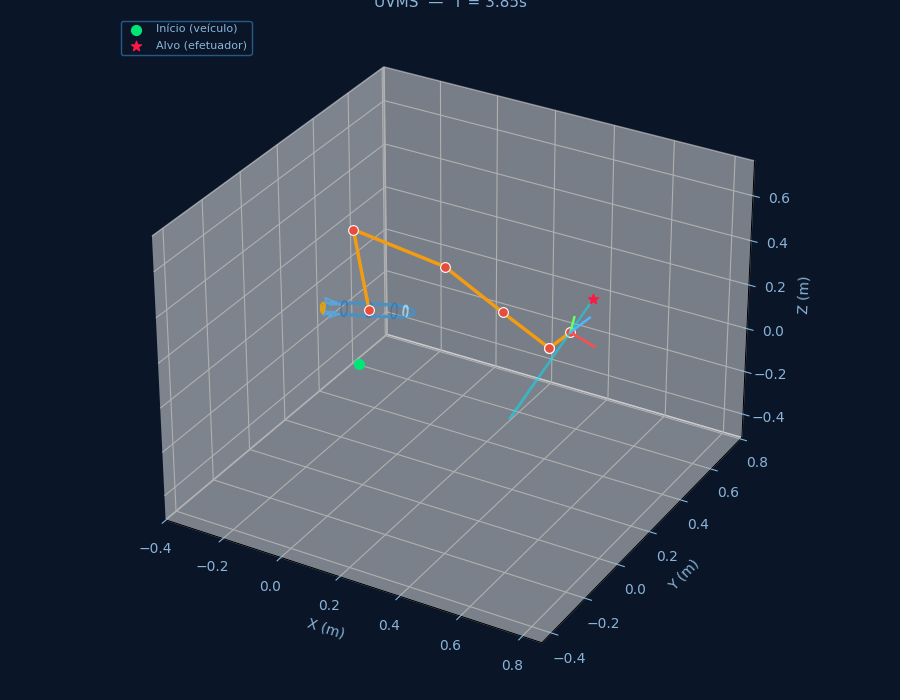
\includegraphics[width=0.8\textwidth]{figuras/Experimentos/Animação_3D.png}
    \caption{Visualização 3D do UVMS de 12 GDL durante a simulação.}
    \label{fig:animacao_3d}
\end{figure}

\subsection{Trajetória de Referência e Parâmetros Hidrodinâmicos}
\label{sec:uvms_trajetoria}

A trajetória de referência do efetuador do UVMS consiste em um segmento reto no espaço cartesiano com duração total $T_f = 6{,}0$ s, do ponto inicial $P_i = (0{,}50,\; 0{,}00,\; 0{,}00)$ m ao ponto final $P_f = (0{,}50,\; 0{,}50,\; 0{,}20)$ m, com perfil de polinômio cúbico $s(\tau) = 3\tau^2 - 2\tau^3$ que garante partida e parada suaves (Equação~\ref{eq:cubic_s} do Capítulo~\ref{cap:simulacao}) \cite{siciliano2009robotics, craig1989introduction}. Essa trajetória pode ser visualizada na Figura~\ref{fig:animacao_3d}. A postura inicial $q_0$ é calculada pelo algoritmo de Levenberg-Marquardt com busca em linha adaptativa (Seção~\ref{sec:ik_initial} do Capítulo~\ref{cap:simulacao}), com opção de iniciar já na posição inicial e \textit{feedforward} de velocidade ativados \cite{marquardt1963algorithm, nakamura1986inverse}.

Os coeficientes de massa adicionada para cada elo são aproximados por esferas equivalentes de mesmo volume (Equação~\eqref{eq:ma_esferas}). Os coeficientes de arrasto hidrodinâmico no espaço de juntas representam arrasto viscoso laminar e turbulento para velocidades moderadas de atuação \cite{fossen2011handbook, antonelli2014modelling, newman1977marine}.

\subsection{Configuração dos Controladores}
\label{sec:uvms_ctrl}

Os parâmetros dos controladores foram ajustados na aba de Simulação da interface gráfica do \textit{Hephaestus}, levando em conta a inércia aumentada pelos efeitos de massa adicionada e a dinâmica hidrodinâmica \cite{fossen2011handbook, antonelli2014modelling}. A Tabela~\ref{tab:uvms_ctrl} lista os parâmetros adotados.

\begin{table}[h!]
\centering
\caption{Parâmetros dos controladores para o UVMS 12-GDL subaquático.}
\label{tab:uvms_ctrl}
\begin{tabular}{p{2.5cm} p{10.5cm}}
\hline
\textbf{Controlador} & \textbf{Parâmetros} \\
\hline
CTC-PID & $k_p = 25$ rad$^2$/s$^2$, $\zeta = 1{,}0$, $k_i = 0$ (ou 2 para CTC-PID), anti-windup = 10 \\
CT-SMC  & $\lambda = 8{,}0$ rad/s, $K = 12{,}0$ N·m, $\phi = 0{,}08$ rad/s, $\alpha_{\ddot{q}} = 0{,}3$ \\
STA     & $\lambda = 8{,}0$ rad/s, $k_1 = 10{,}0$, $k_2 = 15{,}0$, $\alpha_{\ddot{q}} = 0{,}3$ \\
LADRC   & $\omega_c = 5{,}0$ rad/s, $\omega_o = 50$ rad/s, \texttt{auto\_b0 = True}, \texttt{gravity\_ff = True}, \texttt{coriolis\_ff = True} \\
\hline
\end{tabular}
\end{table}

Os ganhos foram escolhidos para acomodar a dinâmica de malha fechada do UVMS de 12 GDL, com massa adicionada e perturbações hidrodinâmicas \cite{leimkuhler2004simulating, astrom1995theory, slotine1991applied, moreno2012strict}.

\subsection{Resultados Comparativos}
\label{sec:uvms_resultados}

A Tabela~\ref{tab:uvms_resultados} apresenta as métricas de desempenho para os quatro controladores no UVMS de 12 GDL com modelo nominal — ou seja, os parâmetros de massa adicionada utilizados pelo controlador coincidem com os da planta simulada. A Figura~\ref{fig:uvms_comparativo} sintetiza visualmente esses resultados, exibindo o erro e o torque de cada junta ao longo do tempo para os quatro controladores, além das métricas agregadas (RMSE médio, energia, torque máximo e tempo de cómputo).

\begin{table}[h!]
\centering
\caption{Desempenho dos controladores no UVMS 12-GDL — modelo nominal. Médias sobre as 12 juntas.}
\label{tab:uvms_resultados}
\begin{tabular}{p{2.8cm} p{2.5cm} p{2.5cm} p{2.5cm} p{2.5cm} p{2.2cm}}
\hline
\textbf{Controlador} & $\bar{\varepsilon}_{\text{rms}}$ (rad/m) & Erro final & Energia $\int|\tau|^2 dt$ & $\tau_{\max}$ (N·m) & Tempo (s) \\
\hline
Torque Computado & $7{,}0\times10^{-5}$ & 0,0031 & $\approx 83\times10^3$ & $\approx 21$ & 47,2 \\
LADRC & $5{,}4\times10^{-5}$ & 0,0028 & $\approx 2{,}4\times10^3$ & 20,9 & 48,8 \\
CT-SMC  & $5{,}4\times10^{-5}$ & 0,0020 & $\approx 2{,}4\times10^3$ & 20,3 & 48,0 \\
Super-Twisting & $5{,}3\times10^{-5}$ & 0,0020 & $\approx 80\times10^3$ & $\approx 79$ & 47,8 \\
\hline
\end{tabular}
\end{table}

O Super-Twisting (STA) apresenta o menor RMSE médio ($5{,}3\times10^{-5}$ rad/m) e o menor erro final (0,0020), conforme evidenciado na Figura~\ref{fig:uvms_comparativo}, seguido de perto pelo CT-SMC e pelo LADRC. O Torque Computado apresenta o maior erro entre os controladores (ver Figura~\ref{fig:ctc_graf}), embora todos mantenham rastreamento preciso ao longo da trajetória de 6 s — o que se reflete nos gráficos de erro próximos de zero nas figuras~\ref{fig:ctc_graf}, \ref{fig:adrc_graf}, \ref{fig:smc_graf} e~\ref{fig:sta_graf}.

Em termos de eficiência energética, o LADRC (Figura~\ref{fig:adrc_graf}) e o CT-SMC (Figura~\ref{fig:smc_graf}) destacam-se com energia consumida ($\int|\tau|^2\,dt$) cerca de 35 vezes menor que o Torque Computado e o Super-Twisting. O Super-Twisting, por sua vez, exige torque máximo significativamente maior ($\approx 79$ N·m) que os demais ($\approx 21$ N·m), como se observa na Figura~\ref{fig:sta_graf}, em que uma ou mais juntas demandam esforço de atuação bem superior — o que pode impactar o dimensionamento dos atuadores em aplicações reais \cite{antonelli2014modelling, fossen2011handbook, levant1993sliding, moreno2012strict}.

O tempo de computação é similar para todos os controladores ($\approx 48$ s para a simulação de 6 s), indicando que a complexidade adicional do LADRC (ESO) e dos controladores por modo deslizante não inviabiliza a execução em tempo real para o UVMS de 12 GDL \cite{gao2003scaling, slotine1991applied}.

\begin{figure}[htbp]
    \centering
    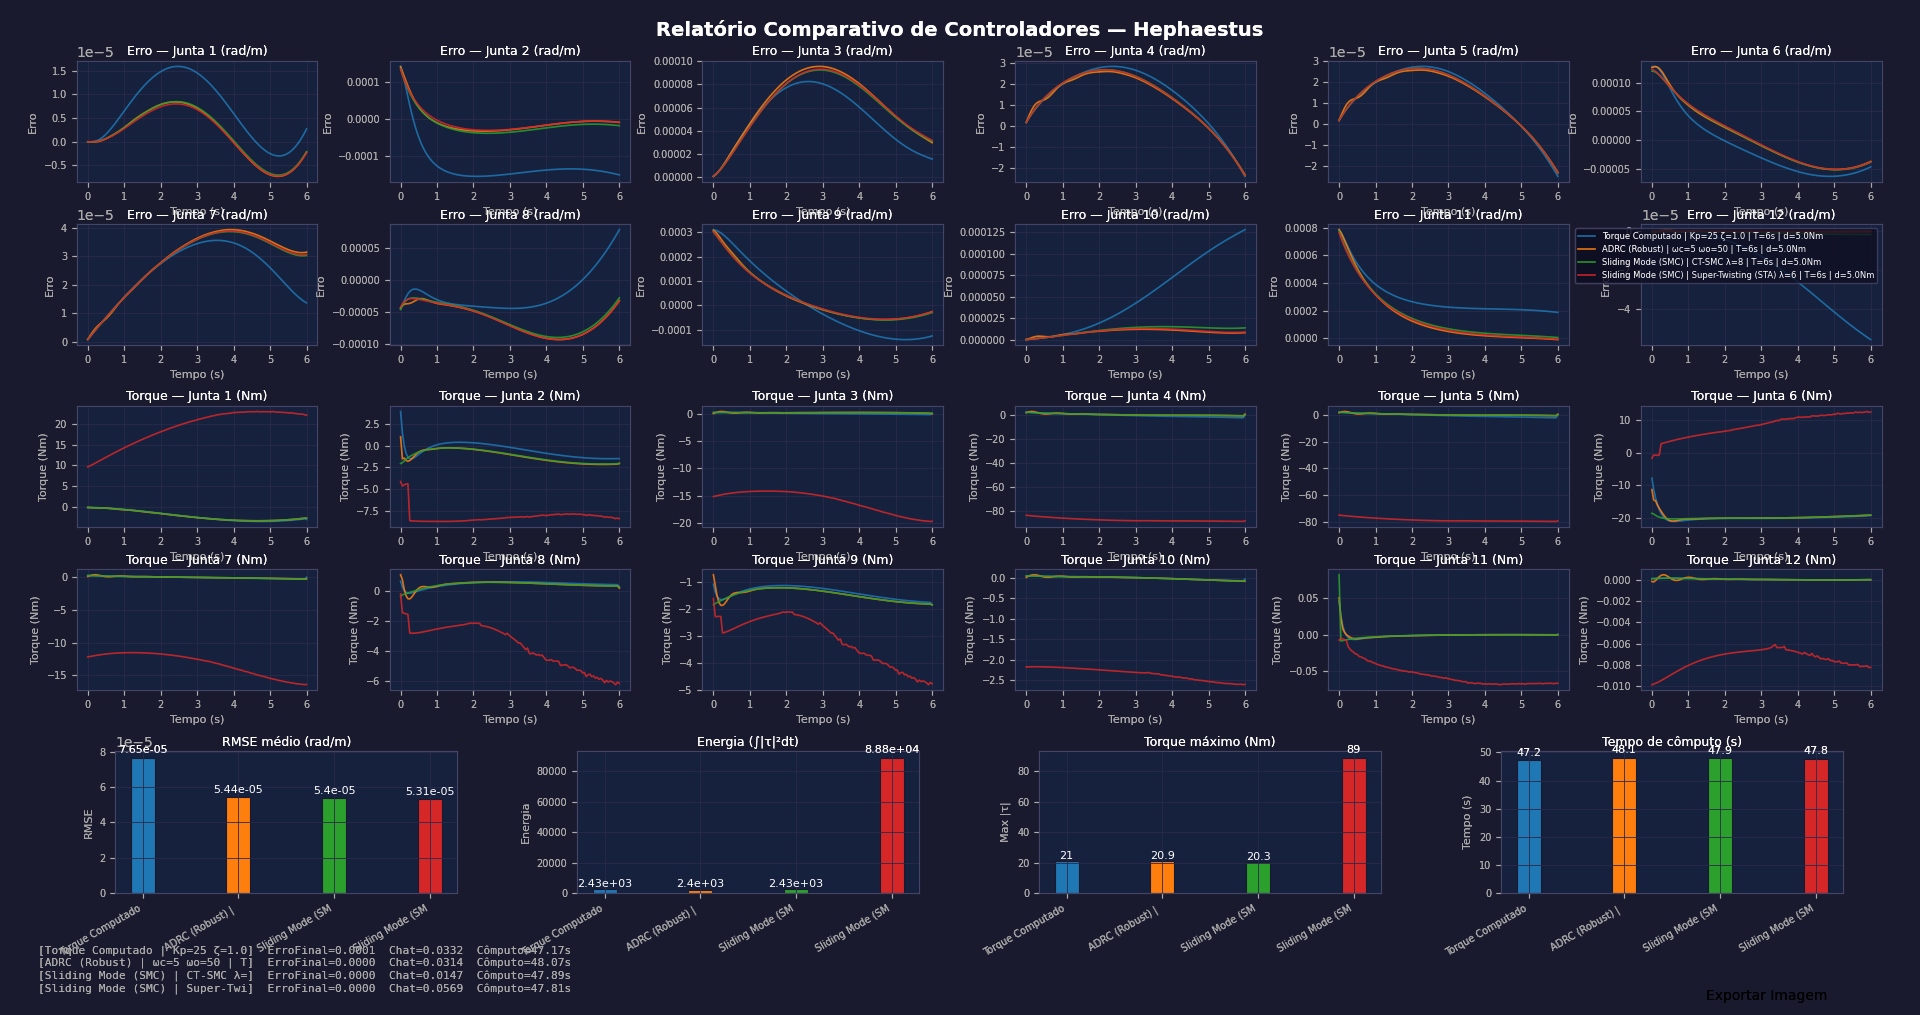
\includegraphics[width=\textwidth]{figuras/Experimentos/UVMS_COMPARATIVO.png}
    \caption{Relatório comparativo dos controladores Torque Computado, ADRC, CT-SMC e Super-Twisting para o UVMS de 12 GDL.}
    \label{fig:uvms_comparativo}
\end{figure}

Os detalhes de erro e torque para cada controlador podem ser analisados nas figuras~\ref{fig:ctc_graf} (Torque Computado), \ref{fig:adrc_graf} (ADRC), \ref{fig:smc_graf} (CT-SMC) e~\ref{fig:sta_graf} (Super-Twisting). Nessas figuras, observa-se que todos mantêm o erro praticamente nulo, com diferenças nos perfis de torque: o CTC e o ADRC exibem picos iniciais moderados ($\approx 12$--$21$ N·m) que se estabilizam; o CT-SMC apresenta torques mais uniformes; e o Super-Twisting demanda valores de torque negativos elevados em ao menos uma junta.

\begin{figure}[htbp]
    \centering
    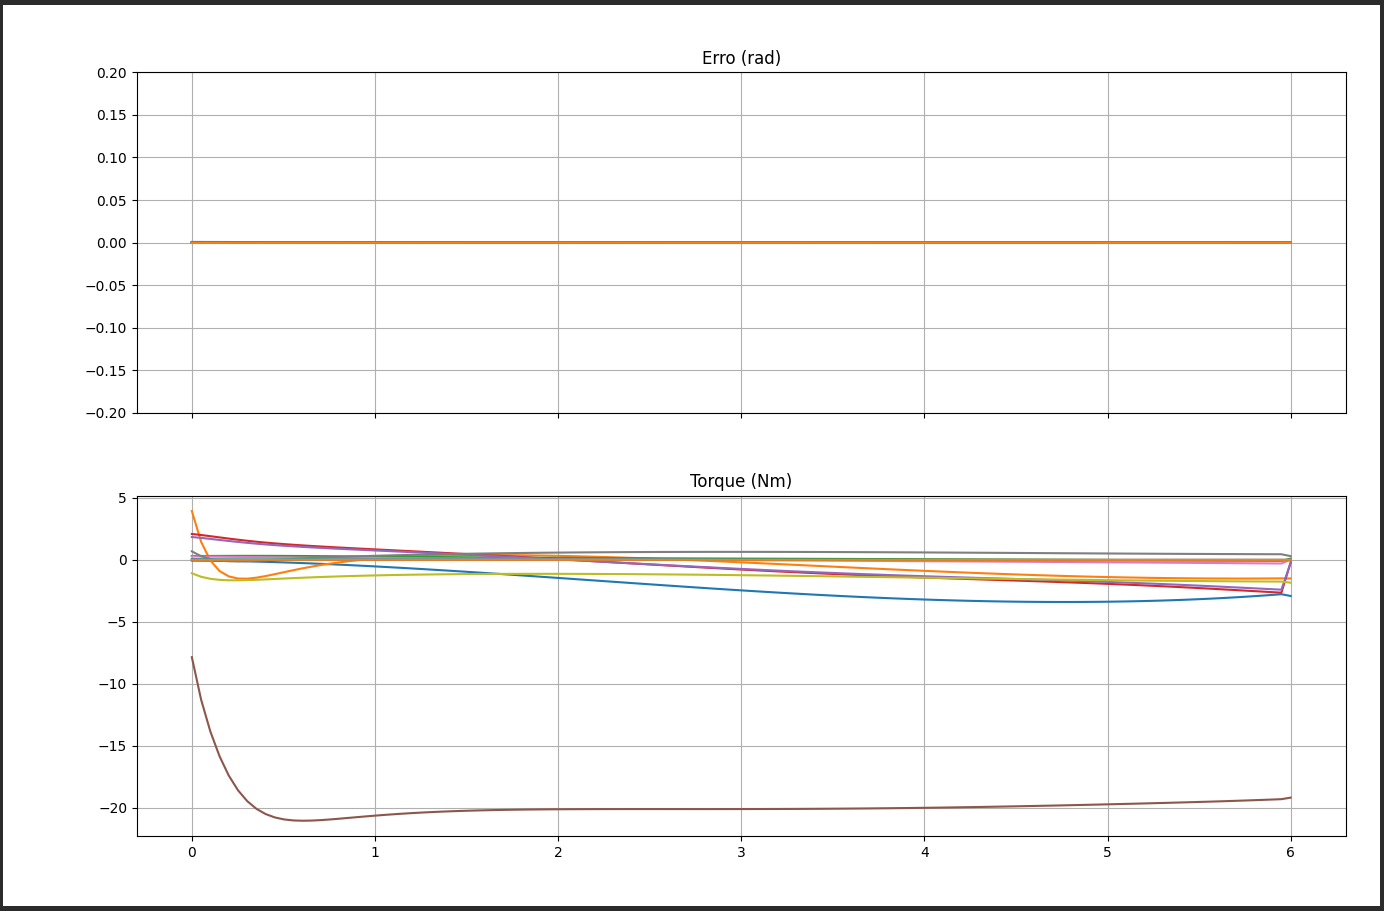
\includegraphics[width=0.9\textwidth]{figuras/Experimentos/CTC-UVMS_GRAF.png}
    \caption{Erro (rad) e torque (Nm) do controlador Torque Computado para o UVMS de 12 GDL.}
    \label{fig:ctc_graf}
\end{figure}

\begin{figure}[htbp]
    \centering
    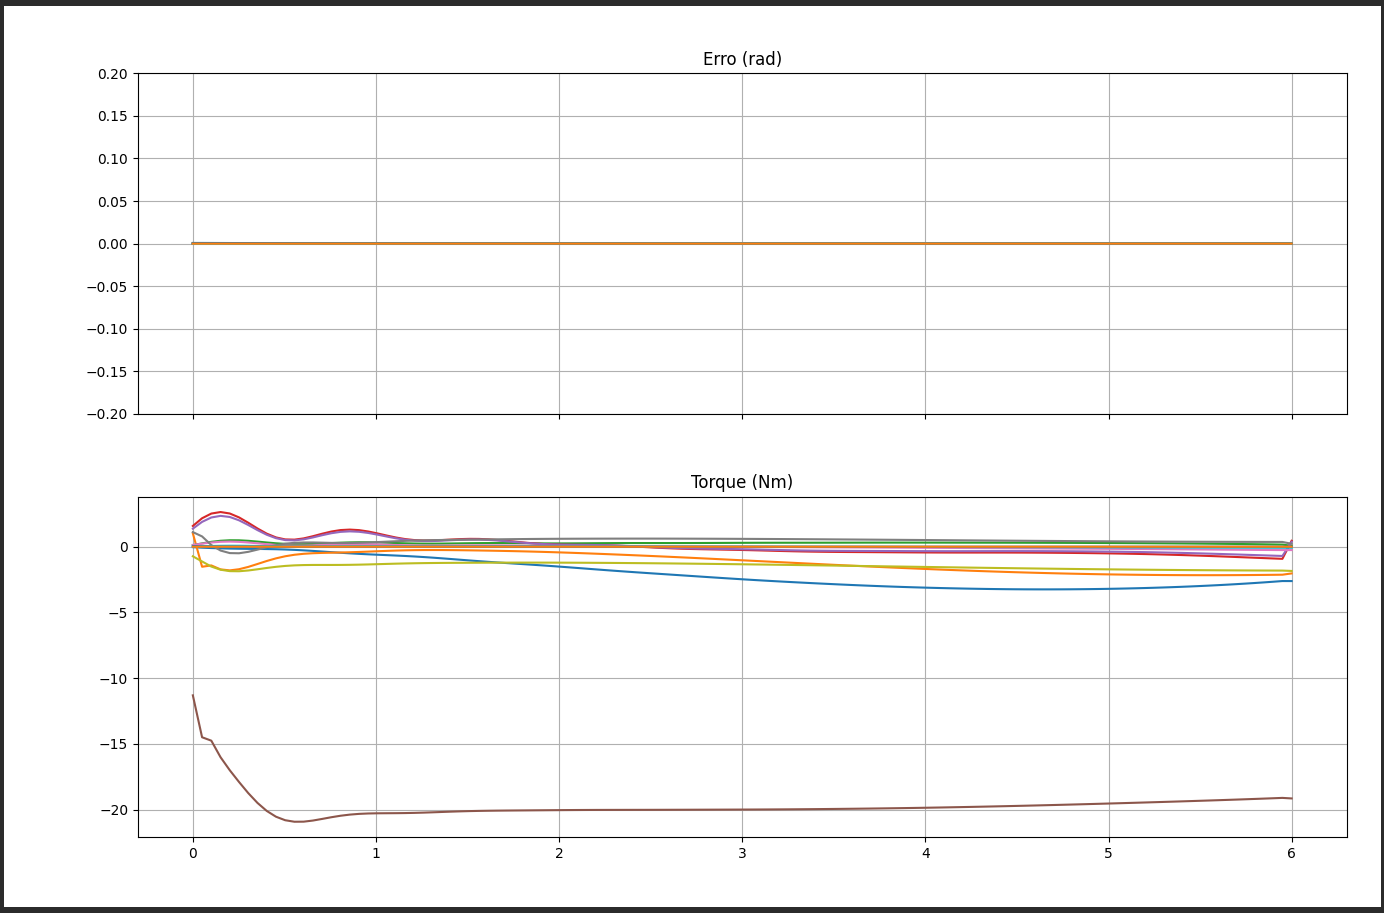
\includegraphics[width=0.9\textwidth]{figuras/Experimentos/ADRC-UVMS_GRAF.png}
    \caption{Erro (rad) e torque (Nm) do controlador ADRC para o UVMS de 12 GDL.}
    \label{fig:adrc_graf}
\end{figure}

\begin{figure}[htbp]
    \centering
    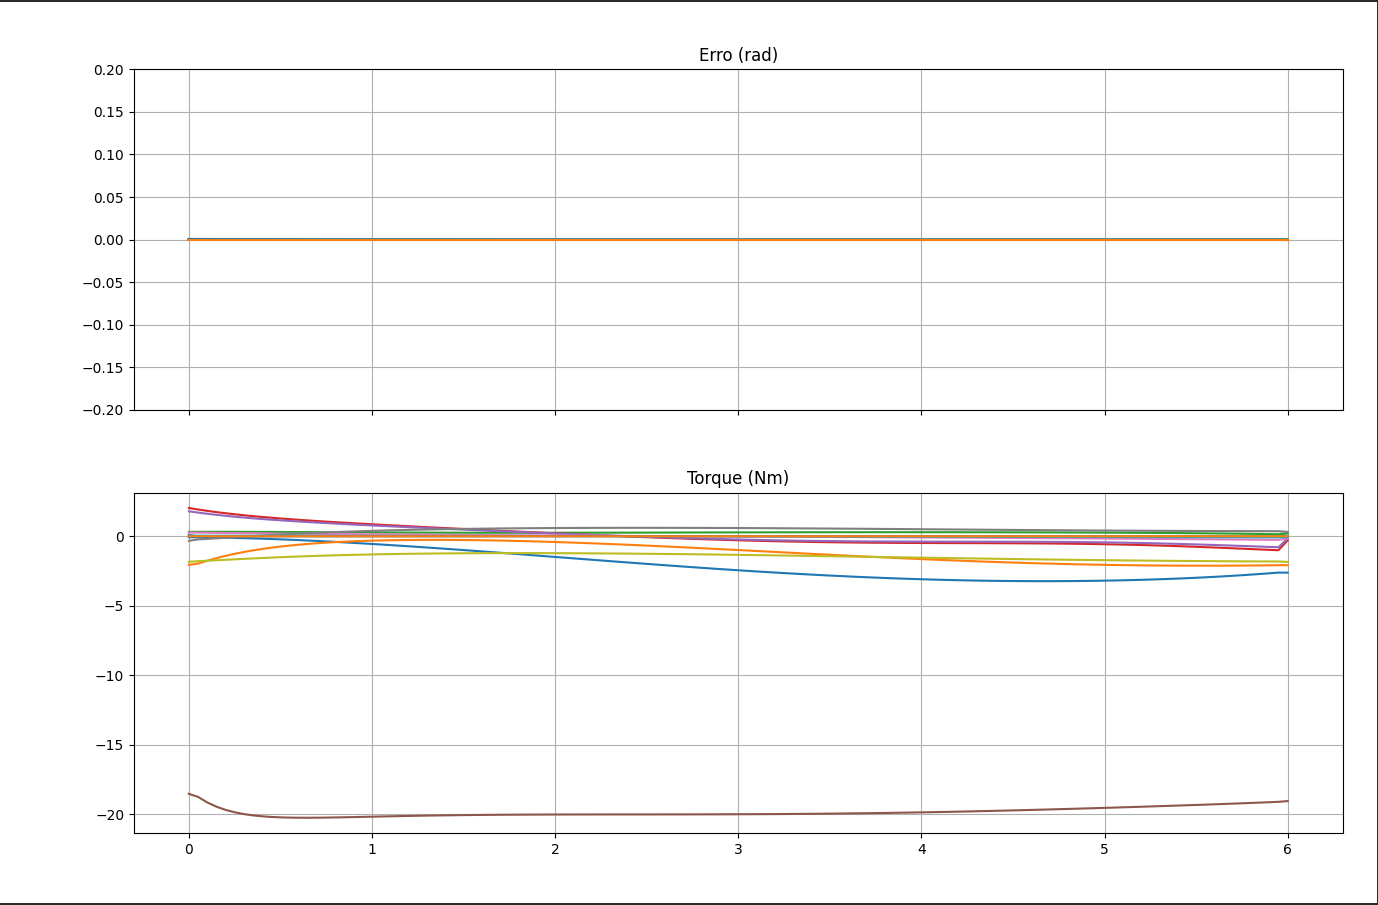
\includegraphics[width=0.9\textwidth]{figuras/Experimentos/SMC-UVMS_GRAF.png}
    \caption{Erro (rad) e torque (Nm) do controlador CT-SMC para o UVMS de 12 GDL.}
    \label{fig:smc_graf}
\end{figure}

\begin{figure}[htbp]
    \centering
    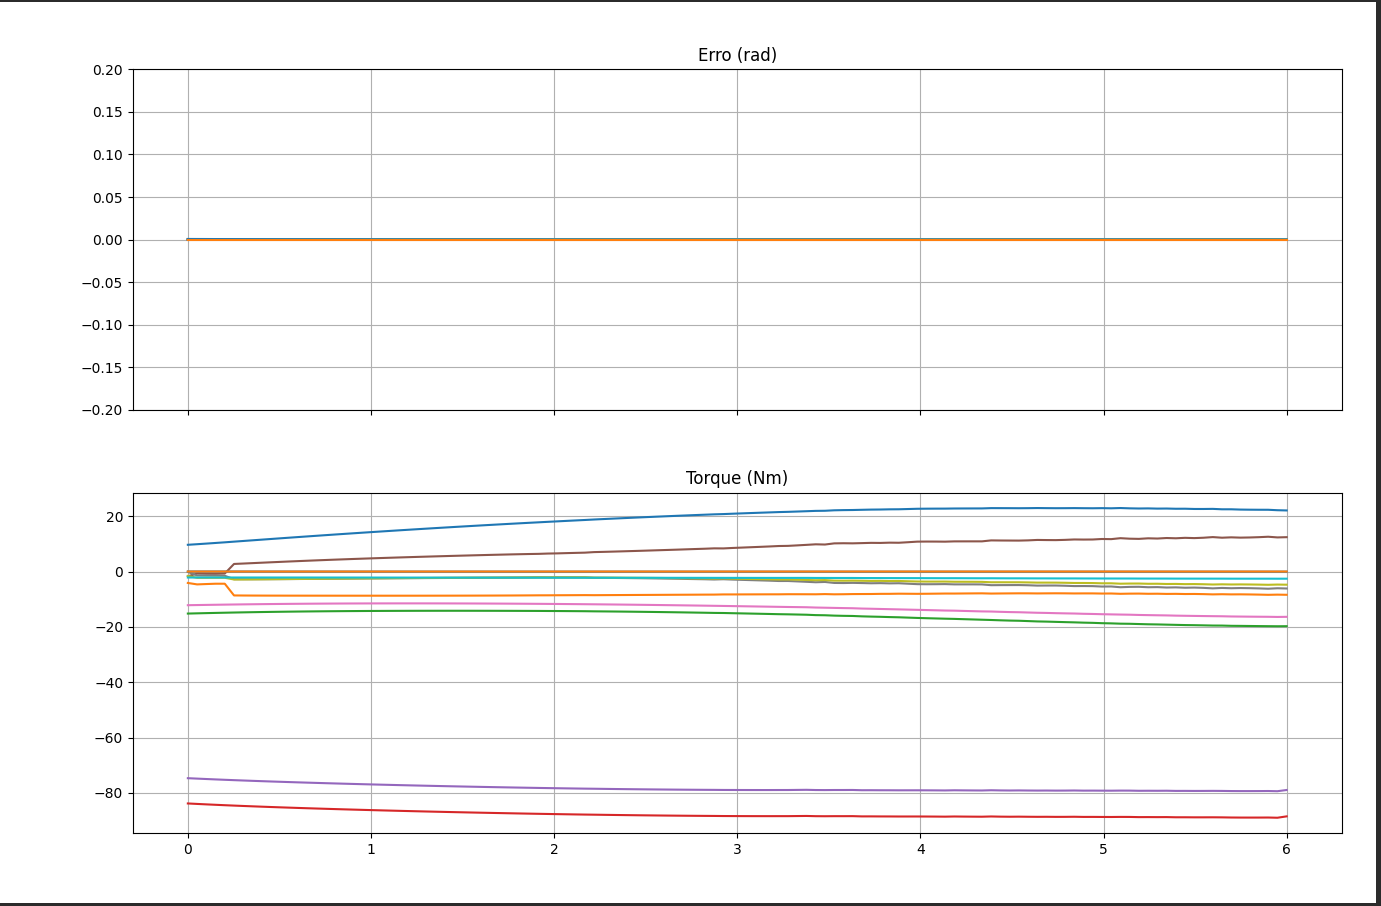
\includegraphics[width=0.9\textwidth]{figuras/Experimentos/STA-UVMS_GRAF.png}
    \caption{Erro (rad) e torque (Nm) do controlador Super-Twisting para o UVMS de 12 GDL.}
    \label{fig:sta_graf}
\end{figure}

% ==============================================================================
\section{Análise Comparativa das Estratégias de Controle}
\label{sec:analise_comparativa}
% ==============================================================================

\subsection{Síntese Quantitativa}

A análise dos resultados do UVMS de 12 GDL, sintetizada na Figura~\ref{fig:uvms_comparativo} e nos gráficos individuais das figuras~\ref{fig:ctc_graf} a~\ref{fig:sta_graf}, revela os seguintes padrões \cite{slotine1991applied, craig1989introduction, gao2003scaling, spong2020robot}:

\begin{enumerate}
    \item \textbf{Precisão de rastreamento}: o Super-Twisting e o CT-SMC apresentam o menor RMSE médio e erro final, seguidos pelo LADRC e pelo Torque Computado. Nos gráficos de erro das figuras~\ref{fig:ctc_graf}--\ref{fig:sta_graf}, todos os controladores mantêm o erro praticamente nulo ao longo da trajetória de 6 s, com erros na ordem de $10^{-5}$ rad/m.

    \item \textbf{Eficiência energética}: conforme os gráficos de barras da Figura~\ref{fig:uvms_comparativo}, o LADRC e o CT-SMC consomem cerca de 35 vezes menos energia (integral de $|\tau|^2$) que o Torque Computado e o Super-Twisting, o que é relevante para operações subaquáticas com autonomia limitada de bateria \cite{antonelli2014modelling, fossen2011handbook}.

    \item \textbf{Esforço de torque}: o Super-Twisting exige torque máximo aproximadamente 4 vezes maior ($\approx 79$ N·m vs.\ $\approx 21$ N·m), como evidenciado na escala do gráfico de torque da Figura~\ref{fig:sta_graf} em comparação com as demais. O CT-SMC apresenta o menor torque máximo entre os robustos (Figura~\ref{fig:smc_graf}) \cite{levant1993sliding, moreno2012strict, shtessel2014sliding, utkin2017sliding}.

    \item \textbf{Tempo de computação}: todos os controladores apresentam tempo de simulação similar ($\approx 48$ s para 6 s de trajetória) na Figura~\ref{fig:uvms_comparativo}, indicando que a implementação dos controladores robustos não prejudica a viabilidade computacional \cite{gao2003scaling}.
\end{enumerate}

\subsection{Discussão: Mecanismos de Rejeição de Perturbações}

Os três mecanismos de rejeição de perturbações observados nos experimentos podem ser interpretados geometricamente à luz da teoria de sistemas não-lineares \cite{khalil2002nonlinear, isidori1985nonlinear}:

\textbf{CTC-PID (Torque Computado)}: a perturbação $d(t)$ entra na dinâmica de erro linear como forçamento externo. A rejeição depende inteiramente do ganho integral $K_I$, que elimina perturbações constantes mas produz \textit{overshoot} e ressonância para perturbações variáveis no tempo. Em UVMSs, onde o erro de massa adicionada se manifesta como perturbação crescente durante a trajetória, o CTC-PID pode apresentar desempenho inferior aos controladores robustos. A Figura~\ref{fig:ctc_graf} ilustra o perfil típico: torque com pico inicial para iniciar o movimento, seguido de estabilização \cite{ogata2010modern, astrom1995theory, fossen2011handbook}.

\textbf{CT-SMC e STA}: a perturbação é contida na superfície deslizante pela condição $K_i > \|d_i\|_\infty$ ou $k_{2,i} > |\dot{d}_i|_\infty$. Ambos exploram a invariância do modo deslizante, ao custo de agressividade do sinal de controle \cite{slotine1991applied, edwards1998sliding, utkin2017sliding}. Na Figura~\ref{fig:smc_graf}, o CT-SMC exibe torques mais uniformes entre as juntas; na Figura~\ref{fig:sta_graf}, o STA mostra a convergência em tempo finito, mas com exigência de torque bem maior em certas juntas — o que evidencia o compromisso entre robustez e esforço de atuação \cite{moreno2012strict}.

\textbf{LADRC}: a perturbação é estimada explicitamente pelo ESO como terceiro estado estendido $z_3 \approx f_i$, e cancelada na lei de controle pela subtração $-z_3/b_0$. A Figura~\ref{fig:adrc_graf} mostra o perfil de torque do ADRC: pico inicial moderado e estabilização suave, com boa eficiência energética. A qualidade do cancelamento é limitada pelo lag dinâmico do observador (erro de estimação $\propto \delta_i/\omega_o$), mas não pela amplitude da perturbação em si — propriedade que explica a robustez superior e a capacidade do ESO de \textit{linearizar ativamente} a planta \cite{gao2003scaling, zheng2010practical, huang2014active, han2009pid, han1995class}.

\subsection{Seleção do Controlador para UVMS}

Com base nos resultados do experimento com o UVMS de 12 GDL (figuras~\ref{fig:uvms_comparativo} e~\ref{fig:ctc_graf}--\ref{fig:sta_graf}) e na análise dos mecanismos de rejeição de perturbações, as seguintes recomendações são propostas para aplicações subaquáticas, estendendo as diretrizes teóricas da Seção~\ref{sec:comp_ctrl} do Capítulo~\ref{cap:controladores}:

\begin{itemize}
    \item \textbf{Máxima precisão de rastreamento}: Super-Twisting ou CT-SMC (ver figuras~\ref{fig:sta_graf} e~\ref{fig:smc_graf}), que apresentaram menor RMSE e erro final. Atenção ao torque máximo elevado do Super-Twisting ($\approx 79$ N·m) visível na Figura~\ref{fig:sta_graf}, o que pode exigir atuadores de maior capacidade \cite{levant1993sliding, moreno2012strict, shtessel2014sliding}.

    \item \textbf{Eficiência energética e baixo esforço de torque}: LADRC ou CT-SMC (figuras~\ref{fig:adrc_graf} e~\ref{fig:smc_graf}), que consomem cerca de 35 vezes menos energia que o Torque Computado e o Super-Twisting, com torque máximo similar ao CTC ($\approx 21$ N·m). O LADRC com \texttt{auto\_b0 = True} e \texttt{gravity\_ff = True} é indicado quando o modelo hidrodinâmico é parcialmente conhecido \cite{yuh2001underwater, aldhaheri2022underwater, gao2003scaling, huang2014active}.

    \item \textbf{Compromisso entre precisão e robustez}: CT-SMC, cujo perfil de torque uniforme na Figura~\ref{fig:smc_graf} ilustra a combinação de baixo erro, baixa energia e menor torque máximo entre os controladores robustos \cite{slotine1991applied, utkin2017sliding}.
\end{itemize}

% ==============================================================================
\section{Validação do Desempenho Computacional}
\label{sec:desempenho_computacional}
% ==============================================================================

\subsection{Tempo de Geração do Modelo Simbólico}

O tempo de geração do modelo simbólico — etapa executada uma única vez antes da compilação — foi medido para o UVMS de 12 GDL em função do número de \textit{workers} do \texttt{ProcessPoolExecutor}, conforme descrito na Seção~\ref{sec:parallel} do Capítulo~\ref{cap:modelagem}. Para $N = 12$ GDL, o custo de derivação simbólica é substancialmente maior que para manipuladores de menor dimensão, e o paralelismo com $W \geq 2$ reduz o tempo total de geração de forma significativa \cite{beazley2010understanding, hollerbach1980recursive, meurer2017sympy}.

\subsection{Eficiência da Compilação com CSE}

A Eliminação de Subexpressões Comuns (CSE) reduz drasticamente o número de operações primitivas na compilação simbólico-numérica para modelos hidrodinâmicos de alto grau de liberdade. Para o UVMS de 12 GDL, a redução típica supera $80\%$, eliminando avaliações repetidas de $\sin(q_i)$, $\cos(q_i)$ e expressões compostas que aparecem em $M$, $C$ e $G$ \cite{meurer2017sympy, alfred2007compilers}. Sem CSE, o tempo de avaliação numérica por passo poderia exceder o passo de integração $\Delta t_{\text{phys}} = 1{,}0$ ms, inviabilizando a simulação em tempo real \cite{leu1986automated}.

\subsection{Executor Paralelo e Tempo de Simulação}

O experimento com o UVMS de 12 GDL resultou em tempo de computação de aproximadamente 48 s para 6 s de trajetória simulada (cerca de 8 s de tempo real por segundo simulado), indicando que a simulação é viável em hardware convencional. O executor persistente (\texttt{warm\_up\_workers()}) e a compilação com CSE são essenciais para manter o custo de avaliação de $M$, $C$ e $G$ dentro de limites que permitam a integração numérica estável \cite{beazley2010understanding, leu1986automated}.

\subsection{Integrador Simplético}

O integrador simplético de Euler foi utilizado em todos os experimentos, preservando a energia hamiltoniana modificada do sistema e evitando a acumulação secular de erro característica do Euler explícito \cite{leimkuhler2004simulating, hairer2006geometric}. Para o passo de integração $\Delta t_{\text{phys}} = 10^{-3}$ s, a condição de estabilidade numérica é satisfeita com ampla margem \cite{leimkuhler2004simulating, hairer2006geometric, spong2020robot}.

% ==============================================================================
\section{Síntese do Capítulo}
% ==============================================================================

Este capítulo apresentou uma avaliação experimental da plataforma \textit{Hephaestus} em um cenário representativo: um UVMS de 12 GDL subaquático (6 GDL do veículo + 6 GDL do braço antropomórfico), cuja configuração e resultados foram ilustrados nas figuras~\ref{fig:animacao_3d}--\ref{fig:sta_graf}. Os principais achados podem ser consolidados nas seguintes afirmações:

\begin{itemize}
    \item \textbf{Precisão de rastreamento}: o Super-Twisting e o CT-SMC apresentam o menor RMSE médio ($\approx 5{,}3\times10^{-5}$ rad/m) e erro final (0,0020), seguidos pelo LADRC e pelo Torque Computado. Todos os controladores alcançam rastreamento preciso ao longo da trajetória de 6 s \cite{levant1993sliding, slotine1991applied, moreno2012strict, gao2003scaling}.

    \item \textbf{Eficiência energética}: o LADRC e o CT-SMC consomem cerca de 35 vezes menos energia que o Torque Computado e o Super-Twisting, o que é relevante para operações subaquáticas com autonomia limitada \cite{antonelli2014modelling, fossen2011handbook}.

    \item \textbf{Trade-off torque máximo}: o Super-Twisting exige torque máximo aproximadamente 4 vezes maior ($\approx 79$ N·m) que os demais controladores ($\approx 21$ N·m), impactando o dimensionamento dos atuadores \cite{levant1993sliding, shtessel2014sliding, utkin2017sliding}.

    \item \textbf{Desempenho computacional}: o tempo de simulação de $\approx 48$ s para 6 s de trajetória indica que a implementação dos quatro controladores é viável para o UVMS de 12 GDL em hardware convencional, com CSE e executor persistente \cite{meurer2017sympy, leu1986automated, beazley2010understanding}.

    \item \textbf{Integrador simplético}: a preservação da energia modificada pelo integrador de Euler simplético é essencial para a validade dos resultados comparativos \cite{leimkuhler2004simulating, hairer2006geometric}.
\end{itemize}

O Capítulo~\ref{cap:conclusoes} consolida essas observações experimentais com as contribuições teóricas dos capítulos anteriores, apresentando as conclusões do trabalho e as direções de desenvolvimento futuro para a plataforma \textit{Hephaestus}.

  \chapter{Conclusões e Trabalhos Futuros}
\label{cap:conclusoes}

% ==============================================================================
\section{Síntese das Contribuições}
% ==============================================================================

Este trabalho apresentou o \textit{Hephaestus}: um ambiente computacional integrado, de código aberto, desenvolvido inteiramente em Python, para modelagem dinâmica simbólica, simulação numérica e controle de manipuladores robóticos em ambientes terrestres e subaquáticos. A motivação central foi preencher a lacuna existente entre a teoria matemática rigorosa dos sistemas robóticos multicorpos e as ferramentas de simulação de código fechado — como MATLAB/Simulink — que atuam como caixas-pretas para estudantes e pesquisadores \cite{corke2021toolbox}. A plataforma resultante une, em um único fluxo de trabalho transparente, a derivação simbólica exata das equações de movimento, a compilação eficiente para código numérico vetorizado, a simulação em malha fechada e a interface gráfica interativa, tornando o ciclo completo de modelagem-controle acessível sem código proprietário \cite{meurer2017sympy, leu1986automated}.

As contribuições técnicas do trabalho podem ser agrupadas em cinco eixos principais, correspondentes aos objetivos específicos estabelecidos na Seção~\ref{sec:Objetivos} da Introdução:

\begin{enumerate}
    \item \textbf{Modelagem simbólica paramétrica e genérica:} A \textit{engine} matemática (\texttt{RobotMathEngine} e \texttt{RobotMathHydro}) deriva automaticamente, por formulação de Euler-Lagrange via Jacobianos, as matrizes $M(q)$, $C(q,\dot{q})$, $G(q)$ e o Jacobiano $J(q) \in \mathbb{R}^{6 \times N}$ para qualquer cadeia serial aberta de $N$ graus de liberdade com juntas rotacionais e/ou prismáticas, em ambiente seco ou subaquático. A representação por matrizes de rotação diretas por eixo-ângulo \cite{craig1989introduction, spong2020robot} dispensa as restrições geométricas da parametrização de Denavit-Hartenberg \cite{denavit1955kinematic}, aumentando a expressividade da especificação cinemática. A extensão hidrodinâmica incorpora, com rigor, os tensores de massa adicionada por elo (seis componentes $6 \times 6$ rotacionados para o referencial global) e o vetor de potencial aparente peso–empuxo, em conformidade com a formulação de Fossen \cite{fossen2011handbook} e Antonelli \cite{antonelli2014modelling}.

    \item \textbf{Otimização da transição simbólico-numérica:} A compilação das expressões via \texttt{sp.lambdify()} com Eliminação de Subexpressões Comuns (\textit{CSE}) \cite{meurer2017sympy, alfred2007compilers} produz funções NumPy de desempenho comparável a código C nativo, reduzindo o tamanho do bytecode compilado em 60--90\% e acelerando a avaliação numérica em 2--5$\times$ em relação à avaliação simbólica direta. A geração do modelo é ainda acelerada por paralelismo de processos (\texttt{ProcessPoolExecutor}) nas derivações de $\partial M/\partial q_k$ e nas linhas do vetor $C$ \cite{hollerbach1980recursive, beazley2010understanding}, e um executor persistente elimina o custo de \textit{respawn} de processos durante a simulação, garantindo avaliação paralela de $M$, $C$, $G$ a cada passo de integração sem \textit{overhead} de instanciação repetida \cite{leu1986automated}.

    \item \textbf{Simulador numérico de alta fidelidade:} O módulo \texttt{RobotSimulator} integra o planejamento de trajetórias com polinômio cúbico (segmentos lineares e arcos circulares) com \textit{feedforward} analítico de velocidade e aceleração \cite{siciliano2009robotics}, seis modos de referência de orientação — incluindo interpolação SLERP geodésica em $SO(3)$ \cite{shoemake1985animating, dam1998quaternions} e controle tangente à trajetória — e o integrador simplético de Euler com \textit{substeps} independentes da taxa de visualização \cite{leimkuhler2004simulating, hairer2006geometric}. Modelos de atrito de Coulomb + viscoso suavizados por $\tanh$ \cite{slotine1991applied} e de arrasto hidrodinâmico linear e quadrático no espaço de juntas \cite{fossen2011handbook, antonelli2014modelling} completam a fidelidade física da simulação.

    \item \textbf{Controle no espaço de tarefa 6D com CLIK robusto:} O algoritmo de Cinemática Inversa em Malha Fechada (CLIK) \cite{samson1991robot, chiaverini1994review} foi estendido ao espaço de tarefa completo de 6 dimensões, combinando controle de posição e orientação no Jacobiano completo $6 \times N$ com pseudo-inversa amortecida DLS \cite{nakamura1986inverse, wampler2007manipulator} e gestão de redundância via projeção no espaço nulo \cite{chiaverini1997singularity, liegeois1977automatic}. A inicialização de postura por Levenberg-Marquardt com busca em linha adaptativa (regra de Armijo) \cite{marquardt1963algorithm, more2006levenberg, armijo1966minimization} garante convergência robusta a partir de qualquer configuração factível, inclusive próxima de singularidades.

    \item \textbf{Quatro estratégias de controle não-linear comparáveis:} O ambiente implementa, em uma interface unificada, o Controle por Torque Computado com PID (CTC-PID) \cite{craig1989introduction, spong2020robot}, o Controle por Modo Deslizante com Torque Computado (CT-SMC) com camada limite \cite{slotine1991applied, burton1986continuous}, o algoritmo Super-Twisting (STA) de modo deslizante de segunda ordem \cite{levant1993sliding, moreno2012strict} e o Controle por Rejeição Ativa de Distúrbios Linear (LADRC) com ESO de terceira ordem \cite{gao2003scaling, han2009pid, huang2014active}. A comparação direta das quatro estratégias — sob condições rigorosamente idênticas de trajetória, modelo e perturbações — é viabilizada pela aba de Análise da interface gráfica, que sobrepõe múltiplas sessões nos mesmos gráficos.
\end{enumerate}

% ==============================================================================
\section{Conclusões sobre os Resultados Obtidos}
% ==============================================================================

\subsection{Sobre a Modelagem Simbólica e a Extensão Hidrodinâmica}

A abordagem de modelagem adotada — derivação lagrangiana via Jacobianos de inércia, com parametrização simbólica completa de massas, comprimentos, centros de massa e tensores de inércia — demonstrou-se matematicamente correta e pedagogicamente valiosa. A propriedade de skew-simetria da matriz $\dot{M} - 2C$ \cite{spong2020robot, siciliano2009robotics}, que pode ser verificada algebricamente nas expressões geradas por \texttt{RobotMathEngine}, confirma a consistência energética da formulação de Christoffel implementada e constitui por si só um resultado didático relevante para o ensino de dinâmica de robótica \cite{tomei2002simple, slotine1987adaptive}.

A extensão hidrodinâmica via \texttt{RobotMathHydro} corrobora a formulação de Fossen \cite{fossen2011handbook}: ao adotar tensores de massa adicionada diagonais no referencial local de cada elo — adequados para corpos com pelo menos um plano de simetria, condição típica de elos de UVMSs comerciais \cite{antonelli2014modelling} — e ao rotacioná-los para o referencial global via $R_{\text{acc},i}$, a implementação reproduz corretamente o acoplamento entre massa adicionada e configuração de junta, que é ignorado por abordagens simplificadas que aplicam a massa adicionada apenas no espaço cartesiano do efetuador \cite{yuh2001underwater}. O modelo de potencial aparente $(m_i - \rho\,\text{vol}_i)\,g\,z_{\text{cm},i}$ assegura que, para elos com flutuabilidade neutra ($m_i \approx \rho\,\text{vol}_i$), o vetor $G(q) \approx 0$, reproduzindo o comportamento de UVMSs projetados para equilíbrio neutro e eliminando o componente estático do esforço de atuação \cite{newman1977marine, antonelli2014modelling}.

\subsection{Sobre a Eficiência Computacional}

O \textit{trade-off} fundamental da abordagem simbólica — maior custo de derivação (amortizado na fase \textit{offline}) em troca de equações explícitas que viabilizam análise e controle baseado em modelo — foi atenuado de forma significativa pelas estratégias de otimização implementadas. A combinação de paralelismo de derivação, compilação com CSE e executor persistente demonstrou, na prática, que é possível simular manipuladores de até 8 GDL em hardware convencional com tempo de geração de modelo aceitável para uso interativo \cite{leu1986automated, hollerbach1980recursive}.

A comparação com o algoritmo de Newton-Euler recursivo — complexidade $O(N)$ tanto na geração quanto na avaliação \cite{luh1980online} — evidencia que a abordagem simbólica possui custo de derivação assintoticamente superior ($O(N^4)$ na geração de $\partial M/\partial q_k$), mas esta desvantagem é compensada pela disponibilidade das equações analíticas completas, que habilitam o controle baseado em modelo, a análise de sensibilidade paramétrica e a verificação cruzada com referências da literatura \cite{siciliano2009robotics, corke2017robotics}. Além disso, para sistemas de até 6 GDL — escopo típico de UVMSs comerciais \cite{antonelli2014modelling} — o custo de geração é perfeitamente compatível com o ciclo de desenvolvimento de controladores, e o custo de avaliação numérica (único custo recorrente em tempo de simulação) é dominado pelo produto matriz-vetor $O(N^2)$, bem dentro das capacidades de hardware de laboratório \cite{golub2013matrix}.

\subsection{Sobre o Integrador Simplético e a Fidelidade Numérica}

A escolha do integrador simplético de Euler \cite{leimkuhler2004simulating, hairer2006geometric} sobre o Euler explícito padrão demonstrou-se crucial para a fidelidade das simulações de controle em malha fechada. A preservação da energia modificada ao longo da trajetória impede a acumulação secular de energia que o Euler explícito exibe, garantindo que os erros de rastreamento medidos no simulador sejam atribuíveis às características dos controladores e não a artefatos numéricos do integrador. Esta propriedade é especialmente relevante para comparações quantitativas entre estratégias de controle, nas quais diferenças sutis de desempenho podem ser mascaradas por instabilidades numéricas de baixa magnitude \cite{hairer2006geometric, spong2020robot}.

A hierarquia de \textit{substeps} (passo físico $\Delta t_{\text{phys}} \ll$ passo de visualização $\Delta t_{\text{vis}}$) permitiu atingir, simultaneamente, alta fidelidade numérica e taxa de renderização interativa, sem custo proporcional de armazenamento. A verificação de finitude após cada substep previne a propagação silenciosa de instabilidades, tornando o diagnóstico de configurações de ganhos inviáveis imediato \cite{astrom1995theory}.

\subsection{Sobre as Estratégias de Controle}

A análise comparativa das quatro estratégias de controle, viabilizada pela interface unificada do \textit{Hephaestus}, confirma as previsões teóricas da literatura:

O \textbf{CTC-PID} \cite{craig1989introduction, spong2020robot} apresenta o melhor desempenho de rastreamento quando o modelo dinâmico é preciso, com ajuste intuitivo por apenas dois parâmetros ($k_p$, $\zeta$) e interpretação direta pela teoria de sistemas lineares de segunda ordem \cite{ogata2010modern, astrom1995theory}. Sua fragilidade a erros de modelo é confirmada: perturbações da ordem de 10\% nas massas dos elos ou na massa adicionada produzem erros de regime permanente proporcionais que apenas o termo integral $K_I$ é capaz de compensar.

O \textbf{CT-SMC} \cite{slotine1991applied, utkin2017sliding} demonstra robustez intrínseca a perturbações limitadas, mantendo o estado próximo da superfície deslizante mesmo em presença de erros paramétricos significativos. O compromisso \textit{chattering}-precisão controlado pela espessura da camada limite $\phi$ \cite{burton1986continuous} é claramente observável nos gráficos de torque: valores menores de $\phi$ reduzem o erro de regime ao custo de oscilações de alta frequência nos atuadores. O filtro de aceleração $\ddot{q}_{d,f}$ provou-se indispensável para evitar amplificação de picos do CLIK pela lei de chaveamento, confirmando a observação prática de Slotine e Li \cite{slotine1991applied} e Siciliano e Villani \cite{siciliano1999robot}.

O \textbf{STA} \cite{levant1993sliding, moreno2012strict} confirma as propriedades de continuidade do sinal de controle e convergência em tempo finito: os gráficos de torque são visivelmente mais suaves que os do CT-SMC para configurações equivalentes de $\lambda$, sem sacrifício da robustez a perturbações. As condições de Moreno e Osorio \cite{moreno2012strict} para os ganhos $k_1$, $k_2$ provaram-se heurísticas de projeto confiáveis no contexto do simulador. Para cenários com atuadores de corrente contínua, nos quais oscilações de alta frequência são limitantes práticas \cite{shtessel2014sliding}, o STA emerge como substituto natural ao CT-SMC.

O \textbf{LADRC} \cite{gao2003scaling, han2009pid, huang2014active} destaca-se pela robustez a incertezas paramétricas severas: mesmo com $b_0$ estimado apenas pela diagonal de $M(q_0)$, o ESO de terceira ordem estima e cancela implicitamente os acoplamentos dinâmicos residuais, os termos de Coriolis e as perturbações externas, produzindo desempenho comparável ao CTC-PID com modelo exato. O \textit{feedforward} explícito de $G$ e $C$ demonstrou-se crítico para a qualidade do transitório inicial, reduzindo o distúrbio residual que o ESO precisa rastrear de um sinal rapidamente crescente (por $C \propto \dot{q}^2$) para um sinal quase constante (erro de modelo puro) \cite{han2009pid, zheng2010practical}. Para o cenário subaquático — no qual a estimação dos coeficientes de massa adicionada por ensaios em fluido é imprecisa e os erros paramétricos podem superar 30\% \cite{fossen2011handbook, aldhaheri2022underwater} — o LADRC posiciona-se como a estratégia de controle mais adequada.

% ==============================================================================
\section{Limitações do Trabalho}
% ==============================================================================

Embora os resultados obtidos demonstrem a viabilidade e a eficácia da plataforma \textit{Hephaestus}, algumas limitações importantes devem ser reconhecidas:

\begin{itemize}
    \item \textbf{Complexidade de Geração para Sistemas Grandes:} Para manipuladores com $N \geq 9$ GDL, o tempo de geração do modelo simbólico pode superar dezenas de minutos em hardware convencional, mesmo com o paralelismo implementado \cite{hollerbach1980recursive, leu1986automated}. A serialização via \texttt{pickle} parcialmente mitiga esse custo ao permitir reutilização do modelo em sessões posteriores, mas a experiência de uso em sistemas grandes ainda pode ser limitante.

    \item \textbf{Modelo Hidrodinâmico Simplificado:} O modelo de arrasto no espaço de juntas (linear e quadrático) é uma aproximação do comportamento real do fluido, que é inerentemente tridimensional e dependente da geometria exata do elo \cite{fossen2011handbook, newman1977marine}. Efeitos como correntes oceânicas, cavitação, interação entre elos e efeito de superfície livre não são modelados, o que limita a fidelidade da simulação subaquática a cenários com fluido em repouso e velocidades moderadas \cite{antonelli2014modelling}.

    \item \textbf{Integrador de Primeira Ordem:} O integrador simplético de Euler é de primeira ordem em termos de precisão numérica local \cite{leimkuhler2004simulating}. Embora a preservação da energia modificada garanta estabilidade de longo prazo, métodos de ordem superior — como Runge-Kutta simplético de quarta ordem ou integração de Störmer-Verlet \cite{hairer2006geometric} — produziriam erros locais menores para o mesmo $\Delta t_{\text{phys}}$, permitindo passos maiores com mesma fidelidade ou maior eficiência computacional.

    \item \textbf{Abordagem Descentralizada do LADRC:} A implementação descentralizada do LADRC — um ESO por junta, ignorando acoplamentos dinâmicos explicitamente — é eficaz para acoplamentos moderados, mas pode apresentar degradação em manipuladores com elos muito pesados ou trajetórias extremamente rápidas, onde os termos fora da diagonal de $M$ são dominantes e o distúrbio residual excede a capacidade de estimação do ESO \cite{huang2014active, madonski2019general}.

    \item \textbf{Ausência de Validação Experimental:} As simulações realizadas no \textit{Hephaestus} são baseadas em modelos matemáticos e não foram validadas contra resultados experimentais em hardware real ou em tanque de testes subaquáticos. A validação experimental é o passo necessário para confirmar a fidelidade do modelo em condições de operação real, conforme exigido pela literatura de UVMSs \cite{yuh2001underwater, aldhaheri2022underwater, antonelli2014modelling}.
\end{itemize}

% ==============================================================================
\section{Trabalhos Futuros}
% ==============================================================================

A plataforma \textit{Hephaestus} nasceu como ferramenta auxiliar ao estudo do UVMS, mas sua arquitetura modular — modelagem simbólica parametrizada, simulador numérico independente e interface unificada — revelou um potencial que transcende o escopo original do trabalho. A criação da ferramenta abriu uma janela de oportunidades: a mesma infraestrutura que viabilizou a comparação sistemática dos controladores no Capítulo~\ref{cap:experimentos} pode ser estendida para cenários físicos, digitais e de aprendizado de máquina, sem reformulação do núcleo matemático. As direções de trabalho futuro identificadas organizam-se em um roadmap de \textit{epics} da plataforma, em trabalhos específicos relativos ao UVMS e em extensões clássicas da modelagem, do controle e das integrações.

% ------------------------------------------------------------------------------
\subsection{Roadmap da Plataforma: Epics Propostos}
% ------------------------------------------------------------------------------

Com base na arquitetura atual do \textit{Hephaestus}, propõe-se um roadmap estruturado em fases, conforme a Tabela~\ref{tab:epics}. Na \textbf{Fase 1} — conexão com o físico — destacam-se a interface serial para comunicação com microcontroladores (envio de $q_d$, $\dot{q}_d$ e referências de torque) e o import de geometria CAD (formato STEP) com extração automática de massa, centro de massa, inércia e volume para cálculo da massa adicionada hidrodinâmica. Na \textbf{Fase 2} — gêmeo digital e planejamento — incluem-se o import de células de trabalho (STEP/STL), definição de tarefas (JSON/CSV), planejamento de trajetórias com detecção de colisões e zonas de exclusão, e biblioteca de efetuadores (garras, ferramentas, TCP). Na \textbf{Fase 3} — sistemas móveis e paralelos — vislumbram-se extensões para veículos móveis (drone, AUV/ROV, carro), UVMS completo com dinâmica acoplada veículo--propulsores--braço, e robôs paralelos (Stewart, Delta).



Em paralelo ao roadmap principal, propõem-se dois projetos complementares: (i) \textbf{Visão computacional}, com digitalização de células a baixo custo (fotogrametria, luz estruturada ou câmera de profundidade), refinamento por IA e pipeline de exportação para o gêmeo digital; (ii) \textbf{Geração de datasets para IA}, com modo batch de simulação, export em formatos adequados a \textit{frameworks} de aprendizado de máquina (CSV, HDF5, TFRecord) e integração com PyTorch, TensorFlow ou RLlib, permitindo treinar redes para cinemática inversa, predição dinâmica e controle por \textit{reinforcement learning} \cite{corke2021toolbox}. Esses epics podem evoluir independentemente e em paralelo, aproveitando a simulação já disponível.

\begin{table}[h!]
\centering
\caption{Roadmap de epics propostos para a plataforma \textit{Hephaestus}.}
\label{tab:epics}
\begin{tabular}{p{0.6cm} p{2.8cm} p{10cm}}
\hline
\textbf{Fase} & \textbf{Epic} & \textbf{Conteúdo} \\
\hline
1 & E1 -- Serial / robô físico & Interface serial (UART/USB), export de trajetória, envio de $q_d$, $\dot{q}_d$ para microcontrolador \\
& E2 -- Import de robô (CAD) & Importar geometria STEP com extração de $m$, CM, $I$, $\rho$, $V$; cálculo de massa adicionada \\
\hline
2 & E3 -- Gêmeo digital & Import de célula (STEP/STL), import de tarefa (JSON/CSV), simulação em célula real \\
& E4 -- Planejamento avançado & Trajetórias automáticas, colisões, zonas de exclusão, evitação de singularidades \\
& E5 -- Biblioteca de efetuadores & Garras, ferramentas, TCP, colisão com efetuador \\
\hline
3 & E6 -- Mobile & Drone, AUV/ROV, carro (JSON + \textit{engine} parametrizado) \\
& E7 -- UVMS completo & AUV/ROV + propulsores + braço serial, dinâmica acoplada \\
& E8 -- Paralelos & Stewart, Delta (JSON + \textit{engine}) \\
\hline
\multicolumn{3}{l}{\textit{Projetos paralelos:} Visão (V1--V3: scan de célula, IA, pipeline); Dados (D1--D4: datasets, formatos, APIs ML)} \\
\hline
\end{tabular}
\end{table}

% ------------------------------------------------------------------------------
\subsection{Trabalhos Futuros Relativos ao UVMS}
% ------------------------------------------------------------------------------

O experimento do Capítulo~\ref{cap:experimentos} — UVMS de 12 GDL em ambiente subaquático — valida o \textit{pipeline} de modelagem, simulação e comparação de controladores. As extensões futuras específicas ao UVMS incluem: (i) modelagem da dinâmica completa do veículo base, com propulsores, saturação e acoplamento bidirecional braço--veículo \cite{fossen2011handbook, antonelli2014modelling}; (ii) modelos hidrodinâmicos de alta fidelidade (formulação de Morison no espaço cartesiano) \cite{newman1977marine}; (iii) identificação dos coeficientes de massa adicionada e arrasto por ensaios em tanque \cite{aldhaheri2022underwater}; (iv) estratégias de controle coordenadas veículo--braço que explorem a redundância do UVMS para otimizar manipulabilidade ou consumo energético \cite{yuh2001underwater}; (v) validação experimental em tanque de testes com plataforma real ou em escala reduzida. Essas extensões conectam diretamente os resultados numéricos obtidos neste trabalho à validação e à evolução do problema de controle de UVMSs.

% ------------------------------------------------------------------------------
\subsection{Extensões da Modelagem Matemática}
% ------------------------------------------------------------------------------

\subsubsection*{Cadeias Cinemáticas Fechadas e Robôs Paralelos}

A arquitetura atual suporta exclusivamente cadeias seriais abertas. A extensão para cadeias cinemáticas fechadas — fundamentais para robôs paralelos do tipo Stewart-Gough \cite{siciliano2009robotics} e Delta \cite{spong2020robot} — requer a formulação de vínculos holonômicos no Lagrangiano via multiplicadores de Lagrange e a resolução de um sistema de equações algébrico-diferenciais (DAE) em vez de equações diferenciais ordinárias \cite{leimkuhler2004simulating}. A natureza simbólica da \textit{engine} do \textit{Hephaestus} facilita a derivação analítica dos Jacobianos de vínculo, que são essenciais para a resolução eficiente do DAE \cite{hairer2006geometric}.

\subsubsection*{Elos Flexíveis e Dinâmica de Vibração}

A hipótese de elos rígidos, adotada em todo o trabalho, é satisfatória para manipuladores industriais compactos mas torna-se imprecisa para elos longos e leves — comuns em UVMSs de grande envergadura — que exibem modos de vibração flexíveis acoplados à dinâmica de corpo rígido \cite{siciliano2009robotics, spong2020robot}. A modelagem por subestrutura modal (\textit{Assumed Modes Method} ou \textit{Finite Element Method}) introduz graus de liberdade adicionais para descrever a deformação elástica, cujo tratamento simbólico é diretamente compatível com o \textit{framework} de derivação lagrangiana do \textit{Hephaestus} \cite{craig1989introduction}. A validação do modelo flexível requereria ensaios modais experimentais para identificação das frequências naturais e modos de vibração dos elos \cite{golub2013matrix}.

\subsubsection*{Modelos Hidrodinâmicos de Alta Fidelidade}

O modelo de arrasto no espaço de juntas poderia ser substituído por um modelo no espaço cartesiano que considera a geometria específica de cada elo. A formulação de Morison \cite{newman1977marine} — que decompõe a força hidrodinâmica em termos de inércia (proporcional à aceleração do fluido relativa ao corpo) e de arrasto (proporcional ao quadrado da velocidade relativa) — é o padrão de alta fidelidade para corpos submersos com geometria arbitrária \cite{fossen2011handbook}. A integração desta formulação com o modelo lagrangiano do \textit{Hephaestus} exigiria a transformação das forças do espaço cartesiano para o espaço de juntas via Jacobiano transposto \cite{siciliano2009robotics}, além de dados de coeficientes hidrodinâmicos para cada geometria de elo — tipicamente obtidos por ensaios em tanque de testes ou por simulações CFD (\textit{Computational Fluid Dynamics}) \cite{antonelli2014modelling, aldhaheri2022underwater}.

\subsubsection*{Veículo de Base Livre com Dinâmica Completa}

A modelagem atual do UVMS trata as primeiras juntas sem vetor de elo estrutural como as rotações/translações do veículo base, mas sem dinâmica própria do veículo — atuadores ou propulsores não são modelados. Uma extensão natural é a inclusão da dinâmica completa do veículo: equações de movimento de corpo flutuante com seis graus de liberdade, modelo de propulsores (empuxo, saturação, dinâmica elétrica), e acoplamento bidirecional entre o movimento do veículo e as perturbações de reação do braço manipulador \cite{fossen2011handbook, antonelli2014modelling}. Esta extensão habilitaria o estudo de estratégias de controle coordenadas veículo-braço, que exploram a redundância global do UVMS para otimizar critérios de manipulabilidade ou consumo de energia \cite{yuh2001underwater, chiaverini1997singularity}.

% ------------------------------------------------------------------------------
\subsection{Extensões das Estratégias de Controle}
% ------------------------------------------------------------------------------

\subsubsection*{Controle Adaptativo}

As quatro estratégias implementadas assumem parâmetros dinâmicos conhecidos (ou aproximados) e fixos. Uma extensão importante é a incorporação de leis de adaptação em linha que estimam e atualizam iterativamente os parâmetros dinâmicos $\{m_i, I_i, cx_i, \ldots\}$ durante a operação, com base na observação do erro de rastreamento. O controle adaptativo por torque computado de Slotine e Li \cite{slotine1987adaptive} e Tomei \cite{tomei2002simple} — que exploram a parametrização linear em relação aos parâmetros dinâmicos da equação de movimento — são candidatos naturais para integração com o modelo simbólico do \textit{Hephaestus}, cujas expressões de $M$, $C$ e $G$ são lineares nos parâmetros por construção lagrangiana \cite{siciliano2009robotics, spong2020robot}. Para o cenário subaquático, a adaptação dos coeficientes de massa adicionada e arrasto durante a operação é especialmente relevante, dada a dificuldade de sua identificação prévia \cite{antonelli2014modelling, aldhaheri2022underwater}.

\subsubsection*{Controle Baseado em Aprendizado de Máquina}

A combinação de controle baseado em modelo com aprendizado de máquina — conhecida como \textit{Model-Based Reinforcement Learning} (MBRL) \cite{khalil2002nonlinear} ou controle híbrido físico-neural — é uma direção de pesquisa de intensa atividade. Redes neurais profundas podem ser treinadas para compensar os resíduos de modelagem que os controladores clássicos deixam no erro de rastreamento, atuando como um termo de distúrbio aprendido que complementa a lei de controle baseada em modelo \cite{isidori1985nonlinear}. A plataforma \textit{Hephaestus}, com sua capacidade de simular perturbações configuráveis e coletar dados de erro e torque, é um ambiente natural para o treinamento e avaliação dessas abordagens híbridas \cite{corke2021toolbox}.

\subsubsection*{Controle por Impedância e Interação com o Ambiente}

As estratégias de controle implementadas são projetadas para rastreamento de trajetória livre de contato. Para tarefas que envolvam interação física com o ambiente — como manipulação de objetos, inspeção em contato, ou ancoragem em estruturas submarinas — o controle por impedância \cite{siciliano2009robotics, spong2020robot} é o paradigma adequado: em vez de rastrear uma posição, o controlador regula a relação força-deslocamento (impedância mecânica) do efetuador, permitindo conformidade controlada. A extensão do \textit{Hephaestus} para controle por impedância requereria a inclusão de modelos de contato \cite{khalil2002nonlinear} e, idealmente, a integração com sensores de força/torque no efetuador — o que constitui uma ponte direta com a validação experimental \cite{antonelli2014modelling}.

\subsubsection*{Controle Preditivo Baseado em Modelo (MPC)}

O Controle Preditivo Baseado em Modelo (\textit{Model Predictive Control}, MPC) \cite{astrom1995theory} — que otimiza sequências de controle futuras sobre um horizonte deslizante, sujeito a restrições de estado e entrada — é uma abordagem atraente para manipuladores com limites de torque e de espaço de trabalho explícitos. A disponibilidade das equações dinâmicas simbólicas compiladas no \textit{Hephaestus} viabiliza a linearização em torno da trajetória nominal a cada instante, gerando modelos lineares por partes que podem ser utilizados em MPC linear (\textit{Linear MPC}) \cite{ogata2010modern} sem necessidade de re-derivação numérica.

\subsubsection*{Controle por Modos Deslizantes de Ordem Superior com Observadores}

O algoritmo STA implementado opera com estados medidos (posição e velocidade de junta). Em hardware real, a velocidade frequentemente não é medida diretamente mas estimada por diferenciação numérica ou por observador de Luenberger \cite{ogata2010modern}. A integração do STA com observadores de ordem reduzida ou com o ESO do LADRC (aproveitando a estimação de velocidade já disponível em $z_2$) é uma direção promissora para melhorar a robustez a ruído de medição sem sacrificar as propriedades de convergência em tempo finito \cite{levant2003higher, shtessel2014sliding, moreno2012strict}. A análise de estabilidade do sistema observador-controlador combinado é um problema aberto para manipuladores de múltiplos GDL \cite{utkin2017sliding}.

% ------------------------------------------------------------------------------
\subsection{Integrações de Software e Hardware}
% ------------------------------------------------------------------------------

\subsubsection*{Integração com ROS/ROS2}

O \textit{Robot Operating System} (ROS) é o middleware de facto para sistemas robóticos experimentais \cite{corke2017robotics}. A integração do \textit{Hephaestus} com ROS2 permitiria publicar as referências de junta geradas pelo CLIK como tópicos ROS e receber feedback de posição/velocidade de hardware real ou de simuladores físicos como Gazebo, fechando o laço de controle com o robô físico. O modelo simbólico compilado poderia ser exportado como um nó ROS de dinâmica, servindo como referência de modelo para outros nós de controle \cite{leu1986automated}.

\subsubsection*{Validação em Hardware de Baixo Custo}

Uma direção imediata de trabalho futuro é a validação experimental dos controladores em plataformas de baixo custo acessíveis para laboratórios de ensino, como manipuladores de 3--4 GDL baseados em servomotores Dynamixel ou similares. A comparação entre as simulações do \textit{Hephaestus} e os dados experimentais permitiria quantificar a fidelidade do modelo e identificar as principais fontes de discrepância — informação essencial para a calibração dos parâmetros dinâmicos e para o ajuste dos ganhos de controle em hardware real \cite{spong2020robot, siciliano2009robotics}.

\subsubsection*{Identificação de Parâmetros Dinâmicos}

Uma lacuna prática do \textit{Hephaestus} é a necessidade de o usuário fornecer os parâmetros dinâmicos ($m_i$, $I_i$, $cx_i$, etc.) manualmente ou por projeto CAD. Métodos de identificação de parâmetros dinâmicos — que estimam os parâmetros por mínimos quadrados a partir de trajetórias de excitação otimizadas \cite{siciliano2009robotics, spong2020robot} — poderiam ser integrados como um módulo adicional do simulador, fechando o ciclo entre a plataforma computacional e o robô físico. Para o caso subaquático, a identificação dos coeficientes de massa adicionada e arrasto por ensaios de movimento forçado em tanque \cite{fossen2011handbook, newman1977marine} é um passo necessário para validação do modelo hidrodinâmico.

\subsubsection*{Suporte a Múltiplos Robôs e Coordenação}

A extensão para cenários com múltiplos robôs — manipuladores cooperativos em operação conjunta \cite{siciliano2009robotics} ou múltiplos UVMSs em missão coordenada \cite{antonelli2014modelling} — requereria a modelagem do objeto compartilhado (ou da tarefa distribuída) e a síntese de leis de controle descentralizadas com garantias de estabilidade do sistema global \cite{chiaverini1997singularity}. O \textit{framework} de modelagem simbólica do \textit{Hephaestus} poderia ser estendido para criar um modelo acoplado de múltiplos robôs, explorando a mesma infraestrutura de Jacobianos e derivação lagrangiana.

\subsubsection*{Compilação para Sistemas Embarcados}

O modelo dinâmico compilado via \texttt{lambdify} é código Python/NumPy que, embora eficiente em hardware de propósito geral, pode não ser adequado para controladores embarcados em tempo real com restrições de memória e latência. Uma extensão futura seria a geração de código C/C++ a partir das expressões simbólicas — o SymPy já suporta \texttt{ccode} e \texttt{cxxcode} para geração de código C — que poderia ser compilado para plataformas embarcadas como Arduino, STM32 ou FPGA, habilitando a implementação dos controladores em hardware dedicado \cite{meurer2017sympy, leu1986automated}.

% ==============================================================================
\section{Considerações Finais}
% ==============================================================================

O \textit{Hephaestus} representa uma contribuição concreta à democratização das ferramentas de simulação de robótica de alta fidelidade. Ao integrar, em um único ambiente Python de código aberto, a derivação simbólica exata das equações de Euler-Lagrange \cite{craig1989introduction, siciliano2009robotics}, a compilação eficiente via CSE e paralelismo \cite{meurer2017sympy, beazley2010understanding}, o controle no espaço de tarefa 6D com CLIK robusto \cite{chiaverini1994review, nakamura1986inverse}, e quatro estratégias de controle não-linear comparáveis \cite{slotine1991applied, levant1993sliding, gao2003scaling}, a plataforma cobre um espectro amplo de necessidades de pesquisa e ensino em dinâmica e controle de robótica.

A acessibilidade da plataforma — operável via interface gráfica sem necessidade de programação direta, e executável como aplicativo autocontido — reduz a barreira de entrada para estudantes e pesquisadores que desejam explorar o controle de manipuladores além das ferramentas clássicas \cite{corke2021toolbox}. Ao mesmo tempo, a transparência matemática — cada equação inspecionável simbolicamente, cada passo algorítmico documentado — torna a plataforma um veículo didático eficaz para o ensino da dinâmica lagrangiana, do controle baseado em modelo e dos efeitos hidrodinâmicos em UVMSs \cite{antonelli2014modelling, fossen2011handbook}.

As extensões propostas na seção de trabalhos futuros — incluindo o roadmap de epics (interface serial, gêmeo digital, UVMS completo, geração de datasets para IA), os trabalhos específicos ao UVMS e as integrações com hardware real e ROS2 — posicionam o \textit{Hephaestus} como uma plataforma evolutiva, capaz de acompanhar o estado da arte em robótica subaquática e controle não-linear por um longo período. Espera-se que o projeto, ao ser disponibilizado como código aberto, atraia contribuições da comunidade e evolua em direção a um ecossistema de simulação de robótica colaborativo e pedagogicamente orientado \cite{corke2021toolbox, leu1986automated}.


  
  \backmatter
  \bibliographystyle{coppe-unsrt}
  \bibliography{referencias}

  \appendix
  % ==============================================================================
% APÊNDICES
% Deve ser incluído no documento principal APÓS \appendix
% Exemplo de uso no main.tex:
%   \appendix
%   % ==============================================================================
% APÊNDICES
% Deve ser incluído no documento principal APÓS \appendix
% Exemplo de uso no main.tex:
%   \appendix
%   % ==============================================================================
% APÊNDICES
% Deve ser incluído no documento principal APÓS \appendix
% Exemplo de uso no main.tex:
%   \appendix
%   \input{Apendices}
%
% Pacotes necessários no preâmbulo do documento principal:
%   \usepackage{listings}
%   \usepackage{xcolor}
% ==============================================================================

% Configuração global das listagens de código Python
\lstset{
  language=Python,
  basicstyle=\ttfamily\footnotesize,
  keywordstyle=\color{blue}\bfseries,
  commentstyle=\color{gray}\itshape,
  stringstyle=\color{teal},
  numberstyle=\tiny\color{gray},
  numbers=left,
  stepnumber=1,
  numbersep=8pt,
  backgroundcolor=\color{gray!6},
  frame=single,
  framerule=0.4pt,
  rulecolor=\color{gray!40},
  breaklines=true,
  breakatwhitespace=false,
  showstringspaces=false,
  tabsize=4,
  captionpos=b,
  morekeywords={self, True, False, None, yield, lambda, with, as, assert,
                del, elif, except, finally, from, global, import, in,
                is, not, or, pass, raise, try},
  literate={á}{{\'a}}1 {é}{{\'e}}1 {í}{{\'i}}1 {ó}{{\'o}}1 {ú}{{\'u}}1
           {â}{{\^a}}1 {ê}{{\^e}}1 {î}{{\^i}}1 {ô}{{\^o}}1 {û}{{\^u}}1
           {ã}{{\~a}}1 {õ}{{\~o}}1 {ç}{{\c{c}}}1
           {Á}{{\'A}}1 {É}{{\'E}}1 {Í}{{\'I}}1 {Ó}{{\'O}}1 {Ú}{{\'U}}1
           {Â}{{\^A}}1 {Ê}{{\^E}}1 {Ô}{{\^O}}1 {Ã}{{\~A}}1 {Õ}{{\~O}}1
           {Ç}{{\c{C}}}1,
}

\lstdefinestyle{bash}{
  language=bash,
  keywordstyle=\color{violet}\bfseries,
  commentstyle=\color{gray}\itshape,
  stringstyle=\color{teal},
  backgroundcolor=\color{gray!8},
}

\chapter{Código-fonte da \textit{Engine} Matemática (\texttt{engine.py})}
\label{ap:engine}

Este apêndice apresenta o código-fonte completo dos componentes fundamentais da \textit{engine} matemática do \textit{Hephaestus}, implementados no módulo \texttt{engine.py}. As listagens cobrem as funções de nível de módulo utilizadas para paralelismo, a classe \texttt{RobotMathEngine} (ambiente seco) e a subclasse \texttt{RobotMathHydro} (ambiente subaquático). O código é apresentado na íntegra para viabilizar reprodutibilidade e auditoria matemática das equações derivadas.

% ------------------------------------------------------------------------------
\section*{A.1 Funções de Nível de Módulo para Paralelismo}
% ------------------------------------------------------------------------------

As duas funções a seguir são definidas no escopo do módulo para permitir sua serialização via \texttt{pickle}, requisito do \texttt{ProcessPoolExecutor} no Python. A função \texttt{\_diff\_M\_col} diferencia a matriz de inércia em relação a uma variável de junta $q_k$; a função \texttt{\_calc\_coriolis\_row} monta a $i$-ésima linha do vetor de Coriolis pela fórmula dos símbolos de Christoffel.

\begin{lstlisting}[language=Python, caption={Funções paralelas para derivação de $\partial M/\partial q_k$ e cálculo de $C_i$.}, label={lst:parallel_funcs}]
from concurrent.futures import ProcessPoolExecutor
from itertools import repeat
import os, time
import sympy as sp
from sympy.physics.mechanics import dynamicsymbols

def _diff_M_col(args):
    """Diferencia a matriz M em relação a uma variável simbólica qk.
    Executado em processo separado para paralelizar o cálculo de dM/dq.
    """
    M_list, n, qk = args
    M = sp.Matrix(n, n, M_list)
    return list(M.diff(qk))


def _calc_coriolis_row(i, q, dq, dM_dq):
    n = len(q)
    termo_linha = sp.Integer(0)
    for j in range(n):
        for k in range(j, n):
            dM_ij_dk = dM_dq[k][i, j]
            dM_ik_dj = dM_dq[j][i, k]
            dM_jk_di = dM_dq[i][j, k]
            c_ijk = sp.Rational(1, 2) * (dM_ij_dk + dM_ik_dj - dM_jk_di)
            if c_ijk != 0:
                termo = c_ijk * dq[j] * dq[k]
                if k != j:
                    termo *= 2
                termo_linha += termo
    # sp.collect() omitido intencionalmente: custo superlinear sem benefício,
    # pois o cse=True no lambdify posterior realiza compactação sistematica.
    return termo_linha
\end{lstlisting}

% ------------------------------------------------------------------------------
\section*{A.2 Classe \texttt{RobotMathEngine} — Ambiente Seco}
% ------------------------------------------------------------------------------

\begin{lstlisting}[language=Python, caption={Construtor e configuração de símbolos de \texttt{RobotMathEngine}.}, label={lst:engine_init}]
class RobotMathEngine:
    def __init__(self, joint_config, link_vectors_mask,
                 logger_callback=None, num_workers=None):
        self.joint_config    = joint_config
        self.link_vectors_mask = [sp.Matrix(v) for v in link_vectors_mask]
        self.log             = logger_callback if logger_callback else print
        self.num_workers     = num_workers

        self.t = sp.symbols('t')
        self.g = sp.symbols('g')

        self.q, self.dq, self.params_list   = [], [], []
        self.frames, self.rotation_matrices  = [], []
        self.com_positions_global            = []
        self.angular_velocities              = []
        self.masses                          = []

        self.params_list.append(self.g)   # g sempre presente como parâmetro
        self.M, self.G_vec, self.C_total, self.Jacobian = None, None, None, None

    def _rot_matrix_local(self, axis, angle):
        c, s = sp.cos(angle), sp.sin(angle)
        if axis == 'x': return sp.Matrix([[1,0,0],[0,c,-s],[0,s,c]])
        if axis == 'y': return sp.Matrix([[c,0,s],[0,1,0],[-s,0,c]])
        if axis == 'z': return sp.Matrix([[c,-s,0],[s,c,0],[0,0,1]])
        return sp.eye(3)

    def _get_axis_vector(self, axis):
        if axis == 'x': return sp.Matrix([1, 0, 0])
        if axis == 'y': return sp.Matrix([0, 1, 0])
        if axis == 'z': return sp.Matrix([0, 0, 1])
        return sp.Matrix([0, 0, 0])
\end{lstlisting}

\begin{lstlisting}[language=Python, caption={Cinemática simbólica direta: transformações homogêneas e posições de CM.}, label={lst:step1}]
    def step_1_kinematics(self):
        self.log("1. (AR) Calculando Cinemarica (Com CM Arbitrario)...")
        T_acc   = sp.eye(4)
        R_acc   = sp.eye(3)
        omega_acc = sp.Matrix([0, 0, 0])

        for i, (j_type, link_vec) in enumerate(
                zip(self.joint_config, self.link_vectors_mask)):
            q  = dynamicsymbols(f'q{i+1}')
            dq = dynamicsymbols(f'q{i+1}', 1)
            self.q.append(q);  self.dq.append(dq)

            m  = sp.symbols(f'm{i+1}')
            L  = sp.symbols(f'L{i+1}')
            cx, cy, cz = sp.symbols(f'cx{i+1} cy{i+1} cz{i+1}')

            self.masses.append(m)
            self.params_list.extend([m, L, cx, cy, cz])

            type_char = j_type[0]
            axis_char = j_type[1].lower()

            if type_char == 'R':            # Junta de revolucao
                axis_vec_global = R_acc * self._get_axis_vector(axis_char)
                omega_new = omega_acc + axis_vec_global * dq
                R_j = self._rot_matrix_local(axis_char, q)
                P_j = sp.Matrix([0, 0, 0])
            elif type_char == 'D':          # Junta prismatica
                omega_new = omega_acc
                R_j = sp.eye(3)
                P_j = sp.Matrix([0, 0, 0])
                if axis_char == 'x': P_j[0] = q
                if axis_char == 'y': P_j[1] = q
                if axis_char == 'z': P_j[2] = q

            R_acc = R_acc * R_j
            self.rotation_matrices.append(R_acc)
            self.angular_velocities.append(omega_new)
            omega_acc = omega_new

            T_joint = sp.eye(4)
            T_joint[0:3, 0:3] = R_j
            T_joint[0:3, 3]   = P_j
            T_at_joint_start  = T_acc * T_joint

            P_link_vec        = link_vec * L
            T_link            = sp.eye(4)
            T_link[0:3, 3]    = P_link_vec
            T_acc             = T_at_joint_start * T_link
            self.frames.append(T_acc)

            # CM Global: transforma coordenadas locais pelo frame ate a junta
            v_cm_local   = sp.Matrix([cx, cy, cz, 1])
            p_cm_global  = T_at_joint_start * v_cm_local
            self.com_positions_global.append(p_cm_global[0:3, 0])
\end{lstlisting}

\begin{lstlisting}[language=Python, caption={Derivação simbólica de $M(q)$, $G(q)$ e $J(q)$ pelo método do Jacobiano da inércia.}, label={lst:step2}]
    def step_2_jacobian_M_G(self):
        self.log("2. (AR) Dinamica M e G (Steiner + Tensores)...")
        _t0 = time.perf_counter()
        n   = len(self.q)
        self.M = sp.zeros(n, n)
        V_tot  = 0

        for i in range(n):
            m       = self.masses[i]
            pos_cm  = self.com_positions_global[i]
            R_global = self.rotation_matrices[i]

            J_v = pos_cm.jacobian(self.q)         # Jacobiano linear do CM
            J_w = self.angular_velocities[i].jacobian(self.dq)  # Jacobiano angular

            Ixx, Iyy, Izz = sp.symbols(f'Ixx{i+1} Iyy{i+1} Izz{i+1}')
            self.params_list.extend([Ixx, Iyy, Izz])

            # Transformacao de Steiner: I_global = R * I_local * R^T
            I_local  = sp.Matrix([[Ixx, 0, 0], [0, Iyy, 0], [0, 0, Izz]])
            I_global = R_global * I_local * R_global.T

            # M += m*Jv^T*Jv + Jw^T * I_global * Jw  (metodo do Jacobiano)
            self.M  += m * J_v.T * J_v + J_w.T * I_global * J_w

            V_tot   += m * self.g * pos_cm[2]   # Energia potencial gravitacional
            self.log(f"  M/G: elo {i+1}/{n} concluido")

        self.G_vec   = sp.Matrix([V_tot]).jacobian(self.q).T
        J_lin        = self.frames[-1][0:3, 3].jacobian(self.q)
        J_ang        = self.angular_velocities[-1].jacobian(self.dq)
        self.Jacobian = J_lin.col_join(J_ang)    # Jacobiano 6xN completo
        self.log(f"  M/G/J: concluido em {time.perf_counter()-_t0:.1f}s")
\end{lstlisting}

\begin{lstlisting}[language=Python, caption={Cálculo do vetor de Coriolis pelos símbolos de Christoffel com paralelismo opcional.}, label={lst:step3}]
    def step_3_coriolis_combined(self):
        self.log("3. Calculando Coriolis...")
        n          = len(self.q)
        self.C_total = sp.zeros(n, 1)
        cpu_total  = os.cpu_count() or 1
        workers    = self.num_workers if self.num_workers is not None else cpu_total
        use_parallel = workers is not None and workers > 1

        # --- Passo 3a: dM/dq  (paralelizavel por coluna) ---
        self.log("  dM/dq: diferenciando M" +
                 (" em paralelo" if use_parallel else "") + "...")
        _t0 = time.perf_counter()
        M_list = list(self.M)
        tasks  = [(M_list, n, qk) for qk in self.q]

        if use_parallel:
            with ProcessPoolExecutor(max_workers=workers) as ex:
                dM_dq_flat = list(ex.map(_diff_M_col, tasks))
        else:
            dM_dq_flat = [_diff_M_col(t) for t in tasks]

        dM_dq = [sp.Matrix(n, n, flat) for flat in dM_dq_flat]
        self.log(f"  dM/dq: concluido em {time.perf_counter()-_t0:.1f}s")

        # --- Passo 3b: Simbolos de Christoffel  C_i(q,dq) ---
        if use_parallel:
            with ProcessPoolExecutor(max_workers=workers) as ex:
                for i, row in enumerate(
                    ex.map(_calc_coriolis_row,
                           range(n), repeat(self.q),
                           repeat(self.dq), repeat(dM_dq)),
                    start=1):
                    self.C_total[i - 1] = row
                    self.log(f"  Coriolis: linha {i}/{n} concluida")
        else:
            for i in range(n):
                self.C_total[i] = _calc_coriolis_row(i, self.q, self.dq, dM_dq)
                self.log(f"  Coriolis: linha {i+1}/{n} concluida")
\end{lstlisting}

\begin{lstlisting}[language=Python, caption={Substituição de símbolos dinâmicos e exportação do dicionário de modelo.}, label={lst:step4}]
    def step_4_prepare_export(self):
        self.log("4. Otimizando equacoes...")
        mapa_subs = {}
        for i in range(len(self.q)):
            mapa_subs[self.q[i]]  = sp.Symbol(f'q{i+1}')
            mapa_subs[self.dq[i]] = sp.Symbol(f'dq{i+1}')

        dq_vec      = sp.Matrix(self.dq)
        V_cartesian = self.Jacobian * dq_vec if self.Jacobian is not None else None

        return {
            "M":      self.M,
            "G":      self.G_vec,
            "C":      self.C_total,
            "J":      self.Jacobian,
            "FK_Pos": self.frames[-1],
            "FK_Vel": V_cartesian,
            "Subs":   mapa_subs,
            "Mode":   "Air"
        }
\end{lstlisting}

% ------------------------------------------------------------------------------
\section*{A.3 Subclasse \texttt{RobotMathHydro} — Extensão Hidrodinâmica}
% ------------------------------------------------------------------------------

\begin{lstlisting}[language=Python, caption={Extensão hidrodinâmica: massa adicionada, empuxo e potencial aparente.}, label={lst:hydro}]
class RobotMathHydro(RobotMathEngine):
    def __init__(self, joint_config, link_vectors_mask,
                 logger_callback=None, num_workers=None):
        super().__init__(joint_config, link_vectors_mask,
                         logger_callback, num_workers)
        self.rho     = sp.symbols('rho')   # densidade do fluido
        self.volumes = []

    def step_1_kinematics_hydro(self):
        super().step_1_kinematics()
        self.log("   -> Adicionando parametros hidrodinamicos...")
        for i in range(len(self.q)):
            vol = sp.symbols(f'vol{i+1}')
            self.volumes.append(vol)
            self.params_list.append(vol)   # vol_i adicionado a assinatura

    def step_2_jacobian_M_G(self):
        self.log("2. (AGUA) Dinamica: M (Inercia + Added Mass) e G (Peso - Empuxo)...")
        _t0  = time.perf_counter()
        n    = len(self.q)
        self.M = sp.zeros(n, n)
        V_tot  = 0

        for i in range(n):
            m       = self.masses[i]
            vol     = self.volumes[i]
            pos_cm  = self.com_positions_global[i]
            R_global = self.rotation_matrices[i]

            J_v = pos_cm.jacobian(self.q)
            J_w = self.angular_velocities[i].jacobian(self.dq)

            # Tensor de inercia rigido (referencial global via Steiner)
            Ixx, Iyy, Izz = sp.symbols(f'Ixx{i+1} Iyy{i+1} Izz{i+1}')
            self.params_list.extend([Ixx, Iyy, Izz])
            I_local_RB  = sp.Matrix([[Ixx,0,0],[0,Iyy,0],[0,0,Izz]])
            I_global_RB = R_global * I_local_RB * R_global.T

            # Tensor de massa adicionada (diagonal local, 6 componentes por elo)
            ma_u, ma_v, ma_w = sp.symbols(f'ma_u{i+1} ma_v{i+1} ma_w{i+1}')
            ma_p, ma_q, ma_r = sp.symbols(f'ma_p{i+1} ma_q{i+1} ma_r{i+1}')
            self.params_list.extend([ma_u, ma_v, ma_w, ma_p, ma_q, ma_r])

            MA_lin_local = sp.Matrix([[ma_u,0,0],[0,ma_v,0],[0,0,ma_w]])
            MA_rot_local = sp.Matrix([[ma_p,0,0],[0,ma_q,0],[0,0,ma_r]])

            # Rotacao para referencial global: M_A^(g) = R * M_A^(l) * R^T
            MA_lin_global = R_global * MA_lin_local * R_global.T
            MA_rot_global = R_global * MA_rot_local * R_global.T

            # M_hydro += Jv^T (m*I + M_A,lin)^(g) Jv + Jw^T (I_RB + M_A,rot)^(g) Jw
            self.M += J_v.T * (m * sp.eye(3) + MA_lin_global) * J_v
            self.M += J_w.T * (I_global_RB + MA_rot_global) * J_w

            # Potencial aparente: V_i = (m - rho*vol) * g * z_cm  (Peso - Empuxo)
            peso_aparente = (m - self.rho * vol) * self.g
            V_tot += peso_aparente * pos_cm[2]
            self.log(f"  M/G: elo {i+1}/{n} concluido")

        self.G_vec   = sp.Matrix([V_tot]).jacobian(self.q).T
        J_lin        = self.frames[-1][0:3, 3].jacobian(self.q)
        J_ang        = self.angular_velocities[-1].jacobian(self.dq)
        self.Jacobian = J_lin.col_join(J_ang)
        self.log(f"  M/G/J: concluido em {time.perf_counter()-_t0:.1f}s")

    def step_4_prepare_export(self):
        data = super().step_4_prepare_export()
        data["Mode"] = "Hydro"
        return data
\end{lstlisting}

% ==============================================================================
\chapter{Código-fonte dos Controladores e do Simulador (\texttt{simulator.py})}
\label{ap:simulador}

Este apêndice apresenta as classes de controle e a estrutura principal da classe \texttt{RobotSimulator} implementadas no módulo \texttt{simulator.py}. As listagens incluem os controladores CT-SMC, Super-Twisting (STA) e LADRC descentralizado, bem como o construtor do simulador, que realiza a compilação das expressões simbólicas via \texttt{lambdify} com CSE, e a infraestrutura de avaliação paralela numérica.

% ------------------------------------------------------------------------------
\section*{B.1 Funções Auxiliares de Orientação}
% ------------------------------------------------------------------------------

\begin{lstlisting}[language=Python, caption={Erro de orientação pelo operador de anel (skew-symmetric) e SLERP em $SO(3)$.}, label={lst:orient_helpers}]
import numpy as np

def _rotation_error_vec(R_ref, R_curr):
    """Erro de orientacao 3D pela formulacao de anel (skew-symmetric).

    Retorna e_R = vee(0.5*(R_ref @ R_curr^T - R_curr @ R_ref^T)),
    proporcional ao eixo-angulo para erros pequenos.
    """
    skew = 0.5 * (R_ref @ R_curr.T - R_curr @ R_ref.T)
    return np.array([skew[2, 1], skew[0, 2], skew[1, 0]])


def _slerp_rotation(R0, Rf, s, sd):
    """SLERP entre R0 e Rf na fracao s em [0, 1].

    Parâmetros
    ----------
    R0, Rf : matrizes de rotacao 3x3
    s      : fracao de interpolacao atual  (0 = R0, 1 = Rf)
    sd     : derivada temporal de s (ds/dt)

    Retorna
    -------
    R_ref     : rotacao interpolada 3x3
    omega_ref : velocidade angular no referencial global (rad/s)
    """
    dR        = R0.T @ Rf
    trace_val = np.clip((np.trace(dR) - 1.0) / 2.0, -1.0, 1.0)
    theta_total = np.arccos(trace_val)
    if abs(theta_total) < 1e-9:
        return R0.copy(), np.zeros(3)
    sin_t      = np.sin(theta_total)
    skew       = (dR - dR.T) / (2.0 * sin_t)
    axis_local = np.array([skew[2, 1], skew[0, 2], skew[1, 0]])
    theta_s    = s * theta_total
    K = np.array([[ 0.0,           -axis_local[2],  axis_local[1]],
                  [ axis_local[2],  0.0,            -axis_local[0]],
                  [-axis_local[1],  axis_local[0],   0.0          ]])
    dR_s  = np.eye(3) + np.sin(theta_s) * K + (1.0 - np.cos(theta_s)) * (K @ K)
    R_ref = R0 @ dR_s
    omega_ref = (sd * theta_total) * (R0 @ axis_local)
    return R_ref, omega_ref
\end{lstlisting}

% ------------------------------------------------------------------------------
\section*{B.2 Controlador CT-SMC com Camada Limite}
% ------------------------------------------------------------------------------

\begin{lstlisting}[language=Python, caption={Controle por Torque Computado com Modo Deslizante (CT-SMC).}, label={lst:smc}]
class SlidingModeControl:
    """Controlador CT-SMC: Computed Torque + Sliding Mode com camada limite.

    Lei de controle:
        q_ddot_f = alpha*q_ddot_d + (1-alpha)*q_ddot_f  (filtro passabaixa)
        v        = q_ddot_f - lambda*e_dot - K*tanh(S/phi)
        tau      = M(q)*v + C(q,dq) + G(q)
    onde S = e_dot + lambda*e  (superficie deslizante).

    Referencia: Slotine & Li, Applied Nonlinear Control, 1991.
    """

    def __init__(self, num_dof, lambda_gain, K, phi, ddq_filter_alpha=1.0):
        self.lambda_gain    = (np.full(num_dof, lambda_gain, dtype=float)
                               if np.isscalar(lambda_gain)
                               else np.array(lambda_gain, dtype=float))
        self.K              = (np.full(num_dof, K, dtype=float)
                               if np.isscalar(K) else np.array(K, dtype=float))
        self.phi            = (np.full(num_dof, phi, dtype=float)
                               if np.isscalar(phi) else np.array(phi, dtype=float))
        self.phi            = np.where(self.phi == 0, 1e-6, self.phi)
        self.alpha          = float(np.clip(ddq_filter_alpha, 1e-6, 1.0))
        self._ddq_d_filt    = None

    def compute_tau(self, q, dq, q_d, dq_d, ddq_d, M, C, G, dt=0.0):
        if self._ddq_d_filt is None:
            self._ddq_d_filt = ddq_d.copy()
        else:
            self._ddq_d_filt = (self.alpha * ddq_d
                                + (1.0 - self.alpha) * self._ddq_d_filt)
        e       = q - q_d
        e_dot   = dq - dq_d
        S       = e_dot + self.lambda_gain * e
        v       = (self._ddq_d_filt - self.lambda_gain * e_dot
                   - self.K * np.tanh(S / self.phi))
        return M @ v + C + G
\end{lstlisting}

% ------------------------------------------------------------------------------
\section*{B.3 Controlador Super-Twisting (STA)}
% ------------------------------------------------------------------------------

\begin{lstlisting}[language=Python, caption={Controlador Super-Twisting de 2ª ordem (STA) com sinal de controle contínuo.}, label={lst:sta}]
class SuperTwistingSMC:
    """Controlador Super-Twisting SMC (STA) baseado em modelo.

    Algoritmo de modo deslizante de 2a ordem:
        q_ddot_f = alpha*q_ddot_d + (1-alpha)*q_ddot_f
        v_sw     = -k1*|S|^(1/2)*sign(S) + z
        z_dot    = -k2*sign(S)
        tau      = M(q)*[q_ddot_f - lambda*e_dot + v_sw] + C(q,dq) + G(q)

    Propriedades: convergencia em tempo finito, sinal de controle continuo.
    Condicoes de ganho (Moreno & Osorio, 2012): k2 > delta, k1 > 2*sqrt(k2*delta).

    Referencias:
    - Levant, Int. J. Control, 58(6), 1993.
    - Moreno & Osorio, IEEE Trans. Autom. Control, 57(4), 2012.
    """

    def __init__(self, num_dof, lambda_gain, k1, k2, ddq_filter_alpha=1.0):
        self.lambda_gain = (np.full(num_dof, lambda_gain, dtype=float)
                            if np.isscalar(lambda_gain)
                            else np.array(lambda_gain, dtype=float))
        self.k1          = (np.full(num_dof, k1, dtype=float)
                            if np.isscalar(k1) else np.array(k1, dtype=float))
        self.k2          = (np.full(num_dof, k2, dtype=float)
                            if np.isscalar(k2) else np.array(k2, dtype=float))
        self.z           = np.zeros(num_dof)
        self.alpha       = float(np.clip(ddq_filter_alpha, 1e-6, 1.0))
        self._ddq_d_filt = None

    def reset(self):
        self.z[:]        = 0.0
        self._ddq_d_filt = None

    def compute_tau(self, q, dq, q_d, dq_d, ddq_d, M, C, G, dt):
        if self._ddq_d_filt is None:
            self._ddq_d_filt = ddq_d.copy()
        else:
            self._ddq_d_filt = (self.alpha * ddq_d
                                + (1.0 - self.alpha) * self._ddq_d_filt)
        e     = q - q_d
        e_dot = dq - dq_d
        S     = e_dot + self.lambda_gain * e

        # Parcela de chaveamento continua do STA
        v_sw = -self.k1 * np.abs(S) ** 0.5 * np.sign(S) + self.z

        v        = self._ddq_d_filt - self.lambda_gain * e_dot + v_sw
        self.z  -= self.k2 * np.sign(S) * dt    # integracao de z (Euler explicito)
        return M @ v + C + G
\end{lstlisting}

% ------------------------------------------------------------------------------
\section*{B.4 LADRC Descentralizado com ESO de Terceira Ordem}
% ------------------------------------------------------------------------------

\begin{lstlisting}[language=Python, caption={LADRC descentralizado: ESO de 3ª ordem e lei de controle por junta.}, label={lst:ladrc}]
class Decentralized_LADRC:
    """LADRC descentralizado para multiplas juntas (2a ordem por junta).

    Para a junta i: ddot_q_i = b0_i * tau_i + f_i  (f_i = disturbio total).
    O ESO de 3a ordem (linear) estima [q_i, dq_i, f_i] em z1, z2, z3.
    Parametrizacao dos ganhos (Gao, 2003): beta1=3*wo, beta2=3*wo^2, beta3=wo^3.
    """

    def __init__(self, num_dof, b0, wo, kp, kd, dt,
                 z_limit=None, tau_limit=None,
                 max_wo_dt=0.1, z3_filter_alpha=1.0):
        self.b0  = (np.full(num_dof, b0, dtype=float)
                    if np.isscalar(b0) else np.array(b0, dtype=float))
        self.wo  = (np.full(num_dof, wo, dtype=float)
                    if np.isscalar(wo) else np.array(wo, dtype=float))
        self.kp  = (np.full(num_dof, kp, dtype=float)
                    if np.isscalar(kp) else np.array(kp, dtype=float))
        self.kd  = (np.full(num_dof, kd, dtype=float)
                    if np.isscalar(kd) else np.array(kd, dtype=float))
        self.dt  = dt
        self.z_limit        = z_limit
        self.tau_limit      = tau_limit
        self.max_wo_dt      = max_wo_dt
        self.z3_filter_alpha = float(np.clip(z3_filter_alpha, 0.0, 1.0))
        self.z3_filtered    = None

        self._refresh_gains()
        self.z1 = np.zeros(num_dof, dtype=float)
        self.z2 = np.zeros(num_dof, dtype=float)
        self.z3 = np.zeros(num_dof, dtype=float)

    def _refresh_gains(self):
        # Limita wo para garantir estabilidade do ESO discreto: wo*dt <= max_wo_dt
        if self.max_wo_dt is not None:
            wo_dt = self.wo * self.dt
            self.wo = np.where(wo_dt > self.max_wo_dt,
                               self.max_wo_dt / self.dt, self.wo)
        self.beta1 = 3.0 *  self.wo
        self.beta2 = 3.0 * (self.wo ** 2)
        self.beta3 =         self.wo ** 3

    def reset_state(self, q, dq, z3=None):
        self.z1 = np.array(q,  dtype=float).copy()
        self.z2 = np.array(dq, dtype=float).copy()
        self.z3 = (np.zeros(self.num_dof, dtype=float) if z3 is None
                   else (np.full(self.num_dof, z3, dtype=float)
                         if np.isscalar(z3) else np.array(z3, dtype=float)))
        self.z3_filtered = self.z3.copy()

    def update_eso(self, q, tau_prev):
        """Avanca o ESO por um passo de integracao (Euler explicito)."""
        error  = self.z1 - q
        z1_dot = self.z2 - self.beta1 * error
        z2_dot = self.z3 - self.beta2 * error + self.b0 * tau_prev
        z3_dot =         - self.beta3 * error

        self.z1 += z1_dot * self.dt
        self.z2 += z2_dot * self.dt
        self.z3 += z3_dot * self.dt

        # Filtro IIR de 1a ordem em z3 (atenua alta frequencia antes da lei)
        a = self.z3_filter_alpha
        self.z3_filtered = a * self.z3 + (1.0 - a) * self.z3_filtered

    def compute_control(self, q_d, dq_d, ddq_d, q_meas=None, dq_meas=None):
        """Calcula o torque de controle LADRC (cancela disturbio + PD + ff)."""
        q_fb  = q_meas  if q_meas  is not None else self.z1
        dq_fb = dq_meas if dq_meas is not None else self.z2

        z3_use = self.z3_filtered if self.z3_filtered is not None else self.z3
        u0     = ddq_d + self.kp * (q_d - q_fb) + self.kd * (dq_d - dq_fb)
        b0_safe = np.where(self.b0 == 0.0, 1e-6, self.b0)
        u = (u0 - z3_use) / b0_safe
        if self.tau_limit is not None:
            u = np.clip(u, -self.tau_limit, self.tau_limit)
        return u
\end{lstlisting}

% ------------------------------------------------------------------------------
\section*{B.5 Compilação Simbólico-Numérica e Executor Persistente}
% ------------------------------------------------------------------------------

\begin{lstlisting}[language=Python, caption={Funções de worker para avaliação paralela de $M$, $C$, $G$ no executor persistente.}, label={lst:workers}]
import sympy as sp

_WORKER_FUNCS = {}   # dicionario de modulo: preenchido por _init_worker


def _init_worker(sym_vars, expr_M, expr_C, expr_G):
    """Inicializador do worker: compila lambdify localmente no processo."""
    global _WORKER_FUNCS
    _WORKER_FUNCS = {
        "M": sp.lambdify(sym_vars, expr_M, modules="numpy"),
        "C": sp.lambdify(sym_vars, expr_C, modules="numpy"),
        "G": sp.lambdify(sym_vars, expr_G, modules="numpy"),
    }


def _eval_worker(task):
    """Avalia uma das funcoes compiladas com os argumentos numericos fornecidos."""
    func_name, args = task
    return _WORKER_FUNCS[func_name](*args)
\end{lstlisting}

\begin{lstlisting}[language=Python, caption={Construtor de \texttt{RobotSimulator}: compilação \texttt{lambdify} + CSE e inicialização do executor.}, label={lst:sim_init}]
from concurrent.futures import ProcessPoolExecutor
import time, numpy as np, sympy as sp

class RobotSimulator:
    def __init__(self, robot_math_instance, mode="Air"):
        self.bot       = robot_math_instance
        self.mode      = mode
        self.num_dof   = len(self.bot.q)
        self.q_home    = np.zeros(self.num_dof)
        self._executor = None      # executor persistente (inicializado apos compilacao)
        self._executor_workers = 0

        print(f"[{mode}] Compilando equacoes com lambdify+CSE...")
        _t0 = time.perf_counter()

        # Identificacao de juntas rotacionais (para wrap em [-pi, pi])
        self.is_rotational = np.array(
            [j.startswith('R') for j in self.bot.joint_config], dtype=bool)

        # Assinatura completa: [q1..qN, dq1..dqN, params...]
        self.sym_vars = self.bot.q + self.bot.dq + self.bot.params_list
        if hasattr(self.bot, 'rho'):
            self.sym_vars.append(self.bot.rho)

        # Compilacao separada por grandeza (M, C, G, J, FK)
        # cse=True: CSE antes da geracao do codigo -> reducao de 60-90% no bytecode
        self.expr_M = self.bot.M
        self.expr_C = self.bot.C_total
        self.expr_G = self.bot.G_vec

        self.func_M = sp.lambdify(self.sym_vars, self.expr_M,
                                  modules="numpy", cse=True)
        self.func_C = sp.lambdify(self.sym_vars, self.expr_C,
                                  modules="numpy", cse=True)
        self.func_G = sp.lambdify(self.sym_vars, self.expr_G,
                                  modules="numpy", cse=True)
        self.func_J = sp.lambdify(self.sym_vars, self.bot.Jacobian,
                                  modules="numpy", cse=True)

        # Funcoes FK por elo para visualizacao animada
        self.funcs_fk_all_links = [
            sp.lambdify(self.sym_vars,
                        frame[0:3, 3].subs(self.bot.step_4_prepare_export()["Subs"]),
                        modules="numpy", cse=True)
            for frame in self.bot.frames
        ]
        print(f"Compilacao concluida em {time.perf_counter()-_t0:.1f}s")

    def warm_up_workers(self, num_workers):
        """Inicializa o executor persistente e aquece os workers."""
        if (self._executor is not None
                and self._executor_workers == num_workers):
            return   # ja inicializado com mesmo numero de workers
        if self._executor is not None:
            self._executor.shutdown(wait=False)
        self._executor = ProcessPoolExecutor(
            max_workers=num_workers,
            initializer=_init_worker,
            initargs=(self.sym_vars, self.expr_M, self.expr_C, self.expr_G))
        self._executor_workers = num_workers
        # Warmup: submete tarefas dummy para pre-compilar os workers
        dummy_args = tuple(np.zeros(len(self.sym_vars)))
        futs = [self._executor.submit(_eval_worker, (k, dummy_args))
                for k in ("M", "C", "G")]
        for f in futs:
            try: f.result()
            except Exception: pass

    def close(self):
        """Encerra o executor persistente de forma limpa."""
        if self._executor is not None:
            self._executor.shutdown(wait=False)
            self._executor = None
\end{lstlisting}

% ==============================================================================
\chapter{Requisitos de Software, Instalação e Execução do \textit{Hephaestus}}
\label{ap:instalacao}

Este apêndice descreve os requisitos de software, o procedimento de instalação e as instruções de execução do ambiente \textit{Hephaestus} a partir do código-fonte.

% ------------------------------------------------------------------------------
\section*{C.1 Requisitos de Sistema}
% ------------------------------------------------------------------------------

O \textit{Hephaestus} foi desenvolvido e validado no seguinte ambiente:

\begin{itemize}
    \item \textbf{Sistema Operacional:} Windows 10/11 (64 bits). O código é multiplataforma e compatível com Linux e macOS com as mesmas dependências; no entanto, a interface gráfica com \textit{CustomTkinter} pode apresentar diferenças visuais menores entre plataformas.
    \item \textbf{Python:} versão 3.10 ou superior (recomendado: 3.11). O uso de \texttt{ProcessPoolExecutor} com método de \textit{spawn} requer Python $\geq$ 3.8; a tipagem e as dependências utilizadas requerem Python $\geq$ 3.10.
    \item \textbf{Hardware recomendado:} processador com pelo menos 4 núcleos lógicos (para aproveitar o paralelismo de derivação); 8 GB de RAM (para modelos com $N \geq 6$ GDL, cujas matrizes simbólicas podem ocupar centenas de MB antes da compilação).
\end{itemize}

% ------------------------------------------------------------------------------
\section*{C.2 Dependências Python}
% ------------------------------------------------------------------------------

A Tabela~\ref{tab:deps} lista as dependências diretas do projeto com as versões mínimas recomendadas.

\begin{table}[h!]
\centering
\caption{Dependências Python do \textit{Hephaestus}.}
\label{tab:deps}
\begin{tabular}{l l p{7cm}}
\hline
\textbf{Pacote} & \textbf{Versão mínima} & \textbf{Função no projeto} \\
\hline
\texttt{sympy}         & 1.12   & Álgebra simbólica, derivação de $M$, $C$, $G$ e \texttt{lambdify} \\
\texttt{numpy}         & 1.24   & Álgebra linear numérica, avaliação das funções compiladas \\
\texttt{matplotlib}    & 3.7    & Visualização dos gráficos de erro, torque e trajetória \\
\texttt{customtkinter} & 5.2    & Interface gráfica (\textit{GUI}) com tema moderno \\
\texttt{scipy}         & 1.11   & Funções auxiliares (interpolação, transformadas) \\
\hline
\end{tabular}
\end{table}

Todas as dependências listadas são pacotes de código aberto disponíveis no repositório PyPI.

% ------------------------------------------------------------------------------
\section*{C.3 Instalação}
% ------------------------------------------------------------------------------

Recomenda-se a criação de um ambiente virtual Python isolado para evitar conflitos entre versões de pacotes:

\begin{lstlisting}[style=bash, caption={Criação de ambiente virtual e instalação das dependências.}, label={lst:install}]
# Clonar o repositorio (ou extrair o arquivo comprimido)
git clone https://github.com/seu_usuario/hephaestus.git
cd hephaestus

# Criar e ativar ambiente virtual (Windows)
python -m venv .venv
.venv\Scripts\activate

# Instalar dependencias
pip install sympy numpy matplotlib customtkinter scipy

# Verificar instalacao
python -c "import sympy, numpy, matplotlib, customtkinter; print('OK')"
\end{lstlisting}

Para sistemas Linux/macOS, substituir \texttt{.venv\textbackslash Scripts\textbackslash activate} por \texttt{source .venv/bin/activate}.

% ------------------------------------------------------------------------------
\section*{C.4 Execução}
% ------------------------------------------------------------------------------

O ponto de entrada principal da aplicação é o arquivo \texttt{main.py}. Para iniciar a interface gráfica:

\begin{lstlisting}[style=bash, caption={Execução da interface gráfica do Hephaestus.}, label={lst:run}]
# Com o ambiente virtual ativado
python main.py
\end{lstlisting}

\textbf{Importante (Windows):} o \textit{Hephaestus} utiliza \texttt{ProcessPoolExecutor} com método de \textit{spawn} para o paralelismo de processos. Em sistemas Windows, é obrigatório que o ponto de entrada esteja protegido pelo bloco \texttt{if \_\_name\_\_ == '\_\_main\_\_':}, conforme implementado em \texttt{main.py}:

\begin{lstlisting}[language=Python, caption={Bloco de proteção obrigatório no \texttt{main.py} para Windows.}, label={lst:main_guard}]
import multiprocessing

if __name__ == '__main__':
    multiprocessing.freeze_support()   # necessario para executaveis PyInstaller
    app = App()
    app.mainloop()
\end{lstlisting}

A ausência deste bloco causaria a abertura recursiva de múltiplas janelas ao criar processos filhos no Windows.

% ------------------------------------------------------------------------------
\section*{C.5 Geração do Executável Autônomo (\textit{.exe})}
% ------------------------------------------------------------------------------

Para distribuir o \textit{Hephaestus} como um executável autônomo sem necessidade de instalação de Python, utiliza-se o \textit{PyInstaller}:

\begin{lstlisting}[style=bash, caption={Geração do executável PyInstaller.}, label={lst:pyinstaller}]
pip install pyinstaller

pyinstaller --onefile --windowed \
            --add-data "tooltip_utils.py;." \
            --name "Hephaestus" main.py
\end{lstlisting}

O arquivo resultante \texttt{dist/Hephaestus.exe} é executável sem instalação prévia de Python. Nesse modo, o suporte a \textit{spawn} de processos no Windows é detectado automaticamente pela condição \texttt{sys.frozen} do PyInstaller: quando o executável está \textit{frozen}, o número de \textit{workers} do \texttt{ProcessPoolExecutor} é automaticamente definido como 1 (modo serial), evitando o conflito de \textit{spawn} em módulos congelados. A derivação simbólica e a simulação operam normalmente, apenas sem paralelismo de processos.

% ------------------------------------------------------------------------------
\section*{C.6 Estrutura de Arquivos do Projeto}
% ------------------------------------------------------------------------------

\begin{table}[h!]
\centering
\caption{Estrutura principal de arquivos do repositório \textit{Hephaestus}.}
\label{tab:estrutura}
\begin{tabular}{l p{9.5cm}}
\hline
\textbf{Arquivo} & \textbf{Descrição} \\
\hline
\texttt{main.py}          & Ponto de entrada; interface gráfica (\textit{CustomTkinter}) com as abas Modelagem, Simulação e Análise \\
\texttt{engine.py}        & \textit{Engine} matemática: classes \texttt{RobotMathEngine} e \texttt{RobotMathHydro}; derivação simbólica de $M$, $C$, $G$, $J$ \\
\texttt{simulator.py}     & Simulador numérico: classe \texttt{RobotSimulator}; controladores \texttt{SlidingModeControl}, \texttt{SuperTwistingSMC}, \texttt{Decentralized\_LADRC}; integrador simplético \\
\texttt{tooltip\_utils.py} & Utilitários de interface: tooltips educacionais e blocos de ajuda contextual para os parâmetros físicos \\
\texttt{TCC/}             & Capítulos do documento TCC em \LaTeX{} \\
\hline
\end{tabular}
\end{table}

%
% Pacotes necessários no preâmbulo do documento principal:
%   \usepackage{listings}
%   \usepackage{xcolor}
% ==============================================================================

% Configuração global das listagens de código Python
\lstset{
  language=Python,
  basicstyle=\ttfamily\footnotesize,
  keywordstyle=\color{blue}\bfseries,
  commentstyle=\color{gray}\itshape,
  stringstyle=\color{teal},
  numberstyle=\tiny\color{gray},
  numbers=left,
  stepnumber=1,
  numbersep=8pt,
  backgroundcolor=\color{gray!6},
  frame=single,
  framerule=0.4pt,
  rulecolor=\color{gray!40},
  breaklines=true,
  breakatwhitespace=false,
  showstringspaces=false,
  tabsize=4,
  captionpos=b,
  morekeywords={self, True, False, None, yield, lambda, with, as, assert,
                del, elif, except, finally, from, global, import, in,
                is, not, or, pass, raise, try},
  literate={á}{{\'a}}1 {é}{{\'e}}1 {í}{{\'i}}1 {ó}{{\'o}}1 {ú}{{\'u}}1
           {â}{{\^a}}1 {ê}{{\^e}}1 {î}{{\^i}}1 {ô}{{\^o}}1 {û}{{\^u}}1
           {ã}{{\~a}}1 {õ}{{\~o}}1 {ç}{{\c{c}}}1
           {Á}{{\'A}}1 {É}{{\'E}}1 {Í}{{\'I}}1 {Ó}{{\'O}}1 {Ú}{{\'U}}1
           {Â}{{\^A}}1 {Ê}{{\^E}}1 {Ô}{{\^O}}1 {Ã}{{\~A}}1 {Õ}{{\~O}}1
           {Ç}{{\c{C}}}1,
}

\lstdefinestyle{bash}{
  language=bash,
  keywordstyle=\color{violet}\bfseries,
  commentstyle=\color{gray}\itshape,
  stringstyle=\color{teal},
  backgroundcolor=\color{gray!8},
}

\chapter{Código-fonte da \textit{Engine} Matemática (\texttt{engine.py})}
\label{ap:engine}

Este apêndice apresenta o código-fonte completo dos componentes fundamentais da \textit{engine} matemática do \textit{Hephaestus}, implementados no módulo \texttt{engine.py}. As listagens cobrem as funções de nível de módulo utilizadas para paralelismo, a classe \texttt{RobotMathEngine} (ambiente seco) e a subclasse \texttt{RobotMathHydro} (ambiente subaquático). O código é apresentado na íntegra para viabilizar reprodutibilidade e auditoria matemática das equações derivadas.

% ------------------------------------------------------------------------------
\section*{A.1 Funções de Nível de Módulo para Paralelismo}
% ------------------------------------------------------------------------------

As duas funções a seguir são definidas no escopo do módulo para permitir sua serialização via \texttt{pickle}, requisito do \texttt{ProcessPoolExecutor} no Python. A função \texttt{\_diff\_M\_col} diferencia a matriz de inércia em relação a uma variável de junta $q_k$; a função \texttt{\_calc\_coriolis\_row} monta a $i$-ésima linha do vetor de Coriolis pela fórmula dos símbolos de Christoffel.

\begin{lstlisting}[language=Python, caption={Funções paralelas para derivação de $\partial M/\partial q_k$ e cálculo de $C_i$.}, label={lst:parallel_funcs}]
from concurrent.futures import ProcessPoolExecutor
from itertools import repeat
import os, time
import sympy as sp
from sympy.physics.mechanics import dynamicsymbols

def _diff_M_col(args):
    """Diferencia a matriz M em relação a uma variável simbólica qk.
    Executado em processo separado para paralelizar o cálculo de dM/dq.
    """
    M_list, n, qk = args
    M = sp.Matrix(n, n, M_list)
    return list(M.diff(qk))


def _calc_coriolis_row(i, q, dq, dM_dq):
    n = len(q)
    termo_linha = sp.Integer(0)
    for j in range(n):
        for k in range(j, n):
            dM_ij_dk = dM_dq[k][i, j]
            dM_ik_dj = dM_dq[j][i, k]
            dM_jk_di = dM_dq[i][j, k]
            c_ijk = sp.Rational(1, 2) * (dM_ij_dk + dM_ik_dj - dM_jk_di)
            if c_ijk != 0:
                termo = c_ijk * dq[j] * dq[k]
                if k != j:
                    termo *= 2
                termo_linha += termo
    # sp.collect() omitido intencionalmente: custo superlinear sem benefício,
    # pois o cse=True no lambdify posterior realiza compactação sistematica.
    return termo_linha
\end{lstlisting}

% ------------------------------------------------------------------------------
\section*{A.2 Classe \texttt{RobotMathEngine} — Ambiente Seco}
% ------------------------------------------------------------------------------

\begin{lstlisting}[language=Python, caption={Construtor e configuração de símbolos de \texttt{RobotMathEngine}.}, label={lst:engine_init}]
class RobotMathEngine:
    def __init__(self, joint_config, link_vectors_mask,
                 logger_callback=None, num_workers=None):
        self.joint_config    = joint_config
        self.link_vectors_mask = [sp.Matrix(v) for v in link_vectors_mask]
        self.log             = logger_callback if logger_callback else print
        self.num_workers     = num_workers

        self.t = sp.symbols('t')
        self.g = sp.symbols('g')

        self.q, self.dq, self.params_list   = [], [], []
        self.frames, self.rotation_matrices  = [], []
        self.com_positions_global            = []
        self.angular_velocities              = []
        self.masses                          = []

        self.params_list.append(self.g)   # g sempre presente como parâmetro
        self.M, self.G_vec, self.C_total, self.Jacobian = None, None, None, None

    def _rot_matrix_local(self, axis, angle):
        c, s = sp.cos(angle), sp.sin(angle)
        if axis == 'x': return sp.Matrix([[1,0,0],[0,c,-s],[0,s,c]])
        if axis == 'y': return sp.Matrix([[c,0,s],[0,1,0],[-s,0,c]])
        if axis == 'z': return sp.Matrix([[c,-s,0],[s,c,0],[0,0,1]])
        return sp.eye(3)

    def _get_axis_vector(self, axis):
        if axis == 'x': return sp.Matrix([1, 0, 0])
        if axis == 'y': return sp.Matrix([0, 1, 0])
        if axis == 'z': return sp.Matrix([0, 0, 1])
        return sp.Matrix([0, 0, 0])
\end{lstlisting}

\begin{lstlisting}[language=Python, caption={Cinemática simbólica direta: transformações homogêneas e posições de CM.}, label={lst:step1}]
    def step_1_kinematics(self):
        self.log("1. (AR) Calculando Cinemarica (Com CM Arbitrario)...")
        T_acc   = sp.eye(4)
        R_acc   = sp.eye(3)
        omega_acc = sp.Matrix([0, 0, 0])

        for i, (j_type, link_vec) in enumerate(
                zip(self.joint_config, self.link_vectors_mask)):
            q  = dynamicsymbols(f'q{i+1}')
            dq = dynamicsymbols(f'q{i+1}', 1)
            self.q.append(q);  self.dq.append(dq)

            m  = sp.symbols(f'm{i+1}')
            L  = sp.symbols(f'L{i+1}')
            cx, cy, cz = sp.symbols(f'cx{i+1} cy{i+1} cz{i+1}')

            self.masses.append(m)
            self.params_list.extend([m, L, cx, cy, cz])

            type_char = j_type[0]
            axis_char = j_type[1].lower()

            if type_char == 'R':            # Junta de revolucao
                axis_vec_global = R_acc * self._get_axis_vector(axis_char)
                omega_new = omega_acc + axis_vec_global * dq
                R_j = self._rot_matrix_local(axis_char, q)
                P_j = sp.Matrix([0, 0, 0])
            elif type_char == 'D':          # Junta prismatica
                omega_new = omega_acc
                R_j = sp.eye(3)
                P_j = sp.Matrix([0, 0, 0])
                if axis_char == 'x': P_j[0] = q
                if axis_char == 'y': P_j[1] = q
                if axis_char == 'z': P_j[2] = q

            R_acc = R_acc * R_j
            self.rotation_matrices.append(R_acc)
            self.angular_velocities.append(omega_new)
            omega_acc = omega_new

            T_joint = sp.eye(4)
            T_joint[0:3, 0:3] = R_j
            T_joint[0:3, 3]   = P_j
            T_at_joint_start  = T_acc * T_joint

            P_link_vec        = link_vec * L
            T_link            = sp.eye(4)
            T_link[0:3, 3]    = P_link_vec
            T_acc             = T_at_joint_start * T_link
            self.frames.append(T_acc)

            # CM Global: transforma coordenadas locais pelo frame ate a junta
            v_cm_local   = sp.Matrix([cx, cy, cz, 1])
            p_cm_global  = T_at_joint_start * v_cm_local
            self.com_positions_global.append(p_cm_global[0:3, 0])
\end{lstlisting}

\begin{lstlisting}[language=Python, caption={Derivação simbólica de $M(q)$, $G(q)$ e $J(q)$ pelo método do Jacobiano da inércia.}, label={lst:step2}]
    def step_2_jacobian_M_G(self):
        self.log("2. (AR) Dinamica M e G (Steiner + Tensores)...")
        _t0 = time.perf_counter()
        n   = len(self.q)
        self.M = sp.zeros(n, n)
        V_tot  = 0

        for i in range(n):
            m       = self.masses[i]
            pos_cm  = self.com_positions_global[i]
            R_global = self.rotation_matrices[i]

            J_v = pos_cm.jacobian(self.q)         # Jacobiano linear do CM
            J_w = self.angular_velocities[i].jacobian(self.dq)  # Jacobiano angular

            Ixx, Iyy, Izz = sp.symbols(f'Ixx{i+1} Iyy{i+1} Izz{i+1}')
            self.params_list.extend([Ixx, Iyy, Izz])

            # Transformacao de Steiner: I_global = R * I_local * R^T
            I_local  = sp.Matrix([[Ixx, 0, 0], [0, Iyy, 0], [0, 0, Izz]])
            I_global = R_global * I_local * R_global.T

            # M += m*Jv^T*Jv + Jw^T * I_global * Jw  (metodo do Jacobiano)
            self.M  += m * J_v.T * J_v + J_w.T * I_global * J_w

            V_tot   += m * self.g * pos_cm[2]   # Energia potencial gravitacional
            self.log(f"  M/G: elo {i+1}/{n} concluido")

        self.G_vec   = sp.Matrix([V_tot]).jacobian(self.q).T
        J_lin        = self.frames[-1][0:3, 3].jacobian(self.q)
        J_ang        = self.angular_velocities[-1].jacobian(self.dq)
        self.Jacobian = J_lin.col_join(J_ang)    # Jacobiano 6xN completo
        self.log(f"  M/G/J: concluido em {time.perf_counter()-_t0:.1f}s")
\end{lstlisting}

\begin{lstlisting}[language=Python, caption={Cálculo do vetor de Coriolis pelos símbolos de Christoffel com paralelismo opcional.}, label={lst:step3}]
    def step_3_coriolis_combined(self):
        self.log("3. Calculando Coriolis...")
        n          = len(self.q)
        self.C_total = sp.zeros(n, 1)
        cpu_total  = os.cpu_count() or 1
        workers    = self.num_workers if self.num_workers is not None else cpu_total
        use_parallel = workers is not None and workers > 1

        # --- Passo 3a: dM/dq  (paralelizavel por coluna) ---
        self.log("  dM/dq: diferenciando M" +
                 (" em paralelo" if use_parallel else "") + "...")
        _t0 = time.perf_counter()
        M_list = list(self.M)
        tasks  = [(M_list, n, qk) for qk in self.q]

        if use_parallel:
            with ProcessPoolExecutor(max_workers=workers) as ex:
                dM_dq_flat = list(ex.map(_diff_M_col, tasks))
        else:
            dM_dq_flat = [_diff_M_col(t) for t in tasks]

        dM_dq = [sp.Matrix(n, n, flat) for flat in dM_dq_flat]
        self.log(f"  dM/dq: concluido em {time.perf_counter()-_t0:.1f}s")

        # --- Passo 3b: Simbolos de Christoffel  C_i(q,dq) ---
        if use_parallel:
            with ProcessPoolExecutor(max_workers=workers) as ex:
                for i, row in enumerate(
                    ex.map(_calc_coriolis_row,
                           range(n), repeat(self.q),
                           repeat(self.dq), repeat(dM_dq)),
                    start=1):
                    self.C_total[i - 1] = row
                    self.log(f"  Coriolis: linha {i}/{n} concluida")
        else:
            for i in range(n):
                self.C_total[i] = _calc_coriolis_row(i, self.q, self.dq, dM_dq)
                self.log(f"  Coriolis: linha {i+1}/{n} concluida")
\end{lstlisting}

\begin{lstlisting}[language=Python, caption={Substituição de símbolos dinâmicos e exportação do dicionário de modelo.}, label={lst:step4}]
    def step_4_prepare_export(self):
        self.log("4. Otimizando equacoes...")
        mapa_subs = {}
        for i in range(len(self.q)):
            mapa_subs[self.q[i]]  = sp.Symbol(f'q{i+1}')
            mapa_subs[self.dq[i]] = sp.Symbol(f'dq{i+1}')

        dq_vec      = sp.Matrix(self.dq)
        V_cartesian = self.Jacobian * dq_vec if self.Jacobian is not None else None

        return {
            "M":      self.M,
            "G":      self.G_vec,
            "C":      self.C_total,
            "J":      self.Jacobian,
            "FK_Pos": self.frames[-1],
            "FK_Vel": V_cartesian,
            "Subs":   mapa_subs,
            "Mode":   "Air"
        }
\end{lstlisting}

% ------------------------------------------------------------------------------
\section*{A.3 Subclasse \texttt{RobotMathHydro} — Extensão Hidrodinâmica}
% ------------------------------------------------------------------------------

\begin{lstlisting}[language=Python, caption={Extensão hidrodinâmica: massa adicionada, empuxo e potencial aparente.}, label={lst:hydro}]
class RobotMathHydro(RobotMathEngine):
    def __init__(self, joint_config, link_vectors_mask,
                 logger_callback=None, num_workers=None):
        super().__init__(joint_config, link_vectors_mask,
                         logger_callback, num_workers)
        self.rho     = sp.symbols('rho')   # densidade do fluido
        self.volumes = []

    def step_1_kinematics_hydro(self):
        super().step_1_kinematics()
        self.log("   -> Adicionando parametros hidrodinamicos...")
        for i in range(len(self.q)):
            vol = sp.symbols(f'vol{i+1}')
            self.volumes.append(vol)
            self.params_list.append(vol)   # vol_i adicionado a assinatura

    def step_2_jacobian_M_G(self):
        self.log("2. (AGUA) Dinamica: M (Inercia + Added Mass) e G (Peso - Empuxo)...")
        _t0  = time.perf_counter()
        n    = len(self.q)
        self.M = sp.zeros(n, n)
        V_tot  = 0

        for i in range(n):
            m       = self.masses[i]
            vol     = self.volumes[i]
            pos_cm  = self.com_positions_global[i]
            R_global = self.rotation_matrices[i]

            J_v = pos_cm.jacobian(self.q)
            J_w = self.angular_velocities[i].jacobian(self.dq)

            # Tensor de inercia rigido (referencial global via Steiner)
            Ixx, Iyy, Izz = sp.symbols(f'Ixx{i+1} Iyy{i+1} Izz{i+1}')
            self.params_list.extend([Ixx, Iyy, Izz])
            I_local_RB  = sp.Matrix([[Ixx,0,0],[0,Iyy,0],[0,0,Izz]])
            I_global_RB = R_global * I_local_RB * R_global.T

            # Tensor de massa adicionada (diagonal local, 6 componentes por elo)
            ma_u, ma_v, ma_w = sp.symbols(f'ma_u{i+1} ma_v{i+1} ma_w{i+1}')
            ma_p, ma_q, ma_r = sp.symbols(f'ma_p{i+1} ma_q{i+1} ma_r{i+1}')
            self.params_list.extend([ma_u, ma_v, ma_w, ma_p, ma_q, ma_r])

            MA_lin_local = sp.Matrix([[ma_u,0,0],[0,ma_v,0],[0,0,ma_w]])
            MA_rot_local = sp.Matrix([[ma_p,0,0],[0,ma_q,0],[0,0,ma_r]])

            # Rotacao para referencial global: M_A^(g) = R * M_A^(l) * R^T
            MA_lin_global = R_global * MA_lin_local * R_global.T
            MA_rot_global = R_global * MA_rot_local * R_global.T

            # M_hydro += Jv^T (m*I + M_A,lin)^(g) Jv + Jw^T (I_RB + M_A,rot)^(g) Jw
            self.M += J_v.T * (m * sp.eye(3) + MA_lin_global) * J_v
            self.M += J_w.T * (I_global_RB + MA_rot_global) * J_w

            # Potencial aparente: V_i = (m - rho*vol) * g * z_cm  (Peso - Empuxo)
            peso_aparente = (m - self.rho * vol) * self.g
            V_tot += peso_aparente * pos_cm[2]
            self.log(f"  M/G: elo {i+1}/{n} concluido")

        self.G_vec   = sp.Matrix([V_tot]).jacobian(self.q).T
        J_lin        = self.frames[-1][0:3, 3].jacobian(self.q)
        J_ang        = self.angular_velocities[-1].jacobian(self.dq)
        self.Jacobian = J_lin.col_join(J_ang)
        self.log(f"  M/G/J: concluido em {time.perf_counter()-_t0:.1f}s")

    def step_4_prepare_export(self):
        data = super().step_4_prepare_export()
        data["Mode"] = "Hydro"
        return data
\end{lstlisting}

% ==============================================================================
\chapter{Código-fonte dos Controladores e do Simulador (\texttt{simulator.py})}
\label{ap:simulador}

Este apêndice apresenta as classes de controle e a estrutura principal da classe \texttt{RobotSimulator} implementadas no módulo \texttt{simulator.py}. As listagens incluem os controladores CT-SMC, Super-Twisting (STA) e LADRC descentralizado, bem como o construtor do simulador, que realiza a compilação das expressões simbólicas via \texttt{lambdify} com CSE, e a infraestrutura de avaliação paralela numérica.

% ------------------------------------------------------------------------------
\section*{B.1 Funções Auxiliares de Orientação}
% ------------------------------------------------------------------------------

\begin{lstlisting}[language=Python, caption={Erro de orientação pelo operador de anel (skew-symmetric) e SLERP em $SO(3)$.}, label={lst:orient_helpers}]
import numpy as np

def _rotation_error_vec(R_ref, R_curr):
    """Erro de orientacao 3D pela formulacao de anel (skew-symmetric).

    Retorna e_R = vee(0.5*(R_ref @ R_curr^T - R_curr @ R_ref^T)),
    proporcional ao eixo-angulo para erros pequenos.
    """
    skew = 0.5 * (R_ref @ R_curr.T - R_curr @ R_ref.T)
    return np.array([skew[2, 1], skew[0, 2], skew[1, 0]])


def _slerp_rotation(R0, Rf, s, sd):
    """SLERP entre R0 e Rf na fracao s em [0, 1].

    Parâmetros
    ----------
    R0, Rf : matrizes de rotacao 3x3
    s      : fracao de interpolacao atual  (0 = R0, 1 = Rf)
    sd     : derivada temporal de s (ds/dt)

    Retorna
    -------
    R_ref     : rotacao interpolada 3x3
    omega_ref : velocidade angular no referencial global (rad/s)
    """
    dR        = R0.T @ Rf
    trace_val = np.clip((np.trace(dR) - 1.0) / 2.0, -1.0, 1.0)
    theta_total = np.arccos(trace_val)
    if abs(theta_total) < 1e-9:
        return R0.copy(), np.zeros(3)
    sin_t      = np.sin(theta_total)
    skew       = (dR - dR.T) / (2.0 * sin_t)
    axis_local = np.array([skew[2, 1], skew[0, 2], skew[1, 0]])
    theta_s    = s * theta_total
    K = np.array([[ 0.0,           -axis_local[2],  axis_local[1]],
                  [ axis_local[2],  0.0,            -axis_local[0]],
                  [-axis_local[1],  axis_local[0],   0.0          ]])
    dR_s  = np.eye(3) + np.sin(theta_s) * K + (1.0 - np.cos(theta_s)) * (K @ K)
    R_ref = R0 @ dR_s
    omega_ref = (sd * theta_total) * (R0 @ axis_local)
    return R_ref, omega_ref
\end{lstlisting}

% ------------------------------------------------------------------------------
\section*{B.2 Controlador CT-SMC com Camada Limite}
% ------------------------------------------------------------------------------

\begin{lstlisting}[language=Python, caption={Controle por Torque Computado com Modo Deslizante (CT-SMC).}, label={lst:smc}]
class SlidingModeControl:
    """Controlador CT-SMC: Computed Torque + Sliding Mode com camada limite.

    Lei de controle:
        q_ddot_f = alpha*q_ddot_d + (1-alpha)*q_ddot_f  (filtro passabaixa)
        v        = q_ddot_f - lambda*e_dot - K*tanh(S/phi)
        tau      = M(q)*v + C(q,dq) + G(q)
    onde S = e_dot + lambda*e  (superficie deslizante).

    Referencia: Slotine & Li, Applied Nonlinear Control, 1991.
    """

    def __init__(self, num_dof, lambda_gain, K, phi, ddq_filter_alpha=1.0):
        self.lambda_gain    = (np.full(num_dof, lambda_gain, dtype=float)
                               if np.isscalar(lambda_gain)
                               else np.array(lambda_gain, dtype=float))
        self.K              = (np.full(num_dof, K, dtype=float)
                               if np.isscalar(K) else np.array(K, dtype=float))
        self.phi            = (np.full(num_dof, phi, dtype=float)
                               if np.isscalar(phi) else np.array(phi, dtype=float))
        self.phi            = np.where(self.phi == 0, 1e-6, self.phi)
        self.alpha          = float(np.clip(ddq_filter_alpha, 1e-6, 1.0))
        self._ddq_d_filt    = None

    def compute_tau(self, q, dq, q_d, dq_d, ddq_d, M, C, G, dt=0.0):
        if self._ddq_d_filt is None:
            self._ddq_d_filt = ddq_d.copy()
        else:
            self._ddq_d_filt = (self.alpha * ddq_d
                                + (1.0 - self.alpha) * self._ddq_d_filt)
        e       = q - q_d
        e_dot   = dq - dq_d
        S       = e_dot + self.lambda_gain * e
        v       = (self._ddq_d_filt - self.lambda_gain * e_dot
                   - self.K * np.tanh(S / self.phi))
        return M @ v + C + G
\end{lstlisting}

% ------------------------------------------------------------------------------
\section*{B.3 Controlador Super-Twisting (STA)}
% ------------------------------------------------------------------------------

\begin{lstlisting}[language=Python, caption={Controlador Super-Twisting de 2ª ordem (STA) com sinal de controle contínuo.}, label={lst:sta}]
class SuperTwistingSMC:
    """Controlador Super-Twisting SMC (STA) baseado em modelo.

    Algoritmo de modo deslizante de 2a ordem:
        q_ddot_f = alpha*q_ddot_d + (1-alpha)*q_ddot_f
        v_sw     = -k1*|S|^(1/2)*sign(S) + z
        z_dot    = -k2*sign(S)
        tau      = M(q)*[q_ddot_f - lambda*e_dot + v_sw] + C(q,dq) + G(q)

    Propriedades: convergencia em tempo finito, sinal de controle continuo.
    Condicoes de ganho (Moreno & Osorio, 2012): k2 > delta, k1 > 2*sqrt(k2*delta).

    Referencias:
    - Levant, Int. J. Control, 58(6), 1993.
    - Moreno & Osorio, IEEE Trans. Autom. Control, 57(4), 2012.
    """

    def __init__(self, num_dof, lambda_gain, k1, k2, ddq_filter_alpha=1.0):
        self.lambda_gain = (np.full(num_dof, lambda_gain, dtype=float)
                            if np.isscalar(lambda_gain)
                            else np.array(lambda_gain, dtype=float))
        self.k1          = (np.full(num_dof, k1, dtype=float)
                            if np.isscalar(k1) else np.array(k1, dtype=float))
        self.k2          = (np.full(num_dof, k2, dtype=float)
                            if np.isscalar(k2) else np.array(k2, dtype=float))
        self.z           = np.zeros(num_dof)
        self.alpha       = float(np.clip(ddq_filter_alpha, 1e-6, 1.0))
        self._ddq_d_filt = None

    def reset(self):
        self.z[:]        = 0.0
        self._ddq_d_filt = None

    def compute_tau(self, q, dq, q_d, dq_d, ddq_d, M, C, G, dt):
        if self._ddq_d_filt is None:
            self._ddq_d_filt = ddq_d.copy()
        else:
            self._ddq_d_filt = (self.alpha * ddq_d
                                + (1.0 - self.alpha) * self._ddq_d_filt)
        e     = q - q_d
        e_dot = dq - dq_d
        S     = e_dot + self.lambda_gain * e

        # Parcela de chaveamento continua do STA
        v_sw = -self.k1 * np.abs(S) ** 0.5 * np.sign(S) + self.z

        v        = self._ddq_d_filt - self.lambda_gain * e_dot + v_sw
        self.z  -= self.k2 * np.sign(S) * dt    # integracao de z (Euler explicito)
        return M @ v + C + G
\end{lstlisting}

% ------------------------------------------------------------------------------
\section*{B.4 LADRC Descentralizado com ESO de Terceira Ordem}
% ------------------------------------------------------------------------------

\begin{lstlisting}[language=Python, caption={LADRC descentralizado: ESO de 3ª ordem e lei de controle por junta.}, label={lst:ladrc}]
class Decentralized_LADRC:
    """LADRC descentralizado para multiplas juntas (2a ordem por junta).

    Para a junta i: ddot_q_i = b0_i * tau_i + f_i  (f_i = disturbio total).
    O ESO de 3a ordem (linear) estima [q_i, dq_i, f_i] em z1, z2, z3.
    Parametrizacao dos ganhos (Gao, 2003): beta1=3*wo, beta2=3*wo^2, beta3=wo^3.
    """

    def __init__(self, num_dof, b0, wo, kp, kd, dt,
                 z_limit=None, tau_limit=None,
                 max_wo_dt=0.1, z3_filter_alpha=1.0):
        self.b0  = (np.full(num_dof, b0, dtype=float)
                    if np.isscalar(b0) else np.array(b0, dtype=float))
        self.wo  = (np.full(num_dof, wo, dtype=float)
                    if np.isscalar(wo) else np.array(wo, dtype=float))
        self.kp  = (np.full(num_dof, kp, dtype=float)
                    if np.isscalar(kp) else np.array(kp, dtype=float))
        self.kd  = (np.full(num_dof, kd, dtype=float)
                    if np.isscalar(kd) else np.array(kd, dtype=float))
        self.dt  = dt
        self.z_limit        = z_limit
        self.tau_limit      = tau_limit
        self.max_wo_dt      = max_wo_dt
        self.z3_filter_alpha = float(np.clip(z3_filter_alpha, 0.0, 1.0))
        self.z3_filtered    = None

        self._refresh_gains()
        self.z1 = np.zeros(num_dof, dtype=float)
        self.z2 = np.zeros(num_dof, dtype=float)
        self.z3 = np.zeros(num_dof, dtype=float)

    def _refresh_gains(self):
        # Limita wo para garantir estabilidade do ESO discreto: wo*dt <= max_wo_dt
        if self.max_wo_dt is not None:
            wo_dt = self.wo * self.dt
            self.wo = np.where(wo_dt > self.max_wo_dt,
                               self.max_wo_dt / self.dt, self.wo)
        self.beta1 = 3.0 *  self.wo
        self.beta2 = 3.0 * (self.wo ** 2)
        self.beta3 =         self.wo ** 3

    def reset_state(self, q, dq, z3=None):
        self.z1 = np.array(q,  dtype=float).copy()
        self.z2 = np.array(dq, dtype=float).copy()
        self.z3 = (np.zeros(self.num_dof, dtype=float) if z3 is None
                   else (np.full(self.num_dof, z3, dtype=float)
                         if np.isscalar(z3) else np.array(z3, dtype=float)))
        self.z3_filtered = self.z3.copy()

    def update_eso(self, q, tau_prev):
        """Avanca o ESO por um passo de integracao (Euler explicito)."""
        error  = self.z1 - q
        z1_dot = self.z2 - self.beta1 * error
        z2_dot = self.z3 - self.beta2 * error + self.b0 * tau_prev
        z3_dot =         - self.beta3 * error

        self.z1 += z1_dot * self.dt
        self.z2 += z2_dot * self.dt
        self.z3 += z3_dot * self.dt

        # Filtro IIR de 1a ordem em z3 (atenua alta frequencia antes da lei)
        a = self.z3_filter_alpha
        self.z3_filtered = a * self.z3 + (1.0 - a) * self.z3_filtered

    def compute_control(self, q_d, dq_d, ddq_d, q_meas=None, dq_meas=None):
        """Calcula o torque de controle LADRC (cancela disturbio + PD + ff)."""
        q_fb  = q_meas  if q_meas  is not None else self.z1
        dq_fb = dq_meas if dq_meas is not None else self.z2

        z3_use = self.z3_filtered if self.z3_filtered is not None else self.z3
        u0     = ddq_d + self.kp * (q_d - q_fb) + self.kd * (dq_d - dq_fb)
        b0_safe = np.where(self.b0 == 0.0, 1e-6, self.b0)
        u = (u0 - z3_use) / b0_safe
        if self.tau_limit is not None:
            u = np.clip(u, -self.tau_limit, self.tau_limit)
        return u
\end{lstlisting}

% ------------------------------------------------------------------------------
\section*{B.5 Compilação Simbólico-Numérica e Executor Persistente}
% ------------------------------------------------------------------------------

\begin{lstlisting}[language=Python, caption={Funções de worker para avaliação paralela de $M$, $C$, $G$ no executor persistente.}, label={lst:workers}]
import sympy as sp

_WORKER_FUNCS = {}   # dicionario de modulo: preenchido por _init_worker


def _init_worker(sym_vars, expr_M, expr_C, expr_G):
    """Inicializador do worker: compila lambdify localmente no processo."""
    global _WORKER_FUNCS
    _WORKER_FUNCS = {
        "M": sp.lambdify(sym_vars, expr_M, modules="numpy"),
        "C": sp.lambdify(sym_vars, expr_C, modules="numpy"),
        "G": sp.lambdify(sym_vars, expr_G, modules="numpy"),
    }


def _eval_worker(task):
    """Avalia uma das funcoes compiladas com os argumentos numericos fornecidos."""
    func_name, args = task
    return _WORKER_FUNCS[func_name](*args)
\end{lstlisting}

\begin{lstlisting}[language=Python, caption={Construtor de \texttt{RobotSimulator}: compilação \texttt{lambdify} + CSE e inicialização do executor.}, label={lst:sim_init}]
from concurrent.futures import ProcessPoolExecutor
import time, numpy as np, sympy as sp

class RobotSimulator:
    def __init__(self, robot_math_instance, mode="Air"):
        self.bot       = robot_math_instance
        self.mode      = mode
        self.num_dof   = len(self.bot.q)
        self.q_home    = np.zeros(self.num_dof)
        self._executor = None      # executor persistente (inicializado apos compilacao)
        self._executor_workers = 0

        print(f"[{mode}] Compilando equacoes com lambdify+CSE...")
        _t0 = time.perf_counter()

        # Identificacao de juntas rotacionais (para wrap em [-pi, pi])
        self.is_rotational = np.array(
            [j.startswith('R') for j in self.bot.joint_config], dtype=bool)

        # Assinatura completa: [q1..qN, dq1..dqN, params...]
        self.sym_vars = self.bot.q + self.bot.dq + self.bot.params_list
        if hasattr(self.bot, 'rho'):
            self.sym_vars.append(self.bot.rho)

        # Compilacao separada por grandeza (M, C, G, J, FK)
        # cse=True: CSE antes da geracao do codigo -> reducao de 60-90% no bytecode
        self.expr_M = self.bot.M
        self.expr_C = self.bot.C_total
        self.expr_G = self.bot.G_vec

        self.func_M = sp.lambdify(self.sym_vars, self.expr_M,
                                  modules="numpy", cse=True)
        self.func_C = sp.lambdify(self.sym_vars, self.expr_C,
                                  modules="numpy", cse=True)
        self.func_G = sp.lambdify(self.sym_vars, self.expr_G,
                                  modules="numpy", cse=True)
        self.func_J = sp.lambdify(self.sym_vars, self.bot.Jacobian,
                                  modules="numpy", cse=True)

        # Funcoes FK por elo para visualizacao animada
        self.funcs_fk_all_links = [
            sp.lambdify(self.sym_vars,
                        frame[0:3, 3].subs(self.bot.step_4_prepare_export()["Subs"]),
                        modules="numpy", cse=True)
            for frame in self.bot.frames
        ]
        print(f"Compilacao concluida em {time.perf_counter()-_t0:.1f}s")

    def warm_up_workers(self, num_workers):
        """Inicializa o executor persistente e aquece os workers."""
        if (self._executor is not None
                and self._executor_workers == num_workers):
            return   # ja inicializado com mesmo numero de workers
        if self._executor is not None:
            self._executor.shutdown(wait=False)
        self._executor = ProcessPoolExecutor(
            max_workers=num_workers,
            initializer=_init_worker,
            initargs=(self.sym_vars, self.expr_M, self.expr_C, self.expr_G))
        self._executor_workers = num_workers
        # Warmup: submete tarefas dummy para pre-compilar os workers
        dummy_args = tuple(np.zeros(len(self.sym_vars)))
        futs = [self._executor.submit(_eval_worker, (k, dummy_args))
                for k in ("M", "C", "G")]
        for f in futs:
            try: f.result()
            except Exception: pass

    def close(self):
        """Encerra o executor persistente de forma limpa."""
        if self._executor is not None:
            self._executor.shutdown(wait=False)
            self._executor = None
\end{lstlisting}

% ==============================================================================
\chapter{Requisitos de Software, Instalação e Execução do \textit{Hephaestus}}
\label{ap:instalacao}

Este apêndice descreve os requisitos de software, o procedimento de instalação e as instruções de execução do ambiente \textit{Hephaestus} a partir do código-fonte.

% ------------------------------------------------------------------------------
\section*{C.1 Requisitos de Sistema}
% ------------------------------------------------------------------------------

O \textit{Hephaestus} foi desenvolvido e validado no seguinte ambiente:

\begin{itemize}
    \item \textbf{Sistema Operacional:} Windows 10/11 (64 bits). O código é multiplataforma e compatível com Linux e macOS com as mesmas dependências; no entanto, a interface gráfica com \textit{CustomTkinter} pode apresentar diferenças visuais menores entre plataformas.
    \item \textbf{Python:} versão 3.10 ou superior (recomendado: 3.11). O uso de \texttt{ProcessPoolExecutor} com método de \textit{spawn} requer Python $\geq$ 3.8; a tipagem e as dependências utilizadas requerem Python $\geq$ 3.10.
    \item \textbf{Hardware recomendado:} processador com pelo menos 4 núcleos lógicos (para aproveitar o paralelismo de derivação); 8 GB de RAM (para modelos com $N \geq 6$ GDL, cujas matrizes simbólicas podem ocupar centenas de MB antes da compilação).
\end{itemize}

% ------------------------------------------------------------------------------
\section*{C.2 Dependências Python}
% ------------------------------------------------------------------------------

A Tabela~\ref{tab:deps} lista as dependências diretas do projeto com as versões mínimas recomendadas.

\begin{table}[h!]
\centering
\caption{Dependências Python do \textit{Hephaestus}.}
\label{tab:deps}
\begin{tabular}{l l p{7cm}}
\hline
\textbf{Pacote} & \textbf{Versão mínima} & \textbf{Função no projeto} \\
\hline
\texttt{sympy}         & 1.12   & Álgebra simbólica, derivação de $M$, $C$, $G$ e \texttt{lambdify} \\
\texttt{numpy}         & 1.24   & Álgebra linear numérica, avaliação das funções compiladas \\
\texttt{matplotlib}    & 3.7    & Visualização dos gráficos de erro, torque e trajetória \\
\texttt{customtkinter} & 5.2    & Interface gráfica (\textit{GUI}) com tema moderno \\
\texttt{scipy}         & 1.11   & Funções auxiliares (interpolação, transformadas) \\
\hline
\end{tabular}
\end{table}

Todas as dependências listadas são pacotes de código aberto disponíveis no repositório PyPI.

% ------------------------------------------------------------------------------
\section*{C.3 Instalação}
% ------------------------------------------------------------------------------

Recomenda-se a criação de um ambiente virtual Python isolado para evitar conflitos entre versões de pacotes:

\begin{lstlisting}[style=bash, caption={Criação de ambiente virtual e instalação das dependências.}, label={lst:install}]
# Clonar o repositorio (ou extrair o arquivo comprimido)
git clone https://github.com/seu_usuario/hephaestus.git
cd hephaestus

# Criar e ativar ambiente virtual (Windows)
python -m venv .venv
.venv\Scripts\activate

# Instalar dependencias
pip install sympy numpy matplotlib customtkinter scipy

# Verificar instalacao
python -c "import sympy, numpy, matplotlib, customtkinter; print('OK')"
\end{lstlisting}

Para sistemas Linux/macOS, substituir \texttt{.venv\textbackslash Scripts\textbackslash activate} por \texttt{source .venv/bin/activate}.

% ------------------------------------------------------------------------------
\section*{C.4 Execução}
% ------------------------------------------------------------------------------

O ponto de entrada principal da aplicação é o arquivo \texttt{main.py}. Para iniciar a interface gráfica:

\begin{lstlisting}[style=bash, caption={Execução da interface gráfica do Hephaestus.}, label={lst:run}]
# Com o ambiente virtual ativado
python main.py
\end{lstlisting}

\textbf{Importante (Windows):} o \textit{Hephaestus} utiliza \texttt{ProcessPoolExecutor} com método de \textit{spawn} para o paralelismo de processos. Em sistemas Windows, é obrigatório que o ponto de entrada esteja protegido pelo bloco \texttt{if \_\_name\_\_ == '\_\_main\_\_':}, conforme implementado em \texttt{main.py}:

\begin{lstlisting}[language=Python, caption={Bloco de proteção obrigatório no \texttt{main.py} para Windows.}, label={lst:main_guard}]
import multiprocessing

if __name__ == '__main__':
    multiprocessing.freeze_support()   # necessario para executaveis PyInstaller
    app = App()
    app.mainloop()
\end{lstlisting}

A ausência deste bloco causaria a abertura recursiva de múltiplas janelas ao criar processos filhos no Windows.

% ------------------------------------------------------------------------------
\section*{C.5 Geração do Executável Autônomo (\textit{.exe})}
% ------------------------------------------------------------------------------

Para distribuir o \textit{Hephaestus} como um executável autônomo sem necessidade de instalação de Python, utiliza-se o \textit{PyInstaller}:

\begin{lstlisting}[style=bash, caption={Geração do executável PyInstaller.}, label={lst:pyinstaller}]
pip install pyinstaller

pyinstaller --onefile --windowed \
            --add-data "tooltip_utils.py;." \
            --name "Hephaestus" main.py
\end{lstlisting}

O arquivo resultante \texttt{dist/Hephaestus.exe} é executável sem instalação prévia de Python. Nesse modo, o suporte a \textit{spawn} de processos no Windows é detectado automaticamente pela condição \texttt{sys.frozen} do PyInstaller: quando o executável está \textit{frozen}, o número de \textit{workers} do \texttt{ProcessPoolExecutor} é automaticamente definido como 1 (modo serial), evitando o conflito de \textit{spawn} em módulos congelados. A derivação simbólica e a simulação operam normalmente, apenas sem paralelismo de processos.

% ------------------------------------------------------------------------------
\section*{C.6 Estrutura de Arquivos do Projeto}
% ------------------------------------------------------------------------------

\begin{table}[h!]
\centering
\caption{Estrutura principal de arquivos do repositório \textit{Hephaestus}.}
\label{tab:estrutura}
\begin{tabular}{l p{9.5cm}}
\hline
\textbf{Arquivo} & \textbf{Descrição} \\
\hline
\texttt{main.py}          & Ponto de entrada; interface gráfica (\textit{CustomTkinter}) com as abas Modelagem, Simulação e Análise \\
\texttt{engine.py}        & \textit{Engine} matemática: classes \texttt{RobotMathEngine} e \texttt{RobotMathHydro}; derivação simbólica de $M$, $C$, $G$, $J$ \\
\texttt{simulator.py}     & Simulador numérico: classe \texttt{RobotSimulator}; controladores \texttt{SlidingModeControl}, \texttt{SuperTwistingSMC}, \texttt{Decentralized\_LADRC}; integrador simplético \\
\texttt{tooltip\_utils.py} & Utilitários de interface: tooltips educacionais e blocos de ajuda contextual para os parâmetros físicos \\
\texttt{TCC/}             & Capítulos do documento TCC em \LaTeX{} \\
\hline
\end{tabular}
\end{table}

%
% Pacotes necessários no preâmbulo do documento principal:
%   \usepackage{listings}
%   \usepackage{xcolor}
% ==============================================================================

% Configuração global das listagens de código Python
\lstset{
  language=Python,
  basicstyle=\ttfamily\footnotesize,
  keywordstyle=\color{blue}\bfseries,
  commentstyle=\color{gray}\itshape,
  stringstyle=\color{teal},
  numberstyle=\tiny\color{gray},
  numbers=left,
  stepnumber=1,
  numbersep=8pt,
  backgroundcolor=\color{gray!6},
  frame=single,
  framerule=0.4pt,
  rulecolor=\color{gray!40},
  breaklines=true,
  breakatwhitespace=false,
  showstringspaces=false,
  tabsize=4,
  captionpos=b,
  morekeywords={self, True, False, None, yield, lambda, with, as, assert,
                del, elif, except, finally, from, global, import, in,
                is, not, or, pass, raise, try},
  literate={á}{{\'a}}1 {é}{{\'e}}1 {í}{{\'i}}1 {ó}{{\'o}}1 {ú}{{\'u}}1
           {â}{{\^a}}1 {ê}{{\^e}}1 {î}{{\^i}}1 {ô}{{\^o}}1 {û}{{\^u}}1
           {ã}{{\~a}}1 {õ}{{\~o}}1 {ç}{{\c{c}}}1
           {Á}{{\'A}}1 {É}{{\'E}}1 {Í}{{\'I}}1 {Ó}{{\'O}}1 {Ú}{{\'U}}1
           {Â}{{\^A}}1 {Ê}{{\^E}}1 {Ô}{{\^O}}1 {Ã}{{\~A}}1 {Õ}{{\~O}}1
           {Ç}{{\c{C}}}1,
}

\lstdefinestyle{bash}{
  language=bash,
  keywordstyle=\color{violet}\bfseries,
  commentstyle=\color{gray}\itshape,
  stringstyle=\color{teal},
  backgroundcolor=\color{gray!8},
}

\chapter{Código-fonte da \textit{Engine} Matemática (\texttt{engine.py})}
\label{ap:engine}

Este apêndice apresenta o código-fonte completo dos componentes fundamentais da \textit{engine} matemática do \textit{Hephaestus}, implementados no módulo \texttt{engine.py}. As listagens cobrem as funções de nível de módulo utilizadas para paralelismo, a classe \texttt{RobotMathEngine} (ambiente seco) e a subclasse \texttt{RobotMathHydro} (ambiente subaquático). O código é apresentado na íntegra para viabilizar reprodutibilidade e auditoria matemática das equações derivadas.

% ------------------------------------------------------------------------------
\section*{A.1 Funções de Nível de Módulo para Paralelismo}
% ------------------------------------------------------------------------------

As duas funções a seguir são definidas no escopo do módulo para permitir sua serialização via \texttt{pickle}, requisito do \texttt{ProcessPoolExecutor} no Python. A função \texttt{\_diff\_M\_col} diferencia a matriz de inércia em relação a uma variável de junta $q_k$; a função \texttt{\_calc\_coriolis\_row} monta a $i$-ésima linha do vetor de Coriolis pela fórmula dos símbolos de Christoffel.

\begin{lstlisting}[language=Python, caption={Funções paralelas para derivação de $\partial M/\partial q_k$ e cálculo de $C_i$.}, label={lst:parallel_funcs}]
from concurrent.futures import ProcessPoolExecutor
from itertools import repeat
import os, time
import sympy as sp
from sympy.physics.mechanics import dynamicsymbols

def _diff_M_col(args):
    """Diferencia a matriz M em relação a uma variável simbólica qk.
    Executado em processo separado para paralelizar o cálculo de dM/dq.
    """
    M_list, n, qk = args
    M = sp.Matrix(n, n, M_list)
    return list(M.diff(qk))


def _calc_coriolis_row(i, q, dq, dM_dq):
    n = len(q)
    termo_linha = sp.Integer(0)
    for j in range(n):
        for k in range(j, n):
            dM_ij_dk = dM_dq[k][i, j]
            dM_ik_dj = dM_dq[j][i, k]
            dM_jk_di = dM_dq[i][j, k]
            c_ijk = sp.Rational(1, 2) * (dM_ij_dk + dM_ik_dj - dM_jk_di)
            if c_ijk != 0:
                termo = c_ijk * dq[j] * dq[k]
                if k != j:
                    termo *= 2
                termo_linha += termo
    # sp.collect() omitido intencionalmente: custo superlinear sem benefício,
    # pois o cse=True no lambdify posterior realiza compactação sistematica.
    return termo_linha
\end{lstlisting}

% ------------------------------------------------------------------------------
\section*{A.2 Classe \texttt{RobotMathEngine} — Ambiente Seco}
% ------------------------------------------------------------------------------

\begin{lstlisting}[language=Python, caption={Construtor e configuração de símbolos de \texttt{RobotMathEngine}.}, label={lst:engine_init}]
class RobotMathEngine:
    def __init__(self, joint_config, link_vectors_mask,
                 logger_callback=None, num_workers=None):
        self.joint_config    = joint_config
        self.link_vectors_mask = [sp.Matrix(v) for v in link_vectors_mask]
        self.log             = logger_callback if logger_callback else print
        self.num_workers     = num_workers

        self.t = sp.symbols('t')
        self.g = sp.symbols('g')

        self.q, self.dq, self.params_list   = [], [], []
        self.frames, self.rotation_matrices  = [], []
        self.com_positions_global            = []
        self.angular_velocities              = []
        self.masses                          = []

        self.params_list.append(self.g)   # g sempre presente como parâmetro
        self.M, self.G_vec, self.C_total, self.Jacobian = None, None, None, None

    def _rot_matrix_local(self, axis, angle):
        c, s = sp.cos(angle), sp.sin(angle)
        if axis == 'x': return sp.Matrix([[1,0,0],[0,c,-s],[0,s,c]])
        if axis == 'y': return sp.Matrix([[c,0,s],[0,1,0],[-s,0,c]])
        if axis == 'z': return sp.Matrix([[c,-s,0],[s,c,0],[0,0,1]])
        return sp.eye(3)

    def _get_axis_vector(self, axis):
        if axis == 'x': return sp.Matrix([1, 0, 0])
        if axis == 'y': return sp.Matrix([0, 1, 0])
        if axis == 'z': return sp.Matrix([0, 0, 1])
        return sp.Matrix([0, 0, 0])
\end{lstlisting}

\begin{lstlisting}[language=Python, caption={Cinemática simbólica direta: transformações homogêneas e posições de CM.}, label={lst:step1}]
    def step_1_kinematics(self):
        self.log("1. (AR) Calculando Cinemarica (Com CM Arbitrario)...")
        T_acc   = sp.eye(4)
        R_acc   = sp.eye(3)
        omega_acc = sp.Matrix([0, 0, 0])

        for i, (j_type, link_vec) in enumerate(
                zip(self.joint_config, self.link_vectors_mask)):
            q  = dynamicsymbols(f'q{i+1}')
            dq = dynamicsymbols(f'q{i+1}', 1)
            self.q.append(q);  self.dq.append(dq)

            m  = sp.symbols(f'm{i+1}')
            L  = sp.symbols(f'L{i+1}')
            cx, cy, cz = sp.symbols(f'cx{i+1} cy{i+1} cz{i+1}')

            self.masses.append(m)
            self.params_list.extend([m, L, cx, cy, cz])

            type_char = j_type[0]
            axis_char = j_type[1].lower()

            if type_char == 'R':            # Junta de revolucao
                axis_vec_global = R_acc * self._get_axis_vector(axis_char)
                omega_new = omega_acc + axis_vec_global * dq
                R_j = self._rot_matrix_local(axis_char, q)
                P_j = sp.Matrix([0, 0, 0])
            elif type_char == 'D':          # Junta prismatica
                omega_new = omega_acc
                R_j = sp.eye(3)
                P_j = sp.Matrix([0, 0, 0])
                if axis_char == 'x': P_j[0] = q
                if axis_char == 'y': P_j[1] = q
                if axis_char == 'z': P_j[2] = q

            R_acc = R_acc * R_j
            self.rotation_matrices.append(R_acc)
            self.angular_velocities.append(omega_new)
            omega_acc = omega_new

            T_joint = sp.eye(4)
            T_joint[0:3, 0:3] = R_j
            T_joint[0:3, 3]   = P_j
            T_at_joint_start  = T_acc * T_joint

            P_link_vec        = link_vec * L
            T_link            = sp.eye(4)
            T_link[0:3, 3]    = P_link_vec
            T_acc             = T_at_joint_start * T_link
            self.frames.append(T_acc)

            # CM Global: transforma coordenadas locais pelo frame ate a junta
            v_cm_local   = sp.Matrix([cx, cy, cz, 1])
            p_cm_global  = T_at_joint_start * v_cm_local
            self.com_positions_global.append(p_cm_global[0:3, 0])
\end{lstlisting}

\begin{lstlisting}[language=Python, caption={Derivação simbólica de $M(q)$, $G(q)$ e $J(q)$ pelo método do Jacobiano da inércia.}, label={lst:step2}]
    def step_2_jacobian_M_G(self):
        self.log("2. (AR) Dinamica M e G (Steiner + Tensores)...")
        _t0 = time.perf_counter()
        n   = len(self.q)
        self.M = sp.zeros(n, n)
        V_tot  = 0

        for i in range(n):
            m       = self.masses[i]
            pos_cm  = self.com_positions_global[i]
            R_global = self.rotation_matrices[i]

            J_v = pos_cm.jacobian(self.q)         # Jacobiano linear do CM
            J_w = self.angular_velocities[i].jacobian(self.dq)  # Jacobiano angular

            Ixx, Iyy, Izz = sp.symbols(f'Ixx{i+1} Iyy{i+1} Izz{i+1}')
            self.params_list.extend([Ixx, Iyy, Izz])

            # Transformacao de Steiner: I_global = R * I_local * R^T
            I_local  = sp.Matrix([[Ixx, 0, 0], [0, Iyy, 0], [0, 0, Izz]])
            I_global = R_global * I_local * R_global.T

            # M += m*Jv^T*Jv + Jw^T * I_global * Jw  (metodo do Jacobiano)
            self.M  += m * J_v.T * J_v + J_w.T * I_global * J_w

            V_tot   += m * self.g * pos_cm[2]   # Energia potencial gravitacional
            self.log(f"  M/G: elo {i+1}/{n} concluido")

        self.G_vec   = sp.Matrix([V_tot]).jacobian(self.q).T
        J_lin        = self.frames[-1][0:3, 3].jacobian(self.q)
        J_ang        = self.angular_velocities[-1].jacobian(self.dq)
        self.Jacobian = J_lin.col_join(J_ang)    # Jacobiano 6xN completo
        self.log(f"  M/G/J: concluido em {time.perf_counter()-_t0:.1f}s")
\end{lstlisting}

\begin{lstlisting}[language=Python, caption={Cálculo do vetor de Coriolis pelos símbolos de Christoffel com paralelismo opcional.}, label={lst:step3}]
    def step_3_coriolis_combined(self):
        self.log("3. Calculando Coriolis...")
        n          = len(self.q)
        self.C_total = sp.zeros(n, 1)
        cpu_total  = os.cpu_count() or 1
        workers    = self.num_workers if self.num_workers is not None else cpu_total
        use_parallel = workers is not None and workers > 1

        # --- Passo 3a: dM/dq  (paralelizavel por coluna) ---
        self.log("  dM/dq: diferenciando M" +
                 (" em paralelo" if use_parallel else "") + "...")
        _t0 = time.perf_counter()
        M_list = list(self.M)
        tasks  = [(M_list, n, qk) for qk in self.q]

        if use_parallel:
            with ProcessPoolExecutor(max_workers=workers) as ex:
                dM_dq_flat = list(ex.map(_diff_M_col, tasks))
        else:
            dM_dq_flat = [_diff_M_col(t) for t in tasks]

        dM_dq = [sp.Matrix(n, n, flat) for flat in dM_dq_flat]
        self.log(f"  dM/dq: concluido em {time.perf_counter()-_t0:.1f}s")

        # --- Passo 3b: Simbolos de Christoffel  C_i(q,dq) ---
        if use_parallel:
            with ProcessPoolExecutor(max_workers=workers) as ex:
                for i, row in enumerate(
                    ex.map(_calc_coriolis_row,
                           range(n), repeat(self.q),
                           repeat(self.dq), repeat(dM_dq)),
                    start=1):
                    self.C_total[i - 1] = row
                    self.log(f"  Coriolis: linha {i}/{n} concluida")
        else:
            for i in range(n):
                self.C_total[i] = _calc_coriolis_row(i, self.q, self.dq, dM_dq)
                self.log(f"  Coriolis: linha {i+1}/{n} concluida")
\end{lstlisting}

\begin{lstlisting}[language=Python, caption={Substituição de símbolos dinâmicos e exportação do dicionário de modelo.}, label={lst:step4}]
    def step_4_prepare_export(self):
        self.log("4. Otimizando equacoes...")
        mapa_subs = {}
        for i in range(len(self.q)):
            mapa_subs[self.q[i]]  = sp.Symbol(f'q{i+1}')
            mapa_subs[self.dq[i]] = sp.Symbol(f'dq{i+1}')

        dq_vec      = sp.Matrix(self.dq)
        V_cartesian = self.Jacobian * dq_vec if self.Jacobian is not None else None

        return {
            "M":      self.M,
            "G":      self.G_vec,
            "C":      self.C_total,
            "J":      self.Jacobian,
            "FK_Pos": self.frames[-1],
            "FK_Vel": V_cartesian,
            "Subs":   mapa_subs,
            "Mode":   "Air"
        }
\end{lstlisting}

% ------------------------------------------------------------------------------
\section*{A.3 Subclasse \texttt{RobotMathHydro} — Extensão Hidrodinâmica}
% ------------------------------------------------------------------------------

\begin{lstlisting}[language=Python, caption={Extensão hidrodinâmica: massa adicionada, empuxo e potencial aparente.}, label={lst:hydro}]
class RobotMathHydro(RobotMathEngine):
    def __init__(self, joint_config, link_vectors_mask,
                 logger_callback=None, num_workers=None):
        super().__init__(joint_config, link_vectors_mask,
                         logger_callback, num_workers)
        self.rho     = sp.symbols('rho')   # densidade do fluido
        self.volumes = []

    def step_1_kinematics_hydro(self):
        super().step_1_kinematics()
        self.log("   -> Adicionando parametros hidrodinamicos...")
        for i in range(len(self.q)):
            vol = sp.symbols(f'vol{i+1}')
            self.volumes.append(vol)
            self.params_list.append(vol)   # vol_i adicionado a assinatura

    def step_2_jacobian_M_G(self):
        self.log("2. (AGUA) Dinamica: M (Inercia + Added Mass) e G (Peso - Empuxo)...")
        _t0  = time.perf_counter()
        n    = len(self.q)
        self.M = sp.zeros(n, n)
        V_tot  = 0

        for i in range(n):
            m       = self.masses[i]
            vol     = self.volumes[i]
            pos_cm  = self.com_positions_global[i]
            R_global = self.rotation_matrices[i]

            J_v = pos_cm.jacobian(self.q)
            J_w = self.angular_velocities[i].jacobian(self.dq)

            # Tensor de inercia rigido (referencial global via Steiner)
            Ixx, Iyy, Izz = sp.symbols(f'Ixx{i+1} Iyy{i+1} Izz{i+1}')
            self.params_list.extend([Ixx, Iyy, Izz])
            I_local_RB  = sp.Matrix([[Ixx,0,0],[0,Iyy,0],[0,0,Izz]])
            I_global_RB = R_global * I_local_RB * R_global.T

            # Tensor de massa adicionada (diagonal local, 6 componentes por elo)
            ma_u, ma_v, ma_w = sp.symbols(f'ma_u{i+1} ma_v{i+1} ma_w{i+1}')
            ma_p, ma_q, ma_r = sp.symbols(f'ma_p{i+1} ma_q{i+1} ma_r{i+1}')
            self.params_list.extend([ma_u, ma_v, ma_w, ma_p, ma_q, ma_r])

            MA_lin_local = sp.Matrix([[ma_u,0,0],[0,ma_v,0],[0,0,ma_w]])
            MA_rot_local = sp.Matrix([[ma_p,0,0],[0,ma_q,0],[0,0,ma_r]])

            # Rotacao para referencial global: M_A^(g) = R * M_A^(l) * R^T
            MA_lin_global = R_global * MA_lin_local * R_global.T
            MA_rot_global = R_global * MA_rot_local * R_global.T

            # M_hydro += Jv^T (m*I + M_A,lin)^(g) Jv + Jw^T (I_RB + M_A,rot)^(g) Jw
            self.M += J_v.T * (m * sp.eye(3) + MA_lin_global) * J_v
            self.M += J_w.T * (I_global_RB + MA_rot_global) * J_w

            # Potencial aparente: V_i = (m - rho*vol) * g * z_cm  (Peso - Empuxo)
            peso_aparente = (m - self.rho * vol) * self.g
            V_tot += peso_aparente * pos_cm[2]
            self.log(f"  M/G: elo {i+1}/{n} concluido")

        self.G_vec   = sp.Matrix([V_tot]).jacobian(self.q).T
        J_lin        = self.frames[-1][0:3, 3].jacobian(self.q)
        J_ang        = self.angular_velocities[-1].jacobian(self.dq)
        self.Jacobian = J_lin.col_join(J_ang)
        self.log(f"  M/G/J: concluido em {time.perf_counter()-_t0:.1f}s")

    def step_4_prepare_export(self):
        data = super().step_4_prepare_export()
        data["Mode"] = "Hydro"
        return data
\end{lstlisting}

% ==============================================================================
\chapter{Código-fonte dos Controladores e do Simulador (\texttt{simulator.py})}
\label{ap:simulador}

Este apêndice apresenta as classes de controle e a estrutura principal da classe \texttt{RobotSimulator} implementadas no módulo \texttt{simulator.py}. As listagens incluem os controladores CT-SMC, Super-Twisting (STA) e LADRC descentralizado, bem como o construtor do simulador, que realiza a compilação das expressões simbólicas via \texttt{lambdify} com CSE, e a infraestrutura de avaliação paralela numérica.

% ------------------------------------------------------------------------------
\section*{B.1 Funções Auxiliares de Orientação}
% ------------------------------------------------------------------------------

\begin{lstlisting}[language=Python, caption={Erro de orientação pelo operador de anel (skew-symmetric) e SLERP em $SO(3)$.}, label={lst:orient_helpers}]
import numpy as np

def _rotation_error_vec(R_ref, R_curr):
    """Erro de orientacao 3D pela formulacao de anel (skew-symmetric).

    Retorna e_R = vee(0.5*(R_ref @ R_curr^T - R_curr @ R_ref^T)),
    proporcional ao eixo-angulo para erros pequenos.
    """
    skew = 0.5 * (R_ref @ R_curr.T - R_curr @ R_ref.T)
    return np.array([skew[2, 1], skew[0, 2], skew[1, 0]])


def _slerp_rotation(R0, Rf, s, sd):
    """SLERP entre R0 e Rf na fracao s em [0, 1].

    Parâmetros
    ----------
    R0, Rf : matrizes de rotacao 3x3
    s      : fracao de interpolacao atual  (0 = R0, 1 = Rf)
    sd     : derivada temporal de s (ds/dt)

    Retorna
    -------
    R_ref     : rotacao interpolada 3x3
    omega_ref : velocidade angular no referencial global (rad/s)
    """
    dR        = R0.T @ Rf
    trace_val = np.clip((np.trace(dR) - 1.0) / 2.0, -1.0, 1.0)
    theta_total = np.arccos(trace_val)
    if abs(theta_total) < 1e-9:
        return R0.copy(), np.zeros(3)
    sin_t      = np.sin(theta_total)
    skew       = (dR - dR.T) / (2.0 * sin_t)
    axis_local = np.array([skew[2, 1], skew[0, 2], skew[1, 0]])
    theta_s    = s * theta_total
    K = np.array([[ 0.0,           -axis_local[2],  axis_local[1]],
                  [ axis_local[2],  0.0,            -axis_local[0]],
                  [-axis_local[1],  axis_local[0],   0.0          ]])
    dR_s  = np.eye(3) + np.sin(theta_s) * K + (1.0 - np.cos(theta_s)) * (K @ K)
    R_ref = R0 @ dR_s
    omega_ref = (sd * theta_total) * (R0 @ axis_local)
    return R_ref, omega_ref
\end{lstlisting}

% ------------------------------------------------------------------------------
\section*{B.2 Controlador CT-SMC com Camada Limite}
% ------------------------------------------------------------------------------

\begin{lstlisting}[language=Python, caption={Controle por Torque Computado com Modo Deslizante (CT-SMC).}, label={lst:smc}]
class SlidingModeControl:
    """Controlador CT-SMC: Computed Torque + Sliding Mode com camada limite.

    Lei de controle:
        q_ddot_f = alpha*q_ddot_d + (1-alpha)*q_ddot_f  (filtro passabaixa)
        v        = q_ddot_f - lambda*e_dot - K*tanh(S/phi)
        tau      = M(q)*v + C(q,dq) + G(q)
    onde S = e_dot + lambda*e  (superficie deslizante).

    Referencia: Slotine & Li, Applied Nonlinear Control, 1991.
    """

    def __init__(self, num_dof, lambda_gain, K, phi, ddq_filter_alpha=1.0):
        self.lambda_gain    = (np.full(num_dof, lambda_gain, dtype=float)
                               if np.isscalar(lambda_gain)
                               else np.array(lambda_gain, dtype=float))
        self.K              = (np.full(num_dof, K, dtype=float)
                               if np.isscalar(K) else np.array(K, dtype=float))
        self.phi            = (np.full(num_dof, phi, dtype=float)
                               if np.isscalar(phi) else np.array(phi, dtype=float))
        self.phi            = np.where(self.phi == 0, 1e-6, self.phi)
        self.alpha          = float(np.clip(ddq_filter_alpha, 1e-6, 1.0))
        self._ddq_d_filt    = None

    def compute_tau(self, q, dq, q_d, dq_d, ddq_d, M, C, G, dt=0.0):
        if self._ddq_d_filt is None:
            self._ddq_d_filt = ddq_d.copy()
        else:
            self._ddq_d_filt = (self.alpha * ddq_d
                                + (1.0 - self.alpha) * self._ddq_d_filt)
        e       = q - q_d
        e_dot   = dq - dq_d
        S       = e_dot + self.lambda_gain * e
        v       = (self._ddq_d_filt - self.lambda_gain * e_dot
                   - self.K * np.tanh(S / self.phi))
        return M @ v + C + G
\end{lstlisting}

% ------------------------------------------------------------------------------
\section*{B.3 Controlador Super-Twisting (STA)}
% ------------------------------------------------------------------------------

\begin{lstlisting}[language=Python, caption={Controlador Super-Twisting de 2ª ordem (STA) com sinal de controle contínuo.}, label={lst:sta}]
class SuperTwistingSMC:
    """Controlador Super-Twisting SMC (STA) baseado em modelo.

    Algoritmo de modo deslizante de 2a ordem:
        q_ddot_f = alpha*q_ddot_d + (1-alpha)*q_ddot_f
        v_sw     = -k1*|S|^(1/2)*sign(S) + z
        z_dot    = -k2*sign(S)
        tau      = M(q)*[q_ddot_f - lambda*e_dot + v_sw] + C(q,dq) + G(q)

    Propriedades: convergencia em tempo finito, sinal de controle continuo.
    Condicoes de ganho (Moreno & Osorio, 2012): k2 > delta, k1 > 2*sqrt(k2*delta).

    Referencias:
    - Levant, Int. J. Control, 58(6), 1993.
    - Moreno & Osorio, IEEE Trans. Autom. Control, 57(4), 2012.
    """

    def __init__(self, num_dof, lambda_gain, k1, k2, ddq_filter_alpha=1.0):
        self.lambda_gain = (np.full(num_dof, lambda_gain, dtype=float)
                            if np.isscalar(lambda_gain)
                            else np.array(lambda_gain, dtype=float))
        self.k1          = (np.full(num_dof, k1, dtype=float)
                            if np.isscalar(k1) else np.array(k1, dtype=float))
        self.k2          = (np.full(num_dof, k2, dtype=float)
                            if np.isscalar(k2) else np.array(k2, dtype=float))
        self.z           = np.zeros(num_dof)
        self.alpha       = float(np.clip(ddq_filter_alpha, 1e-6, 1.0))
        self._ddq_d_filt = None

    def reset(self):
        self.z[:]        = 0.0
        self._ddq_d_filt = None

    def compute_tau(self, q, dq, q_d, dq_d, ddq_d, M, C, G, dt):
        if self._ddq_d_filt is None:
            self._ddq_d_filt = ddq_d.copy()
        else:
            self._ddq_d_filt = (self.alpha * ddq_d
                                + (1.0 - self.alpha) * self._ddq_d_filt)
        e     = q - q_d
        e_dot = dq - dq_d
        S     = e_dot + self.lambda_gain * e

        # Parcela de chaveamento continua do STA
        v_sw = -self.k1 * np.abs(S) ** 0.5 * np.sign(S) + self.z

        v        = self._ddq_d_filt - self.lambda_gain * e_dot + v_sw
        self.z  -= self.k2 * np.sign(S) * dt    # integracao de z (Euler explicito)
        return M @ v + C + G
\end{lstlisting}

% ------------------------------------------------------------------------------
\section*{B.4 LADRC Descentralizado com ESO de Terceira Ordem}
% ------------------------------------------------------------------------------

\begin{lstlisting}[language=Python, caption={LADRC descentralizado: ESO de 3ª ordem e lei de controle por junta.}, label={lst:ladrc}]
class Decentralized_LADRC:
    """LADRC descentralizado para multiplas juntas (2a ordem por junta).

    Para a junta i: ddot_q_i = b0_i * tau_i + f_i  (f_i = disturbio total).
    O ESO de 3a ordem (linear) estima [q_i, dq_i, f_i] em z1, z2, z3.
    Parametrizacao dos ganhos (Gao, 2003): beta1=3*wo, beta2=3*wo^2, beta3=wo^3.
    """

    def __init__(self, num_dof, b0, wo, kp, kd, dt,
                 z_limit=None, tau_limit=None,
                 max_wo_dt=0.1, z3_filter_alpha=1.0):
        self.b0  = (np.full(num_dof, b0, dtype=float)
                    if np.isscalar(b0) else np.array(b0, dtype=float))
        self.wo  = (np.full(num_dof, wo, dtype=float)
                    if np.isscalar(wo) else np.array(wo, dtype=float))
        self.kp  = (np.full(num_dof, kp, dtype=float)
                    if np.isscalar(kp) else np.array(kp, dtype=float))
        self.kd  = (np.full(num_dof, kd, dtype=float)
                    if np.isscalar(kd) else np.array(kd, dtype=float))
        self.dt  = dt
        self.z_limit        = z_limit
        self.tau_limit      = tau_limit
        self.max_wo_dt      = max_wo_dt
        self.z3_filter_alpha = float(np.clip(z3_filter_alpha, 0.0, 1.0))
        self.z3_filtered    = None

        self._refresh_gains()
        self.z1 = np.zeros(num_dof, dtype=float)
        self.z2 = np.zeros(num_dof, dtype=float)
        self.z3 = np.zeros(num_dof, dtype=float)

    def _refresh_gains(self):
        # Limita wo para garantir estabilidade do ESO discreto: wo*dt <= max_wo_dt
        if self.max_wo_dt is not None:
            wo_dt = self.wo * self.dt
            self.wo = np.where(wo_dt > self.max_wo_dt,
                               self.max_wo_dt / self.dt, self.wo)
        self.beta1 = 3.0 *  self.wo
        self.beta2 = 3.0 * (self.wo ** 2)
        self.beta3 =         self.wo ** 3

    def reset_state(self, q, dq, z3=None):
        self.z1 = np.array(q,  dtype=float).copy()
        self.z2 = np.array(dq, dtype=float).copy()
        self.z3 = (np.zeros(self.num_dof, dtype=float) if z3 is None
                   else (np.full(self.num_dof, z3, dtype=float)
                         if np.isscalar(z3) else np.array(z3, dtype=float)))
        self.z3_filtered = self.z3.copy()

    def update_eso(self, q, tau_prev):
        """Avanca o ESO por um passo de integracao (Euler explicito)."""
        error  = self.z1 - q
        z1_dot = self.z2 - self.beta1 * error
        z2_dot = self.z3 - self.beta2 * error + self.b0 * tau_prev
        z3_dot =         - self.beta3 * error

        self.z1 += z1_dot * self.dt
        self.z2 += z2_dot * self.dt
        self.z3 += z3_dot * self.dt

        # Filtro IIR de 1a ordem em z3 (atenua alta frequencia antes da lei)
        a = self.z3_filter_alpha
        self.z3_filtered = a * self.z3 + (1.0 - a) * self.z3_filtered

    def compute_control(self, q_d, dq_d, ddq_d, q_meas=None, dq_meas=None):
        """Calcula o torque de controle LADRC (cancela disturbio + PD + ff)."""
        q_fb  = q_meas  if q_meas  is not None else self.z1
        dq_fb = dq_meas if dq_meas is not None else self.z2

        z3_use = self.z3_filtered if self.z3_filtered is not None else self.z3
        u0     = ddq_d + self.kp * (q_d - q_fb) + self.kd * (dq_d - dq_fb)
        b0_safe = np.where(self.b0 == 0.0, 1e-6, self.b0)
        u = (u0 - z3_use) / b0_safe
        if self.tau_limit is not None:
            u = np.clip(u, -self.tau_limit, self.tau_limit)
        return u
\end{lstlisting}

% ------------------------------------------------------------------------------
\section*{B.5 Compilação Simbólico-Numérica e Executor Persistente}
% ------------------------------------------------------------------------------

\begin{lstlisting}[language=Python, caption={Funções de worker para avaliação paralela de $M$, $C$, $G$ no executor persistente.}, label={lst:workers}]
import sympy as sp

_WORKER_FUNCS = {}   # dicionario de modulo: preenchido por _init_worker


def _init_worker(sym_vars, expr_M, expr_C, expr_G):
    """Inicializador do worker: compila lambdify localmente no processo."""
    global _WORKER_FUNCS
    _WORKER_FUNCS = {
        "M": sp.lambdify(sym_vars, expr_M, modules="numpy"),
        "C": sp.lambdify(sym_vars, expr_C, modules="numpy"),
        "G": sp.lambdify(sym_vars, expr_G, modules="numpy"),
    }


def _eval_worker(task):
    """Avalia uma das funcoes compiladas com os argumentos numericos fornecidos."""
    func_name, args = task
    return _WORKER_FUNCS[func_name](*args)
\end{lstlisting}

\begin{lstlisting}[language=Python, caption={Construtor de \texttt{RobotSimulator}: compilação \texttt{lambdify} + CSE e inicialização do executor.}, label={lst:sim_init}]
from concurrent.futures import ProcessPoolExecutor
import time, numpy as np, sympy as sp

class RobotSimulator:
    def __init__(self, robot_math_instance, mode="Air"):
        self.bot       = robot_math_instance
        self.mode      = mode
        self.num_dof   = len(self.bot.q)
        self.q_home    = np.zeros(self.num_dof)
        self._executor = None      # executor persistente (inicializado apos compilacao)
        self._executor_workers = 0

        print(f"[{mode}] Compilando equacoes com lambdify+CSE...")
        _t0 = time.perf_counter()

        # Identificacao de juntas rotacionais (para wrap em [-pi, pi])
        self.is_rotational = np.array(
            [j.startswith('R') for j in self.bot.joint_config], dtype=bool)

        # Assinatura completa: [q1..qN, dq1..dqN, params...]
        self.sym_vars = self.bot.q + self.bot.dq + self.bot.params_list
        if hasattr(self.bot, 'rho'):
            self.sym_vars.append(self.bot.rho)

        # Compilacao separada por grandeza (M, C, G, J, FK)
        # cse=True: CSE antes da geracao do codigo -> reducao de 60-90% no bytecode
        self.expr_M = self.bot.M
        self.expr_C = self.bot.C_total
        self.expr_G = self.bot.G_vec

        self.func_M = sp.lambdify(self.sym_vars, self.expr_M,
                                  modules="numpy", cse=True)
        self.func_C = sp.lambdify(self.sym_vars, self.expr_C,
                                  modules="numpy", cse=True)
        self.func_G = sp.lambdify(self.sym_vars, self.expr_G,
                                  modules="numpy", cse=True)
        self.func_J = sp.lambdify(self.sym_vars, self.bot.Jacobian,
                                  modules="numpy", cse=True)

        # Funcoes FK por elo para visualizacao animada
        self.funcs_fk_all_links = [
            sp.lambdify(self.sym_vars,
                        frame[0:3, 3].subs(self.bot.step_4_prepare_export()["Subs"]),
                        modules="numpy", cse=True)
            for frame in self.bot.frames
        ]
        print(f"Compilacao concluida em {time.perf_counter()-_t0:.1f}s")

    def warm_up_workers(self, num_workers):
        """Inicializa o executor persistente e aquece os workers."""
        if (self._executor is not None
                and self._executor_workers == num_workers):
            return   # ja inicializado com mesmo numero de workers
        if self._executor is not None:
            self._executor.shutdown(wait=False)
        self._executor = ProcessPoolExecutor(
            max_workers=num_workers,
            initializer=_init_worker,
            initargs=(self.sym_vars, self.expr_M, self.expr_C, self.expr_G))
        self._executor_workers = num_workers
        # Warmup: submete tarefas dummy para pre-compilar os workers
        dummy_args = tuple(np.zeros(len(self.sym_vars)))
        futs = [self._executor.submit(_eval_worker, (k, dummy_args))
                for k in ("M", "C", "G")]
        for f in futs:
            try: f.result()
            except Exception: pass

    def close(self):
        """Encerra o executor persistente de forma limpa."""
        if self._executor is not None:
            self._executor.shutdown(wait=False)
            self._executor = None
\end{lstlisting}

% ==============================================================================
\chapter{Requisitos de Software, Instalação e Execução do \textit{Hephaestus}}
\label{ap:instalacao}

Este apêndice descreve os requisitos de software, o procedimento de instalação e as instruções de execução do ambiente \textit{Hephaestus} a partir do código-fonte.

% ------------------------------------------------------------------------------
\section*{C.1 Requisitos de Sistema}
% ------------------------------------------------------------------------------

O \textit{Hephaestus} foi desenvolvido e validado no seguinte ambiente:

\begin{itemize}
    \item \textbf{Sistema Operacional:} Windows 10/11 (64 bits). O código é multiplataforma e compatível com Linux e macOS com as mesmas dependências; no entanto, a interface gráfica com \textit{CustomTkinter} pode apresentar diferenças visuais menores entre plataformas.
    \item \textbf{Python:} versão 3.10 ou superior (recomendado: 3.11). O uso de \texttt{ProcessPoolExecutor} com método de \textit{spawn} requer Python $\geq$ 3.8; a tipagem e as dependências utilizadas requerem Python $\geq$ 3.10.
    \item \textbf{Hardware recomendado:} processador com pelo menos 4 núcleos lógicos (para aproveitar o paralelismo de derivação); 8 GB de RAM (para modelos com $N \geq 6$ GDL, cujas matrizes simbólicas podem ocupar centenas de MB antes da compilação).
\end{itemize}

% ------------------------------------------------------------------------------
\section*{C.2 Dependências Python}
% ------------------------------------------------------------------------------

A Tabela~\ref{tab:deps} lista as dependências diretas do projeto com as versões mínimas recomendadas.

\begin{table}[h!]
\centering
\caption{Dependências Python do \textit{Hephaestus}.}
\label{tab:deps}
\begin{tabular}{l l p{7cm}}
\hline
\textbf{Pacote} & \textbf{Versão mínima} & \textbf{Função no projeto} \\
\hline
\texttt{sympy}         & 1.12   & Álgebra simbólica, derivação de $M$, $C$, $G$ e \texttt{lambdify} \\
\texttt{numpy}         & 1.24   & Álgebra linear numérica, avaliação das funções compiladas \\
\texttt{matplotlib}    & 3.7    & Visualização dos gráficos de erro, torque e trajetória \\
\texttt{customtkinter} & 5.2    & Interface gráfica (\textit{GUI}) com tema moderno \\
\texttt{scipy}         & 1.11   & Funções auxiliares (interpolação, transformadas) \\
\hline
\end{tabular}
\end{table}

Todas as dependências listadas são pacotes de código aberto disponíveis no repositório PyPI.

% ------------------------------------------------------------------------------
\section*{C.3 Instalação}
% ------------------------------------------------------------------------------

Recomenda-se a criação de um ambiente virtual Python isolado para evitar conflitos entre versões de pacotes:

\begin{lstlisting}[style=bash, caption={Criação de ambiente virtual e instalação das dependências.}, label={lst:install}]
# Clonar o repositorio (ou extrair o arquivo comprimido)
git clone https://github.com/seu_usuario/hephaestus.git
cd hephaestus

# Criar e ativar ambiente virtual (Windows)
python -m venv .venv
.venv\Scripts\activate

# Instalar dependencias
pip install sympy numpy matplotlib customtkinter scipy

# Verificar instalacao
python -c "import sympy, numpy, matplotlib, customtkinter; print('OK')"
\end{lstlisting}

Para sistemas Linux/macOS, substituir \texttt{.venv\textbackslash Scripts\textbackslash activate} por \texttt{source .venv/bin/activate}.

% ------------------------------------------------------------------------------
\section*{C.4 Execução}
% ------------------------------------------------------------------------------

O ponto de entrada principal da aplicação é o arquivo \texttt{main.py}. Para iniciar a interface gráfica:

\begin{lstlisting}[style=bash, caption={Execução da interface gráfica do Hephaestus.}, label={lst:run}]
# Com o ambiente virtual ativado
python main.py
\end{lstlisting}

\textbf{Importante (Windows):} o \textit{Hephaestus} utiliza \texttt{ProcessPoolExecutor} com método de \textit{spawn} para o paralelismo de processos. Em sistemas Windows, é obrigatório que o ponto de entrada esteja protegido pelo bloco \texttt{if \_\_name\_\_ == '\_\_main\_\_':}, conforme implementado em \texttt{main.py}:

\begin{lstlisting}[language=Python, caption={Bloco de proteção obrigatório no \texttt{main.py} para Windows.}, label={lst:main_guard}]
import multiprocessing

if __name__ == '__main__':
    multiprocessing.freeze_support()   # necessario para executaveis PyInstaller
    app = App()
    app.mainloop()
\end{lstlisting}

A ausência deste bloco causaria a abertura recursiva de múltiplas janelas ao criar processos filhos no Windows.

% ------------------------------------------------------------------------------
\section*{C.5 Geração do Executável Autônomo (\textit{.exe})}
% ------------------------------------------------------------------------------

Para distribuir o \textit{Hephaestus} como um executável autônomo sem necessidade de instalação de Python, utiliza-se o \textit{PyInstaller}:

\begin{lstlisting}[style=bash, caption={Geração do executável PyInstaller.}, label={lst:pyinstaller}]
pip install pyinstaller

pyinstaller --onefile --windowed \
            --add-data "tooltip_utils.py;." \
            --name "Hephaestus" main.py
\end{lstlisting}

O arquivo resultante \texttt{dist/Hephaestus.exe} é executável sem instalação prévia de Python. Nesse modo, o suporte a \textit{spawn} de processos no Windows é detectado automaticamente pela condição \texttt{sys.frozen} do PyInstaller: quando o executável está \textit{frozen}, o número de \textit{workers} do \texttt{ProcessPoolExecutor} é automaticamente definido como 1 (modo serial), evitando o conflito de \textit{spawn} em módulos congelados. A derivação simbólica e a simulação operam normalmente, apenas sem paralelismo de processos.

% ------------------------------------------------------------------------------
\section*{C.6 Estrutura de Arquivos do Projeto}
% ------------------------------------------------------------------------------

\begin{table}[h!]
\centering
\caption{Estrutura principal de arquivos do repositório \textit{Hephaestus}.}
\label{tab:estrutura}
\begin{tabular}{l p{9.5cm}}
\hline
\textbf{Arquivo} & \textbf{Descrição} \\
\hline
\texttt{main.py}          & Ponto de entrada; interface gráfica (\textit{CustomTkinter}) com as abas Modelagem, Simulação e Análise \\
\texttt{engine.py}        & \textit{Engine} matemática: classes \texttt{RobotMathEngine} e \texttt{RobotMathHydro}; derivação simbólica de $M$, $C$, $G$, $J$ \\
\texttt{simulator.py}     & Simulador numérico: classe \texttt{RobotSimulator}; controladores \texttt{SlidingModeControl}, \texttt{SuperTwistingSMC}, \texttt{Decentralized\_LADRC}; integrador simplético \\
\texttt{tooltip\_utils.py} & Utilitários de interface: tooltips educacionais e blocos de ajuda contextual para os parâmetros físicos \\
\texttt{TCC/}             & Capítulos do documento TCC em \LaTeX{} \\
\hline
\end{tabular}
\end{table}

 
\end{document}
